\documentclass[twoside]{book}

% Packages required by doxygen
\usepackage{fixltx2e}
\usepackage{calc}
\usepackage{doxygen}
\usepackage[export]{adjustbox} % also loads graphicx
\usepackage{graphicx}
\usepackage[utf8]{inputenc}
\usepackage{makeidx}
\usepackage{multicol}
\usepackage{multirow}
\PassOptionsToPackage{warn}{textcomp}
\usepackage{textcomp}
\usepackage[nointegrals]{wasysym}
\usepackage[table]{xcolor}

% Font selection
\usepackage[T1]{fontenc}
\usepackage[scaled=.90]{helvet}
\usepackage{courier}
\usepackage{amssymb}
\usepackage{sectsty}
\renewcommand{\familydefault}{\sfdefault}
\allsectionsfont{%
  \fontseries{bc}\selectfont%
  \color{darkgray}%
}
\renewcommand{\DoxyLabelFont}{%
  \fontseries{bc}\selectfont%
  \color{darkgray}%
}
\newcommand{\+}{\discretionary{\mbox{\scriptsize$\hookleftarrow$}}{}{}}

% Page & text layout
\usepackage{geometry}
\geometry{%
  a4paper,%
  top=2.5cm,%
  bottom=2.5cm,%
  left=2.5cm,%
  right=2.5cm%
}
\tolerance=750
\hfuzz=15pt
\hbadness=750
\setlength{\emergencystretch}{15pt}
\setlength{\parindent}{0cm}
\setlength{\parskip}{3ex plus 2ex minus 2ex}
\makeatletter
\renewcommand{\paragraph}{%
  \@startsection{paragraph}{4}{0ex}{-1.0ex}{1.0ex}{%
    \normalfont\normalsize\bfseries\SS@parafont%
  }%
}
\renewcommand{\subparagraph}{%
  \@startsection{subparagraph}{5}{0ex}{-1.0ex}{1.0ex}{%
    \normalfont\normalsize\bfseries\SS@subparafont%
  }%
}
\makeatother

% Headers & footers
\usepackage{fancyhdr}
\pagestyle{fancyplain}
\fancyhead[LE]{\fancyplain{}{\bfseries\thepage}}
\fancyhead[CE]{\fancyplain{}{}}
\fancyhead[RE]{\fancyplain{}{\bfseries\leftmark}}
\fancyhead[LO]{\fancyplain{}{\bfseries\rightmark}}
\fancyhead[CO]{\fancyplain{}{}}
\fancyhead[RO]{\fancyplain{}{\bfseries\thepage}}
\fancyfoot[LE]{\fancyplain{}{}}
\fancyfoot[CE]{\fancyplain{}{}}
\fancyfoot[RE]{\fancyplain{}{\bfseries\scriptsize Generated by Doxygen }}
\fancyfoot[LO]{\fancyplain{}{\bfseries\scriptsize Generated by Doxygen }}
\fancyfoot[CO]{\fancyplain{}{}}
\fancyfoot[RO]{\fancyplain{}{}}
\renewcommand{\footrulewidth}{0.4pt}
\renewcommand{\chaptermark}[1]{%
  \markboth{#1}{}%
}
\renewcommand{\sectionmark}[1]{%
  \markright{\thesection\ #1}%
}

% Indices & bibliography
\usepackage{natbib}
\usepackage[titles]{tocloft}
\setcounter{tocdepth}{3}
\setcounter{secnumdepth}{5}
\makeindex

% Hyperlinks (required, but should be loaded last)
\usepackage{ifpdf}
\ifpdf
  \usepackage[pdftex,pagebackref=true]{hyperref}
\else
  \usepackage[ps2pdf,pagebackref=true]{hyperref}
\fi
\hypersetup{%
  colorlinks=true,%
  linkcolor=blue,%
  citecolor=blue,%
  unicode%
}

% Custom commands
\newcommand{\clearemptydoublepage}{%
  \newpage{\pagestyle{empty}\cleardoublepage}%
}

\usepackage{caption}
\captionsetup{labelsep=space,justification=centering,font={bf},singlelinecheck=off,skip=4pt,position=top}

%===== C O N T E N T S =====

\begin{document}

% Titlepage & ToC
\hypersetup{pageanchor=false,
             bookmarksnumbered=true,
             pdfencoding=unicode
            }
\pagenumbering{alph}
\begin{titlepage}
\vspace*{7cm}
\begin{center}%
{\Large Blade Engine }\\
\vspace*{1cm}
{\large Generated by Doxygen 1.8.13}\\
\end{center}
\end{titlepage}
\clearemptydoublepage
\pagenumbering{roman}
\tableofcontents
\clearemptydoublepage
\pagenumbering{arabic}
\hypersetup{pageanchor=true}

%--- Begin generated contents ---
\chapter{Namespace Index}
\section{Namespace List}
Here is a list of all documented namespaces with brief descriptions\+:\begin{DoxyCompactList}
\item\contentsline{section}{\hyperlink{namespace_blade}{Blade} \\*Key values for keyboard input }{\pageref{namespace_blade}}{}
\end{DoxyCompactList}

\chapter{Hierarchical Index}
\section{Class Hierarchy}
This inheritance list is sorted roughly, but not completely, alphabetically\+:\begin{DoxyCompactList}
\item \contentsline{section}{Blade\+:\+:Abstract\+Viewport}{\pageref{class_blade_1_1_abstract_viewport}}{}
\begin{DoxyCompactList}
\item \contentsline{section}{Blade\+:\+:D3\+D11\+Viewport}{\pageref{class_blade_1_1_d3_d11_viewport}}{}
\end{DoxyCompactList}
\item \contentsline{section}{Blade\+:\+:Animation}{\pageref{class_blade_1_1_animation}}{}
\item \contentsline{section}{Blade\+:\+:Application}{\pageref{class_blade_1_1_application}}{}
\item \contentsline{section}{Blade\+:\+:Audio\+Manager}{\pageref{class_blade_1_1_audio_manager}}{}
\item \contentsline{section}{Blade\+:\+:Audio\+Source}{\pageref{class_blade_1_1_audio_source}}{}
\item \contentsline{section}{Blade\+:\+:Audio\+Stream}{\pageref{class_blade_1_1_audio_stream}}{}
\begin{DoxyCompactList}
\item \contentsline{section}{Blade\+:\+:Ogg\+Vorbis\+Stream}{\pageref{class_blade_1_1_ogg_vorbis_stream}}{}
\end{DoxyCompactList}
\item \contentsline{section}{Blade\+:\+:Audio\+Stream\+Buffer}{\pageref{struct_blade_1_1_audio_stream_buffer}}{}
\item \contentsline{section}{Blade\+:\+:Camera\+Desc}{\pageref{struct_blade_1_1_camera_desc}}{}
\item \contentsline{section}{Blade\+:\+:Collider}{\pageref{class_blade_1_1_collider}}{}
\begin{DoxyCompactList}
\item \contentsline{section}{Blade\+:\+:Bounding\+Sphere}{\pageref{class_blade_1_1_bounding_sphere}}{}
\item \contentsline{section}{Blade\+:\+:Plane\+Collider}{\pageref{class_blade_1_1_plane_collider}}{}
\end{DoxyCompactList}
\item \contentsline{section}{Blade\+:\+:Command}{\pageref{class_blade_1_1_command}}{}
\item \contentsline{section}{Blade\+:\+:Config\+Entry}{\pageref{class_blade_1_1_config_entry}}{}
\item \contentsline{section}{Blade\+:\+:Config\+File}{\pageref{class_blade_1_1_config_file}}{}
\item \contentsline{section}{Blade\+:\+:Connection\+Info}{\pageref{struct_blade_1_1_connection_info}}{}
\item \contentsline{section}{Blade\+:\+:Contact\+Manifold}{\pageref{class_blade_1_1_contact_manifold}}{}
\item \contentsline{section}{Blade\+:\+:Math\+Utils\+:\+:Derivative}{\pageref{struct_blade_1_1_math_utils_1_1_derivative}}{}
\item \contentsline{section}{Blade\+:\+:Directional\+Light\+Desc}{\pageref{struct_blade_1_1_directional_light_desc}}{}
\item \contentsline{section}{Blade\+:\+:Engine\+Context}{\pageref{class_blade_1_1_engine_context}}{}
\item \contentsline{section}{Blade\+:\+:G\+A\+P\+I\+Context}{\pageref{class_blade_1_1_g_a_p_i_context}}{}
\begin{DoxyCompactList}
\item \contentsline{section}{Blade\+:\+:D3\+D11\+Context}{\pageref{class_blade_1_1_d3_d11_context}}{}
\end{DoxyCompactList}
\item \contentsline{section}{Blade\+:\+:I\+BO}{\pageref{class_blade_1_1_i_b_o}}{}
\begin{DoxyCompactList}
\item \contentsline{section}{Blade\+:\+:D3\+D11\+I\+BO}{\pageref{class_blade_1_1_d3_d11_i_b_o}}{}
\end{DoxyCompactList}
\item \contentsline{section}{Blade\+:\+:Input\+Device}{\pageref{class_blade_1_1_input_device}}{}
\begin{DoxyCompactList}
\item \contentsline{section}{Blade\+:\+:X\+Input\+Device}{\pageref{class_blade_1_1_x_input_device}}{}
\end{DoxyCompactList}
\item \contentsline{section}{Blade\+:\+:Input\+Manager}{\pageref{class_blade_1_1_input_manager}}{}
\item \contentsline{section}{Blade\+:\+:Input\+State}{\pageref{struct_blade_1_1_input_state}}{}
\item \contentsline{section}{Blade\+:\+:Keyboard\+Input}{\pageref{class_blade_1_1_keyboard_input}}{}
\item \contentsline{section}{Blade\+:\+:Keyframe$<$ T $>$}{\pageref{struct_blade_1_1_keyframe}}{}
\item \contentsline{section}{Blade\+:\+:Manifold\+Entry}{\pageref{struct_blade_1_1_manifold_entry}}{}
\item \contentsline{section}{Blade\+:\+:Material}{\pageref{struct_blade_1_1_material}}{}
\item \contentsline{section}{Blade\+:\+:Message$<$ T $>$}{\pageref{class_blade_1_1_message}}{}
\item \contentsline{section}{Blade\+:\+:Message$<$ int $>$}{\pageref{class_blade_1_1_message}}{}
\begin{DoxyCompactList}
\item \contentsline{section}{Blade\+:\+:Network\+Message}{\pageref{class_blade_1_1_network_message}}{}
\end{DoxyCompactList}
\item \contentsline{section}{Blade\+:\+:N\+CF}{\pageref{class_blade_1_1_n_c_f}}{}
\item \contentsline{section}{Blade\+:\+:Network\+Manager}{\pageref{class_blade_1_1_network_manager}}{}
\item \contentsline{section}{Blade\+:\+:Observer}{\pageref{class_blade_1_1_observer}}{}
\begin{DoxyCompactList}
\item \contentsline{section}{Blade\+:\+:Component}{\pageref{class_blade_1_1_component}}{}
\begin{DoxyCompactList}
\item \contentsline{section}{Blade\+:\+:Behaviour\+Component}{\pageref{class_blade_1_1_behaviour_component}}{}
\begin{DoxyCompactList}
\item \contentsline{section}{Blade\+:\+:Emitter\+Component}{\pageref{class_blade_1_1_emitter_component}}{}
\item \contentsline{section}{Blade\+:\+:Input\+Component}{\pageref{class_blade_1_1_input_component}}{}
\begin{DoxyCompactList}
\item \contentsline{section}{Blade\+:\+:Joypad\+Input\+Component}{\pageref{class_blade_1_1_joypad_input_component}}{}
\item \contentsline{section}{Blade\+:\+:Keyboard\+Input\+Component}{\pageref{class_blade_1_1_keyboard_input_component}}{}
\end{DoxyCompactList}
\end{DoxyCompactList}
\item \contentsline{section}{Blade\+:\+:Camera\+Component}{\pageref{class_blade_1_1_camera_component}}{}
\item \contentsline{section}{Blade\+:\+:Collider\+Component}{\pageref{class_blade_1_1_collider_component}}{}
\item \contentsline{section}{Blade\+:\+:Light\+Component}{\pageref{class_blade_1_1_light_component}}{}
\begin{DoxyCompactList}
\item \contentsline{section}{Blade\+:\+:Directional\+Light\+Component}{\pageref{class_blade_1_1_directional_light_component}}{}
\item \contentsline{section}{Blade\+:\+:Point\+Light\+Component}{\pageref{class_blade_1_1_point_light_component}}{}
\item \contentsline{section}{Blade\+:\+:Spotlight\+Component}{\pageref{class_blade_1_1_spotlight_component}}{}
\end{DoxyCompactList}
\item \contentsline{section}{Blade\+:\+:Render\+Component}{\pageref{class_blade_1_1_render_component}}{}
\item \contentsline{section}{Blade\+:\+:Simulation\+Component}{\pageref{class_blade_1_1_simulation_component}}{}
\end{DoxyCompactList}
\end{DoxyCompactList}
\item \contentsline{section}{Blade\+:\+:Observer\+Subject}{\pageref{class_blade_1_1_observer_subject}}{}
\begin{DoxyCompactList}
\item \contentsline{section}{Blade\+:\+:Entity}{\pageref{class_blade_1_1_entity}}{}
\begin{DoxyCompactList}
\item \contentsline{section}{Blade\+:\+:Camera}{\pageref{class_blade_1_1_camera}}{}
\item \contentsline{section}{Blade\+:\+:Directional\+Light}{\pageref{class_blade_1_1_directional_light}}{}
\item \contentsline{section}{Blade\+:\+:Point\+Light}{\pageref{class_blade_1_1_point_light}}{}
\item \contentsline{section}{Blade\+:\+:Spotlight}{\pageref{class_blade_1_1_spotlight}}{}
\end{DoxyCompactList}
\end{DoxyCompactList}
\item \contentsline{section}{Blade\+:\+:Particle}{\pageref{struct_blade_1_1_particle}}{}
\item \contentsline{section}{Blade\+:\+:Pipeline$<$ T, Tdata $>$}{\pageref{class_blade_1_1_pipeline}}{}
\item \contentsline{section}{Blade\+:\+:Pipeline\+Data$<$ T $>$}{\pageref{class_blade_1_1_pipeline_data}}{}
\item \contentsline{section}{Blade\+:\+:Pipeline\+Stage$<$ T, Tdata $>$}{\pageref{class_blade_1_1_pipeline_stage}}{}
\item \contentsline{section}{Blade\+:\+:Point\+Light\+Desc}{\pageref{struct_blade_1_1_point_light_desc}}{}
\item \contentsline{section}{Blade\+:\+:Ref\+Counted\+Container$<$ T $>$}{\pageref{class_blade_1_1_ref_counted_container}}{}
\item \contentsline{section}{Blade\+:\+:Render\+State}{\pageref{class_blade_1_1_render_state}}{}
\begin{DoxyCompactList}
\item \contentsline{section}{Blade\+:\+:D3\+D11\+Blend\+State}{\pageref{class_blade_1_1_d3_d11_blend_state}}{}
\item \contentsline{section}{Blade\+:\+:D3\+D11\+Depth\+Stencil\+State}{\pageref{class_blade_1_1_d3_d11_depth_stencil_state}}{}
\item \contentsline{section}{Blade\+:\+:D3\+D11\+Rasterizer\+State}{\pageref{class_blade_1_1_d3_d11_rasterizer_state}}{}
\end{DoxyCompactList}
\item \contentsline{section}{Blade\+:\+:Render\+State\+Manager}{\pageref{class_blade_1_1_render_state_manager}}{}
\item \contentsline{section}{Blade\+:\+:Render\+Target}{\pageref{class_blade_1_1_render_target}}{}
\begin{DoxyCompactList}
\item \contentsline{section}{Blade\+:\+:D3\+D11\+Render\+Target}{\pageref{class_blade_1_1_d3_d11_render_target}}{}
\end{DoxyCompactList}
\item \contentsline{section}{Blade\+:\+:Resource}{\pageref{class_blade_1_1_resource}}{}
\begin{DoxyCompactList}
\item \contentsline{section}{Blade\+:\+:Audio\+Sample}{\pageref{class_blade_1_1_audio_sample}}{}
\item \contentsline{section}{Blade\+:\+:Emitter\+Descriptor}{\pageref{struct_blade_1_1_emitter_descriptor}}{}
\item \contentsline{section}{Blade\+:\+:Entity}{\pageref{class_blade_1_1_entity}}{}
\item \contentsline{section}{Blade\+:\+:Mesh}{\pageref{class_blade_1_1_mesh}}{}
\item \contentsline{section}{Blade\+:\+:Shader}{\pageref{class_blade_1_1_shader}}{}
\begin{DoxyCompactList}
\item \contentsline{section}{Blade\+:\+:D3\+D11\+Shader}{\pageref{class_blade_1_1_d3_d11_shader}}{}
\end{DoxyCompactList}
\item \contentsline{section}{Blade\+:\+:Texture}{\pageref{class_blade_1_1_texture}}{}
\begin{DoxyCompactList}
\item \contentsline{section}{Blade\+:\+:D3\+D11\+Texture}{\pageref{class_blade_1_1_d3_d11_texture}}{}
\end{DoxyCompactList}
\end{DoxyCompactList}
\item \contentsline{section}{Blade\+:\+:Resource\+Manager}{\pageref{class_blade_1_1_resource_manager}}{}
\item \contentsline{section}{Blade\+:\+:Math\+Utils\+:\+:Runge\+Kutta4\+Integrator}{\pageref{class_blade_1_1_math_utils_1_1_runge_kutta4_integrator}}{}
\item \contentsline{section}{Blade\+:\+:Sample\+Playlist}{\pageref{struct_blade_1_1_sample_playlist}}{}
\item \contentsline{section}{Blade\+:\+:Scene}{\pageref{class_blade_1_1_scene}}{}
\item \contentsline{section}{Blade\+:\+:Scene\+Manager}{\pageref{class_blade_1_1_scene_manager}}{}
\item \contentsline{section}{Blade\+:\+:Serializable}{\pageref{class_blade_1_1_serializable}}{}
\begin{DoxyCompactList}
\item \contentsline{section}{Blade\+:\+:Network\+Message}{\pageref{class_blade_1_1_network_message}}{}
\end{DoxyCompactList}
\item \contentsline{section}{Blade\+:\+:Shader\+Program}{\pageref{class_blade_1_1_shader_program}}{}
\begin{DoxyCompactList}
\item \contentsline{section}{Blade\+:\+:D3\+D11\+Shader\+Program}{\pageref{class_blade_1_1_d3_d11_shader_program}}{}
\end{DoxyCompactList}
\item \contentsline{section}{Blade\+:\+:Shader\+Program\+Desc}{\pageref{struct_blade_1_1_shader_program_desc}}{}
\item \contentsline{section}{Blade\+:\+:Shader\+Program\+Manager}{\pageref{class_blade_1_1_shader_program_manager}}{}
\item \contentsline{section}{Blade\+:\+:Simulation\+Component\+State}{\pageref{struct_blade_1_1_simulation_component_state}}{}
\item \contentsline{section}{Blade\+:\+:Socket}{\pageref{class_blade_1_1_socket}}{}
\item \contentsline{section}{Blade\+:\+:Spotlight\+Desc}{\pageref{struct_blade_1_1_spotlight_desc}}{}
\item \contentsline{section}{Blade\+:\+:Math\+Utils\+:\+:State}{\pageref{struct_blade_1_1_math_utils_1_1_state}}{}
\item \contentsline{section}{Blade\+:\+:Stream\+Playlist}{\pageref{struct_blade_1_1_stream_playlist}}{}
\item \contentsline{section}{Blade\+:\+:System}{\pageref{class_blade_1_1_system}}{}
\begin{DoxyCompactList}
\item \contentsline{section}{Blade\+:\+:Behaviour\+System}{\pageref{class_blade_1_1_behaviour_system}}{}
\item \contentsline{section}{Blade\+:\+:Camera\+System}{\pageref{class_blade_1_1_camera_system}}{}
\item \contentsline{section}{Blade\+:\+:Light\+System}{\pageref{class_blade_1_1_light_system}}{}
\item \contentsline{section}{Blade\+:\+:Particle\+System}{\pageref{class_blade_1_1_particle_system}}{}
\item \contentsline{section}{Blade\+:\+:Render\+System}{\pageref{class_blade_1_1_render_system}}{}
\item \contentsline{section}{Blade\+:\+:Simulation\+System}{\pageref{class_blade_1_1_simulation_system}}{}
\end{DoxyCompactList}
\item \contentsline{section}{Blade\+:\+:Thread\+Pool}{\pageref{class_blade_1_1_thread_pool}}{}
\item \contentsline{section}{Blade\+:\+:Thumb\+Stick}{\pageref{struct_blade_1_1_thumb_stick}}{}
\item \contentsline{section}{Blade\+:\+:Timer}{\pageref{class_blade_1_1_timer}}{}
\item \contentsline{section}{Blade\+:\+:V\+BO}{\pageref{class_blade_1_1_v_b_o}}{}
\begin{DoxyCompactList}
\item \contentsline{section}{Blade\+:\+:D3\+D11\+V\+BO}{\pageref{class_blade_1_1_d3_d11_v_b_o}}{}
\end{DoxyCompactList}
\item \contentsline{section}{Blade\+:\+:Vertex}{\pageref{struct_blade_1_1_vertex}}{}
\item \contentsline{section}{Blade\+:\+:Window}{\pageref{class_blade_1_1_window}}{}
\begin{DoxyCompactList}
\item \contentsline{section}{Blade\+:\+:Win32\+Window}{\pageref{class_blade_1_1_win32_window}}{}
\begin{DoxyCompactList}
\item \contentsline{section}{Blade\+:\+:D3\+D11\+Window}{\pageref{class_blade_1_1_d3_d11_window}}{}
\end{DoxyCompactList}
\end{DoxyCompactList}
\item \contentsline{section}{Blade\+:\+:Window\+Function\+Callbacks}{\pageref{struct_blade_1_1_window_function_callbacks}}{}
\item \contentsline{section}{Blade\+:\+:Windowing\+Service}{\pageref{class_blade_1_1_windowing_service}}{}
\end{DoxyCompactList}

\chapter{Class Index}
\section{Class List}
Here are the classes, structs, unions and interfaces with brief descriptions\+:\begin{DoxyCompactList}
\item\contentsline{section}{\hyperlink{class_blade_1_1_abstract_viewport}{Blade\+::\+Abstract\+Viewport} \\*Describes an implementation agnostic Viewport }{\pageref{class_blade_1_1_abstract_viewport}}{}
\item\contentsline{section}{\hyperlink{class_blade_1_1_animation}{Blade\+::\+Animation} }{\pageref{class_blade_1_1_animation}}{}
\item\contentsline{section}{\hyperlink{class_blade_1_1_application}{Blade\+::\+Application} }{\pageref{class_blade_1_1_application}}{}
\item\contentsline{section}{\hyperlink{class_blade_1_1_audio_manager}{Blade\+::\+Audio\+Manager} }{\pageref{class_blade_1_1_audio_manager}}{}
\item\contentsline{section}{\hyperlink{class_blade_1_1_audio_sample}{Blade\+::\+Audio\+Sample} }{\pageref{class_blade_1_1_audio_sample}}{}
\item\contentsline{section}{\hyperlink{class_blade_1_1_audio_source}{Blade\+::\+Audio\+Source} }{\pageref{class_blade_1_1_audio_source}}{}
\item\contentsline{section}{\hyperlink{class_blade_1_1_audio_stream}{Blade\+::\+Audio\+Stream} }{\pageref{class_blade_1_1_audio_stream}}{}
\item\contentsline{section}{\hyperlink{struct_blade_1_1_audio_stream_buffer}{Blade\+::\+Audio\+Stream\+Buffer} }{\pageref{struct_blade_1_1_audio_stream_buffer}}{}
\item\contentsline{section}{\hyperlink{class_blade_1_1_behaviour_component}{Blade\+::\+Behaviour\+Component} }{\pageref{class_blade_1_1_behaviour_component}}{}
\item\contentsline{section}{\hyperlink{class_blade_1_1_behaviour_system}{Blade\+::\+Behaviour\+System} \\*A \hyperlink{class_blade_1_1_system}{System} responsible to process and manage the Behaviour\+Components by calling the Update method on every component }{\pageref{class_blade_1_1_behaviour_system}}{}
\item\contentsline{section}{\hyperlink{class_blade_1_1_bounding_sphere}{Blade\+::\+Bounding\+Sphere} }{\pageref{class_blade_1_1_bounding_sphere}}{}
\item\contentsline{section}{\hyperlink{class_blade_1_1_camera}{Blade\+::\+Camera} }{\pageref{class_blade_1_1_camera}}{}
\item\contentsline{section}{\hyperlink{class_blade_1_1_camera_component}{Blade\+::\+Camera\+Component} \\*Represents a \hyperlink{class_blade_1_1_camera_component}{Camera\+Component}. This component contains all the information needed for the view and projection transformations. Managed by the \hyperlink{class_blade_1_1_camera_system}{Camera\+System} }{\pageref{class_blade_1_1_camera_component}}{}
\item\contentsline{section}{\hyperlink{struct_blade_1_1_camera_desc}{Blade\+::\+Camera\+Desc} }{\pageref{struct_blade_1_1_camera_desc}}{}
\item\contentsline{section}{\hyperlink{class_blade_1_1_camera_system}{Blade\+::\+Camera\+System} \\*A \hyperlink{class_blade_1_1_system}{System} responsible to process and manage the Camera\+Components by swapping the current active camera and providing the current active camera\textquotesingle{}s matrices }{\pageref{class_blade_1_1_camera_system}}{}
\item\contentsline{section}{\hyperlink{class_blade_1_1_collider}{Blade\+::\+Collider} }{\pageref{class_blade_1_1_collider}}{}
\item\contentsline{section}{\hyperlink{class_blade_1_1_collider_component}{Blade\+::\+Collider\+Component} }{\pageref{class_blade_1_1_collider_component}}{}
\item\contentsline{section}{\hyperlink{class_blade_1_1_command}{Blade\+::\+Command} }{\pageref{class_blade_1_1_command}}{}
\item\contentsline{section}{\hyperlink{class_blade_1_1_component}{Blade\+::\+Component} \\*Base \hyperlink{class_blade_1_1_component}{Component} class of the engine. All the components of the engine derive from this class. Compoment inherits from the \hyperlink{class_blade_1_1_observer}{Observer} class so it can register and receive specific messages }{\pageref{class_blade_1_1_component}}{}
\item\contentsline{section}{\hyperlink{class_blade_1_1_config_entry}{Blade\+::\+Config\+Entry} }{\pageref{class_blade_1_1_config_entry}}{}
\item\contentsline{section}{\hyperlink{class_blade_1_1_config_file}{Blade\+::\+Config\+File} }{\pageref{class_blade_1_1_config_file}}{}
\item\contentsline{section}{\hyperlink{struct_blade_1_1_connection_info}{Blade\+::\+Connection\+Info} }{\pageref{struct_blade_1_1_connection_info}}{}
\item\contentsline{section}{\hyperlink{class_blade_1_1_contact_manifold}{Blade\+::\+Contact\+Manifold} }{\pageref{class_blade_1_1_contact_manifold}}{}
\item\contentsline{section}{\hyperlink{class_blade_1_1_d3_d11_blend_state}{Blade\+::\+D3\+D11\+Blend\+State} }{\pageref{class_blade_1_1_d3_d11_blend_state}}{}
\item\contentsline{section}{\hyperlink{class_blade_1_1_d3_d11_context}{Blade\+::\+D3\+D11\+Context} }{\pageref{class_blade_1_1_d3_d11_context}}{}
\item\contentsline{section}{\hyperlink{class_blade_1_1_d3_d11_depth_stencil_state}{Blade\+::\+D3\+D11\+Depth\+Stencil\+State} }{\pageref{class_blade_1_1_d3_d11_depth_stencil_state}}{}
\item\contentsline{section}{\hyperlink{class_blade_1_1_d3_d11_i_b_o}{Blade\+::\+D3\+D11\+I\+BO} }{\pageref{class_blade_1_1_d3_d11_i_b_o}}{}
\item\contentsline{section}{\hyperlink{class_blade_1_1_d3_d11_rasterizer_state}{Blade\+::\+D3\+D11\+Rasterizer\+State} }{\pageref{class_blade_1_1_d3_d11_rasterizer_state}}{}
\item\contentsline{section}{\hyperlink{class_blade_1_1_d3_d11_render_target}{Blade\+::\+D3\+D11\+Render\+Target} }{\pageref{class_blade_1_1_d3_d11_render_target}}{}
\item\contentsline{section}{\hyperlink{class_blade_1_1_d3_d11_shader}{Blade\+::\+D3\+D11\+Shader} }{\pageref{class_blade_1_1_d3_d11_shader}}{}
\item\contentsline{section}{\hyperlink{class_blade_1_1_d3_d11_shader_program}{Blade\+::\+D3\+D11\+Shader\+Program} }{\pageref{class_blade_1_1_d3_d11_shader_program}}{}
\item\contentsline{section}{\hyperlink{class_blade_1_1_d3_d11_texture}{Blade\+::\+D3\+D11\+Texture} }{\pageref{class_blade_1_1_d3_d11_texture}}{}
\item\contentsline{section}{\hyperlink{class_blade_1_1_d3_d11_v_b_o}{Blade\+::\+D3\+D11\+V\+BO} }{\pageref{class_blade_1_1_d3_d11_v_b_o}}{}
\item\contentsline{section}{\hyperlink{class_blade_1_1_d3_d11_viewport}{Blade\+::\+D3\+D11\+Viewport} \\*D3\+D11 implementation of the \hyperlink{class_blade_1_1_abstract_viewport}{Abstract\+Viewport} }{\pageref{class_blade_1_1_d3_d11_viewport}}{}
\item\contentsline{section}{\hyperlink{class_blade_1_1_d3_d11_window}{Blade\+::\+D3\+D11\+Window} }{\pageref{class_blade_1_1_d3_d11_window}}{}
\item\contentsline{section}{\hyperlink{struct_blade_1_1_math_utils_1_1_derivative}{Blade\+::\+Math\+Utils\+::\+Derivative} }{\pageref{struct_blade_1_1_math_utils_1_1_derivative}}{}
\item\contentsline{section}{\hyperlink{class_blade_1_1_directional_light}{Blade\+::\+Directional\+Light} }{\pageref{class_blade_1_1_directional_light}}{}
\item\contentsline{section}{\hyperlink{class_blade_1_1_directional_light_component}{Blade\+::\+Directional\+Light\+Component} }{\pageref{class_blade_1_1_directional_light_component}}{}
\item\contentsline{section}{\hyperlink{struct_blade_1_1_directional_light_desc}{Blade\+::\+Directional\+Light\+Desc} \\*A struct describing a directional light }{\pageref{struct_blade_1_1_directional_light_desc}}{}
\item\contentsline{section}{\hyperlink{class_blade_1_1_emitter_component}{Blade\+::\+Emitter\+Component} }{\pageref{class_blade_1_1_emitter_component}}{}
\item\contentsline{section}{\hyperlink{struct_blade_1_1_emitter_descriptor}{Blade\+::\+Emitter\+Descriptor} }{\pageref{struct_blade_1_1_emitter_descriptor}}{}
\item\contentsline{section}{\hyperlink{class_blade_1_1_engine_context}{Blade\+::\+Engine\+Context} }{\pageref{class_blade_1_1_engine_context}}{}
\item\contentsline{section}{\hyperlink{class_blade_1_1_entity}{Blade\+::\+Entity} }{\pageref{class_blade_1_1_entity}}{}
\item\contentsline{section}{\hyperlink{class_blade_1_1_g_a_p_i_context}{Blade\+::\+G\+A\+P\+I\+Context} }{\pageref{class_blade_1_1_g_a_p_i_context}}{}
\item\contentsline{section}{\hyperlink{class_blade_1_1_i_b_o}{Blade\+::\+I\+BO} }{\pageref{class_blade_1_1_i_b_o}}{}
\item\contentsline{section}{\hyperlink{class_blade_1_1_input_component}{Blade\+::\+Input\+Component} }{\pageref{class_blade_1_1_input_component}}{}
\item\contentsline{section}{\hyperlink{class_blade_1_1_input_device}{Blade\+::\+Input\+Device} }{\pageref{class_blade_1_1_input_device}}{}
\item\contentsline{section}{\hyperlink{class_blade_1_1_input_manager}{Blade\+::\+Input\+Manager} }{\pageref{class_blade_1_1_input_manager}}{}
\item\contentsline{section}{\hyperlink{struct_blade_1_1_input_state}{Blade\+::\+Input\+State} \\*\hyperlink{struct_blade_1_1_input_state}{Input\+State} describes the current state of a device }{\pageref{struct_blade_1_1_input_state}}{}
\item\contentsline{section}{\hyperlink{class_blade_1_1_joypad_input_component}{Blade\+::\+Joypad\+Input\+Component} }{\pageref{class_blade_1_1_joypad_input_component}}{}
\item\contentsline{section}{\hyperlink{class_blade_1_1_keyboard_input}{Blade\+::\+Keyboard\+Input} \\*Keyboard abstraction of the engine }{\pageref{class_blade_1_1_keyboard_input}}{}
\item\contentsline{section}{\hyperlink{class_blade_1_1_keyboard_input_component}{Blade\+::\+Keyboard\+Input\+Component} }{\pageref{class_blade_1_1_keyboard_input_component}}{}
\item\contentsline{section}{\hyperlink{struct_blade_1_1_keyframe}{Blade\+::\+Keyframe$<$ T $>$} }{\pageref{struct_blade_1_1_keyframe}}{}
\item\contentsline{section}{\hyperlink{class_blade_1_1_light_component}{Blade\+::\+Light\+Component} \\*Abstract class that describes a \hyperlink{class_blade_1_1_light_component}{Light\+Component}. Provides the base functinality of a \hyperlink{class_blade_1_1_light_component}{Light\+Component}. It contains the component\textquotesingle{}s type and an index to the entry of the correct light description cache in the \hyperlink{class_blade_1_1_light_system}{Light\+System}. Managed by the \hyperlink{class_blade_1_1_light_system}{Light\+System} }{\pageref{class_blade_1_1_light_component}}{}
\item\contentsline{section}{\hyperlink{class_blade_1_1_light_system}{Blade\+::\+Light\+System} \\*A \hyperlink{class_blade_1_1_system}{System} responsible for managing Light\+Components. This system updates the positions of all the lights in the scene every frame. It is also responsible for caching the light descriptions of each light upon registration of a Light\+Conponent }{\pageref{class_blade_1_1_light_system}}{}
\item\contentsline{section}{\hyperlink{struct_blade_1_1_manifold_entry}{Blade\+::\+Manifold\+Entry} }{\pageref{struct_blade_1_1_manifold_entry}}{}
\item\contentsline{section}{\hyperlink{struct_blade_1_1_material}{Blade\+::\+Material} }{\pageref{struct_blade_1_1_material}}{}
\item\contentsline{section}{\hyperlink{class_blade_1_1_mesh}{Blade\+::\+Mesh} }{\pageref{class_blade_1_1_mesh}}{}
\item\contentsline{section}{\hyperlink{class_blade_1_1_message}{Blade\+::\+Message$<$ T $>$} }{\pageref{class_blade_1_1_message}}{}
\item\contentsline{section}{\hyperlink{class_blade_1_1_n_c_f}{Blade\+::\+N\+CF} }{\pageref{class_blade_1_1_n_c_f}}{}
\item\contentsline{section}{\hyperlink{class_blade_1_1_network_manager}{Blade\+::\+Network\+Manager} }{\pageref{class_blade_1_1_network_manager}}{}
\item\contentsline{section}{\hyperlink{class_blade_1_1_network_message}{Blade\+::\+Network\+Message} }{\pageref{class_blade_1_1_network_message}}{}
\item\contentsline{section}{\hyperlink{class_blade_1_1_observer}{Blade\+::\+Observer} }{\pageref{class_blade_1_1_observer}}{}
\item\contentsline{section}{\hyperlink{class_blade_1_1_observer_subject}{Blade\+::\+Observer\+Subject} }{\pageref{class_blade_1_1_observer_subject}}{}
\item\contentsline{section}{\hyperlink{class_blade_1_1_ogg_vorbis_stream}{Blade\+::\+Ogg\+Vorbis\+Stream} }{\pageref{class_blade_1_1_ogg_vorbis_stream}}{}
\item\contentsline{section}{\hyperlink{struct_blade_1_1_particle}{Blade\+::\+Particle} }{\pageref{struct_blade_1_1_particle}}{}
\item\contentsline{section}{\hyperlink{class_blade_1_1_particle_system}{Blade\+::\+Particle\+System} }{\pageref{class_blade_1_1_particle_system}}{}
\item\contentsline{section}{\hyperlink{class_blade_1_1_pipeline}{Blade\+::\+Pipeline$<$ T, Tdata $>$} \\*Abstract class that describes a pipeline that processes the specified object data type }{\pageref{class_blade_1_1_pipeline}}{}
\item\contentsline{section}{\hyperlink{class_blade_1_1_pipeline_data}{Blade\+::\+Pipeline\+Data$<$ T $>$} \\*An abstract data container for the data returned by a \hyperlink{class_blade_1_1_pipeline_stage}{Pipeline\+Stage} }{\pageref{class_blade_1_1_pipeline_data}}{}
\item\contentsline{section}{\hyperlink{class_blade_1_1_pipeline_stage}{Blade\+::\+Pipeline\+Stage$<$ T, Tdata $>$} \\*This class describes an abstract stage of a pipeline that processes the specified type of data and returns the specified type of data }{\pageref{class_blade_1_1_pipeline_stage}}{}
\item\contentsline{section}{\hyperlink{class_blade_1_1_plane_collider}{Blade\+::\+Plane\+Collider} \\*Bounding Plane class is a collider }{\pageref{class_blade_1_1_plane_collider}}{}
\item\contentsline{section}{\hyperlink{class_blade_1_1_point_light}{Blade\+::\+Point\+Light} }{\pageref{class_blade_1_1_point_light}}{}
\item\contentsline{section}{\hyperlink{class_blade_1_1_point_light_component}{Blade\+::\+Point\+Light\+Component} }{\pageref{class_blade_1_1_point_light_component}}{}
\item\contentsline{section}{\hyperlink{struct_blade_1_1_point_light_desc}{Blade\+::\+Point\+Light\+Desc} \\*A struct describing a point light }{\pageref{struct_blade_1_1_point_light_desc}}{}
\item\contentsline{section}{\hyperlink{class_blade_1_1_ref_counted_container}{Blade\+::\+Ref\+Counted\+Container$<$ T $>$} }{\pageref{class_blade_1_1_ref_counted_container}}{}
\item\contentsline{section}{\hyperlink{class_blade_1_1_render_component}{Blade\+::\+Render\+Component} \\*Represents a \hyperlink{class_blade_1_1_render_component}{Render\+Component}. The \hyperlink{class_blade_1_1_render_component}{Render\+Component} makes an entity renderable. This component is processed by the \hyperlink{class_blade_1_1_render_system}{Render\+System} }{\pageref{class_blade_1_1_render_component}}{}
\item\contentsline{section}{\hyperlink{class_blade_1_1_render_state}{Blade\+::\+Render\+State} }{\pageref{class_blade_1_1_render_state}}{}
\item\contentsline{section}{\hyperlink{class_blade_1_1_render_state_manager}{Blade\+::\+Render\+State\+Manager} }{\pageref{class_blade_1_1_render_state_manager}}{}
\item\contentsline{section}{\hyperlink{class_blade_1_1_render_system}{Blade\+::\+Render\+System} \\*A \hyperlink{class_blade_1_1_system}{System} responsible for processing the Render\+Components by passing them through a specified pipeline }{\pageref{class_blade_1_1_render_system}}{}
\item\contentsline{section}{\hyperlink{class_blade_1_1_render_target}{Blade\+::\+Render\+Target} }{\pageref{class_blade_1_1_render_target}}{}
\item\contentsline{section}{\hyperlink{class_blade_1_1_resource}{Blade\+::\+Resource} }{\pageref{class_blade_1_1_resource}}{}
\item\contentsline{section}{\hyperlink{class_blade_1_1_resource_manager}{Blade\+::\+Resource\+Manager} }{\pageref{class_blade_1_1_resource_manager}}{}
\item\contentsline{section}{\hyperlink{class_blade_1_1_math_utils_1_1_runge_kutta4_integrator}{Blade\+::\+Math\+Utils\+::\+Runge\+Kutta4\+Integrator} }{\pageref{class_blade_1_1_math_utils_1_1_runge_kutta4_integrator}}{}
\item\contentsline{section}{\hyperlink{struct_blade_1_1_sample_playlist}{Blade\+::\+Sample\+Playlist} }{\pageref{struct_blade_1_1_sample_playlist}}{}
\item\contentsline{section}{\hyperlink{class_blade_1_1_scene}{Blade\+::\+Scene} }{\pageref{class_blade_1_1_scene}}{}
\item\contentsline{section}{\hyperlink{class_blade_1_1_scene_manager}{Blade\+::\+Scene\+Manager} }{\pageref{class_blade_1_1_scene_manager}}{}
\item\contentsline{section}{\hyperlink{class_blade_1_1_serializable}{Blade\+::\+Serializable} }{\pageref{class_blade_1_1_serializable}}{}
\item\contentsline{section}{\hyperlink{class_blade_1_1_shader}{Blade\+::\+Shader} }{\pageref{class_blade_1_1_shader}}{}
\item\contentsline{section}{\hyperlink{class_blade_1_1_shader_program}{Blade\+::\+Shader\+Program} }{\pageref{class_blade_1_1_shader_program}}{}
\item\contentsline{section}{\hyperlink{struct_blade_1_1_shader_program_desc}{Blade\+::\+Shader\+Program\+Desc} }{\pageref{struct_blade_1_1_shader_program_desc}}{}
\item\contentsline{section}{\hyperlink{class_blade_1_1_shader_program_manager}{Blade\+::\+Shader\+Program\+Manager} }{\pageref{class_blade_1_1_shader_program_manager}}{}
\item\contentsline{section}{\hyperlink{class_blade_1_1_simulation_component}{Blade\+::\+Simulation\+Component} }{\pageref{class_blade_1_1_simulation_component}}{}
\item\contentsline{section}{\hyperlink{struct_blade_1_1_simulation_component_state}{Blade\+::\+Simulation\+Component\+State} }{\pageref{struct_blade_1_1_simulation_component_state}}{}
\item\contentsline{section}{\hyperlink{class_blade_1_1_simulation_system}{Blade\+::\+Simulation\+System} \\*The simulation system of the engine }{\pageref{class_blade_1_1_simulation_system}}{}
\item\contentsline{section}{\hyperlink{class_blade_1_1_socket}{Blade\+::\+Socket} }{\pageref{class_blade_1_1_socket}}{}
\item\contentsline{section}{\hyperlink{class_blade_1_1_spotlight}{Blade\+::\+Spotlight} }{\pageref{class_blade_1_1_spotlight}}{}
\item\contentsline{section}{\hyperlink{class_blade_1_1_spotlight_component}{Blade\+::\+Spotlight\+Component} }{\pageref{class_blade_1_1_spotlight_component}}{}
\item\contentsline{section}{\hyperlink{struct_blade_1_1_spotlight_desc}{Blade\+::\+Spotlight\+Desc} \\*A struct describing a spotlight }{\pageref{struct_blade_1_1_spotlight_desc}}{}
\item\contentsline{section}{\hyperlink{struct_blade_1_1_math_utils_1_1_state}{Blade\+::\+Math\+Utils\+::\+State} }{\pageref{struct_blade_1_1_math_utils_1_1_state}}{}
\item\contentsline{section}{\hyperlink{struct_blade_1_1_stream_playlist}{Blade\+::\+Stream\+Playlist} }{\pageref{struct_blade_1_1_stream_playlist}}{}
\item\contentsline{section}{\hyperlink{class_blade_1_1_system}{Blade\+::\+System} \\*An interface that represents a system of the engine }{\pageref{class_blade_1_1_system}}{}
\item\contentsline{section}{\hyperlink{class_blade_1_1_texture}{Blade\+::\+Texture} }{\pageref{class_blade_1_1_texture}}{}
\item\contentsline{section}{\hyperlink{class_blade_1_1_thread_pool}{Blade\+::\+Thread\+Pool} }{\pageref{class_blade_1_1_thread_pool}}{}
\item\contentsline{section}{\hyperlink{struct_blade_1_1_thumb_stick}{Blade\+::\+Thumb\+Stick} \\*Thumbstick structure to hold X/Y axis information }{\pageref{struct_blade_1_1_thumb_stick}}{}
\item\contentsline{section}{\hyperlink{class_blade_1_1_timer}{Blade\+::\+Timer} }{\pageref{class_blade_1_1_timer}}{}
\item\contentsline{section}{\hyperlink{class_blade_1_1_v_b_o}{Blade\+::\+V\+BO} }{\pageref{class_blade_1_1_v_b_o}}{}
\item\contentsline{section}{\hyperlink{struct_blade_1_1_vertex}{Blade\+::\+Vertex} }{\pageref{struct_blade_1_1_vertex}}{}
\item\contentsline{section}{\hyperlink{class_blade_1_1_win32_window}{Blade\+::\+Win32\+Window} }{\pageref{class_blade_1_1_win32_window}}{}
\item\contentsline{section}{\hyperlink{class_blade_1_1_window}{Blade\+::\+Window} }{\pageref{class_blade_1_1_window}}{}
\item\contentsline{section}{\hyperlink{struct_blade_1_1_window_function_callbacks}{Blade\+::\+Window\+Function\+Callbacks} }{\pageref{struct_blade_1_1_window_function_callbacks}}{}
\item\contentsline{section}{\hyperlink{class_blade_1_1_windowing_service}{Blade\+::\+Windowing\+Service} }{\pageref{class_blade_1_1_windowing_service}}{}
\item\contentsline{section}{\hyperlink{class_blade_1_1_x_input_device}{Blade\+::\+X\+Input\+Device} }{\pageref{class_blade_1_1_x_input_device}}{}
\end{DoxyCompactList}

\chapter{Namespace Documentation}
\hypertarget{namespace_blade}{}\section{Blade Namespace Reference}
\label{namespace_blade}\index{Blade@{Blade}}


Key values for keyboard input.  


\subsection*{Classes}
\begin{DoxyCompactItemize}
\item 
class \hyperlink{class_blade_1_1_abstract_viewport}{Abstract\+Viewport}
\begin{DoxyCompactList}\small\item\em Describes an implementation agnostic Viewport. \end{DoxyCompactList}\item 
class \hyperlink{class_blade_1_1_animation}{Animation}
\item 
class \hyperlink{class_blade_1_1_application}{Application}
\item 
class \hyperlink{class_blade_1_1_audio_manager}{Audio\+Manager}
\item 
class \hyperlink{class_blade_1_1_audio_sample}{Audio\+Sample}
\item 
class \hyperlink{class_blade_1_1_audio_source}{Audio\+Source}
\item 
class \hyperlink{class_blade_1_1_audio_stream}{Audio\+Stream}
\item 
struct \hyperlink{struct_blade_1_1_audio_stream_buffer}{Audio\+Stream\+Buffer}
\item 
class \hyperlink{class_blade_1_1_behaviour_component}{Behaviour\+Component}
\item 
class \hyperlink{class_blade_1_1_behaviour_system}{Behaviour\+System}
\begin{DoxyCompactList}\small\item\em A \hyperlink{class_blade_1_1_system}{System} responsible to process and manage the Behaviour\+Components by calling the Update method on every component. \end{DoxyCompactList}\item 
class \hyperlink{class_blade_1_1_bounding_sphere}{Bounding\+Sphere}
\item 
class \hyperlink{class_blade_1_1_camera}{Camera}
\item 
class \hyperlink{class_blade_1_1_camera_component}{Camera\+Component}
\begin{DoxyCompactList}\small\item\em Represents a \hyperlink{class_blade_1_1_camera_component}{Camera\+Component}. This component contains all the information needed for the view and projection transformations. Managed by the \hyperlink{class_blade_1_1_camera_system}{Camera\+System}. \end{DoxyCompactList}\item 
struct \hyperlink{struct_blade_1_1_camera_desc}{Camera\+Desc}
\item 
class \hyperlink{class_blade_1_1_camera_system}{Camera\+System}
\begin{DoxyCompactList}\small\item\em A \hyperlink{class_blade_1_1_system}{System} responsible to process and manage the Camera\+Components by swapping the current active camera and providing the current active camera\textquotesingle{}s matrices. \end{DoxyCompactList}\item 
class \hyperlink{class_blade_1_1_collider}{Collider}
\item 
class \hyperlink{class_blade_1_1_collider_component}{Collider\+Component}
\item 
class \hyperlink{class_blade_1_1_command}{Command}
\item 
class \hyperlink{class_blade_1_1_component}{Component}
\begin{DoxyCompactList}\small\item\em Base \hyperlink{class_blade_1_1_component}{Component} class of the engine. All the components of the engine derive from this class. Compoment inherits from the \hyperlink{class_blade_1_1_observer}{Observer} class so it can register and receive specific messages. \end{DoxyCompactList}\item 
class \hyperlink{class_blade_1_1_config_entry}{Config\+Entry}
\item 
class \hyperlink{class_blade_1_1_config_file}{Config\+File}
\item 
struct \hyperlink{struct_blade_1_1_connection_info}{Connection\+Info}
\item 
class \hyperlink{class_blade_1_1_contact_manifold}{Contact\+Manifold}
\item 
class \hyperlink{class_blade_1_1_d3_d11_blend_state}{D3\+D11\+Blend\+State}
\item 
class \hyperlink{class_blade_1_1_d3_d11_context}{D3\+D11\+Context}
\item 
class \hyperlink{class_blade_1_1_d3_d11_depth_stencil_state}{D3\+D11\+Depth\+Stencil\+State}
\item 
class \hyperlink{class_blade_1_1_d3_d11_i_b_o}{D3\+D11\+I\+BO}
\item 
class \hyperlink{class_blade_1_1_d3_d11_rasterizer_state}{D3\+D11\+Rasterizer\+State}
\item 
class \hyperlink{class_blade_1_1_d3_d11_render_target}{D3\+D11\+Render\+Target}
\item 
class \hyperlink{class_blade_1_1_d3_d11_shader}{D3\+D11\+Shader}
\item 
class \hyperlink{class_blade_1_1_d3_d11_shader_program}{D3\+D11\+Shader\+Program}
\item 
class \hyperlink{class_blade_1_1_d3_d11_texture}{D3\+D11\+Texture}
\item 
class \hyperlink{class_blade_1_1_d3_d11_v_b_o}{D3\+D11\+V\+BO}
\item 
class \hyperlink{class_blade_1_1_d3_d11_viewport}{D3\+D11\+Viewport}
\begin{DoxyCompactList}\small\item\em D3\+D11 implementation of the \hyperlink{class_blade_1_1_abstract_viewport}{Abstract\+Viewport}. \end{DoxyCompactList}\item 
class \hyperlink{class_blade_1_1_d3_d11_window}{D3\+D11\+Window}
\item 
class \hyperlink{class_blade_1_1_directional_light}{Directional\+Light}
\item 
class \hyperlink{class_blade_1_1_directional_light_component}{Directional\+Light\+Component}
\item 
struct \hyperlink{struct_blade_1_1_directional_light_desc}{Directional\+Light\+Desc}
\begin{DoxyCompactList}\small\item\em A struct describing a directional light. \end{DoxyCompactList}\item 
class \hyperlink{class_blade_1_1_emitter_component}{Emitter\+Component}
\item 
struct \hyperlink{struct_blade_1_1_emitter_descriptor}{Emitter\+Descriptor}
\item 
class \hyperlink{class_blade_1_1_engine_context}{Engine\+Context}
\item 
class \hyperlink{class_blade_1_1_entity}{Entity}
\item 
class \hyperlink{class_blade_1_1_g_a_p_i_context}{G\+A\+P\+I\+Context}
\item 
class \hyperlink{class_blade_1_1_i_b_o}{I\+BO}
\item 
class \hyperlink{class_blade_1_1_input_component}{Input\+Component}
\item 
class \hyperlink{class_blade_1_1_input_device}{Input\+Device}
\item 
class \hyperlink{class_blade_1_1_input_manager}{Input\+Manager}
\begin{DoxyCompactList}\small\item\em \hyperlink{class_blade_1_1_input_manager}{Input\+Manager} class of the engine. This class holds and deals with all the external inputs. It supports a polling function to query the current state of a joypad and other helper functions to find the change in states between updates. \end{DoxyCompactList}\item 
struct \hyperlink{struct_blade_1_1_input_state}{Input\+State}
\begin{DoxyCompactList}\small\item\em \hyperlink{struct_blade_1_1_input_state}{Input\+State} describes the current state of a device. \end{DoxyCompactList}\item 
class \hyperlink{class_blade_1_1_joypad_input_component}{Joypad\+Input\+Component}
\item 
class \hyperlink{class_blade_1_1_keyboard_input}{Keyboard\+Input}
\begin{DoxyCompactList}\small\item\em Keyboard abstraction of the engine. \end{DoxyCompactList}\item 
class \hyperlink{class_blade_1_1_keyboard_input_component}{Keyboard\+Input\+Component}
\item 
struct \hyperlink{struct_blade_1_1_keyframe}{Keyframe}
\item 
class \hyperlink{class_blade_1_1_light_component}{Light\+Component}
\begin{DoxyCompactList}\small\item\em Abstract class that describes a \hyperlink{class_blade_1_1_light_component}{Light\+Component}. Provides the base functinality of a \hyperlink{class_blade_1_1_light_component}{Light\+Component}. It contains the component\textquotesingle{}s type and an index to the entry of the correct light description cache in the \hyperlink{class_blade_1_1_light_system}{Light\+System}. Managed by the \hyperlink{class_blade_1_1_light_system}{Light\+System}. \end{DoxyCompactList}\item 
class \hyperlink{class_blade_1_1_light_system}{Light\+System}
\begin{DoxyCompactList}\small\item\em A \hyperlink{class_blade_1_1_system}{System} responsible for managing Light\+Components. This system updates the positions of all the lights in the scene every frame. It is also responsible for caching the light descriptions of each light upon registration of a Light\+Conponent. \end{DoxyCompactList}\item 
struct \hyperlink{struct_blade_1_1_manifold_entry}{Manifold\+Entry}
\item 
struct \hyperlink{struct_blade_1_1_material}{Material}
\item 
class \hyperlink{class_blade_1_1_mesh}{Mesh}
\item 
class \hyperlink{class_blade_1_1_message}{Message}
\item 
class \hyperlink{class_blade_1_1_n_c_f}{N\+CF}
\item 
class \hyperlink{class_blade_1_1_network_manager}{Network\+Manager}
\item 
class \hyperlink{class_blade_1_1_network_message}{Network\+Message}
\item 
class \hyperlink{class_blade_1_1_observer}{Observer}
\item 
class \hyperlink{class_blade_1_1_observer_subject}{Observer\+Subject}
\item 
class \hyperlink{class_blade_1_1_ogg_vorbis_stream}{Ogg\+Vorbis\+Stream}
\item 
struct \hyperlink{struct_blade_1_1_particle}{Particle}
\item 
class \hyperlink{class_blade_1_1_particle_system}{Particle\+System}
\item 
class \hyperlink{class_blade_1_1_pipeline}{Pipeline}
\begin{DoxyCompactList}\small\item\em Abstract class that describes a pipeline that processes the specified object data type. \end{DoxyCompactList}\item 
class \hyperlink{class_blade_1_1_pipeline_data}{Pipeline\+Data}
\begin{DoxyCompactList}\small\item\em An abstract data container for the data returned by a \hyperlink{class_blade_1_1_pipeline_stage}{Pipeline\+Stage}. \end{DoxyCompactList}\item 
class \hyperlink{class_blade_1_1_pipeline_stage}{Pipeline\+Stage}
\begin{DoxyCompactList}\small\item\em This class describes an abstract stage of a pipeline that processes the specified type of data and returns the specified type of data. \end{DoxyCompactList}\item 
class \hyperlink{class_blade_1_1_plane_collider}{Plane\+Collider}
\begin{DoxyCompactList}\small\item\em Bounding Plane class is a collider. \end{DoxyCompactList}\item 
class \hyperlink{class_blade_1_1_point_light}{Point\+Light}
\item 
class \hyperlink{class_blade_1_1_point_light_component}{Point\+Light\+Component}
\item 
struct \hyperlink{struct_blade_1_1_point_light_desc}{Point\+Light\+Desc}
\begin{DoxyCompactList}\small\item\em A struct describing a point light. \end{DoxyCompactList}\item 
class \hyperlink{class_blade_1_1_ref_counted_container}{Ref\+Counted\+Container}
\item 
class \hyperlink{class_blade_1_1_render_component}{Render\+Component}
\begin{DoxyCompactList}\small\item\em Represents a \hyperlink{class_blade_1_1_render_component}{Render\+Component}. The \hyperlink{class_blade_1_1_render_component}{Render\+Component} makes an entity renderable. This component is processed by the \hyperlink{class_blade_1_1_render_system}{Render\+System}. \end{DoxyCompactList}\item 
class \hyperlink{class_blade_1_1_render_state}{Render\+State}
\item 
class \hyperlink{class_blade_1_1_render_state_manager}{Render\+State\+Manager}
\item 
class \hyperlink{class_blade_1_1_render_system}{Render\+System}
\begin{DoxyCompactList}\small\item\em A \hyperlink{class_blade_1_1_system}{System} responsible for processing the Render\+Components by passing them through a specified pipeline. \end{DoxyCompactList}\item 
class \hyperlink{class_blade_1_1_render_target}{Render\+Target}
\item 
class \hyperlink{class_blade_1_1_resource}{Resource}
\item 
class \hyperlink{class_blade_1_1_resource_manager}{Resource\+Manager}
\item 
struct \hyperlink{struct_blade_1_1_sample_playlist}{Sample\+Playlist}
\item 
class \hyperlink{class_blade_1_1_scene}{Scene}
\item 
class \hyperlink{class_blade_1_1_scene_manager}{Scene\+Manager}
\item 
class \hyperlink{class_blade_1_1_serializable}{Serializable}
\item 
class \hyperlink{class_blade_1_1_shader}{Shader}
\item 
class \hyperlink{class_blade_1_1_shader_program}{Shader\+Program}
\item 
struct \hyperlink{struct_blade_1_1_shader_program_desc}{Shader\+Program\+Desc}
\item 
class \hyperlink{class_blade_1_1_shader_program_manager}{Shader\+Program\+Manager}
\item 
class \hyperlink{class_blade_1_1_simulation_component}{Simulation\+Component}
\item 
struct \hyperlink{struct_blade_1_1_simulation_component_state}{Simulation\+Component\+State}
\item 
class \hyperlink{class_blade_1_1_simulation_system}{Simulation\+System}
\begin{DoxyCompactList}\small\item\em The simulation system of the engine. \end{DoxyCompactList}\item 
class \hyperlink{class_blade_1_1_socket}{Socket}
\item 
class \hyperlink{class_blade_1_1_spotlight}{Spotlight}
\item 
class \hyperlink{class_blade_1_1_spotlight_component}{Spotlight\+Component}
\item 
struct \hyperlink{struct_blade_1_1_spotlight_desc}{Spotlight\+Desc}
\begin{DoxyCompactList}\small\item\em A struct describing a spotlight. \end{DoxyCompactList}\item 
struct \hyperlink{struct_blade_1_1_stream_playlist}{Stream\+Playlist}
\item 
class \hyperlink{class_blade_1_1_system}{System}
\begin{DoxyCompactList}\small\item\em An interface that represents a system of the engine. \end{DoxyCompactList}\item 
class \hyperlink{class_blade_1_1_texture}{Texture}
\item 
class \hyperlink{class_blade_1_1_thread_pool}{Thread\+Pool}
\item 
struct \hyperlink{struct_blade_1_1_thumb_stick}{Thumb\+Stick}
\begin{DoxyCompactList}\small\item\em Thumbstick structure to hold X/Y axis information. \end{DoxyCompactList}\item 
class \hyperlink{class_blade_1_1_timer}{Timer}
\item 
class \hyperlink{class_blade_1_1_v_b_o}{V\+BO}
\item 
struct \hyperlink{struct_blade_1_1_vertex}{Vertex}
\item 
class \hyperlink{class_blade_1_1_win32_window}{Win32\+Window}
\item 
class \hyperlink{class_blade_1_1_window}{Window}
\item 
struct \hyperlink{struct_blade_1_1_window_function_callbacks}{Window\+Function\+Callbacks}
\item 
class \hyperlink{class_blade_1_1_windowing_service}{Windowing\+Service}
\item 
class \hyperlink{class_blade_1_1_x_input_device}{X\+Input\+Device}
\begin{DoxyCompactList}\small\item\em X\+Input Device class. \end{DoxyCompactList}\end{DoxyCompactItemize}
\subsection*{Typedefs}
\begin{DoxyCompactItemize}
\item 
\mbox{\Hypertarget{namespace_blade_ac765e9c5c8205009994e4243d9d6f81c}\label{namespace_blade_ac765e9c5c8205009994e4243d9d6f81c}} 
using \hyperlink{namespace_blade_ac765e9c5c8205009994e4243d9d6f81c}{Recti} = Vec4i
\begin{DoxyCompactList}\small\item\em Type alias of a Vec4i. \end{DoxyCompactList}\item 
\mbox{\Hypertarget{namespace_blade_aa7e67aae03c0c670ec581992473709df}\label{namespace_blade_aa7e67aae03c0c670ec581992473709df}} 
using {\bfseries Keyframe\+Vec3f} = \hyperlink{struct_blade_1_1_keyframe}{Keyframe}$<$ Vec3f $>$
\item 
\mbox{\Hypertarget{namespace_blade_a0515cabf5dce42be342f3c03ac97fb77}\label{namespace_blade_a0515cabf5dce42be342f3c03ac97fb77}} 
using {\bfseries Keyframe\+Quatf} = \hyperlink{struct_blade_1_1_keyframe}{Keyframe}$<$ Quatf $>$
\item 
\mbox{\Hypertarget{namespace_blade_ae4427d76c4fffafaecffc77fcf0daffe}\label{namespace_blade_ae4427d76c4fffafaecffc77fcf0daffe}} 
using {\bfseries Load\+Entity\+Callback} = std\+::function$<$ bool(const std\+::wstring \&file\+Name, \hyperlink{class_blade_1_1_entity}{Entity} $\ast$this\+Object)$>$
\item 
\mbox{\Hypertarget{namespace_blade_a37179ac0718aba4bfa4db788b9d97b75}\label{namespace_blade_a37179ac0718aba4bfa4db788b9d97b75}} 
using {\bfseries Point\+Light\+Desc\+Tuple} = std\+::tuple$<$ \hyperlink{struct_blade_1_1_point_light_desc}{Point\+Light\+Desc} $\ast$, \hyperlink{class_blade_1_1_light_component}{Light\+Component} $\ast$ $>$
\item 
\mbox{\Hypertarget{namespace_blade_a981bb7d30e9c435886e1e3414f1d3bd5}\label{namespace_blade_a981bb7d30e9c435886e1e3414f1d3bd5}} 
using {\bfseries Directional\+Light\+Desc\+Tuple} = std\+::tuple$<$ \hyperlink{struct_blade_1_1_directional_light_desc}{Directional\+Light\+Desc} $\ast$, \hyperlink{class_blade_1_1_light_component}{Light\+Component} $\ast$ $>$
\item 
\mbox{\Hypertarget{namespace_blade_acefa6ee11c924af0c6e0c9ce851608bd}\label{namespace_blade_acefa6ee11c924af0c6e0c9ce851608bd}} 
using {\bfseries Spotlight\+Desc\+Tuple} = std\+::tuple$<$ \hyperlink{struct_blade_1_1_spotlight_desc}{Spotlight\+Desc} $\ast$, \hyperlink{class_blade_1_1_light_component}{Light\+Component} $\ast$ $>$
\item 
\mbox{\Hypertarget{namespace_blade_afb7916a663fbc9908082ea867a114953}\label{namespace_blade_afb7916a663fbc9908082ea867a114953}} 
using {\bfseries On\+New\+Client\+Callback} = std\+::function$<$ void(\hyperlink{struct_blade_1_1_connection_info}{Connection\+Info} connection\+Info)$>$
\item 
\mbox{\Hypertarget{namespace_blade_a0470c5784f08aeafb3ff497f2747ad0c}\label{namespace_blade_a0470c5784f08aeafb3ff497f2747ad0c}} 
using {\bfseries On\+New\+Packet\+Callback} = std\+::function$<$ void(std\+::vector$<$ Byte $>$)$>$
\item 
\mbox{\Hypertarget{namespace_blade_a548bd01cd3e9b14390395e59bee2e34b}\label{namespace_blade_a548bd01cd3e9b14390395e59bee2e34b}} 
using {\bfseries On\+Client\+Disconnect\+Callback} = std\+::function$<$ void()$>$
\item 
\mbox{\Hypertarget{namespace_blade_abe56b97d52c0705a442669daee7353d6}\label{namespace_blade_abe56b97d52c0705a442669daee7353d6}} 
using {\bfseries Connection\+Map} = std\+::map$<$ unsigned long, std\+::unique\+\_\+ptr$<$ \hyperlink{class_blade_1_1_socket}{Socket} $>$ $>$
\item 
\mbox{\Hypertarget{namespace_blade_acfd28a8233ab1f0f7b34c7f6222392a4}\label{namespace_blade_acfd28a8233ab1f0f7b34c7f6222392a4}} 
using {\bfseries Message\+Queue} = std\+::queue$<$ std\+::shared\+\_\+ptr$<$ \hyperlink{class_blade_1_1_network_message}{Network\+Message} $>$ $>$
\item 
\mbox{\Hypertarget{namespace_blade_a37a94f5c0e7db007cfc9ab7b5550d6c6}\label{namespace_blade_a37a94f5c0e7db007cfc9ab7b5550d6c6}} 
using {\bfseries Socket\+Handle} = int
\item 
\mbox{\Hypertarget{namespace_blade_ae03a971a4b0432441e6c2d11e4986d1d}\label{namespace_blade_ae03a971a4b0432441e6c2d11e4986d1d}} 
{\footnotesize template$<$typename T $>$ }\\using {\bfseries Time\+Point} = std\+::chrono\+::time\+\_\+point$<$ T $>$
\item 
\mbox{\Hypertarget{namespace_blade_a0c70d4dd4108051ef969a8e4fa46e1db}\label{namespace_blade_a0c70d4dd4108051ef969a8e4fa46e1db}} 
using {\bfseries High\+Resolution\+Clock} = std\+::chrono\+::high\+\_\+resolution\+\_\+clock
\item 
\mbox{\Hypertarget{namespace_blade_af8da9661ca40c08303471eedaabd3ab3}\label{namespace_blade_af8da9661ca40c08303471eedaabd3ab3}} 
using {\bfseries High\+Resolution\+Time\+Point} = std\+::chrono\+::time\+\_\+point$<$ std\+::chrono\+::high\+\_\+resolution\+\_\+clock $>$
\item 
\mbox{\Hypertarget{namespace_blade_a1a82bab0226885323ab9989bfd6dc2ab}\label{namespace_blade_a1a82bab0226885323ab9989bfd6dc2ab}} 
using {\bfseries Vec2i} = glm\+::ivec2
\item 
\mbox{\Hypertarget{namespace_blade_af17eaa489ac2cb07c658147fc1115c2f}\label{namespace_blade_af17eaa489ac2cb07c658147fc1115c2f}} 
using {\bfseries Vec3i} = glm\+::ivec3
\item 
\mbox{\Hypertarget{namespace_blade_ad86b9b23be25728f093309d02f84ee02}\label{namespace_blade_ad86b9b23be25728f093309d02f84ee02}} 
using {\bfseries Vec4i} = glm\+::ivec4
\item 
\mbox{\Hypertarget{namespace_blade_a2e49ac9cec8787e5da1a229c23463644}\label{namespace_blade_a2e49ac9cec8787e5da1a229c23463644}} 
using {\bfseries Vec2ui} = glm\+::uvec2
\item 
\mbox{\Hypertarget{namespace_blade_a74630f2cdaf80f1d015712b471180efd}\label{namespace_blade_a74630f2cdaf80f1d015712b471180efd}} 
using {\bfseries Vec3ui} = glm\+::uvec3
\item 
\mbox{\Hypertarget{namespace_blade_aa2bf1c8220668484d81343e8199c148b}\label{namespace_blade_aa2bf1c8220668484d81343e8199c148b}} 
using {\bfseries Vec4ui} = glm\+::uvec4
\item 
\mbox{\Hypertarget{namespace_blade_a5a50ac0810029da285d6002531a123c2}\label{namespace_blade_a5a50ac0810029da285d6002531a123c2}} 
using {\bfseries Vec2f} = glm\+::vec2
\item 
\mbox{\Hypertarget{namespace_blade_acfe1e7116c375401901d7b587b901132}\label{namespace_blade_acfe1e7116c375401901d7b587b901132}} 
using {\bfseries Vec3f} = glm\+::vec3
\item 
\mbox{\Hypertarget{namespace_blade_acf62351d72a8ad9400fd50cf83eb64c4}\label{namespace_blade_acf62351d72a8ad9400fd50cf83eb64c4}} 
using {\bfseries Vec4f} = glm\+::vec4
\item 
\mbox{\Hypertarget{namespace_blade_a7aef245ff6fe5e6b4d863f2b644d9111}\label{namespace_blade_a7aef245ff6fe5e6b4d863f2b644d9111}} 
using {\bfseries Vec2d} = glm\+::dvec2
\item 
\mbox{\Hypertarget{namespace_blade_a5003fe0404186cff2511fa24d3d89911}\label{namespace_blade_a5003fe0404186cff2511fa24d3d89911}} 
using {\bfseries Vec3d} = glm\+::dvec3
\item 
\mbox{\Hypertarget{namespace_blade_ac1a5f90e0299e6a3cb637a1dee5fe5bb}\label{namespace_blade_ac1a5f90e0299e6a3cb637a1dee5fe5bb}} 
using {\bfseries Vec4d} = glm\+::dvec4
\item 
\mbox{\Hypertarget{namespace_blade_a7fd0ae5d82a36d286da3e062f8c8941a}\label{namespace_blade_a7fd0ae5d82a36d286da3e062f8c8941a}} 
using {\bfseries Mat2f} = glm\+::mat2
\item 
\mbox{\Hypertarget{namespace_blade_a42f7e034256aedd1110cfe2d2165a188}\label{namespace_blade_a42f7e034256aedd1110cfe2d2165a188}} 
using {\bfseries Mat3f} = glm\+::mat3
\item 
\mbox{\Hypertarget{namespace_blade_ad711e51454d4570f165ca72429d92f9a}\label{namespace_blade_ad711e51454d4570f165ca72429d92f9a}} 
using {\bfseries Mat4f} = glm\+::mat4
\item 
\mbox{\Hypertarget{namespace_blade_a9f00dffbe4f33320cded379b320228fc}\label{namespace_blade_a9f00dffbe4f33320cded379b320228fc}} 
using {\bfseries Mat2d} = glm\+::dmat2
\item 
\mbox{\Hypertarget{namespace_blade_a1192c68d88f27d03e993e3ee7bd5af4e}\label{namespace_blade_a1192c68d88f27d03e993e3ee7bd5af4e}} 
using {\bfseries Mat3d} = glm\+::dmat3
\item 
\mbox{\Hypertarget{namespace_blade_a99e46b563274d5f4bea994942f29f90f}\label{namespace_blade_a99e46b563274d5f4bea994942f29f90f}} 
using {\bfseries Mat4d} = glm\+::dmat4
\item 
\mbox{\Hypertarget{namespace_blade_a5df88491ae781e679c890c34c8a1bdc1}\label{namespace_blade_a5df88491ae781e679c890c34c8a1bdc1}} 
using {\bfseries Quatf} = glm\+::quat
\item 
\mbox{\Hypertarget{namespace_blade_a58fd1bca8f1f85c9ca07a47b41362b09}\label{namespace_blade_a58fd1bca8f1f85c9ca07a47b41362b09}} 
using {\bfseries Quatd} = glm\+::dquat
\item 
\mbox{\Hypertarget{namespace_blade_a9e8100907306b181e4c5c4821f05c067}\label{namespace_blade_a9e8100907306b181e4c5c4821f05c067}} 
using {\bfseries Byte} = char
\item 
\mbox{\Hypertarget{namespace_blade_a3d1bb4758937d77ae011538f5fdcc424}\label{namespace_blade_a3d1bb4758937d77ae011538f5fdcc424}} 
{\footnotesize template$<$typename T $>$ }\\using {\bfseries Com\+Ptr} = Microsoft\+::\+W\+R\+L\+::\+Com\+Ptr$<$ T $>$
\item 
\mbox{\Hypertarget{namespace_blade_a5a92f99b749a1913c801787c37d2dfe6}\label{namespace_blade_a5a92f99b749a1913c801787c37d2dfe6}} 
{\footnotesize template$<$typename T $>$ }\\using {\bfseries Message\+Container} = \hyperlink{class_blade_1_1_ref_counted_container}{Ref\+Counted\+Container}$<$ \hyperlink{class_blade_1_1_message}{Message}$<$ T $>$ $>$
\item 
\mbox{\Hypertarget{namespace_blade_a4cce5973db8590eaa00548d807c95bbf}\label{namespace_blade_a4cce5973db8590eaa00548d807c95bbf}} 
using {\bfseries Reshape\+Func} = void($\ast$)(int, int)
\item 
\mbox{\Hypertarget{namespace_blade_a7bc11085b6350eb04d09a68996f6682d}\label{namespace_blade_a7bc11085b6350eb04d09a68996f6682d}} 
using {\bfseries Keyboard\+Func} = void($\ast$)(unsigned char, int, int)
\item 
\mbox{\Hypertarget{namespace_blade_aec2dfb9c268bd61242997514fe1a1ce8}\label{namespace_blade_aec2dfb9c268bd61242997514fe1a1ce8}} 
using {\bfseries Keyboard\+Up\+Func} = void($\ast$)(unsigned char, int, int)
\item 
\mbox{\Hypertarget{namespace_blade_aab8f36346f3465189818fbaf633173c5}\label{namespace_blade_aab8f36346f3465189818fbaf633173c5}} 
using {\bfseries Special\+Func} = void($\ast$)(int, int, int)
\item 
\mbox{\Hypertarget{namespace_blade_a9225ec9ac84fdfcb7c241ca882c88c34}\label{namespace_blade_a9225ec9ac84fdfcb7c241ca882c88c34}} 
using {\bfseries Special\+Up\+Func} = void($\ast$)(int, int, int)
\item 
\mbox{\Hypertarget{namespace_blade_ae391e972c644a2cb743bd3bb84584391}\label{namespace_blade_ae391e972c644a2cb743bd3bb84584391}} 
using {\bfseries Mouse\+Func} = void($\ast$)(int, bool, int, int)
\item 
\mbox{\Hypertarget{namespace_blade_a577c549a0d44eb0aa83e1a8a009993df}\label{namespace_blade_a577c549a0d44eb0aa83e1a8a009993df}} 
using {\bfseries Motion\+Func} = void($\ast$)(int, int)
\item 
\mbox{\Hypertarget{namespace_blade_abc52b71ab154798c5aba3938f21e9f7b}\label{namespace_blade_abc52b71ab154798c5aba3938f21e9f7b}} 
using {\bfseries Passive\+Motion\+Func} = void($\ast$)(int, int)
\item 
\mbox{\Hypertarget{namespace_blade_aa1189a1a4a47a4447f12c5cbe6be678c}\label{namespace_blade_aa1189a1a4a47a4447f12c5cbe6be678c}} 
using {\bfseries Add\+Remove\+Input\+Device\+Func} = void($\ast$)()
\end{DoxyCompactItemize}
\subsection*{Enumerations}
\begin{DoxyCompactItemize}
\item 
\mbox{\Hypertarget{namespace_blade_a4b2643b070de59e7efb19f822b58c3e2}\label{namespace_blade_a4b2643b070de59e7efb19f822b58c3e2}} 
enum {\bfseries Device\+Type} \{ {\bfseries K\+E\+Y\+B\+A\+O\+RD}, 
{\bfseries J\+O\+Y\+P\+AD}, 
{\bfseries O\+T\+H\+ER}, 
{\bfseries D\+E\+V\+T\+Y\+P\+E\+\_\+\+E\+R\+R\+OR}
 \}
\item 
\mbox{\Hypertarget{namespace_blade_adb8d53ba532ddbcaa1145cd0e90ea044}\label{namespace_blade_adb8d53ba532ddbcaa1145cd0e90ea044}} 
enum {\bfseries Analog\+Deadzone} \{ {\bfseries A\+N\+A\+L\+O\+G\+\_\+\+S\+T\+I\+C\+K\+\_\+\+L\+E\+FT}, 
{\bfseries A\+N\+A\+L\+O\+G\+\_\+\+S\+T\+I\+C\+K\+\_\+\+R\+I\+G\+HT}, 
{\bfseries A\+N\+A\+L\+O\+G\+\_\+\+T\+R\+I\+G\+G\+ER}
 \}
\item 
\mbox{\Hypertarget{namespace_blade_a753f8267ca1993620f0dc38c4337129c}\label{namespace_blade_a753f8267ca1993620f0dc38c4337129c}} 
enum {\bfseries Joypad\+Number} \{ {\bfseries J\+O\+Y\+P\+A\+D1}, 
{\bfseries J\+O\+Y\+P\+A\+D2}, 
{\bfseries J\+O\+Y\+P\+A\+D3}, 
{\bfseries J\+O\+Y\+P\+A\+D4}
 \}
\item 
\mbox{\Hypertarget{namespace_blade_abae6e4a03fc5f7056462625f0af3856c}\label{namespace_blade_abae6e4a03fc5f7056462625f0af3856c}} 
enum {\bfseries Mouse\+Button} \{ {\bfseries L\+E\+FT} = 0, 
{\bfseries R\+I\+G\+HT} = 1
 \}
\item 
enum \hyperlink{namespace_blade_a1ecca198b7e0afbe43139ec2b0db937c}{Input\+Sensor} \{ \newline
{\bfseries B\+T\+N\+\_\+\+F\+A\+C\+E\+\_\+1} = J\+O\+Y\+B\+T\+N\+\_\+\+F\+A\+C\+E1, 
{\bfseries B\+T\+N\+\_\+\+F\+A\+C\+E\+\_\+2} = J\+O\+Y\+B\+T\+N\+\_\+\+F\+A\+C\+E2, 
{\bfseries B\+T\+N\+\_\+\+F\+A\+C\+E\+\_\+3} = J\+O\+Y\+B\+T\+N\+\_\+\+F\+A\+C\+E3, 
{\bfseries B\+T\+N\+\_\+\+F\+A\+C\+E\+\_\+4} = J\+O\+Y\+B\+T\+N\+\_\+\+F\+A\+C\+E4, 
\newline
{\bfseries B\+T\+N\+\_\+\+S\+T\+I\+C\+K\+\_\+L} = J\+O\+Y\+B\+T\+N\+\_\+\+S\+T\+I\+C\+KL, 
{\bfseries B\+T\+N\+\_\+\+S\+T\+I\+C\+K\+\_\+R} = J\+O\+Y\+B\+T\+N\+\_\+\+S\+T\+I\+C\+KR, 
{\bfseries B\+T\+N\+\_\+\+S\+H\+O\+U\+L\+D\+E\+R\+\_\+L} = J\+O\+Y\+B\+T\+N\+\_\+\+S\+H\+O\+U\+L\+D\+E\+R1, 
{\bfseries B\+T\+N\+\_\+\+S\+H\+O\+U\+L\+D\+E\+R\+\_\+R} = J\+O\+Y\+B\+T\+N\+\_\+\+S\+H\+O\+U\+L\+D\+E\+R2, 
\newline
{\bfseries B\+T\+N\+\_\+\+O\+P\+T\+I\+O\+N\+\_\+1} = J\+O\+Y\+B\+T\+N\+\_\+\+O\+P\+T\+I\+O\+N1, 
{\bfseries B\+T\+N\+\_\+\+O\+P\+T\+I\+O\+N\+\_\+2} = J\+O\+Y\+B\+T\+N\+\_\+\+O\+P\+T\+I\+O\+N2, 
{\bfseries D\+P\+A\+D\+\_\+\+UP} = J\+O\+Y\+D\+P\+A\+D\+\_\+\+UP, 
{\bfseries D\+P\+A\+D\+\_\+\+D\+O\+WN} = J\+O\+Y\+D\+P\+A\+D\+\_\+\+D\+O\+WN, 
\newline
{\bfseries D\+P\+A\+D\+\_\+\+L\+E\+FT} = J\+O\+Y\+D\+P\+A\+D\+\_\+\+L\+E\+FT, 
{\bfseries D\+P\+A\+D\+\_\+\+R\+I\+G\+HT} = J\+O\+Y\+D\+P\+A\+D\+\_\+\+R\+I\+G\+HT, 
{\bfseries T\+R\+I\+G\+G\+E\+R\+\_\+\+L\+E\+FT}, 
{\bfseries T\+R\+I\+G\+G\+E\+R\+\_\+\+R\+I\+G\+HT}, 
\newline
{\bfseries S\+T\+I\+C\+K\+\_\+\+L\+E\+FT}, 
{\bfseries S\+T\+I\+C\+K\+\_\+\+R\+I\+G\+HT}
 \}\begin{DoxyCompactList}\small\item\em Enumeration for input device buttons (digital values) \end{DoxyCompactList}
\item 
\mbox{\Hypertarget{namespace_blade_ab0c52aa137a4f43360f7440da56e6b03}\label{namespace_blade_ab0c52aa137a4f43360f7440da56e6b03}} 
enum \hyperlink{namespace_blade_ab0c52aa137a4f43360f7440da56e6b03}{Light\+Type} \{ {\bfseries P\+O\+I\+NT}, 
{\bfseries D\+I\+R\+E\+C\+T\+I\+O\+N\+AL}, 
{\bfseries S\+P\+O\+T\+L\+I\+G\+HT}
 \}\begin{DoxyCompactList}\small\item\em An enumeration used to specify a light type. \end{DoxyCompactList}
\item 
\mbox{\Hypertarget{namespace_blade_a4b6ac7802a4412b5138fa77c1e0533e9}\label{namespace_blade_a4b6ac7802a4412b5138fa77c1e0533e9}} 
enum {\bfseries Vertex\+Winding} \{ {\bfseries C\+L\+O\+C\+K\+W\+I\+SE}, 
{\bfseries A\+N\+T\+I\+C\+L\+O\+C\+K\+W\+I\+SE}
 \}
\item 
\mbox{\Hypertarget{namespace_blade_ac5f389178b43481cf98bcb4e6740c2c8}\label{namespace_blade_ac5f389178b43481cf98bcb4e6740c2c8}} 
enum {\bfseries Render\+State\+Type} \{ \newline
{\bfseries B\+S\+\_\+\+B\+L\+E\+N\+D\+\_\+\+D\+I\+S\+S\+A\+B\+L\+ED}, 
{\bfseries B\+S\+\_\+\+B\+L\+E\+N\+D\+\_\+\+A\+D\+D\+I\+T\+I\+VE}, 
{\bfseries B\+S\+\_\+\+B\+L\+E\+N\+D\+\_\+\+A\+L\+P\+HA}, 
{\bfseries R\+S\+\_\+\+C\+U\+L\+L\+\_\+\+F\+R\+O\+NT}, 
\newline
{\bfseries R\+S\+\_\+\+C\+U\+L\+L\+\_\+\+B\+A\+CK}, 
{\bfseries R\+S\+\_\+\+D\+R\+A\+W\+\_\+\+W\+I\+RE}, 
{\bfseries R\+S\+\_\+\+D\+R\+A\+W\+\_\+\+S\+O\+L\+ID}, 
{\bfseries D\+S\+S\+\_\+\+D\+E\+P\+T\+H\+\_\+\+M\+A\+S\+K\+\_\+0}, 
\newline
{\bfseries D\+S\+S\+\_\+\+D\+E\+P\+T\+H\+\_\+\+M\+A\+S\+K\+\_\+1}, 
{\bfseries D\+S\+S\+\_\+\+D\+E\+P\+T\+H\+\_\+\+T\+E\+S\+T\+\_\+\+D\+I\+S\+A\+B\+LE}, 
{\bfseries D\+S\+S\+\_\+\+D\+E\+P\+T\+H\+\_\+\+T\+E\+S\+T\+\_\+\+E\+N\+A\+B\+LE}
 \}
\item 
\mbox{\Hypertarget{namespace_blade_a51f1474ac426043fbd780671d4190b12}\label{namespace_blade_a51f1474ac426043fbd780671d4190b12}} 
enum {\bfseries Render\+Target\+Bind\+Type} \{ {\bfseries C\+O\+L\+O\+R\+\_\+\+A\+N\+D\+\_\+\+D\+E\+P\+TH}, 
{\bfseries D\+E\+P\+TH}
 \}
\item 
\mbox{\Hypertarget{namespace_blade_ad4378fb4853380975f27c32df97c44b7}\label{namespace_blade_ad4378fb4853380975f27c32df97c44b7}} 
enum {\bfseries Shader\+Type} \{ \newline
{\bfseries V\+E\+R\+T\+E\+X\+\_\+\+S\+H\+A\+D\+ER}, 
{\bfseries H\+U\+L\+L\+\_\+\+S\+H\+A\+D\+ER}, 
{\bfseries D\+O\+M\+A\+I\+N\+\_\+\+S\+H\+A\+D\+ER}, 
{\bfseries G\+E\+O\+M\+E\+T\+R\+Y\+\_\+\+S\+H\+A\+D\+ER}, 
\newline
{\bfseries F\+R\+A\+G\+M\+E\+N\+T\+\_\+\+S\+H\+A\+D\+ER}, 
{\bfseries S\+H\+A\+D\+E\+R\+\_\+\+C\+O\+U\+NT}
 \}
\item 
\mbox{\Hypertarget{namespace_blade_ac58f1c7a28a59c0eb6a659b9387f2d23}\label{namespace_blade_ac58f1c7a28a59c0eb6a659b9387f2d23}} 
enum {\bfseries Input\+Layout\+Mask} \{ \newline
{\bfseries I\+L\+\_\+\+P\+O\+S\+I\+T\+I\+ON} = 0x02, 
{\bfseries I\+L\+\_\+\+N\+O\+R\+M\+AL} = 0x04, 
{\bfseries I\+L\+\_\+\+T\+A\+N\+G\+E\+NT} = 0x08, 
{\bfseries I\+L\+\_\+\+T\+E\+X\+C\+O\+O\+RD} = 0x10, 
\newline
{\bfseries I\+L\+\_\+\+C\+O\+L\+OR} = 0x20
 \}
\item 
\mbox{\Hypertarget{namespace_blade_ade9e5a907d0d8150c597c75e73ccd74a}\label{namespace_blade_ade9e5a907d0d8150c597c75e73ccd74a}} 
enum {\bfseries Audio\+Playmode} \{ {\bfseries A\+U\+D\+I\+O\+\_\+\+P\+L\+A\+Y\+M\+O\+D\+E\+\_\+\+O\+N\+CE}, 
{\bfseries A\+U\+D\+I\+O\+\_\+\+P\+L\+A\+Y\+M\+O\+D\+E\+\_\+\+L\+O\+OP}
 \}
\item 
\mbox{\Hypertarget{namespace_blade_a604b94f1fbd16acf9f04ef07a87afb88}\label{namespace_blade_a604b94f1fbd16acf9f04ef07a87afb88}} 
enum {\bfseries Texture\+Type} \{ \newline
{\bfseries T\+E\+X\+\_\+\+D\+I\+F\+F\+U\+SE}, 
{\bfseries T\+E\+X\+\_\+\+S\+P\+E\+C\+U\+L\+AR}, 
{\bfseries T\+E\+X\+\_\+\+N\+O\+R\+M\+AL}, 
{\bfseries T\+E\+X\+\_\+\+E\+M\+I\+S\+S\+I\+ON}, 
\newline
{\bfseries T\+E\+X\+\_\+\+A\+M\+B\+I\+E\+N\+T\+\_\+\+O\+C\+C\+L\+U\+S\+I\+ON}, 
{\bfseries S\+U\+P\+P\+O\+R\+T\+E\+D\+\_\+\+T\+E\+X\+\_\+\+C\+O\+U\+NT}
 \}
\item 
\mbox{\Hypertarget{namespace_blade_a5914a3cc4bab969db7ba1f424794d294}\label{namespace_blade_a5914a3cc4bab969db7ba1f424794d294}} 
enum {\bfseries Cpu\+Core\+Number} \{ \newline
{\bfseries C\+P\+U\+\_\+0} = 1, 
{\bfseries C\+P\+U\+\_\+1} = 2, 
{\bfseries C\+P\+U\+\_\+2} = 4, 
{\bfseries C\+P\+U\+\_\+3} = 8, 
\newline
{\bfseries C\+P\+U\+\_\+4} = 16, 
{\bfseries C\+P\+U\+\_\+5} = 32, 
{\bfseries C\+P\+U\+\_\+6} = 64, 
{\bfseries C\+P\+U\+\_\+7} = 128
 \}
\item 
\mbox{\Hypertarget{namespace_blade_ad4fbecde6f3e533ead21764c5c709985}\label{namespace_blade_ad4fbecde6f3e533ead21764c5c709985}} 
enum {\bfseries Primitive\+Topology} \{ {\bfseries T\+R\+I\+A\+N\+G\+L\+E\+\_\+\+L\+I\+ST}, 
{\bfseries T\+R\+I\+A\+N\+G\+L\+E\+\_\+\+S\+T\+R\+IP}
 \}
\item 
\mbox{\Hypertarget{namespace_blade_a15d9bde4921fb2a9a953f8d97ea49d1c}\label{namespace_blade_a15d9bde4921fb2a9a953f8d97ea49d1c}} 
enum \hyperlink{namespace_blade_a15d9bde4921fb2a9a953f8d97ea49d1c}{Virtual\+Key} \+: int \{ \newline
{\bfseries K\+E\+Y\+\_\+\+B\+A\+C\+K\+S\+P\+A\+CE} = V\+K\+\_\+\+B\+A\+CK, 
{\bfseries K\+E\+Y\+\_\+\+T\+AB} = V\+K\+\_\+\+T\+AB, 
{\bfseries K\+E\+Y\+\_\+\+R\+E\+T\+U\+RN} = V\+K\+\_\+\+R\+E\+T\+U\+RN, 
{\bfseries K\+E\+Y\+\_\+\+P\+A\+U\+SE} = V\+K\+\_\+\+P\+A\+U\+SE, 
\newline
{\bfseries K\+E\+Y\+\_\+\+E\+SC} = V\+K\+\_\+\+E\+S\+C\+A\+PE, 
{\bfseries K\+E\+Y\+\_\+\+S\+P\+A\+CE} = V\+K\+\_\+\+S\+P\+A\+CE, 
{\bfseries K\+E\+Y\+\_\+\+P\+G\+UP} = V\+K\+\_\+\+P\+R\+I\+OR, 
{\bfseries K\+E\+Y\+\_\+\+P\+G\+DN} = V\+K\+\_\+\+N\+E\+XT, 
\newline
{\bfseries K\+E\+Y\+\_\+\+E\+ND} = V\+K\+\_\+\+E\+ND, 
{\bfseries K\+E\+Y\+\_\+\+H\+O\+ME} = V\+K\+\_\+\+H\+O\+ME, 
{\bfseries K\+E\+Y\+\_\+\+L\+E\+FT} = V\+K\+\_\+\+L\+E\+FT, 
{\bfseries K\+E\+Y\+\_\+\+R\+I\+G\+HT} = V\+K\+\_\+\+R\+I\+G\+HT, 
\newline
{\bfseries K\+E\+Y\+\_\+\+UP} = V\+K\+\_\+\+UP, 
{\bfseries K\+E\+Y\+\_\+\+D\+O\+WN} = V\+K\+\_\+\+D\+O\+WN, 
{\bfseries K\+E\+Y\+\_\+\+S\+E\+L\+E\+CT} = V\+K\+\_\+\+S\+E\+L\+E\+CT, 
{\bfseries K\+E\+Y\+\_\+\+P\+R\+I\+NT} = V\+K\+\_\+\+P\+R\+I\+NT, 
\newline
{\bfseries K\+E\+Y\+\_\+\+P\+R\+T\+S\+C\+RN} = V\+K\+\_\+\+S\+N\+A\+P\+S\+H\+OT, 
{\bfseries K\+E\+Y\+\_\+\+I\+N\+S\+E\+RT} = V\+K\+\_\+\+I\+N\+S\+E\+RT, 
{\bfseries K\+E\+Y\+\_\+\+D\+E\+L\+E\+TE} = V\+K\+\_\+\+D\+E\+L\+E\+TE, 
{\bfseries K\+E\+Y\+\_\+\+H\+E\+LP} = V\+K\+\_\+\+H\+E\+LP, 
\newline
{\bfseries K\+E\+Y\+\_\+0} = 0x30, 
{\bfseries K\+E\+Y\+\_\+1} = 0x31, 
{\bfseries K\+E\+Y\+\_\+2} = 0x32, 
{\bfseries K\+E\+Y\+\_\+3} = 0x33, 
\newline
{\bfseries K\+E\+Y\+\_\+4} = 0x34, 
{\bfseries K\+E\+Y\+\_\+5} = 0x35, 
{\bfseries K\+E\+Y\+\_\+6} = 0x36, 
{\bfseries K\+E\+Y\+\_\+7} = 0x37, 
\newline
{\bfseries K\+E\+Y\+\_\+8} = 0x38, 
{\bfseries K\+E\+Y\+\_\+9} = 0x39, 
{\bfseries K\+E\+Y\+\_\+A} = 0x41, 
{\bfseries K\+E\+Y\+\_\+B} = 0x42, 
\newline
{\bfseries K\+E\+Y\+\_\+C} = 0x43, 
{\bfseries K\+E\+Y\+\_\+D} = 0x44, 
{\bfseries K\+E\+Y\+\_\+E} = 0x45, 
{\bfseries K\+E\+Y\+\_\+F} = 0x46, 
\newline
{\bfseries K\+E\+Y\+\_\+G} = 0x47, 
{\bfseries K\+E\+Y\+\_\+H} = 0x48, 
{\bfseries K\+E\+Y\+\_\+I} = 0x49, 
{\bfseries K\+E\+Y\+\_\+J} = 0x4A, 
\newline
{\bfseries K\+E\+Y\+\_\+K} = 0x4B, 
{\bfseries K\+E\+Y\+\_\+L} = 0x4C, 
{\bfseries K\+E\+Y\+\_\+M} = 0x4D, 
{\bfseries K\+E\+Y\+\_\+N} = 0x4E, 
\newline
{\bfseries K\+E\+Y\+\_\+O} = 0x4F, 
{\bfseries K\+E\+Y\+\_\+P} = 0x50, 
{\bfseries K\+E\+Y\+\_\+Q} = 0x51, 
{\bfseries K\+E\+Y\+\_\+R} = 0x52, 
\newline
{\bfseries K\+E\+Y\+\_\+S} = 0x53, 
{\bfseries K\+E\+Y\+\_\+T} = 0x54, 
{\bfseries K\+E\+Y\+\_\+U} = 0x55, 
{\bfseries K\+E\+Y\+\_\+V} = 0x56, 
\newline
{\bfseries K\+E\+Y\+\_\+W} = 0x57, 
{\bfseries K\+E\+Y\+\_\+X} = 0x58, 
{\bfseries K\+E\+Y\+\_\+Y} = 0x59, 
{\bfseries K\+E\+Y\+\_\+Z} = 0x5A, 
\newline
{\bfseries K\+E\+Y\+\_\+\+N\+U\+M\+\_\+0} = V\+K\+\_\+\+N\+U\+M\+P\+A\+D0, 
{\bfseries K\+E\+Y\+\_\+\+N\+U\+M\+\_\+1} = V\+K\+\_\+\+N\+U\+M\+P\+A\+D0, 
{\bfseries K\+E\+Y\+\_\+\+N\+U\+M\+\_\+2} = V\+K\+\_\+\+N\+U\+M\+P\+A\+D0, 
{\bfseries K\+E\+Y\+\_\+\+N\+U\+M\+\_\+3} = V\+K\+\_\+\+N\+U\+M\+P\+A\+D0, 
\newline
{\bfseries K\+E\+Y\+\_\+\+N\+U\+M\+\_\+4} = V\+K\+\_\+\+N\+U\+M\+P\+A\+D0, 
{\bfseries K\+E\+Y\+\_\+\+N\+U\+M\+\_\+5} = V\+K\+\_\+\+N\+U\+M\+P\+A\+D0, 
{\bfseries K\+E\+Y\+\_\+\+N\+U\+M\+\_\+6} = V\+K\+\_\+\+N\+U\+M\+P\+A\+D0, 
{\bfseries K\+E\+Y\+\_\+\+N\+U\+M\+\_\+7} = V\+K\+\_\+\+N\+U\+M\+P\+A\+D0, 
\newline
{\bfseries K\+E\+Y\+\_\+\+N\+U\+M\+\_\+8} = V\+K\+\_\+\+N\+U\+M\+P\+A\+D0, 
{\bfseries K\+E\+Y\+\_\+\+N\+U\+M\+\_\+9} = V\+K\+\_\+\+N\+U\+M\+P\+A\+D0, 
{\bfseries K\+E\+Y\+\_\+\+N\+U\+M\+\_\+\+M\+U\+L\+T\+I\+P\+LY} = V\+K\+\_\+\+M\+U\+L\+T\+I\+P\+LY, 
{\bfseries K\+E\+Y\+\_\+\+N\+U\+M\+\_\+\+A\+DD} = V\+K\+\_\+\+A\+DD, 
\newline
{\bfseries K\+E\+Y\+\_\+\+N\+U\+M\+\_\+\+S\+U\+B\+T\+R\+A\+CT} = V\+K\+\_\+\+S\+U\+B\+T\+R\+A\+CT, 
{\bfseries K\+E\+Y\+\_\+\+N\+U\+M\+\_\+\+D\+E\+C\+I\+M\+AL} = V\+K\+\_\+\+D\+E\+C\+I\+M\+AL, 
{\bfseries K\+E\+Y\+\_\+\+N\+U\+M\+\_\+\+D\+I\+V\+I\+D\+IE} = V\+K\+\_\+\+D\+I\+V\+I\+DE, 
{\bfseries K\+E\+Y\+\_\+\+F1} = V\+K\+\_\+\+F1, 
\newline
{\bfseries K\+E\+Y\+\_\+\+F2} = V\+K\+\_\+\+F2, 
{\bfseries K\+E\+Y\+\_\+\+F3} = V\+K\+\_\+\+F3, 
{\bfseries K\+E\+Y\+\_\+\+F4} = V\+K\+\_\+\+F4, 
{\bfseries K\+E\+Y\+\_\+\+F5} = V\+K\+\_\+\+F5, 
\newline
{\bfseries K\+E\+Y\+\_\+\+F6} = V\+K\+\_\+\+F6, 
{\bfseries K\+E\+Y\+\_\+\+F7} = V\+K\+\_\+\+F7, 
{\bfseries K\+E\+Y\+\_\+\+F8} = V\+K\+\_\+\+F8, 
{\bfseries K\+E\+Y\+\_\+\+F9} = V\+K\+\_\+\+F9, 
\newline
{\bfseries K\+E\+Y\+\_\+\+F10} = V\+K\+\_\+\+F10, 
{\bfseries K\+E\+Y\+\_\+\+F11} = V\+K\+\_\+\+F11, 
{\bfseries K\+E\+Y\+\_\+\+F12} = V\+K\+\_\+\+F12, 
{\bfseries K\+E\+Y\+\_\+\+F13} = V\+K\+\_\+\+F13, 
\newline
{\bfseries K\+E\+Y\+\_\+\+F14} = V\+K\+\_\+\+F14, 
{\bfseries K\+E\+Y\+\_\+\+F15} = V\+K\+\_\+\+F15, 
{\bfseries K\+E\+Y\+\_\+\+F16} = V\+K\+\_\+\+F16, 
{\bfseries K\+E\+Y\+\_\+\+F17} = V\+K\+\_\+\+F17, 
\newline
{\bfseries K\+E\+Y\+\_\+\+F18} = V\+K\+\_\+\+F18, 
{\bfseries K\+E\+Y\+\_\+\+F19} = V\+K\+\_\+\+F19, 
{\bfseries K\+E\+Y\+\_\+\+F20} = V\+K\+\_\+\+F20, 
{\bfseries K\+E\+Y\+\_\+\+F21} = V\+K\+\_\+\+F21, 
\newline
{\bfseries K\+E\+Y\+\_\+\+F22} = V\+K\+\_\+\+F22, 
{\bfseries K\+E\+Y\+\_\+\+F23} = V\+K\+\_\+\+F23, 
{\bfseries K\+E\+Y\+\_\+\+F24} = V\+K\+\_\+\+F24, 
{\bfseries K\+E\+Y\+\_\+\+L\+S\+H\+I\+FT} = V\+K\+\_\+\+L\+S\+H\+I\+FT, 
\newline
{\bfseries K\+E\+Y\+\_\+\+R\+S\+H\+I\+FT} = V\+K\+\_\+\+R\+S\+H\+I\+FT, 
{\bfseries K\+E\+Y\+\_\+\+L\+C\+T\+RL} = V\+K\+\_\+\+L\+C\+O\+N\+T\+R\+OL, 
{\bfseries K\+E\+Y\+\_\+\+R\+C\+T\+RL} = V\+K\+\_\+\+R\+C\+O\+N\+T\+R\+OL, 
{\bfseries K\+E\+Y\+\_\+\+L\+M\+E\+NU} = V\+K\+\_\+\+L\+M\+E\+NU, 
\newline
{\bfseries K\+E\+Y\+\_\+\+R\+M\+E\+NU} = V\+K\+\_\+\+R\+M\+E\+NU, 
{\bfseries K\+E\+Y\+\_\+\+N\+U\+M\+\_\+\+S\+E\+PR} = V\+K\+\_\+\+S\+E\+P\+A\+R\+A\+T\+OR, 
{\bfseries K\+E\+Y\+\_\+\+W\+I\+N\+\_\+L} = V\+K\+\_\+\+L\+W\+IN, 
{\bfseries K\+E\+Y\+\_\+\+W\+I\+N\+\_\+R} = V\+K\+\_\+\+R\+W\+IN, 
\newline
{\bfseries K\+E\+Y\+\_\+\+A\+P\+PS} = V\+K\+\_\+\+A\+P\+PS
 \}\begin{DoxyCompactList}\small\item\em Keyboard key identifier. \end{DoxyCompactList}
\end{DoxyCompactItemize}
\subsection*{Functions}
\begin{DoxyCompactItemize}
\item 
\mbox{\Hypertarget{namespace_blade_af513a3e743818ae50beb39b9bd577eba}\label{namespace_blade_af513a3e743818ae50beb39b9bd577eba}} 
bool {\bfseries Attach\+Current\+Thread\+To\+Core} (unsigned int core\+Number)
\end{DoxyCompactItemize}


\subsection{Detailed Description}
Key values for keyboard input. 

\subsection{Enumeration Type Documentation}
\mbox{\Hypertarget{namespace_blade_a1ecca198b7e0afbe43139ec2b0db937c}\label{namespace_blade_a1ecca198b7e0afbe43139ec2b0db937c}} 
\index{Blade@{Blade}!Input\+Sensor@{Input\+Sensor}}
\index{Input\+Sensor@{Input\+Sensor}!Blade@{Blade}}
\subsubsection{\texorpdfstring{Input\+Sensor}{InputSensor}}
{\footnotesize\ttfamily enum \hyperlink{namespace_blade_a1ecca198b7e0afbe43139ec2b0db937c}{Blade\+::\+Input\+Sensor}}



Enumeration for input device buttons (digital values) 

Uses bit flags defined in the device to for mappings where available 
\chapter{Class Documentation}
\hypertarget{class_blade_1_1_abstract_viewport}{}\section{Blade\+:\+:Abstract\+Viewport Class Reference}
\label{class_blade_1_1_abstract_viewport}\index{Blade\+::\+Abstract\+Viewport@{Blade\+::\+Abstract\+Viewport}}


Describes an implementation agnostic Viewport.  




{\ttfamily \#include $<$abstract\+\_\+viewport.\+h$>$}

Inheritance diagram for Blade\+:\+:Abstract\+Viewport\+:\begin{figure}[H]
\begin{center}
\leavevmode
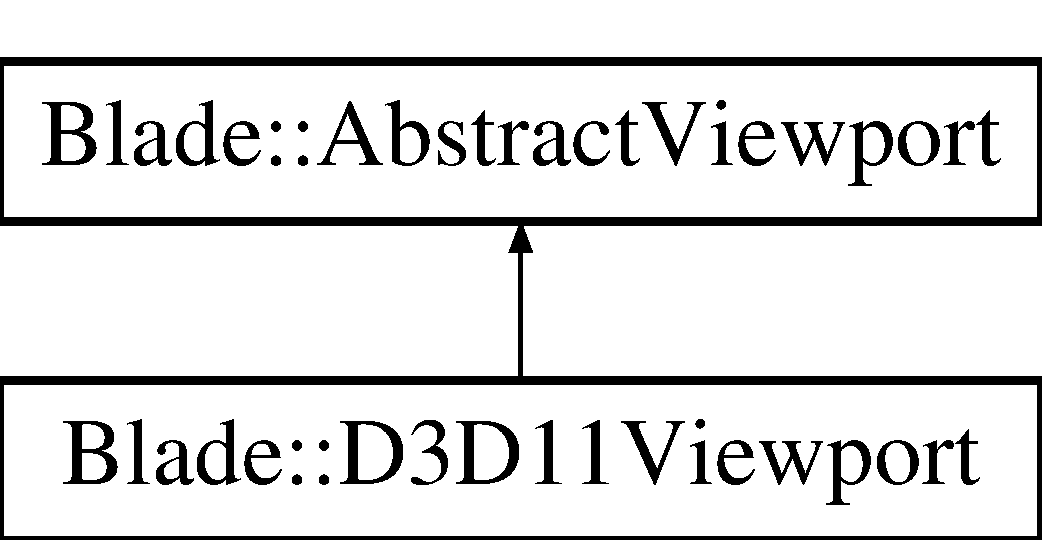
\includegraphics[height=2.000000cm]{class_blade_1_1_abstract_viewport}
\end{center}
\end{figure}
\subsection*{Public Member Functions}
\begin{DoxyCompactItemize}
\item 
\mbox{\Hypertarget{class_blade_1_1_abstract_viewport_a0962406e3c44affa7efd1f7d9175a1d4}\label{class_blade_1_1_abstract_viewport_a0962406e3c44affa7efd1f7d9175a1d4}} 
\hyperlink{class_blade_1_1_abstract_viewport_a0962406e3c44affa7efd1f7d9175a1d4}{Abstract\+Viewport} ()=default
\begin{DoxyCompactList}\small\item\em \hyperlink{class_blade_1_1_abstract_viewport}{Abstract\+Viewport}\textquotesingle{}s default constructor. \end{DoxyCompactList}\item 
\hyperlink{class_blade_1_1_abstract_viewport_aa04544ba6e933bc0e6c2e6ca878d4541}{Abstract\+Viewport} (const \hyperlink{namespace_blade_ac765e9c5c8205009994e4243d9d6f81c}{Recti} \&rect)
\begin{DoxyCompactList}\small\item\em \hyperlink{class_blade_1_1_abstract_viewport}{Abstract\+Viewport}\textquotesingle{}s constructor. \end{DoxyCompactList}\item 
\mbox{\Hypertarget{class_blade_1_1_abstract_viewport_abb8e72341ffca5fb5bd9b2891a959612}\label{class_blade_1_1_abstract_viewport_abb8e72341ffca5fb5bd9b2891a959612}} 
virtual \hyperlink{class_blade_1_1_abstract_viewport_abb8e72341ffca5fb5bd9b2891a959612}{$\sim$\+Abstract\+Viewport} ()=default
\begin{DoxyCompactList}\small\item\em \hyperlink{class_blade_1_1_abstract_viewport}{Abstract\+Viewport}\textquotesingle{}s default destructor. \end{DoxyCompactList}\item 
const \hyperlink{namespace_blade_ac765e9c5c8205009994e4243d9d6f81c}{Recti} \& \hyperlink{class_blade_1_1_abstract_viewport_abd3c922bb2552224fccea3f940160f05}{Get\+Rect} () const noexcept
\begin{DoxyCompactList}\small\item\em Provides the dimensions of the Viewport. \end{DoxyCompactList}\item 
void \hyperlink{class_blade_1_1_abstract_viewport_af229a400e575300684e8f84794ba299d}{Set\+Rect} (const \hyperlink{namespace_blade_ac765e9c5c8205009994e4243d9d6f81c}{Recti} \&rect) noexcept
\begin{DoxyCompactList}\small\item\em Sets the dimensions of the Viewport. \end{DoxyCompactList}\item 
\mbox{\Hypertarget{class_blade_1_1_abstract_viewport_a5ea486e1fbae3f6725cac10353644f24}\label{class_blade_1_1_abstract_viewport_a5ea486e1fbae3f6725cac10353644f24}} 
virtual void \hyperlink{class_blade_1_1_abstract_viewport_a5ea486e1fbae3f6725cac10353644f24}{Set} () const noexcept=0
\begin{DoxyCompactList}\small\item\em Sets the Viewport to the Rasterizer. \end{DoxyCompactList}\end{DoxyCompactItemize}


\subsection{Detailed Description}
Describes an implementation agnostic Viewport. 

\subsection{Constructor \& Destructor Documentation}
\mbox{\Hypertarget{class_blade_1_1_abstract_viewport_aa04544ba6e933bc0e6c2e6ca878d4541}\label{class_blade_1_1_abstract_viewport_aa04544ba6e933bc0e6c2e6ca878d4541}} 
\index{Blade\+::\+Abstract\+Viewport@{Blade\+::\+Abstract\+Viewport}!Abstract\+Viewport@{Abstract\+Viewport}}
\index{Abstract\+Viewport@{Abstract\+Viewport}!Blade\+::\+Abstract\+Viewport@{Blade\+::\+Abstract\+Viewport}}
\subsubsection{\texorpdfstring{Abstract\+Viewport()}{AbstractViewport()}}
{\footnotesize\ttfamily Blade\+::\+Abstract\+Viewport\+::\+Abstract\+Viewport (\begin{DoxyParamCaption}\item[{const \hyperlink{namespace_blade_ac765e9c5c8205009994e4243d9d6f81c}{Recti} \&}]{rect }\end{DoxyParamCaption})\hspace{0.3cm}{\ttfamily [inline]}, {\ttfamily [explicit]}}



\hyperlink{class_blade_1_1_abstract_viewport}{Abstract\+Viewport}\textquotesingle{}s constructor. 


\begin{DoxyParams}{Parameters}
{\em rect} & The dimensions of the Viewport. \\
\hline
\end{DoxyParams}


\subsection{Member Function Documentation}
\mbox{\Hypertarget{class_blade_1_1_abstract_viewport_abd3c922bb2552224fccea3f940160f05}\label{class_blade_1_1_abstract_viewport_abd3c922bb2552224fccea3f940160f05}} 
\index{Blade\+::\+Abstract\+Viewport@{Blade\+::\+Abstract\+Viewport}!Get\+Rect@{Get\+Rect}}
\index{Get\+Rect@{Get\+Rect}!Blade\+::\+Abstract\+Viewport@{Blade\+::\+Abstract\+Viewport}}
\subsubsection{\texorpdfstring{Get\+Rect()}{GetRect()}}
{\footnotesize\ttfamily const \hyperlink{namespace_blade_ac765e9c5c8205009994e4243d9d6f81c}{Recti} \& Blade\+::\+Abstract\+Viewport\+::\+Get\+Rect (\begin{DoxyParamCaption}{ }\end{DoxyParamCaption}) const\hspace{0.3cm}{\ttfamily [noexcept]}}



Provides the dimensions of the Viewport. 

\begin{DoxyReturn}{Returns}
The dimensions of the Viewport. 
\end{DoxyReturn}
\mbox{\Hypertarget{class_blade_1_1_abstract_viewport_af229a400e575300684e8f84794ba299d}\label{class_blade_1_1_abstract_viewport_af229a400e575300684e8f84794ba299d}} 
\index{Blade\+::\+Abstract\+Viewport@{Blade\+::\+Abstract\+Viewport}!Set\+Rect@{Set\+Rect}}
\index{Set\+Rect@{Set\+Rect}!Blade\+::\+Abstract\+Viewport@{Blade\+::\+Abstract\+Viewport}}
\subsubsection{\texorpdfstring{Set\+Rect()}{SetRect()}}
{\footnotesize\ttfamily void Blade\+::\+Abstract\+Viewport\+::\+Set\+Rect (\begin{DoxyParamCaption}\item[{const \hyperlink{namespace_blade_ac765e9c5c8205009994e4243d9d6f81c}{Recti} \&}]{rect }\end{DoxyParamCaption})\hspace{0.3cm}{\ttfamily [noexcept]}}



Sets the dimensions of the Viewport. 


\begin{DoxyParams}{Parameters}
{\em rect} & The dimensions of the Viewport. \\
\hline
\end{DoxyParams}


The documentation for this class was generated from the following files\+:\begin{DoxyCompactItemize}
\item 
include/abstract\+\_\+viewport.\+h\item 
src/abstract\+\_\+viewport.\+cpp\end{DoxyCompactItemize}

\hypertarget{class_blade_1_1_animation}{}\section{Blade\+:\+:Animation Class Reference}
\label{class_blade_1_1_animation}\index{Blade\+::\+Animation@{Blade\+::\+Animation}}
\subsection*{Public Member Functions}
\begin{DoxyCompactItemize}
\item 
\mbox{\Hypertarget{class_blade_1_1_animation_a10659aad5c72d1fd333b9b804939dfb7}\label{class_blade_1_1_animation_a10659aad5c72d1fd333b9b804939dfb7}} 
{\bfseries Animation} (const std\+::string \&name, bool loop\+State)
\item 
\mbox{\Hypertarget{class_blade_1_1_animation_aa42b5ca8436e72de50933f8b36cbbe97}\label{class_blade_1_1_animation_aa42b5ca8436e72de50933f8b36cbbe97}} 
void {\bfseries Set\+Name} (const std\+::string \&name)
\item 
\mbox{\Hypertarget{class_blade_1_1_animation_ac7218b960ec725ac46707e030f640247}\label{class_blade_1_1_animation_ac7218b960ec725ac46707e030f640247}} 
void {\bfseries Set\+Loopping} (bool loop\+State)
\item 
\mbox{\Hypertarget{class_blade_1_1_animation_a4e3f718b96a8d201b50a81c57e40cb02}\label{class_blade_1_1_animation_a4e3f718b96a8d201b50a81c57e40cb02}} 
const std\+::string \& {\bfseries Get\+Name} () const noexcept
\item 
\mbox{\Hypertarget{class_blade_1_1_animation_ab446adfe719290ffd9e09d641d147d6d}\label{class_blade_1_1_animation_ab446adfe719290ffd9e09d641d147d6d}} 
const \hyperlink{struct_blade_1_1_keyframe}{Keyframe\+Vec3f} \& {\bfseries Get\+Position\+Keyframe} (unsigned int idx) const noexcept
\item 
\mbox{\Hypertarget{class_blade_1_1_animation_a89860bfca9932bfb283a1c066e622b68}\label{class_blade_1_1_animation_a89860bfca9932bfb283a1c066e622b68}} 
const \hyperlink{struct_blade_1_1_keyframe}{Keyframe\+Quatf} \& {\bfseries Get\+Rotation\+Keyframe} (unsigned int idx) const noexcept
\item 
\mbox{\Hypertarget{class_blade_1_1_animation_a4ebb4b87cc087fb0b9c91c75d8ab5f04}\label{class_blade_1_1_animation_a4ebb4b87cc087fb0b9c91c75d8ab5f04}} 
const \hyperlink{struct_blade_1_1_keyframe}{Keyframe\+Vec3f} \& {\bfseries Get\+Scaling\+Keyframe} (unsigned int idx) const noexcept
\item 
\mbox{\Hypertarget{class_blade_1_1_animation_a1d3434e2e65348e77ef78aa4bffd0a42}\label{class_blade_1_1_animation_a1d3434e2e65348e77ef78aa4bffd0a42}} 
size\+\_\+t {\bfseries Get\+Position\+Keyframe\+Count} () const noexcept
\item 
\mbox{\Hypertarget{class_blade_1_1_animation_a99e271bc36e1bbed6488c00fccad93b6}\label{class_blade_1_1_animation_a99e271bc36e1bbed6488c00fccad93b6}} 
size\+\_\+t {\bfseries Get\+Rotation\+Keyframe\+Count} () const noexcept
\item 
\mbox{\Hypertarget{class_blade_1_1_animation_a6903d3a3728f6cc339f623e44a937bfc}\label{class_blade_1_1_animation_a6903d3a3728f6cc339f623e44a937bfc}} 
size\+\_\+t {\bfseries Get\+Scaling\+Keyframe\+Count} () const noexcept
\item 
\mbox{\Hypertarget{class_blade_1_1_animation_acbfde9c9cc2a75322cea288f6fcd9789}\label{class_blade_1_1_animation_acbfde9c9cc2a75322cea288f6fcd9789}} 
void {\bfseries Set\+Animation\+Speed} (float speed) noexcept
\item 
\mbox{\Hypertarget{class_blade_1_1_animation_a55b59bafd53b9e38ad71b38cbc3e2ff0}\label{class_blade_1_1_animation_a55b59bafd53b9e38ad71b38cbc3e2ff0}} 
float {\bfseries Get\+Animation\+Speed} () const noexcept
\item 
\mbox{\Hypertarget{class_blade_1_1_animation_a0d32b8a4ca6f549cce9842a7d8d5ff84}\label{class_blade_1_1_animation_a0d32b8a4ca6f549cce9842a7d8d5ff84}} 
bool {\bfseries Has\+Position\+Keyframes} () const noexcept
\item 
\mbox{\Hypertarget{class_blade_1_1_animation_a6325e0249448d0cd7b1b780872906580}\label{class_blade_1_1_animation_a6325e0249448d0cd7b1b780872906580}} 
bool {\bfseries Has\+Rotation\+Keyframes} () const noexcept
\item 
\mbox{\Hypertarget{class_blade_1_1_animation_a7886bf10e255deaafbb358e059195688}\label{class_blade_1_1_animation_a7886bf10e255deaafbb358e059195688}} 
bool {\bfseries Has\+Scaling\+Keyframes} () const noexcept
\item 
\mbox{\Hypertarget{class_blade_1_1_animation_a255de6c54b74c466b0f140292cf0e7d4}\label{class_blade_1_1_animation_a255de6c54b74c466b0f140292cf0e7d4}} 
bool {\bfseries Does\+Loop} () const noexcept
\item 
\mbox{\Hypertarget{class_blade_1_1_animation_a143e5c92e121518649af8a66758df4ff}\label{class_blade_1_1_animation_a143e5c92e121518649af8a66758df4ff}} 
void {\bfseries Add\+Position\+Keyframe} (const \hyperlink{struct_blade_1_1_keyframe}{Keyframe\+Vec3f} \&pos) noexcept
\item 
\mbox{\Hypertarget{class_blade_1_1_animation_a443dc6dcb392227104fe1727ed7b411c}\label{class_blade_1_1_animation_a443dc6dcb392227104fe1727ed7b411c}} 
void {\bfseries Add\+Rotation\+Keyframe} (const \hyperlink{struct_blade_1_1_keyframe}{Keyframe\+Quatf} \&rot) noexcept
\item 
\mbox{\Hypertarget{class_blade_1_1_animation_ad8f71fb524d1e54dec1404dee61c0cd2}\label{class_blade_1_1_animation_ad8f71fb524d1e54dec1404dee61c0cd2}} 
void {\bfseries Add\+Scaling\+Keyframe} (const \hyperlink{struct_blade_1_1_keyframe}{Keyframe\+Vec3f} \&scaling) noexcept
\item 
\mbox{\Hypertarget{class_blade_1_1_animation_a8474b5ddb86f562ee9b8442ea99579a9}\label{class_blade_1_1_animation_a8474b5ddb86f562ee9b8442ea99579a9}} 
void {\bfseries Replace\+Position\+Keyframe} (const \hyperlink{struct_blade_1_1_keyframe}{Keyframe\+Vec3f} \&pos, unsigned int idx) noexcept
\item 
\mbox{\Hypertarget{class_blade_1_1_animation_abcaaaf273da130260b713c2366d009a8}\label{class_blade_1_1_animation_abcaaaf273da130260b713c2366d009a8}} 
void {\bfseries Replace\+Rotation\+Keyframe} (const \hyperlink{struct_blade_1_1_keyframe}{Keyframe\+Quatf} \&rot, unsigned int idx) noexcept
\item 
\mbox{\Hypertarget{class_blade_1_1_animation_acaa08703ede629aac7259ed696bb92f9}\label{class_blade_1_1_animation_acaa08703ede629aac7259ed696bb92f9}} 
void {\bfseries Replace\+Scaling\+Keyframe} (const \hyperlink{struct_blade_1_1_keyframe}{Keyframe\+Vec3f} \&scaling, unsigned int idx) noexcept
\item 
\mbox{\Hypertarget{class_blade_1_1_animation_a4e627c0196f9a0990cde2c454f853b11}\label{class_blade_1_1_animation_a4e627c0196f9a0990cde2c454f853b11}} 
void {\bfseries Clear\+Keyframes} () noexcept
\item 
\mbox{\Hypertarget{class_blade_1_1_animation_aa723894052e5f46e73c762df2ae55532}\label{class_blade_1_1_animation_aa723894052e5f46e73c762df2ae55532}} 
void {\bfseries Sort\+Position\+Keyframes} () noexcept
\item 
\mbox{\Hypertarget{class_blade_1_1_animation_a3b7022dfd85c88327f5e32bd6e393bb1}\label{class_blade_1_1_animation_a3b7022dfd85c88327f5e32bd6e393bb1}} 
void {\bfseries Sort\+Rotation\+Keyframes} () noexcept
\item 
\mbox{\Hypertarget{class_blade_1_1_animation_a5f37f7a7be8395100d0797cb7019907a}\label{class_blade_1_1_animation_a5f37f7a7be8395100d0797cb7019907a}} 
void {\bfseries Sort\+Scaling\+Keyframes} () noexcept
\end{DoxyCompactItemize}


The documentation for this class was generated from the following files\+:\begin{DoxyCompactItemize}
\item 
include/animation.\+h\item 
src/animation.\+cpp\end{DoxyCompactItemize}

\hypertarget{class_blade_1_1_application}{}\section{Blade\+:\+:Application Class Reference}
\label{class_blade_1_1_application}\index{Blade\+::\+Application@{Blade\+::\+Application}}


\hyperlink{class_blade_1_1_application}{Application} class of the engine.  




{\ttfamily \#include $<$application.\+h$>$}

\subsection*{Public Member Functions}
\begin{DoxyCompactItemize}
\item 
\mbox{\Hypertarget{class_blade_1_1_application_a73ea9e8a20297c3dd47a565302e46b10}\label{class_blade_1_1_application_a73ea9e8a20297c3dd47a565302e46b10}} 
{\bfseries Application} (const \hyperlink{class_blade_1_1_application}{Application} \&application)=delete
\item 
\mbox{\Hypertarget{class_blade_1_1_application_ad7528afe280f12aa19f0dcbefd5083aa}\label{class_blade_1_1_application_ad7528afe280f12aa19f0dcbefd5083aa}} 
\hyperlink{class_blade_1_1_application}{Application} \& {\bfseries operator=} (const \hyperlink{class_blade_1_1_application}{Application} \&application)=delete
\item 
void \hyperlink{class_blade_1_1_application_a74d0bed9493b107ac522db1a40ebe19d}{Set\+Termination} (bool state) noexcept
\begin{DoxyCompactList}\small\item\em Set the termination flag. \end{DoxyCompactList}\item 
bool \hyperlink{class_blade_1_1_application_a68aba5838320ebb7b2683954ffee050b}{Should\+Terminate} () const noexcept
\begin{DoxyCompactList}\small\item\em Return the should terminate flag. \end{DoxyCompactList}\item 
double \hyperlink{class_blade_1_1_application_a8e144f5f05fc638339fc19afe142bbab}{Get\+Delta} () const noexcept
\begin{DoxyCompactList}\small\item\em Get the delta time of the application. \end{DoxyCompactList}\item 
long \hyperlink{class_blade_1_1_application_a0fd401f7a7ea78a8d222ccc920cb1968}{Get\+Msec} () const noexcept
\begin{DoxyCompactList}\small\item\em Get the time elapse since the startup in milliseconds. \end{DoxyCompactList}\item 
double \hyperlink{class_blade_1_1_application_a025118e872031944df57560e820cfde2}{Get\+Sec} () const noexcept
\begin{DoxyCompactList}\small\item\em Get the time elapsed since the startup in seconds. \end{DoxyCompactList}\item 
\mbox{\Hypertarget{class_blade_1_1_application_a3c8f0f5698682bd2b205ae1616020073}\label{class_blade_1_1_application_a3c8f0f5698682bd2b205ae1616020073}} 
void \hyperlink{class_blade_1_1_application_a3c8f0f5698682bd2b205ae1616020073}{Pause} () noexcept
\begin{DoxyCompactList}\small\item\em Pause the application. \end{DoxyCompactList}\item 
\mbox{\Hypertarget{class_blade_1_1_application_ab8626a9bc16bffa5d94d2e5851e378a2}\label{class_blade_1_1_application_ab8626a9bc16bffa5d94d2e5851e378a2}} 
void \hyperlink{class_blade_1_1_application_ab8626a9bc16bffa5d94d2e5851e378a2}{Un\+Pause} () noexcept
\begin{DoxyCompactList}\small\item\em Un pause the application. \end{DoxyCompactList}\item 
bool \hyperlink{class_blade_1_1_application_a80cb2abe5d175dde76be4f461bd82183}{Is\+Paused} () const noexcept
\begin{DoxyCompactList}\small\item\em Check if the application is paused. \end{DoxyCompactList}\item 
void \hyperlink{class_blade_1_1_application_a328d42f7cb14a418ad3b9c54aa055132}{Set\+Load\+Entity\+Callback} (const Load\+Entity\+Callback \&callback) noexcept
\begin{DoxyCompactList}\small\item\em Set the load entity call back. \end{DoxyCompactList}\item 
const Load\+Entity\+Callback \& \hyperlink{class_blade_1_1_application_ac5964be32df8e0787b832896c0811ae6}{Get\+Load\+Entity\+Callback} () const noexcept
\begin{DoxyCompactList}\small\item\em Get the load entity call back of the engine. \end{DoxyCompactList}\item 
\mbox{\Hypertarget{class_blade_1_1_application_a5abbd8e3d830a6543f4abbc2d100c562}\label{class_blade_1_1_application_a5abbd8e3d830a6543f4abbc2d100c562}} 
virtual bool \hyperlink{class_blade_1_1_application_a5abbd8e3d830a6543f4abbc2d100c562}{Initialize} (int $\ast$argc, char $\ast$argv\mbox{[}$\,$\mbox{]})
\begin{DoxyCompactList}\small\item\em Initialize the application. \end{DoxyCompactList}\item 
\mbox{\Hypertarget{class_blade_1_1_application_a18b70b1a66b3c639e723464a0f31cc5f}\label{class_blade_1_1_application_a18b70b1a66b3c639e723464a0f31cc5f}} 
virtual void \hyperlink{class_blade_1_1_application_a18b70b1a66b3c639e723464a0f31cc5f}{Update} () noexcept=0
\begin{DoxyCompactList}\small\item\em Update the application. \end{DoxyCompactList}\item 
\mbox{\Hypertarget{class_blade_1_1_application_a660b728e2e7855548d02316c328da2f7}\label{class_blade_1_1_application_a660b728e2e7855548d02316c328da2f7}} 
virtual void \hyperlink{class_blade_1_1_application_a660b728e2e7855548d02316c328da2f7}{Draw} () const noexcept=0
\begin{DoxyCompactList}\small\item\em Draw the application on screen. \end{DoxyCompactList}\item 
\mbox{\Hypertarget{class_blade_1_1_application_a969f20210bd185cc6912b7794a0eea5b}\label{class_blade_1_1_application_a969f20210bd185cc6912b7794a0eea5b}} 
virtual int \hyperlink{class_blade_1_1_application_a969f20210bd185cc6912b7794a0eea5b}{Run} () noexcept=0
\begin{DoxyCompactList}\small\item\em Run the application. \end{DoxyCompactList}\end{DoxyCompactItemize}


\subsection{Detailed Description}
\hyperlink{class_blade_1_1_application}{Application} class of the engine. 

\subsection{Member Function Documentation}
\mbox{\Hypertarget{class_blade_1_1_application_a8e144f5f05fc638339fc19afe142bbab}\label{class_blade_1_1_application_a8e144f5f05fc638339fc19afe142bbab}} 
\index{Blade\+::\+Application@{Blade\+::\+Application}!Get\+Delta@{Get\+Delta}}
\index{Get\+Delta@{Get\+Delta}!Blade\+::\+Application@{Blade\+::\+Application}}
\subsubsection{\texorpdfstring{Get\+Delta()}{GetDelta()}}
{\footnotesize\ttfamily double Blade\+::\+Application\+::\+Get\+Delta (\begin{DoxyParamCaption}{ }\end{DoxyParamCaption}) const\hspace{0.3cm}{\ttfamily [noexcept]}}



Get the delta time of the application. 

\begin{DoxyReturn}{Returns}
The delta time. 
\end{DoxyReturn}
\mbox{\Hypertarget{class_blade_1_1_application_ac5964be32df8e0787b832896c0811ae6}\label{class_blade_1_1_application_ac5964be32df8e0787b832896c0811ae6}} 
\index{Blade\+::\+Application@{Blade\+::\+Application}!Get\+Load\+Entity\+Callback@{Get\+Load\+Entity\+Callback}}
\index{Get\+Load\+Entity\+Callback@{Get\+Load\+Entity\+Callback}!Blade\+::\+Application@{Blade\+::\+Application}}
\subsubsection{\texorpdfstring{Get\+Load\+Entity\+Callback()}{GetLoadEntityCallback()}}
{\footnotesize\ttfamily const Load\+Entity\+Callback \& Blade\+::\+Application\+::\+Get\+Load\+Entity\+Callback (\begin{DoxyParamCaption}{ }\end{DoxyParamCaption}) const\hspace{0.3cm}{\ttfamily [noexcept]}}



Get the load entity call back of the engine. 

\begin{DoxyReturn}{Returns}
The callback used to load entities. 
\end{DoxyReturn}
\mbox{\Hypertarget{class_blade_1_1_application_a0fd401f7a7ea78a8d222ccc920cb1968}\label{class_blade_1_1_application_a0fd401f7a7ea78a8d222ccc920cb1968}} 
\index{Blade\+::\+Application@{Blade\+::\+Application}!Get\+Msec@{Get\+Msec}}
\index{Get\+Msec@{Get\+Msec}!Blade\+::\+Application@{Blade\+::\+Application}}
\subsubsection{\texorpdfstring{Get\+Msec()}{GetMsec()}}
{\footnotesize\ttfamily long Blade\+::\+Application\+::\+Get\+Msec (\begin{DoxyParamCaption}{ }\end{DoxyParamCaption}) const\hspace{0.3cm}{\ttfamily [noexcept]}}



Get the time elapse since the startup in milliseconds. 

\begin{DoxyReturn}{Returns}
time elapsed in milliseconds 
\end{DoxyReturn}
\mbox{\Hypertarget{class_blade_1_1_application_a025118e872031944df57560e820cfde2}\label{class_blade_1_1_application_a025118e872031944df57560e820cfde2}} 
\index{Blade\+::\+Application@{Blade\+::\+Application}!Get\+Sec@{Get\+Sec}}
\index{Get\+Sec@{Get\+Sec}!Blade\+::\+Application@{Blade\+::\+Application}}
\subsubsection{\texorpdfstring{Get\+Sec()}{GetSec()}}
{\footnotesize\ttfamily double Blade\+::\+Application\+::\+Get\+Sec (\begin{DoxyParamCaption}{ }\end{DoxyParamCaption}) const\hspace{0.3cm}{\ttfamily [noexcept]}}



Get the time elapsed since the startup in seconds. 

\begin{DoxyReturn}{Returns}
time elapsed in seconds. 
\end{DoxyReturn}
\mbox{\Hypertarget{class_blade_1_1_application_a80cb2abe5d175dde76be4f461bd82183}\label{class_blade_1_1_application_a80cb2abe5d175dde76be4f461bd82183}} 
\index{Blade\+::\+Application@{Blade\+::\+Application}!Is\+Paused@{Is\+Paused}}
\index{Is\+Paused@{Is\+Paused}!Blade\+::\+Application@{Blade\+::\+Application}}
\subsubsection{\texorpdfstring{Is\+Paused()}{IsPaused()}}
{\footnotesize\ttfamily bool Blade\+::\+Application\+::\+Is\+Paused (\begin{DoxyParamCaption}{ }\end{DoxyParamCaption}) const\hspace{0.3cm}{\ttfamily [noexcept]}}



Check if the application is paused. 

\begin{DoxyReturn}{Returns}
T\+R\+UE if the application is paused, F\+A\+L\+SE otherwise 
\end{DoxyReturn}
\mbox{\Hypertarget{class_blade_1_1_application_a328d42f7cb14a418ad3b9c54aa055132}\label{class_blade_1_1_application_a328d42f7cb14a418ad3b9c54aa055132}} 
\index{Blade\+::\+Application@{Blade\+::\+Application}!Set\+Load\+Entity\+Callback@{Set\+Load\+Entity\+Callback}}
\index{Set\+Load\+Entity\+Callback@{Set\+Load\+Entity\+Callback}!Blade\+::\+Application@{Blade\+::\+Application}}
\subsubsection{\texorpdfstring{Set\+Load\+Entity\+Callback()}{SetLoadEntityCallback()}}
{\footnotesize\ttfamily void Blade\+::\+Application\+::\+Set\+Load\+Entity\+Callback (\begin{DoxyParamCaption}\item[{const Load\+Entity\+Callback \&}]{callback }\end{DoxyParamCaption})\hspace{0.3cm}{\ttfamily [noexcept]}}



Set the load entity call back. 


\begin{DoxyParams}{Parameters}
{\em callback} & The callback used to load entities from file. \\
\hline
\end{DoxyParams}
\mbox{\Hypertarget{class_blade_1_1_application_a74d0bed9493b107ac522db1a40ebe19d}\label{class_blade_1_1_application_a74d0bed9493b107ac522db1a40ebe19d}} 
\index{Blade\+::\+Application@{Blade\+::\+Application}!Set\+Termination@{Set\+Termination}}
\index{Set\+Termination@{Set\+Termination}!Blade\+::\+Application@{Blade\+::\+Application}}
\subsubsection{\texorpdfstring{Set\+Termination()}{SetTermination()}}
{\footnotesize\ttfamily void Blade\+::\+Application\+::\+Set\+Termination (\begin{DoxyParamCaption}\item[{bool}]{state }\end{DoxyParamCaption})\hspace{0.3cm}{\ttfamily [noexcept]}}



Set the termination flag. 


\begin{DoxyParams}{Parameters}
{\em state} & The state of the application to set. \\
\hline
\end{DoxyParams}
\mbox{\Hypertarget{class_blade_1_1_application_a68aba5838320ebb7b2683954ffee050b}\label{class_blade_1_1_application_a68aba5838320ebb7b2683954ffee050b}} 
\index{Blade\+::\+Application@{Blade\+::\+Application}!Should\+Terminate@{Should\+Terminate}}
\index{Should\+Terminate@{Should\+Terminate}!Blade\+::\+Application@{Blade\+::\+Application}}
\subsubsection{\texorpdfstring{Should\+Terminate()}{ShouldTerminate()}}
{\footnotesize\ttfamily bool Blade\+::\+Application\+::\+Should\+Terminate (\begin{DoxyParamCaption}{ }\end{DoxyParamCaption}) const\hspace{0.3cm}{\ttfamily [noexcept]}}



Return the should terminate flag. 

\begin{DoxyReturn}{Returns}
T\+R\+UE if the application should terminate, false otherwise 
\end{DoxyReturn}


The documentation for this class was generated from the following files\+:\begin{DoxyCompactItemize}
\item 
include/application.\+h\item 
src/application.\+cpp\end{DoxyCompactItemize}

\hypertarget{class_blade_1_1_audio_manager}{}\section{Blade\+:\+:Audio\+Manager Class Reference}
\label{class_blade_1_1_audio_manager}\index{Blade\+::\+Audio\+Manager@{Blade\+::\+Audio\+Manager}}
\subsection*{Public Member Functions}
\begin{DoxyCompactItemize}
\item 
\mbox{\Hypertarget{class_blade_1_1_audio_manager_a1106ccc2bbab55f49024eb5502d10683}\label{class_blade_1_1_audio_manager_a1106ccc2bbab55f49024eb5502d10683}} 
void {\bfseries Set\+Sources\+Volume} (float volume)
\item 
\mbox{\Hypertarget{class_blade_1_1_audio_manager_a3d3199ddf491cc32f41e8d3252485176}\label{class_blade_1_1_audio_manager_a3d3199ddf491cc32f41e8d3252485176}} 
void {\bfseries Set\+Streams\+Volume} (float volume)
\item 
\mbox{\Hypertarget{class_blade_1_1_audio_manager_acb30e9b4b523989514703d943e659f92}\label{class_blade_1_1_audio_manager_acb30e9b4b523989514703d943e659f92}} 
void {\bfseries Set\+Master\+Volume} (float volume)
\item 
\mbox{\Hypertarget{class_blade_1_1_audio_manager_abbea9e3d1d332c983b86d8a2eea926b4}\label{class_blade_1_1_audio_manager_abbea9e3d1d332c983b86d8a2eea926b4}} 
\hyperlink{class_blade_1_1_ogg_vorbis_stream}{Ogg\+Vorbis\+Stream} $\ast$ {\bfseries Get\+Audio\+Stream} (int idx)
\item 
\mbox{\Hypertarget{class_blade_1_1_audio_manager_a3956140c9454c2d41adeaf5f0e15d455}\label{class_blade_1_1_audio_manager_a3956140c9454c2d41adeaf5f0e15d455}} 
\hyperlink{class_blade_1_1_audio_source}{Audio\+Source} $\ast$ {\bfseries Get\+Audio\+Source} (int idx)
\item 
\mbox{\Hypertarget{class_blade_1_1_audio_manager_af9e3f8dbd2f825a6166b35b275632d50}\label{class_blade_1_1_audio_manager_af9e3f8dbd2f825a6166b35b275632d50}} 
\hyperlink{class_blade_1_1_audio_source}{Audio\+Source} $\ast$ {\bfseries Get\+Audio\+Source} (\hyperlink{class_blade_1_1_audio_sample}{Audio\+Sample} $\ast$sample)
\item 
\mbox{\Hypertarget{class_blade_1_1_audio_manager_ac62793fe1189d24009b5e5d9e33d33b0}\label{class_blade_1_1_audio_manager_ac62793fe1189d24009b5e5d9e33d33b0}} 
void {\bfseries Play\+Stream} (const std\+::wstring \&fname, float volume, Audio\+Playmode mode, int $\ast$stream\+\_\+idx=nullptr)
\item 
\mbox{\Hypertarget{class_blade_1_1_audio_manager_a38aa61aff48af21489ef9096f4888d30}\label{class_blade_1_1_audio_manager_a38aa61aff48af21489ef9096f4888d30}} 
void {\bfseries Play\+Sample} (\hyperlink{class_blade_1_1_audio_sample}{Audio\+Sample} $\ast$sample, float volume, Audio\+Playmode mode, const Vec3f \&position=Vec3f\{ 0, 0, 0 \}, int $\ast$src\+\_\+idx=nullptr)
\item 
\mbox{\Hypertarget{class_blade_1_1_audio_manager_a38dd034452d867957586cc47686bcb9a}\label{class_blade_1_1_audio_manager_a38dd034452d867957586cc47686bcb9a}} 
void {\bfseries Play\+Stream\+Playlist} (\hyperlink{struct_blade_1_1_stream_playlist}{Stream\+Playlist} $\ast$playlist, float volume)
\item 
\mbox{\Hypertarget{class_blade_1_1_audio_manager_a166ea37858554e2cc6b97b4aaea9797b}\label{class_blade_1_1_audio_manager_a166ea37858554e2cc6b97b4aaea9797b}} 
void {\bfseries Play\+Sample\+Playlist} (\hyperlink{struct_blade_1_1_sample_playlist}{Sample\+Playlist} $\ast$playlist, float volume)
\item 
\mbox{\Hypertarget{class_blade_1_1_audio_manager_a79acd2f6a2933ce8ed2eea139b388b93}\label{class_blade_1_1_audio_manager_a79acd2f6a2933ce8ed2eea139b388b93}} 
void {\bfseries Stop\+Stream} (int stream\+\_\+idx)
\item 
\mbox{\Hypertarget{class_blade_1_1_audio_manager_abe8fbb12bfb5dff14e4cd000fd55b266}\label{class_blade_1_1_audio_manager_abe8fbb12bfb5dff14e4cd000fd55b266}} 
void {\bfseries Stop\+Source} (int source\+\_\+idx)
\item 
\mbox{\Hypertarget{class_blade_1_1_audio_manager_aef2463b40b6c97a3d4f2b9a72fc13f48}\label{class_blade_1_1_audio_manager_aef2463b40b6c97a3d4f2b9a72fc13f48}} 
void {\bfseries Stop\+Streams} ()
\item 
\mbox{\Hypertarget{class_blade_1_1_audio_manager_a2112e72e111040c5f8c32b6d615d63bc}\label{class_blade_1_1_audio_manager_a2112e72e111040c5f8c32b6d615d63bc}} 
void {\bfseries Stop\+Sources} ()
\item 
\mbox{\Hypertarget{class_blade_1_1_audio_manager_ae554f09a7f929114d7ce150b7b84af79}\label{class_blade_1_1_audio_manager_ae554f09a7f929114d7ce150b7b84af79}} 
void {\bfseries Pause\+Streams} ()
\item 
\mbox{\Hypertarget{class_blade_1_1_audio_manager_aa09b17fa1814554e1f85e23c17049a4a}\label{class_blade_1_1_audio_manager_aa09b17fa1814554e1f85e23c17049a4a}} 
void {\bfseries Pause\+Sources} ()
\item 
\mbox{\Hypertarget{class_blade_1_1_audio_manager_ac3ed228e08f3cafa52ab206fc42ba745}\label{class_blade_1_1_audio_manager_ac3ed228e08f3cafa52ab206fc42ba745}} 
void {\bfseries Resume\+Streams} ()
\item 
\mbox{\Hypertarget{class_blade_1_1_audio_manager_ab354d7e20969467d0d42bf1050d850be}\label{class_blade_1_1_audio_manager_ab354d7e20969467d0d42bf1050d850be}} 
void {\bfseries Resume\+Sources} ()
\item 
\mbox{\Hypertarget{class_blade_1_1_audio_manager_ade6ee47743387983ad56e1c77fc6c1a3}\label{class_blade_1_1_audio_manager_ade6ee47743387983ad56e1c77fc6c1a3}} 
void {\bfseries Regulate\+Volumes} ()
\end{DoxyCompactItemize}
\subsection*{Static Public Member Functions}
\begin{DoxyCompactItemize}
\item 
\mbox{\Hypertarget{class_blade_1_1_audio_manager_aba33e3e3cabd2a49170f1937f9b70a37}\label{class_blade_1_1_audio_manager_aba33e3e3cabd2a49170f1937f9b70a37}} 
static void {\bfseries Set\+Listener\+Position} (const Vec3f \&pos=Vec3f\{ 0, 0, 0 \})
\item 
\mbox{\Hypertarget{class_blade_1_1_audio_manager_a549b33f8f8d41a1c6d92cfe0c6c5a284}\label{class_blade_1_1_audio_manager_a549b33f8f8d41a1c6d92cfe0c6c5a284}} 
static void {\bfseries Set\+Listener\+Orientation} (const Vec3f \&dir, const Vec3f \&up=Vec3f\{ 0, 1, 0 \})
\end{DoxyCompactItemize}


The documentation for this class was generated from the following files\+:\begin{DoxyCompactItemize}
\item 
include/audio\+\_\+manager.\+h\item 
src/audio\+\_\+manager.\+cpp\end{DoxyCompactItemize}

\hypertarget{class_blade_1_1_audio_sample}{}\section{Blade\+:\+:Audio\+Sample Class Reference}
\label{class_blade_1_1_audio_sample}\index{Blade\+::\+Audio\+Sample@{Blade\+::\+Audio\+Sample}}
Inheritance diagram for Blade\+:\+:Audio\+Sample\+:\begin{figure}[H]
\begin{center}
\leavevmode
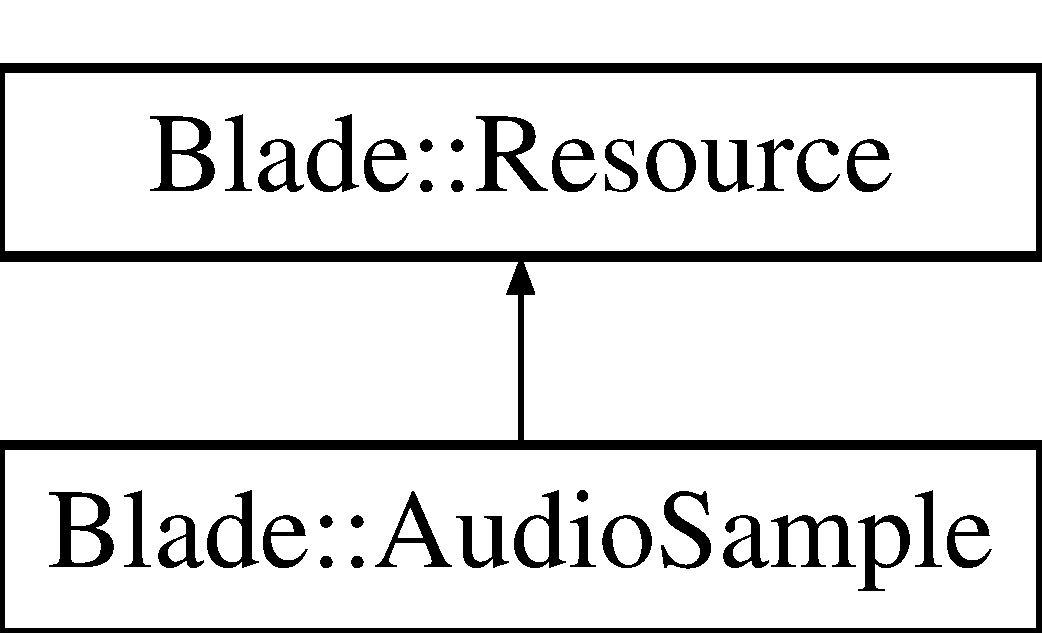
\includegraphics[height=2.000000cm]{class_blade_1_1_audio_sample}
\end{center}
\end{figure}
\subsection*{Public Member Functions}
\begin{DoxyCompactItemize}
\item 
bool \hyperlink{class_blade_1_1_audio_sample_a27bc4a11067251a2c820f1e3096bb812}{Load} (const std\+::wstring \&file\+Name) noexcept override
\begin{DoxyCompactList}\small\item\em Load a resource form a file. \end{DoxyCompactList}\item 
\mbox{\Hypertarget{class_blade_1_1_audio_sample_aa3d39cda7e85c59924022e17272dbb26}\label{class_blade_1_1_audio_sample_aa3d39cda7e85c59924022e17272dbb26}} 
unsigned int {\bfseries Get\+Buffer} () const noexcept
\end{DoxyCompactItemize}


\subsection{Member Function Documentation}
\mbox{\Hypertarget{class_blade_1_1_audio_sample_a27bc4a11067251a2c820f1e3096bb812}\label{class_blade_1_1_audio_sample_a27bc4a11067251a2c820f1e3096bb812}} 
\index{Blade\+::\+Audio\+Sample@{Blade\+::\+Audio\+Sample}!Load@{Load}}
\index{Load@{Load}!Blade\+::\+Audio\+Sample@{Blade\+::\+Audio\+Sample}}
\subsubsection{\texorpdfstring{Load()}{Load()}}
{\footnotesize\ttfamily bool Blade\+::\+Audio\+Sample\+::\+Load (\begin{DoxyParamCaption}\item[{const std\+::wstring \&}]{file\+\_\+name }\end{DoxyParamCaption})\hspace{0.3cm}{\ttfamily [override]}, {\ttfamily [virtual]}, {\ttfamily [noexcept]}}



Load a resource form a file. 


\begin{DoxyParams}{Parameters}
{\em file\+\_\+name} & The path of the file where the resource is stored. \\
\hline
\end{DoxyParams}
\begin{DoxyReturn}{Returns}
T\+R\+UE if the loading has been successful, false otherwise. 
\end{DoxyReturn}


Implements \hyperlink{class_blade_1_1_resource_ad89ab00a3b81df1338a8310ec92c5cff}{Blade\+::\+Resource}.



The documentation for this class was generated from the following files\+:\begin{DoxyCompactItemize}
\item 
include/sample.\+h\item 
src/sample.\+cpp\end{DoxyCompactItemize}

\hypertarget{class_blade_1_1_audio_source}{}\section{Blade\+:\+:Audio\+Source Class Reference}
\label{class_blade_1_1_audio_source}\index{Blade\+::\+Audio\+Source@{Blade\+::\+Audio\+Source}}
\subsection*{Public Member Functions}
\begin{DoxyCompactItemize}
\item 
\mbox{\Hypertarget{class_blade_1_1_audio_source_a9a4faa7c65dc5559d37f805791120677}\label{class_blade_1_1_audio_source_a9a4faa7c65dc5559d37f805791120677}} 
void {\bfseries Set\+Sample} (const \hyperlink{class_blade_1_1_audio_sample}{Audio\+Sample} $\ast$sample) noexcept
\item 
\mbox{\Hypertarget{class_blade_1_1_audio_source_acc604939d626bb629ce91868066a8873}\label{class_blade_1_1_audio_source_acc604939d626bb629ce91868066a8873}} 
const \hyperlink{class_blade_1_1_audio_sample}{Audio\+Sample} $\ast$ {\bfseries Get\+Sample} () const noexcept
\item 
\mbox{\Hypertarget{class_blade_1_1_audio_source_aac7f6a734c4b4dead31da9e91754aec3}\label{class_blade_1_1_audio_source_aac7f6a734c4b4dead31da9e91754aec3}} 
void {\bfseries Set\+Position} (const Vec3f \&pos, bool viewspace=false) const noexcept
\item 
\mbox{\Hypertarget{class_blade_1_1_audio_source_a64e1100ee8e1513fe85e1df82ba3fa1f}\label{class_blade_1_1_audio_source_a64e1100ee8e1513fe85e1df82ba3fa1f}} 
Vec3f {\bfseries Get\+Position} () const noexcept
\item 
\mbox{\Hypertarget{class_blade_1_1_audio_source_acc2be0ec2cd9da234850f2a77eebdcc8}\label{class_blade_1_1_audio_source_acc2be0ec2cd9da234850f2a77eebdcc8}} 
void {\bfseries Set\+Volume} (float vol) noexcept
\item 
\mbox{\Hypertarget{class_blade_1_1_audio_source_a82d9fc4bfdd71e6dd912118dd4193f31}\label{class_blade_1_1_audio_source_a82d9fc4bfdd71e6dd912118dd4193f31}} 
float {\bfseries Get\+Volume} () const noexcept
\item 
\mbox{\Hypertarget{class_blade_1_1_audio_source_a6addfca8be12a2f774403f48eb47a0f3}\label{class_blade_1_1_audio_source_a6addfca8be12a2f774403f48eb47a0f3}} 
void {\bfseries Set\+Playback\+Volume} (float vol) const noexcept
\item 
\mbox{\Hypertarget{class_blade_1_1_audio_source_a574b502ba98c588bbdebeb8c10f6f118}\label{class_blade_1_1_audio_source_a574b502ba98c588bbdebeb8c10f6f118}} 
float {\bfseries Get\+Playback\+Volume} () const noexcept
\item 
\mbox{\Hypertarget{class_blade_1_1_audio_source_a48912e741c6f38e5bc1048373d79ce09}\label{class_blade_1_1_audio_source_a48912e741c6f38e5bc1048373d79ce09}} 
void {\bfseries Set\+Looping} (bool state) const noexcept
\item 
\mbox{\Hypertarget{class_blade_1_1_audio_source_a7037c88c499d146307814fdd6487b697}\label{class_blade_1_1_audio_source_a7037c88c499d146307814fdd6487b697}} 
void {\bfseries Set\+Reference\+Dist} (float rdist) const noexcept
\item 
\mbox{\Hypertarget{class_blade_1_1_audio_source_a3af631375e1e2cf31edf79eff27502e7}\label{class_blade_1_1_audio_source_a3af631375e1e2cf31edf79eff27502e7}} 
float {\bfseries Get\+Reference\+Dist} () const noexcept
\item 
\mbox{\Hypertarget{class_blade_1_1_audio_source_a94fbc18291fb18dfc98751856411e982}\label{class_blade_1_1_audio_source_a94fbc18291fb18dfc98751856411e982}} 
void {\bfseries Set\+Max\+Dist} (float dist) const noexcept
\item 
\mbox{\Hypertarget{class_blade_1_1_audio_source_a688512119875d5be87789f9fab2a14de}\label{class_blade_1_1_audio_source_a688512119875d5be87789f9fab2a14de}} 
float {\bfseries Get\+Max\+Dist} () const noexcept
\item 
\mbox{\Hypertarget{class_blade_1_1_audio_source_aba0f76eaa86fd06ee391bf1955d63a2b}\label{class_blade_1_1_audio_source_aba0f76eaa86fd06ee391bf1955d63a2b}} 
bool {\bfseries Is\+Playing} () const noexcept
\item 
\mbox{\Hypertarget{class_blade_1_1_audio_source_a0ec6e8f896311a34b58656a199840484}\label{class_blade_1_1_audio_source_a0ec6e8f896311a34b58656a199840484}} 
bool {\bfseries Is\+Paused} () const noexcept
\item 
\mbox{\Hypertarget{class_blade_1_1_audio_source_a8f3245c3e67a68a54b4044c795657b8d}\label{class_blade_1_1_audio_source_a8f3245c3e67a68a54b4044c795657b8d}} 
void {\bfseries Play} () const noexcept
\item 
\mbox{\Hypertarget{class_blade_1_1_audio_source_a87734411556d305a366f9e3e8c00dd54}\label{class_blade_1_1_audio_source_a87734411556d305a366f9e3e8c00dd54}} 
void {\bfseries Stop} () const noexcept
\item 
\mbox{\Hypertarget{class_blade_1_1_audio_source_a4a27075da58751f49efbee1f3d3a5c86}\label{class_blade_1_1_audio_source_a4a27075da58751f49efbee1f3d3a5c86}} 
void {\bfseries Pause} () const noexcept
\end{DoxyCompactItemize}


The documentation for this class was generated from the following files\+:\begin{DoxyCompactItemize}
\item 
include/source.\+h\item 
src/source.\+cpp\end{DoxyCompactItemize}

\hypertarget{class_blade_1_1_audio_stream}{}\section{Blade\+:\+:Audio\+Stream Class Reference}
\label{class_blade_1_1_audio_stream}\index{Blade\+::\+Audio\+Stream@{Blade\+::\+Audio\+Stream}}
Inheritance diagram for Blade\+:\+:Audio\+Stream\+:\begin{figure}[H]
\begin{center}
\leavevmode
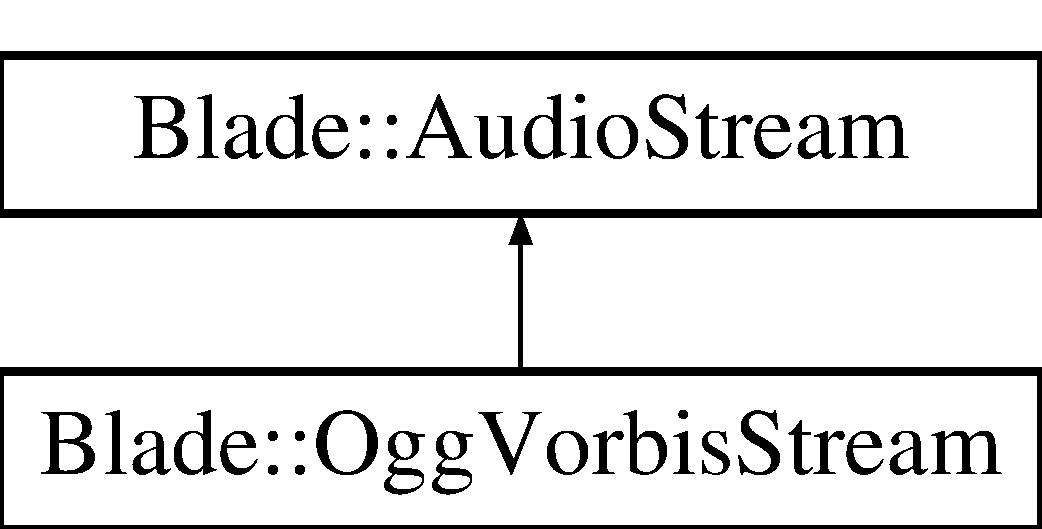
\includegraphics[height=2.000000cm]{class_blade_1_1_audio_stream}
\end{center}
\end{figure}
\subsection*{Public Member Functions}
\begin{DoxyCompactItemize}
\item 
\mbox{\Hypertarget{class_blade_1_1_audio_stream_ae677dd9991239004fcea60f824df695e}\label{class_blade_1_1_audio_stream_ae677dd9991239004fcea60f824df695e}} 
void {\bfseries Poll\+Loop} () noexcept
\item 
\mbox{\Hypertarget{class_blade_1_1_audio_stream_ae1e5c119c0de2120e784fe66d40ff1c0}\label{class_blade_1_1_audio_stream_ae1e5c119c0de2120e784fe66d40ff1c0}} 
void {\bfseries Set\+Volume} (float vol) noexcept
\item 
\mbox{\Hypertarget{class_blade_1_1_audio_stream_a37c9f940bda58ba05260809b1883b585}\label{class_blade_1_1_audio_stream_a37c9f940bda58ba05260809b1883b585}} 
float {\bfseries Get\+Volume} () const noexcept
\item 
\mbox{\Hypertarget{class_blade_1_1_audio_stream_a77b6454ceb388925638175ffbde0bcc7}\label{class_blade_1_1_audio_stream_a77b6454ceb388925638175ffbde0bcc7}} 
void {\bfseries Set\+Playback\+Volume} (float vol) noexcept
\item 
\mbox{\Hypertarget{class_blade_1_1_audio_stream_a16e9091c38bffd0e684dafa91d50d80c}\label{class_blade_1_1_audio_stream_a16e9091c38bffd0e684dafa91d50d80c}} 
float {\bfseries Get\+Playback\+Volume} () const noexcept
\item 
\mbox{\Hypertarget{class_blade_1_1_audio_stream_a6a5eda459b6cffa4fdb2589c38b62108}\label{class_blade_1_1_audio_stream_a6a5eda459b6cffa4fdb2589c38b62108}} 
virtual void {\bfseries Play} (Audio\+Playmode mode) noexcept
\item 
\mbox{\Hypertarget{class_blade_1_1_audio_stream_a5af524c745c96aa50dc0f8d9c01eafc4}\label{class_blade_1_1_audio_stream_a5af524c745c96aa50dc0f8d9c01eafc4}} 
virtual void {\bfseries Stop} () noexcept
\item 
\mbox{\Hypertarget{class_blade_1_1_audio_stream_a41319ff778f3d14d0f438bef5d6e5e60}\label{class_blade_1_1_audio_stream_a41319ff778f3d14d0f438bef5d6e5e60}} 
virtual void {\bfseries Rewind} () noexcept=0
\item 
\mbox{\Hypertarget{class_blade_1_1_audio_stream_a5cd8185b2128aa510e170e69de31f4df}\label{class_blade_1_1_audio_stream_a5cd8185b2128aa510e170e69de31f4df}} 
virtual bool {\bfseries Is\+Playing} () const noexcept
\item 
\mbox{\Hypertarget{class_blade_1_1_audio_stream_ac0967b0c63c287c5b0728b911e7210c4}\label{class_blade_1_1_audio_stream_ac0967b0c63c287c5b0728b911e7210c4}} 
virtual bool {\bfseries Is\+Looping} () const noexcept
\item 
\mbox{\Hypertarget{class_blade_1_1_audio_stream_a0565e45755640f3bc979ba59d4dc49a9}\label{class_blade_1_1_audio_stream_a0565e45755640f3bc979ba59d4dc49a9}} 
virtual int {\bfseries Freq\+Count} (int bin) const noexcept
\item 
\mbox{\Hypertarget{class_blade_1_1_audio_stream_a592ea982ba9c2b0563508ba2517df824}\label{class_blade_1_1_audio_stream_a592ea982ba9c2b0563508ba2517df824}} 
virtual int {\bfseries Freq\+Count} (int range\+\_\+start, int range\+\_\+end) const noexcept
\end{DoxyCompactItemize}


The documentation for this class was generated from the following files\+:\begin{DoxyCompactItemize}
\item 
include/stream.\+h\item 
src/stream.\+cpp\end{DoxyCompactItemize}

\hypertarget{struct_blade_1_1_audio_stream_buffer}{}\section{Blade\+:\+:Audio\+Stream\+Buffer Struct Reference}
\label{struct_blade_1_1_audio_stream_buffer}\index{Blade\+::\+Audio\+Stream\+Buffer@{Blade\+::\+Audio\+Stream\+Buffer}}
\subsection*{Public Attributes}
\begin{DoxyCompactItemize}
\item 
\mbox{\Hypertarget{struct_blade_1_1_audio_stream_buffer_a961d76417b855c7c43cddd248f06271f}\label{struct_blade_1_1_audio_stream_buffer_a961d76417b855c7c43cddd248f06271f}} 
Byte {\bfseries samples} \mbox{[}A\+U\+D\+I\+O\+\_\+\+B\+U\+F\+F\+E\+R\+\_\+\+B\+Y\+T\+ES\mbox{]}
\item 
\mbox{\Hypertarget{struct_blade_1_1_audio_stream_buffer_a654db752e06cab046e268df1fe0af89f}\label{struct_blade_1_1_audio_stream_buffer_a654db752e06cab046e268df1fe0af89f}} 
int {\bfseries sample\+Count}
\item 
\mbox{\Hypertarget{struct_blade_1_1_audio_stream_buffer_ae4d3190d32bd9bab0c8717d1c73299c5}\label{struct_blade_1_1_audio_stream_buffer_ae4d3190d32bd9bab0c8717d1c73299c5}} 
int {\bfseries channels}
\item 
\mbox{\Hypertarget{struct_blade_1_1_audio_stream_buffer_af6c100e6964680cfc062bc6391c3597a}\label{struct_blade_1_1_audio_stream_buffer_af6c100e6964680cfc062bc6391c3597a}} 
int {\bfseries sample\+Rate}
\end{DoxyCompactItemize}


The documentation for this struct was generated from the following file\+:\begin{DoxyCompactItemize}
\item 
include/stream.\+h\end{DoxyCompactItemize}

\hypertarget{class_blade_1_1_behaviour_component}{}\section{Blade\+:\+:Behaviour\+Component Class Reference}
\label{class_blade_1_1_behaviour_component}\index{Blade\+::\+Behaviour\+Component@{Blade\+::\+Behaviour\+Component}}
Inheritance diagram for Blade\+:\+:Behaviour\+Component\+:\begin{figure}[H]
\begin{center}
\leavevmode
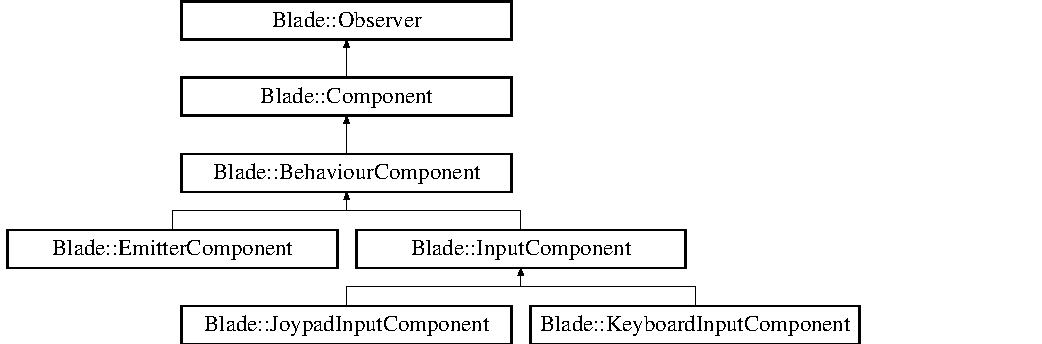
\includegraphics[height=4.597701cm]{class_blade_1_1_behaviour_component}
\end{center}
\end{figure}
\subsection*{Public Member Functions}
\begin{DoxyCompactItemize}
\item 
\hyperlink{class_blade_1_1_behaviour_component_a64cc587591d1b38147ce1dbfb8283f7b}{Behaviour\+Component} (const std\+::string \&type, \hyperlink{class_blade_1_1_entity}{Entity} $\ast$parent)
\begin{DoxyCompactList}\small\item\em \hyperlink{class_blade_1_1_component}{Component} constructor. \end{DoxyCompactList}\item 
\mbox{\Hypertarget{class_blade_1_1_behaviour_component_a2a441fcd82f5b28d588d1eae47a6eaad}\label{class_blade_1_1_behaviour_component_a2a441fcd82f5b28d588d1eae47a6eaad}} 
{\bfseries Behaviour\+Component} (const \hyperlink{class_blade_1_1_behaviour_component}{Behaviour\+Component} \&other)=delete
\item 
\mbox{\Hypertarget{class_blade_1_1_behaviour_component_a7dbee722a714cb89ef12a808d2e48210}\label{class_blade_1_1_behaviour_component_a7dbee722a714cb89ef12a808d2e48210}} 
\hyperlink{class_blade_1_1_behaviour_component}{Behaviour\+Component} \& {\bfseries operator=} (const \hyperlink{class_blade_1_1_behaviour_component}{Behaviour\+Component} \&other)=delete
\item 
virtual void \hyperlink{class_blade_1_1_behaviour_component_a90ec3079534ea1f7225c676881b30c17}{Update} (const float dt, const long time=0) noexcept=0
\begin{DoxyCompactList}\small\item\em Updates the \hyperlink{class_blade_1_1_component}{Component} on each frame. \end{DoxyCompactList}\item 
\mbox{\Hypertarget{class_blade_1_1_behaviour_component_a41aef293d91db79beb3bb99528158ce1}\label{class_blade_1_1_behaviour_component_a41aef293d91db79beb3bb99528158ce1}} 
virtual void \hyperlink{class_blade_1_1_behaviour_component_a41aef293d91db79beb3bb99528158ce1}{Setup} () noexcept=0
\begin{DoxyCompactList}\small\item\em Performs setup actions after the \hyperlink{class_blade_1_1_behaviour_component}{Behaviour\+Component}\textquotesingle{}s creation. \end{DoxyCompactList}\item 
\mbox{\Hypertarget{class_blade_1_1_behaviour_component_a017af86093f174c2b376064f557dcbac}\label{class_blade_1_1_behaviour_component_a017af86093f174c2b376064f557dcbac}} 
virtual void \hyperlink{class_blade_1_1_behaviour_component_a017af86093f174c2b376064f557dcbac}{Teardown} () noexcept=0
\begin{DoxyCompactList}\small\item\em Performs actions before the \hyperlink{class_blade_1_1_behaviour_component}{Behaviour\+Component} is destroyed. \end{DoxyCompactList}\item 
\mbox{\Hypertarget{class_blade_1_1_behaviour_component_a3258a2802f2338855ae2bedb30fe82e7}\label{class_blade_1_1_behaviour_component_a3258a2802f2338855ae2bedb30fe82e7}} 
virtual void {\bfseries On\+Collision} (\hyperlink{class_blade_1_1_entity}{Entity} $\ast$other) noexcept
\end{DoxyCompactItemize}


\subsection{Constructor \& Destructor Documentation}
\mbox{\Hypertarget{class_blade_1_1_behaviour_component_a64cc587591d1b38147ce1dbfb8283f7b}\label{class_blade_1_1_behaviour_component_a64cc587591d1b38147ce1dbfb8283f7b}} 
\index{Blade\+::\+Behaviour\+Component@{Blade\+::\+Behaviour\+Component}!Behaviour\+Component@{Behaviour\+Component}}
\index{Behaviour\+Component@{Behaviour\+Component}!Blade\+::\+Behaviour\+Component@{Blade\+::\+Behaviour\+Component}}
\subsubsection{\texorpdfstring{Behaviour\+Component()}{BehaviourComponent()}}
{\footnotesize\ttfamily Blade\+::\+Behaviour\+Component\+::\+Behaviour\+Component (\begin{DoxyParamCaption}\item[{const std\+::string \&}]{type,  }\item[{\hyperlink{class_blade_1_1_entity}{Entity} $\ast$}]{parent }\end{DoxyParamCaption})}



\hyperlink{class_blade_1_1_component}{Component} constructor. 


\begin{DoxyParams}{Parameters}
{\em type} & The type of the \hyperlink{class_blade_1_1_component}{Component} as a string. \\
\hline
{\em parent} & The \hyperlink{class_blade_1_1_entity}{Entity} the \hyperlink{class_blade_1_1_component}{Component} will be attached to. \\
\hline
\end{DoxyParams}


\subsection{Member Function Documentation}
\mbox{\Hypertarget{class_blade_1_1_behaviour_component_a90ec3079534ea1f7225c676881b30c17}\label{class_blade_1_1_behaviour_component_a90ec3079534ea1f7225c676881b30c17}} 
\index{Blade\+::\+Behaviour\+Component@{Blade\+::\+Behaviour\+Component}!Update@{Update}}
\index{Update@{Update}!Blade\+::\+Behaviour\+Component@{Blade\+::\+Behaviour\+Component}}
\subsubsection{\texorpdfstring{Update()}{Update()}}
{\footnotesize\ttfamily virtual void Blade\+::\+Behaviour\+Component\+::\+Update (\begin{DoxyParamCaption}\item[{const float}]{dt,  }\item[{const long}]{time = {\ttfamily 0} }\end{DoxyParamCaption})\hspace{0.3cm}{\ttfamily [pure virtual]}, {\ttfamily [noexcept]}}



Updates the \hyperlink{class_blade_1_1_component}{Component} on each frame. 


\begin{DoxyParams}{Parameters}
{\em dt} & The time elapsed from the previous frame of the \hyperlink{class_blade_1_1_application}{Application}. \\
\hline
{\em time} & The elapsed time since the start of the \hyperlink{class_blade_1_1_application}{Application}. \\
\hline
\end{DoxyParams}


Implemented in \hyperlink{class_blade_1_1_emitter_component_ac9fe8dec74fec5c575b960cc9d1411ac}{Blade\+::\+Emitter\+Component}, \hyperlink{class_blade_1_1_input_component_aa7869b52200bb0a8c0c304fdf6147098}{Blade\+::\+Input\+Component}, \hyperlink{class_blade_1_1_joypad_input_component_a386bea7c84d17eefa0d40bfa17575e04}{Blade\+::\+Joypad\+Input\+Component}, and \hyperlink{class_blade_1_1_keyboard_input_component_a0945515e8c0513eaa5b536fd4cb2022c}{Blade\+::\+Keyboard\+Input\+Component}.



The documentation for this class was generated from the following files\+:\begin{DoxyCompactItemize}
\item 
include/behaviour\+\_\+component.\+h\item 
src/behaviour\+\_\+component.\+cpp\end{DoxyCompactItemize}

\hypertarget{class_blade_1_1_behaviour_system}{}\section{Blade\+:\+:Behaviour\+System Class Reference}
\label{class_blade_1_1_behaviour_system}\index{Blade\+::\+Behaviour\+System@{Blade\+::\+Behaviour\+System}}


A \hyperlink{class_blade_1_1_system}{System} responsible to process and manage the Behaviour\+Components by calling the Update method on every component.  




{\ttfamily \#include $<$behaviour\+\_\+system.\+h$>$}

Inheritance diagram for Blade\+:\+:Behaviour\+System\+:\begin{figure}[H]
\begin{center}
\leavevmode
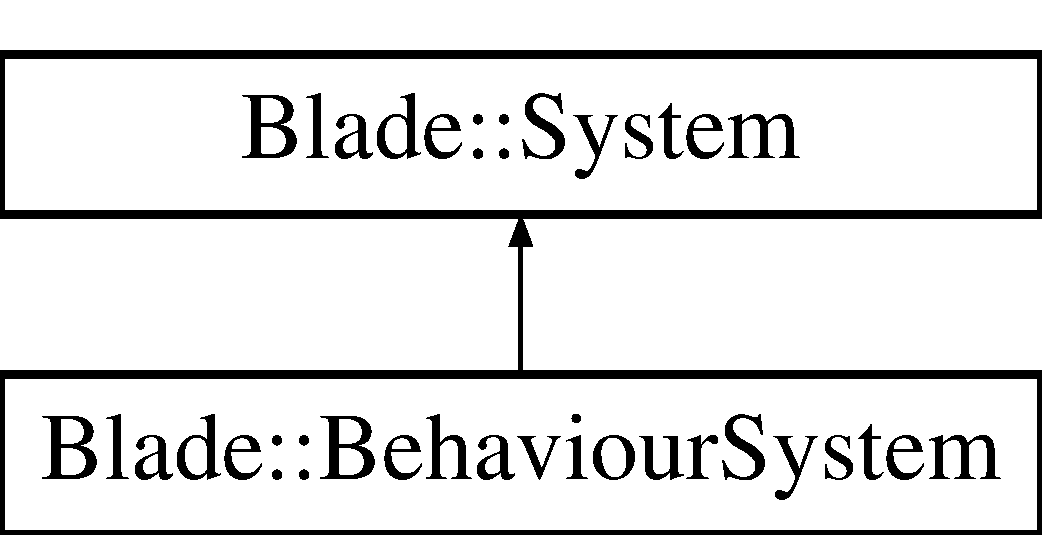
\includegraphics[height=2.000000cm]{class_blade_1_1_behaviour_system}
\end{center}
\end{figure}
\subsection*{Public Member Functions}
\begin{DoxyCompactItemize}
\item 
void \hyperlink{class_blade_1_1_behaviour_system_af233e62b0ee7a43a419069d6de557343}{Process} (float delta\+Time=.\+0f, long time=0) noexcept override
\begin{DoxyCompactList}\small\item\em Processes the \hyperlink{class_blade_1_1_behaviour_component}{Behaviour\+Component}. \end{DoxyCompactList}\item 
bool \hyperlink{class_blade_1_1_behaviour_system_ac4d601f2f88faf7deceb78e01ca8d6be}{Initialize} () noexcept override
\begin{DoxyCompactList}\small\item\em Initializes the \hyperlink{class_blade_1_1_behaviour_system}{Behaviour\+System}. \end{DoxyCompactList}\item 
void \hyperlink{class_blade_1_1_behaviour_system_aafcc2463979e3442abb93c086b4d0cbc}{Register\+Component} (\hyperlink{class_blade_1_1_behaviour_component}{Behaviour\+Component} $\ast$behaviour\+Component) noexcept
\begin{DoxyCompactList}\small\item\em Registers the specified \hyperlink{class_blade_1_1_behaviour_component}{Behaviour\+Component} to the \hyperlink{class_blade_1_1_behaviour_system}{Behaviour\+System}. \end{DoxyCompactList}\item 
void \hyperlink{class_blade_1_1_behaviour_system_a42ca453f54a399c8fb2a1e0010b3d318}{Unregister\+Component} (int id) noexcept
\begin{DoxyCompactList}\small\item\em Unregisters a \hyperlink{class_blade_1_1_behaviour_component}{Behaviour\+Component} from the \hyperlink{class_blade_1_1_behaviour_system}{Behaviour\+System}. \end{DoxyCompactList}\item 
\mbox{\Hypertarget{class_blade_1_1_behaviour_system_ac7400258a6f5c8dd55231beaab6f04f7}\label{class_blade_1_1_behaviour_system_ac7400258a6f5c8dd55231beaab6f04f7}} 
virtual void \hyperlink{class_blade_1_1_behaviour_system_ac7400258a6f5c8dd55231beaab6f04f7}{Setup} () noexcept
\begin{DoxyCompactList}\small\item\em Setup all the \hyperlink{class_blade_1_1_behaviour_component}{Behaviour\+Component} that are currently registered with the \hyperlink{class_blade_1_1_behaviour_system}{Behaviour\+System}. \end{DoxyCompactList}\item 
\mbox{\Hypertarget{class_blade_1_1_behaviour_system_a0082ff7fcadd9224983589b66b027225}\label{class_blade_1_1_behaviour_system_a0082ff7fcadd9224983589b66b027225}} 
virtual void \hyperlink{class_blade_1_1_behaviour_system_a0082ff7fcadd9224983589b66b027225}{Teardown} () noexcept
\begin{DoxyCompactList}\small\item\em Teardown all the \hyperlink{class_blade_1_1_behaviour_component}{Behaviour\+Component} that are currently registered with the \hyperlink{class_blade_1_1_behaviour_system}{Behaviour\+System}. \end{DoxyCompactList}\end{DoxyCompactItemize}


\subsection{Detailed Description}
A \hyperlink{class_blade_1_1_system}{System} responsible to process and manage the Behaviour\+Components by calling the Update method on every component. 

\subsection{Member Function Documentation}
\mbox{\Hypertarget{class_blade_1_1_behaviour_system_ac4d601f2f88faf7deceb78e01ca8d6be}\label{class_blade_1_1_behaviour_system_ac4d601f2f88faf7deceb78e01ca8d6be}} 
\index{Blade\+::\+Behaviour\+System@{Blade\+::\+Behaviour\+System}!Initialize@{Initialize}}
\index{Initialize@{Initialize}!Blade\+::\+Behaviour\+System@{Blade\+::\+Behaviour\+System}}
\subsubsection{\texorpdfstring{Initialize()}{Initialize()}}
{\footnotesize\ttfamily bool Blade\+::\+Behaviour\+System\+::\+Initialize (\begin{DoxyParamCaption}{ }\end{DoxyParamCaption})\hspace{0.3cm}{\ttfamily [override]}, {\ttfamily [virtual]}, {\ttfamily [noexcept]}}



Initializes the \hyperlink{class_blade_1_1_behaviour_system}{Behaviour\+System}. 

\begin{DoxyReturn}{Returns}
T\+R\+UE if initialization is successful, F\+A\+L\+SE otherwise. 
\end{DoxyReturn}


Implements \hyperlink{class_blade_1_1_system_a63fa00af40dc54d093300eff4785f26f}{Blade\+::\+System}.

\mbox{\Hypertarget{class_blade_1_1_behaviour_system_af233e62b0ee7a43a419069d6de557343}\label{class_blade_1_1_behaviour_system_af233e62b0ee7a43a419069d6de557343}} 
\index{Blade\+::\+Behaviour\+System@{Blade\+::\+Behaviour\+System}!Process@{Process}}
\index{Process@{Process}!Blade\+::\+Behaviour\+System@{Blade\+::\+Behaviour\+System}}
\subsubsection{\texorpdfstring{Process()}{Process()}}
{\footnotesize\ttfamily void Blade\+::\+Behaviour\+System\+::\+Process (\begin{DoxyParamCaption}\item[{float}]{delta\+Time = {\ttfamily .0f},  }\item[{long}]{time = {\ttfamily 0} }\end{DoxyParamCaption})\hspace{0.3cm}{\ttfamily [override]}, {\ttfamily [virtual]}, {\ttfamily [noexcept]}}



Processes the \hyperlink{class_blade_1_1_behaviour_component}{Behaviour\+Component}. 


\begin{DoxyParams}{Parameters}
{\em delta\+Time} & The time elapsed from the previous frame of the application. \\
\hline
{\em time} & The time since the application startup \\
\hline
\end{DoxyParams}


Implements \hyperlink{class_blade_1_1_system_a80c186f5f9f8fa4fd317b861853fe6a8}{Blade\+::\+System}.

\mbox{\Hypertarget{class_blade_1_1_behaviour_system_aafcc2463979e3442abb93c086b4d0cbc}\label{class_blade_1_1_behaviour_system_aafcc2463979e3442abb93c086b4d0cbc}} 
\index{Blade\+::\+Behaviour\+System@{Blade\+::\+Behaviour\+System}!Register\+Component@{Register\+Component}}
\index{Register\+Component@{Register\+Component}!Blade\+::\+Behaviour\+System@{Blade\+::\+Behaviour\+System}}
\subsubsection{\texorpdfstring{Register\+Component()}{RegisterComponent()}}
{\footnotesize\ttfamily void Blade\+::\+Behaviour\+System\+::\+Register\+Component (\begin{DoxyParamCaption}\item[{\hyperlink{class_blade_1_1_behaviour_component}{Behaviour\+Component} $\ast$}]{behaviour\+Component }\end{DoxyParamCaption})\hspace{0.3cm}{\ttfamily [noexcept]}}



Registers the specified \hyperlink{class_blade_1_1_behaviour_component}{Behaviour\+Component} to the \hyperlink{class_blade_1_1_behaviour_system}{Behaviour\+System}. 


\begin{DoxyParams}{Parameters}
{\em behaviour\+Component} & The \hyperlink{class_blade_1_1_behaviour_component}{Behaviour\+Component} to be registered to the \hyperlink{class_blade_1_1_behaviour_system}{Behaviour\+System} for processing. \\
\hline
\end{DoxyParams}
\mbox{\Hypertarget{class_blade_1_1_behaviour_system_a42ca453f54a399c8fb2a1e0010b3d318}\label{class_blade_1_1_behaviour_system_a42ca453f54a399c8fb2a1e0010b3d318}} 
\index{Blade\+::\+Behaviour\+System@{Blade\+::\+Behaviour\+System}!Unregister\+Component@{Unregister\+Component}}
\index{Unregister\+Component@{Unregister\+Component}!Blade\+::\+Behaviour\+System@{Blade\+::\+Behaviour\+System}}
\subsubsection{\texorpdfstring{Unregister\+Component()}{UnregisterComponent()}}
{\footnotesize\ttfamily void Blade\+::\+Behaviour\+System\+::\+Unregister\+Component (\begin{DoxyParamCaption}\item[{int}]{id }\end{DoxyParamCaption})\hspace{0.3cm}{\ttfamily [noexcept]}}



Unregisters a \hyperlink{class_blade_1_1_behaviour_component}{Behaviour\+Component} from the \hyperlink{class_blade_1_1_behaviour_system}{Behaviour\+System}. 


\begin{DoxyParams}{Parameters}
{\em id} & The unique id of the \hyperlink{class_blade_1_1_behaviour_component}{Behaviour\+Component} to be unregistered. \\
\hline
\end{DoxyParams}


The documentation for this class was generated from the following files\+:\begin{DoxyCompactItemize}
\item 
include/behaviour\+\_\+system.\+h\item 
src/behaviour\+\_\+sytem.\+cpp\end{DoxyCompactItemize}

\hypertarget{class_blade_1_1_bounding_sphere}{}\section{Blade\+:\+:Bounding\+Sphere Class Reference}
\label{class_blade_1_1_bounding_sphere}\index{Blade\+::\+Bounding\+Sphere@{Blade\+::\+Bounding\+Sphere}}
Inheritance diagram for Blade\+:\+:Bounding\+Sphere\+:\begin{figure}[H]
\begin{center}
\leavevmode
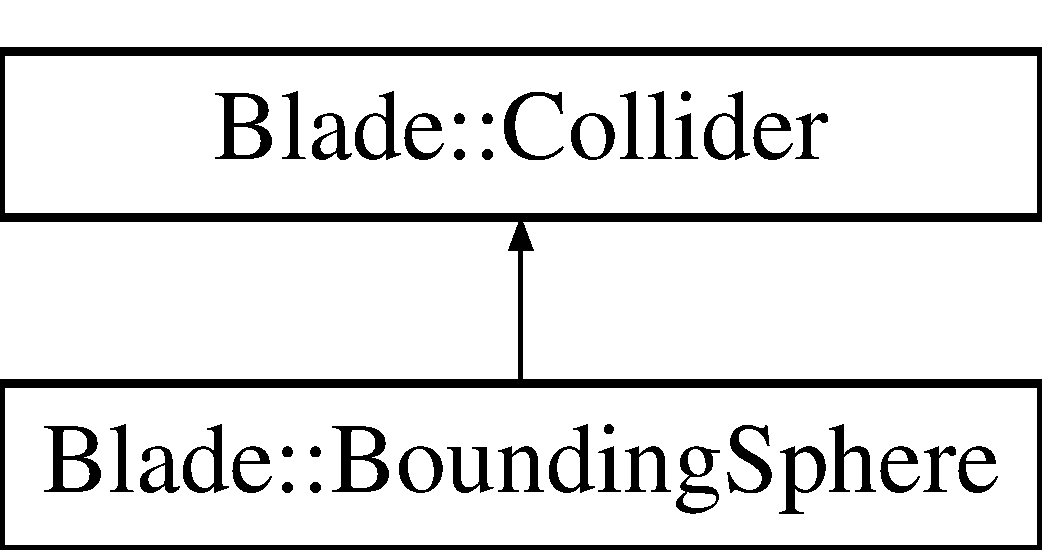
\includegraphics[height=2.000000cm]{class_blade_1_1_bounding_sphere}
\end{center}
\end{figure}
\subsection*{Public Member Functions}
\begin{DoxyCompactItemize}
\item 
\mbox{\Hypertarget{class_blade_1_1_bounding_sphere_aec916c2cd1d3b23b952df9136587bca4}\label{class_blade_1_1_bounding_sphere_aec916c2cd1d3b23b952df9136587bca4}} 
{\bfseries Bounding\+Sphere} (float radius)
\item 
\mbox{\Hypertarget{class_blade_1_1_bounding_sphere_a8d0a579f9489d9e2cc4911b55722df2d}\label{class_blade_1_1_bounding_sphere_a8d0a579f9489d9e2cc4911b55722df2d}} 
bool {\bfseries Collide} (const \hyperlink{class_blade_1_1_collider}{Collider} $\ast$collider, \hyperlink{class_blade_1_1_contact_manifold}{Contact\+Manifold} \&manifold) const noexcept override
\item 
\mbox{\Hypertarget{class_blade_1_1_bounding_sphere_aab2fbff2d3b536952ecb52f2b5f099d1}\label{class_blade_1_1_bounding_sphere_aab2fbff2d3b536952ecb52f2b5f099d1}} 
bool {\bfseries Collide} (const \hyperlink{class_blade_1_1_bounding_sphere}{Bounding\+Sphere} $\ast$bsphere, \hyperlink{class_blade_1_1_contact_manifold}{Contact\+Manifold} \&manifold) const noexcept override
\item 
\mbox{\Hypertarget{class_blade_1_1_bounding_sphere_ab9af5d52b02398b5042daec7af779f33}\label{class_blade_1_1_bounding_sphere_ab9af5d52b02398b5042daec7af779f33}} 
bool {\bfseries Collide} (const \hyperlink{class_blade_1_1_plane_collider}{Plane\+Collider} $\ast$plane, \hyperlink{class_blade_1_1_contact_manifold}{Contact\+Manifold} \&manifold) const noexcept override
\item 
\mbox{\Hypertarget{class_blade_1_1_bounding_sphere_a3c3cf74247377f10b324d36ebd1ca4bd}\label{class_blade_1_1_bounding_sphere_a3c3cf74247377f10b324d36ebd1ca4bd}} 
const float {\bfseries Get\+Radius} () const noexcept
\end{DoxyCompactItemize}


The documentation for this class was generated from the following files\+:\begin{DoxyCompactItemize}
\item 
include/bounding\+\_\+sphere.\+h\item 
src/bounding\+\_\+sphere.\+cpp\end{DoxyCompactItemize}

\hypertarget{class_blade_1_1_camera}{}\section{Blade\+:\+:Camera Class Reference}
\label{class_blade_1_1_camera}\index{Blade\+::\+Camera@{Blade\+::\+Camera}}
Inheritance diagram for Blade\+:\+:Camera\+:\begin{figure}[H]
\begin{center}
\leavevmode
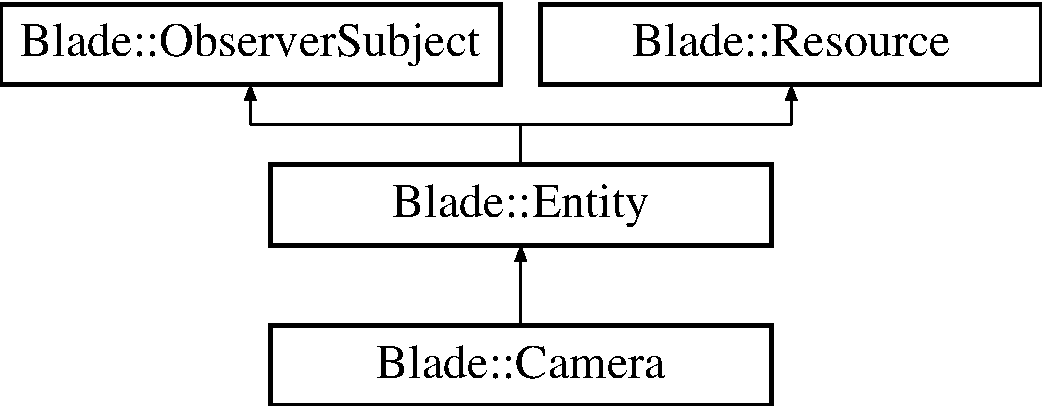
\includegraphics[height=3.000000cm]{class_blade_1_1_camera}
\end{center}
\end{figure}
\subsection*{Public Member Functions}
\begin{DoxyCompactItemize}
\item 
\mbox{\Hypertarget{class_blade_1_1_camera_a84af8fc36ff71a31cfd34861d52e4ac5}\label{class_blade_1_1_camera_a84af8fc36ff71a31cfd34861d52e4ac5}} 
{\bfseries Camera} (const std\+::string \&name, const \hyperlink{struct_blade_1_1_camera_desc}{Camera\+Desc} \&camera\+Description)
\item 
\mbox{\Hypertarget{class_blade_1_1_camera_aa5bf0579c37fb34e5cdec46f1dbcf87b}\label{class_blade_1_1_camera_aa5bf0579c37fb34e5cdec46f1dbcf87b}} 
void {\bfseries Update} (float dt, long time=0) noexcept override
\end{DoxyCompactItemize}


The documentation for this class was generated from the following files\+:\begin{DoxyCompactItemize}
\item 
include/camera.\+h\item 
src/camera.\+cpp\end{DoxyCompactItemize}

\hypertarget{class_blade_1_1_camera_component}{}\section{Blade\+:\+:Camera\+Component Class Reference}
\label{class_blade_1_1_camera_component}\index{Blade\+::\+Camera\+Component@{Blade\+::\+Camera\+Component}}


Represents a \hyperlink{class_blade_1_1_camera_component}{Camera\+Component}. This component contains all the information needed for the view and projection transformations. Managed by the \hyperlink{class_blade_1_1_camera_system}{Camera\+System}.  




{\ttfamily \#include $<$camera\+\_\+component.\+h$>$}

Inheritance diagram for Blade\+:\+:Camera\+Component\+:\begin{figure}[H]
\begin{center}
\leavevmode
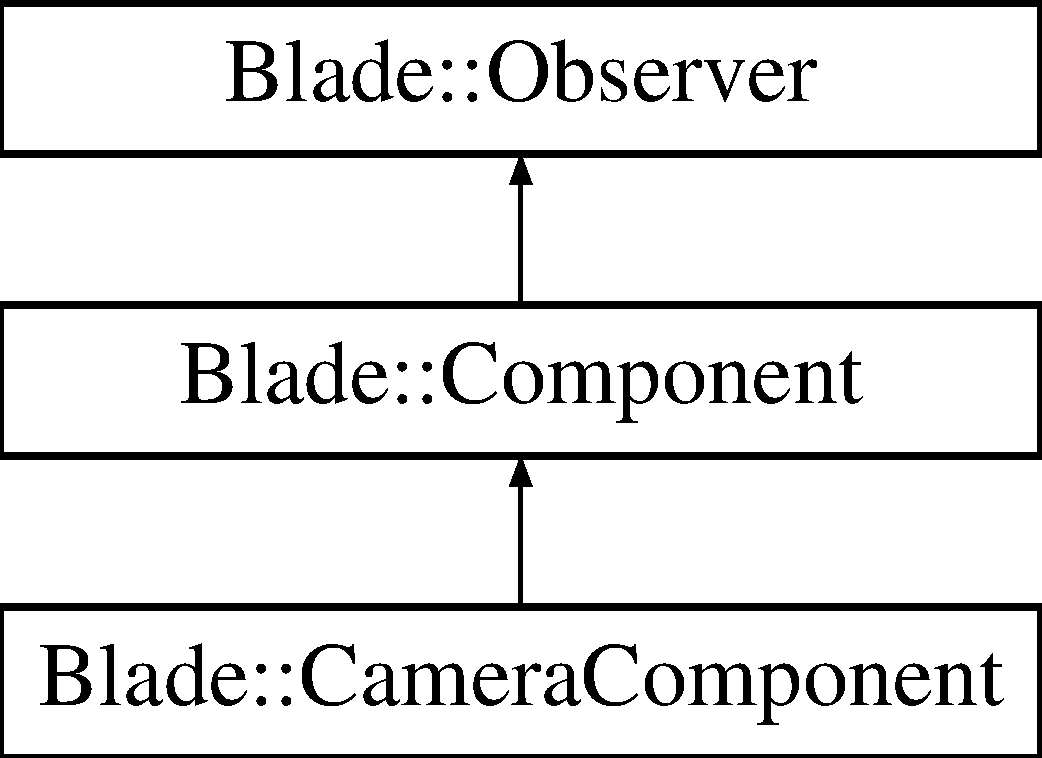
\includegraphics[height=3.000000cm]{class_blade_1_1_camera_component}
\end{center}
\end{figure}
\subsection*{Public Member Functions}
\begin{DoxyCompactItemize}
\item 
\hyperlink{class_blade_1_1_camera_component_a6f66ead0c16432f9840070d40236f099}{Camera\+Component} (\hyperlink{class_blade_1_1_entity}{Entity} $\ast$parent)
\begin{DoxyCompactList}\small\item\em \hyperlink{class_blade_1_1_camera_component}{Camera\+Component}\textquotesingle{}s constructor. \end{DoxyCompactList}\item 
\hyperlink{class_blade_1_1_camera_component_aeb0111051de5e6156dde78ec88cf5afe}{Camera\+Component} (\hyperlink{class_blade_1_1_entity}{Entity} $\ast$parent, float fov, const Viewport \&viewport, float near\+Plane, float far\+Plane)
\item 
\hyperlink{class_blade_1_1_camera_component_ab34dcc016e588bb1b5316e1fd06d9246}{Camera\+Component} (\hyperlink{class_blade_1_1_entity}{Entity} $\ast$parent, float fov, const Viewport \&viewport, const Vec2f \&clipping\+Planes)
\item 
\hyperlink{class_blade_1_1_camera_component_ab0efd673adcb54e7464accfbe80bb612}{$\sim$\+Camera\+Component} ()
\begin{DoxyCompactList}\small\item\em \hyperlink{class_blade_1_1_camera_component}{Camera\+Component}\textquotesingle{}s destructor. \end{DoxyCompactList}\item 
float \hyperlink{class_blade_1_1_camera_component_a74c21029f3b9cc3964e87ef048eebe90}{Get\+Fov} () const noexcept
\begin{DoxyCompactList}\small\item\em Provides the field of view. \end{DoxyCompactList}\item 
void \hyperlink{class_blade_1_1_camera_component_a7d3b2934f93bdb601b177c23e9c1088f}{Set\+Fov} (float fov) noexcept
\begin{DoxyCompactList}\small\item\em Sets the field of view. \end{DoxyCompactList}\item 
const Viewport \& \hyperlink{class_blade_1_1_camera_component_a3ddce5974c61927eb3bb06f2381d780e}{Get\+Viewport} () const noexcept
\begin{DoxyCompactList}\small\item\em Provides the Viewport. \end{DoxyCompactList}\item 
void \hyperlink{class_blade_1_1_camera_component_a9270ae358568b454a760dccaafc1d0c1}{Set\+Viewport} (const Viewport \&viewport) noexcept
\begin{DoxyCompactList}\small\item\em Sets the Viewport. \end{DoxyCompactList}\item 
const Vec2f \& \hyperlink{class_blade_1_1_camera_component_a2eac5f51fbae88dd50ee1077777088c3}{Get\+Clipping\+Planes} () const noexcept
\begin{DoxyCompactList}\small\item\em Provides the clipping planes as a Vec2f. \end{DoxyCompactList}\item 
void \hyperlink{class_blade_1_1_camera_component_aee047bbc83b264db1cea4ebd6445495b}{Set\+Clipping\+Planes} (float near\+Plane, float far\+Plane) noexcept
\begin{DoxyCompactList}\small\item\em Sets the near and the far clipping planes. \end{DoxyCompactList}\item 
void \hyperlink{class_blade_1_1_camera_component_a30416422c87afed3e80a26b14215948f}{Set\+Clipping\+Planes} (const Vec2f \&clipping\+Planes) noexcept
\item 
float \hyperlink{class_blade_1_1_camera_component_a2c1a4dd439d7c27c37e0a15146fe976f}{Get\+Near\+Plane} () const noexcept
\begin{DoxyCompactList}\small\item\em Provides the near clipping plane. \end{DoxyCompactList}\item 
void \hyperlink{class_blade_1_1_camera_component_a808877ff7c5af8c68f900d44ab2e554b}{Set\+Near\+Plane} (float near\+Plane) noexcept
\begin{DoxyCompactList}\small\item\em Sets the near clipping plane. \end{DoxyCompactList}\item 
float \hyperlink{class_blade_1_1_camera_component_ae7f0621c1db163ee530c75775829401b}{Get\+Far\+Plane} () const noexcept
\begin{DoxyCompactList}\small\item\em Provides the far clipping plane. \end{DoxyCompactList}\item 
void \hyperlink{class_blade_1_1_camera_component_a431e7ecb3e2c4302cb1d07c07cb89dc4}{Set\+Far\+Plane} (float far\+Plane) noexcept
\begin{DoxyCompactList}\small\item\em Sets the far clipping plane. \end{DoxyCompactList}\item 
const Mat4f \& \hyperlink{class_blade_1_1_camera_component_a5b8dbf3a13f82da25a0f21d21d92fd99}{Get\+View\+Matrix} () const noexcept
\begin{DoxyCompactList}\small\item\em Provides the view matrix. \end{DoxyCompactList}\item 
void \hyperlink{class_blade_1_1_camera_component_ad1972814c236509dd7fcc9525e068e46}{Set\+View\+Matrix} (const Mat4f \&view\+Matrix) noexcept
\begin{DoxyCompactList}\small\item\em Sets the view matrix. \end{DoxyCompactList}\item 
const Mat4f \& \hyperlink{class_blade_1_1_camera_component_a5d79b698eb708d55538f9b8c045368c6}{Get\+Projection\+Matrix} () const noexcept
\begin{DoxyCompactList}\small\item\em Provides the projection matrix. \end{DoxyCompactList}\item 
\mbox{\Hypertarget{class_blade_1_1_camera_component_a4e8109fb88659b5e08f71ccc3a176fa4}\label{class_blade_1_1_camera_component_a4e8109fb88659b5e08f71ccc3a176fa4}} 
void \hyperlink{class_blade_1_1_camera_component_a4e8109fb88659b5e08f71ccc3a176fa4}{Use\+Perspective\+Projection} () noexcept
\begin{DoxyCompactList}\small\item\em Set the projection matrix with perspective\+LH. \end{DoxyCompactList}\end{DoxyCompactItemize}


\subsection{Detailed Description}
Represents a \hyperlink{class_blade_1_1_camera_component}{Camera\+Component}. This component contains all the information needed for the view and projection transformations. Managed by the \hyperlink{class_blade_1_1_camera_system}{Camera\+System}. 

\subsection{Constructor \& Destructor Documentation}
\mbox{\Hypertarget{class_blade_1_1_camera_component_a6f66ead0c16432f9840070d40236f099}\label{class_blade_1_1_camera_component_a6f66ead0c16432f9840070d40236f099}} 
\index{Blade\+::\+Camera\+Component@{Blade\+::\+Camera\+Component}!Camera\+Component@{Camera\+Component}}
\index{Camera\+Component@{Camera\+Component}!Blade\+::\+Camera\+Component@{Blade\+::\+Camera\+Component}}
\subsubsection{\texorpdfstring{Camera\+Component()}{CameraComponent()}\hspace{0.1cm}{\footnotesize\ttfamily [1/3]}}
{\footnotesize\ttfamily Blade\+::\+Camera\+Component\+::\+Camera\+Component (\begin{DoxyParamCaption}\item[{\hyperlink{class_blade_1_1_entity}{Entity} $\ast$}]{parent }\end{DoxyParamCaption})\hspace{0.3cm}{\ttfamily [explicit]}}



\hyperlink{class_blade_1_1_camera_component}{Camera\+Component}\textquotesingle{}s constructor. 

Registers the component to the \hyperlink{class_blade_1_1_camera_system}{Camera\+System}. 
\begin{DoxyParams}{Parameters}
{\em parent} & The entity the \hyperlink{class_blade_1_1_camera_component}{Camera\+Component} will be attached to. \\
\hline
\end{DoxyParams}
\mbox{\Hypertarget{class_blade_1_1_camera_component_aeb0111051de5e6156dde78ec88cf5afe}\label{class_blade_1_1_camera_component_aeb0111051de5e6156dde78ec88cf5afe}} 
\index{Blade\+::\+Camera\+Component@{Blade\+::\+Camera\+Component}!Camera\+Component@{Camera\+Component}}
\index{Camera\+Component@{Camera\+Component}!Blade\+::\+Camera\+Component@{Blade\+::\+Camera\+Component}}
\subsubsection{\texorpdfstring{Camera\+Component()}{CameraComponent()}\hspace{0.1cm}{\footnotesize\ttfamily [2/3]}}
{\footnotesize\ttfamily Blade\+::\+Camera\+Component\+::\+Camera\+Component (\begin{DoxyParamCaption}\item[{\hyperlink{class_blade_1_1_entity}{Entity} $\ast$}]{parent,  }\item[{float}]{fov,  }\item[{const Viewport \&}]{viewport,  }\item[{float}]{near\+Plane,  }\item[{float}]{far\+Plane }\end{DoxyParamCaption})}

This is an overloaded member function, provided for convenience. It differs from the above function only in what argument(s) it accepts. 
\begin{DoxyParams}{Parameters}
{\em parent} & The entity the \hyperlink{class_blade_1_1_camera_component}{Camera\+Component} will be attached to. \\
\hline
{\em fov} & The field of view. \\
\hline
{\em viewport} & The viewport of the camera. \\
\hline
{\em near\+Plane} & The near clipping plane. \\
\hline
{\em far\+Plane} & The far clipping plane. \\
\hline
\end{DoxyParams}
\mbox{\Hypertarget{class_blade_1_1_camera_component_ab34dcc016e588bb1b5316e1fd06d9246}\label{class_blade_1_1_camera_component_ab34dcc016e588bb1b5316e1fd06d9246}} 
\index{Blade\+::\+Camera\+Component@{Blade\+::\+Camera\+Component}!Camera\+Component@{Camera\+Component}}
\index{Camera\+Component@{Camera\+Component}!Blade\+::\+Camera\+Component@{Blade\+::\+Camera\+Component}}
\subsubsection{\texorpdfstring{Camera\+Component()}{CameraComponent()}\hspace{0.1cm}{\footnotesize\ttfamily [3/3]}}
{\footnotesize\ttfamily Blade\+::\+Camera\+Component\+::\+Camera\+Component (\begin{DoxyParamCaption}\item[{\hyperlink{class_blade_1_1_entity}{Entity} $\ast$}]{parent,  }\item[{float}]{fov,  }\item[{const Viewport \&}]{viewport,  }\item[{const Vec2f \&}]{clipping\+Planes }\end{DoxyParamCaption})}

This is an overloaded member function, provided for convenience. It differs from the above function only in what argument(s) it accepts. 
\begin{DoxyParams}{Parameters}
{\em parent} & The entity the \hyperlink{class_blade_1_1_camera_component}{Camera\+Component} will be attached to. \\
\hline
{\em fov} & The field of view. \\
\hline
{\em viewport} & The viewport of the camera. \\
\hline
{\em clipping\+Planes} & The clipping planes for the projection.\\
\hline
\end{DoxyParams}
clipping\+Planes.\+x -\/ The near clipping plane.

clipping\+Planes.\+y -\/ The far clipping plane. \mbox{\Hypertarget{class_blade_1_1_camera_component_ab0efd673adcb54e7464accfbe80bb612}\label{class_blade_1_1_camera_component_ab0efd673adcb54e7464accfbe80bb612}} 
\index{Blade\+::\+Camera\+Component@{Blade\+::\+Camera\+Component}!````~Camera\+Component@{$\sim$\+Camera\+Component}}
\index{````~Camera\+Component@{$\sim$\+Camera\+Component}!Blade\+::\+Camera\+Component@{Blade\+::\+Camera\+Component}}
\subsubsection{\texorpdfstring{$\sim$\+Camera\+Component()}{~CameraComponent()}}
{\footnotesize\ttfamily Blade\+::\+Camera\+Component\+::$\sim$\+Camera\+Component (\begin{DoxyParamCaption}{ }\end{DoxyParamCaption})}



\hyperlink{class_blade_1_1_camera_component}{Camera\+Component}\textquotesingle{}s destructor. 

Unregisters the component from the \hyperlink{class_blade_1_1_camera_system}{Camera\+System}. 

\subsection{Member Function Documentation}
\mbox{\Hypertarget{class_blade_1_1_camera_component_a2eac5f51fbae88dd50ee1077777088c3}\label{class_blade_1_1_camera_component_a2eac5f51fbae88dd50ee1077777088c3}} 
\index{Blade\+::\+Camera\+Component@{Blade\+::\+Camera\+Component}!Get\+Clipping\+Planes@{Get\+Clipping\+Planes}}
\index{Get\+Clipping\+Planes@{Get\+Clipping\+Planes}!Blade\+::\+Camera\+Component@{Blade\+::\+Camera\+Component}}
\subsubsection{\texorpdfstring{Get\+Clipping\+Planes()}{GetClippingPlanes()}}
{\footnotesize\ttfamily const Vec2f \& Blade\+::\+Camera\+Component\+::\+Get\+Clipping\+Planes (\begin{DoxyParamCaption}{ }\end{DoxyParamCaption}) const\hspace{0.3cm}{\ttfamily [noexcept]}}



Provides the clipping planes as a Vec2f. 

x -\/ The near clipping plane.

y -\/ The far clipping plane. \begin{DoxyReturn}{Returns}
The clipping planes as a Vec2f. 
\end{DoxyReturn}
\mbox{\Hypertarget{class_blade_1_1_camera_component_ae7f0621c1db163ee530c75775829401b}\label{class_blade_1_1_camera_component_ae7f0621c1db163ee530c75775829401b}} 
\index{Blade\+::\+Camera\+Component@{Blade\+::\+Camera\+Component}!Get\+Far\+Plane@{Get\+Far\+Plane}}
\index{Get\+Far\+Plane@{Get\+Far\+Plane}!Blade\+::\+Camera\+Component@{Blade\+::\+Camera\+Component}}
\subsubsection{\texorpdfstring{Get\+Far\+Plane()}{GetFarPlane()}}
{\footnotesize\ttfamily float Blade\+::\+Camera\+Component\+::\+Get\+Far\+Plane (\begin{DoxyParamCaption}{ }\end{DoxyParamCaption}) const\hspace{0.3cm}{\ttfamily [noexcept]}}



Provides the far clipping plane. 

\begin{DoxyReturn}{Returns}
The far clipping plane. 
\end{DoxyReturn}
\mbox{\Hypertarget{class_blade_1_1_camera_component_a74c21029f3b9cc3964e87ef048eebe90}\label{class_blade_1_1_camera_component_a74c21029f3b9cc3964e87ef048eebe90}} 
\index{Blade\+::\+Camera\+Component@{Blade\+::\+Camera\+Component}!Get\+Fov@{Get\+Fov}}
\index{Get\+Fov@{Get\+Fov}!Blade\+::\+Camera\+Component@{Blade\+::\+Camera\+Component}}
\subsubsection{\texorpdfstring{Get\+Fov()}{GetFov()}}
{\footnotesize\ttfamily float Blade\+::\+Camera\+Component\+::\+Get\+Fov (\begin{DoxyParamCaption}{ }\end{DoxyParamCaption}) const\hspace{0.3cm}{\ttfamily [noexcept]}}



Provides the field of view. 

\begin{DoxyReturn}{Returns}
The field of view. 
\end{DoxyReturn}
\mbox{\Hypertarget{class_blade_1_1_camera_component_a2c1a4dd439d7c27c37e0a15146fe976f}\label{class_blade_1_1_camera_component_a2c1a4dd439d7c27c37e0a15146fe976f}} 
\index{Blade\+::\+Camera\+Component@{Blade\+::\+Camera\+Component}!Get\+Near\+Plane@{Get\+Near\+Plane}}
\index{Get\+Near\+Plane@{Get\+Near\+Plane}!Blade\+::\+Camera\+Component@{Blade\+::\+Camera\+Component}}
\subsubsection{\texorpdfstring{Get\+Near\+Plane()}{GetNearPlane()}}
{\footnotesize\ttfamily float Blade\+::\+Camera\+Component\+::\+Get\+Near\+Plane (\begin{DoxyParamCaption}{ }\end{DoxyParamCaption}) const\hspace{0.3cm}{\ttfamily [noexcept]}}



Provides the near clipping plane. 

\begin{DoxyReturn}{Returns}
The near clipping plane. 
\end{DoxyReturn}
\mbox{\Hypertarget{class_blade_1_1_camera_component_a5d79b698eb708d55538f9b8c045368c6}\label{class_blade_1_1_camera_component_a5d79b698eb708d55538f9b8c045368c6}} 
\index{Blade\+::\+Camera\+Component@{Blade\+::\+Camera\+Component}!Get\+Projection\+Matrix@{Get\+Projection\+Matrix}}
\index{Get\+Projection\+Matrix@{Get\+Projection\+Matrix}!Blade\+::\+Camera\+Component@{Blade\+::\+Camera\+Component}}
\subsubsection{\texorpdfstring{Get\+Projection\+Matrix()}{GetProjectionMatrix()}}
{\footnotesize\ttfamily const Mat4f \& Blade\+::\+Camera\+Component\+::\+Get\+Projection\+Matrix (\begin{DoxyParamCaption}{ }\end{DoxyParamCaption}) const\hspace{0.3cm}{\ttfamily [noexcept]}}



Provides the projection matrix. 

\begin{DoxyReturn}{Returns}
The projection matrix. 
\end{DoxyReturn}
\mbox{\Hypertarget{class_blade_1_1_camera_component_a5b8dbf3a13f82da25a0f21d21d92fd99}\label{class_blade_1_1_camera_component_a5b8dbf3a13f82da25a0f21d21d92fd99}} 
\index{Blade\+::\+Camera\+Component@{Blade\+::\+Camera\+Component}!Get\+View\+Matrix@{Get\+View\+Matrix}}
\index{Get\+View\+Matrix@{Get\+View\+Matrix}!Blade\+::\+Camera\+Component@{Blade\+::\+Camera\+Component}}
\subsubsection{\texorpdfstring{Get\+View\+Matrix()}{GetViewMatrix()}}
{\footnotesize\ttfamily const Mat4f \& Blade\+::\+Camera\+Component\+::\+Get\+View\+Matrix (\begin{DoxyParamCaption}{ }\end{DoxyParamCaption}) const\hspace{0.3cm}{\ttfamily [noexcept]}}



Provides the view matrix. 

\begin{DoxyReturn}{Returns}
The view matrix. 
\end{DoxyReturn}
\mbox{\Hypertarget{class_blade_1_1_camera_component_a3ddce5974c61927eb3bb06f2381d780e}\label{class_blade_1_1_camera_component_a3ddce5974c61927eb3bb06f2381d780e}} 
\index{Blade\+::\+Camera\+Component@{Blade\+::\+Camera\+Component}!Get\+Viewport@{Get\+Viewport}}
\index{Get\+Viewport@{Get\+Viewport}!Blade\+::\+Camera\+Component@{Blade\+::\+Camera\+Component}}
\subsubsection{\texorpdfstring{Get\+Viewport()}{GetViewport()}}
{\footnotesize\ttfamily const Viewport \& Blade\+::\+Camera\+Component\+::\+Get\+Viewport (\begin{DoxyParamCaption}{ }\end{DoxyParamCaption}) const\hspace{0.3cm}{\ttfamily [noexcept]}}



Provides the Viewport. 

\begin{DoxyReturn}{Returns}
The Viewport. 
\end{DoxyReturn}
\mbox{\Hypertarget{class_blade_1_1_camera_component_aee047bbc83b264db1cea4ebd6445495b}\label{class_blade_1_1_camera_component_aee047bbc83b264db1cea4ebd6445495b}} 
\index{Blade\+::\+Camera\+Component@{Blade\+::\+Camera\+Component}!Set\+Clipping\+Planes@{Set\+Clipping\+Planes}}
\index{Set\+Clipping\+Planes@{Set\+Clipping\+Planes}!Blade\+::\+Camera\+Component@{Blade\+::\+Camera\+Component}}
\subsubsection{\texorpdfstring{Set\+Clipping\+Planes()}{SetClippingPlanes()}\hspace{0.1cm}{\footnotesize\ttfamily [1/2]}}
{\footnotesize\ttfamily void Blade\+::\+Camera\+Component\+::\+Set\+Clipping\+Planes (\begin{DoxyParamCaption}\item[{float}]{near\+Plane,  }\item[{float}]{far\+Plane }\end{DoxyParamCaption})\hspace{0.3cm}{\ttfamily [noexcept]}}



Sets the near and the far clipping planes. 


\begin{DoxyParams}{Parameters}
{\em near\+Plane} & The near clipping plane. \\
\hline
{\em far\+Plane} & The far clipping plane. \\
\hline
\end{DoxyParams}
\mbox{\Hypertarget{class_blade_1_1_camera_component_a30416422c87afed3e80a26b14215948f}\label{class_blade_1_1_camera_component_a30416422c87afed3e80a26b14215948f}} 
\index{Blade\+::\+Camera\+Component@{Blade\+::\+Camera\+Component}!Set\+Clipping\+Planes@{Set\+Clipping\+Planes}}
\index{Set\+Clipping\+Planes@{Set\+Clipping\+Planes}!Blade\+::\+Camera\+Component@{Blade\+::\+Camera\+Component}}
\subsubsection{\texorpdfstring{Set\+Clipping\+Planes()}{SetClippingPlanes()}\hspace{0.1cm}{\footnotesize\ttfamily [2/2]}}
{\footnotesize\ttfamily void Blade\+::\+Camera\+Component\+::\+Set\+Clipping\+Planes (\begin{DoxyParamCaption}\item[{const Vec2f \&}]{clipping\+Planes }\end{DoxyParamCaption})\hspace{0.3cm}{\ttfamily [noexcept]}}

This is an overloaded member function, provided for convenience. It differs from the above function only in what argument(s) it accepts.

x -\/ The near clipping plane.

y -\/ The far clipping plane. 
\begin{DoxyParams}{Parameters}
{\em clipping\+Planes} & The clipping planes as a Vec2f. \\
\hline
\end{DoxyParams}
\mbox{\Hypertarget{class_blade_1_1_camera_component_a431e7ecb3e2c4302cb1d07c07cb89dc4}\label{class_blade_1_1_camera_component_a431e7ecb3e2c4302cb1d07c07cb89dc4}} 
\index{Blade\+::\+Camera\+Component@{Blade\+::\+Camera\+Component}!Set\+Far\+Plane@{Set\+Far\+Plane}}
\index{Set\+Far\+Plane@{Set\+Far\+Plane}!Blade\+::\+Camera\+Component@{Blade\+::\+Camera\+Component}}
\subsubsection{\texorpdfstring{Set\+Far\+Plane()}{SetFarPlane()}}
{\footnotesize\ttfamily void Blade\+::\+Camera\+Component\+::\+Set\+Far\+Plane (\begin{DoxyParamCaption}\item[{float}]{far\+Plane }\end{DoxyParamCaption})\hspace{0.3cm}{\ttfamily [noexcept]}}



Sets the far clipping plane. 


\begin{DoxyParams}{Parameters}
{\em far\+Plane} & The far clipping plane. \\
\hline
\end{DoxyParams}
\mbox{\Hypertarget{class_blade_1_1_camera_component_a7d3b2934f93bdb601b177c23e9c1088f}\label{class_blade_1_1_camera_component_a7d3b2934f93bdb601b177c23e9c1088f}} 
\index{Blade\+::\+Camera\+Component@{Blade\+::\+Camera\+Component}!Set\+Fov@{Set\+Fov}}
\index{Set\+Fov@{Set\+Fov}!Blade\+::\+Camera\+Component@{Blade\+::\+Camera\+Component}}
\subsubsection{\texorpdfstring{Set\+Fov()}{SetFov()}}
{\footnotesize\ttfamily void Blade\+::\+Camera\+Component\+::\+Set\+Fov (\begin{DoxyParamCaption}\item[{float}]{fov }\end{DoxyParamCaption})\hspace{0.3cm}{\ttfamily [noexcept]}}



Sets the field of view. 


\begin{DoxyParams}{Parameters}
{\em fov} & The field of view. \\
\hline
\end{DoxyParams}
\mbox{\Hypertarget{class_blade_1_1_camera_component_a808877ff7c5af8c68f900d44ab2e554b}\label{class_blade_1_1_camera_component_a808877ff7c5af8c68f900d44ab2e554b}} 
\index{Blade\+::\+Camera\+Component@{Blade\+::\+Camera\+Component}!Set\+Near\+Plane@{Set\+Near\+Plane}}
\index{Set\+Near\+Plane@{Set\+Near\+Plane}!Blade\+::\+Camera\+Component@{Blade\+::\+Camera\+Component}}
\subsubsection{\texorpdfstring{Set\+Near\+Plane()}{SetNearPlane()}}
{\footnotesize\ttfamily void Blade\+::\+Camera\+Component\+::\+Set\+Near\+Plane (\begin{DoxyParamCaption}\item[{float}]{near\+Plane }\end{DoxyParamCaption})\hspace{0.3cm}{\ttfamily [noexcept]}}



Sets the near clipping plane. 


\begin{DoxyParams}{Parameters}
{\em near\+Plane} & The near clipping plane. \\
\hline
\end{DoxyParams}
\mbox{\Hypertarget{class_blade_1_1_camera_component_ad1972814c236509dd7fcc9525e068e46}\label{class_blade_1_1_camera_component_ad1972814c236509dd7fcc9525e068e46}} 
\index{Blade\+::\+Camera\+Component@{Blade\+::\+Camera\+Component}!Set\+View\+Matrix@{Set\+View\+Matrix}}
\index{Set\+View\+Matrix@{Set\+View\+Matrix}!Blade\+::\+Camera\+Component@{Blade\+::\+Camera\+Component}}
\subsubsection{\texorpdfstring{Set\+View\+Matrix()}{SetViewMatrix()}}
{\footnotesize\ttfamily void Blade\+::\+Camera\+Component\+::\+Set\+View\+Matrix (\begin{DoxyParamCaption}\item[{const Mat4f \&}]{view\+Matrix }\end{DoxyParamCaption})\hspace{0.3cm}{\ttfamily [noexcept]}}



Sets the view matrix. 


\begin{DoxyParams}{Parameters}
{\em far\+Plane} & The new view matrix \\
\hline
\end{DoxyParams}
\mbox{\Hypertarget{class_blade_1_1_camera_component_a9270ae358568b454a760dccaafc1d0c1}\label{class_blade_1_1_camera_component_a9270ae358568b454a760dccaafc1d0c1}} 
\index{Blade\+::\+Camera\+Component@{Blade\+::\+Camera\+Component}!Set\+Viewport@{Set\+Viewport}}
\index{Set\+Viewport@{Set\+Viewport}!Blade\+::\+Camera\+Component@{Blade\+::\+Camera\+Component}}
\subsubsection{\texorpdfstring{Set\+Viewport()}{SetViewport()}}
{\footnotesize\ttfamily void Blade\+::\+Camera\+Component\+::\+Set\+Viewport (\begin{DoxyParamCaption}\item[{const Viewport \&}]{viewport }\end{DoxyParamCaption})\hspace{0.3cm}{\ttfamily [noexcept]}}



Sets the Viewport. 


\begin{DoxyParams}{Parameters}
{\em viewport} & The Viewport. \\
\hline
\end{DoxyParams}


The documentation for this class was generated from the following files\+:\begin{DoxyCompactItemize}
\item 
include/camera\+\_\+component.\+h\item 
src/camera\+\_\+component.\+cpp\end{DoxyCompactItemize}

\hypertarget{struct_blade_1_1_camera_desc}{}\section{Blade\+:\+:Camera\+Desc Struct Reference}
\label{struct_blade_1_1_camera_desc}\index{Blade\+::\+Camera\+Desc@{Blade\+::\+Camera\+Desc}}
\subsection*{Public Attributes}
\begin{DoxyCompactItemize}
\item 
\mbox{\Hypertarget{struct_blade_1_1_camera_desc_a82780a72df904a74d2b028a9ed7d2a98}\label{struct_blade_1_1_camera_desc_a82780a72df904a74d2b028a9ed7d2a98}} 
Viewport {\bfseries viewport}
\item 
\mbox{\Hypertarget{struct_blade_1_1_camera_desc_aeb049c5373664a9e0697870a93ea60ef}\label{struct_blade_1_1_camera_desc_aeb049c5373664a9e0697870a93ea60ef}} 
float {\bfseries near\+Plane}
\item 
\mbox{\Hypertarget{struct_blade_1_1_camera_desc_ac779b00cee0a3e1b82ff22099f9f2be6}\label{struct_blade_1_1_camera_desc_ac779b00cee0a3e1b82ff22099f9f2be6}} 
float {\bfseries far\+Plane}
\item 
\mbox{\Hypertarget{struct_blade_1_1_camera_desc_a520f1c4347cc9333350783de975fc499}\label{struct_blade_1_1_camera_desc_a520f1c4347cc9333350783de975fc499}} 
float {\bfseries fov}
\end{DoxyCompactItemize}


The documentation for this struct was generated from the following file\+:\begin{DoxyCompactItemize}
\item 
include/camera.\+h\end{DoxyCompactItemize}

\hypertarget{class_blade_1_1_camera_system}{}\section{Blade\+:\+:Camera\+System Class Reference}
\label{class_blade_1_1_camera_system}\index{Blade\+::\+Camera\+System@{Blade\+::\+Camera\+System}}


A \hyperlink{class_blade_1_1_system}{System} responsible to process and manage the Camera\+Components by swapping the current active camera and providing the current active camera\textquotesingle{}s matrices.  




{\ttfamily \#include $<$camera\+\_\+system.\+h$>$}

Inheritance diagram for Blade\+:\+:Camera\+System\+:\begin{figure}[H]
\begin{center}
\leavevmode
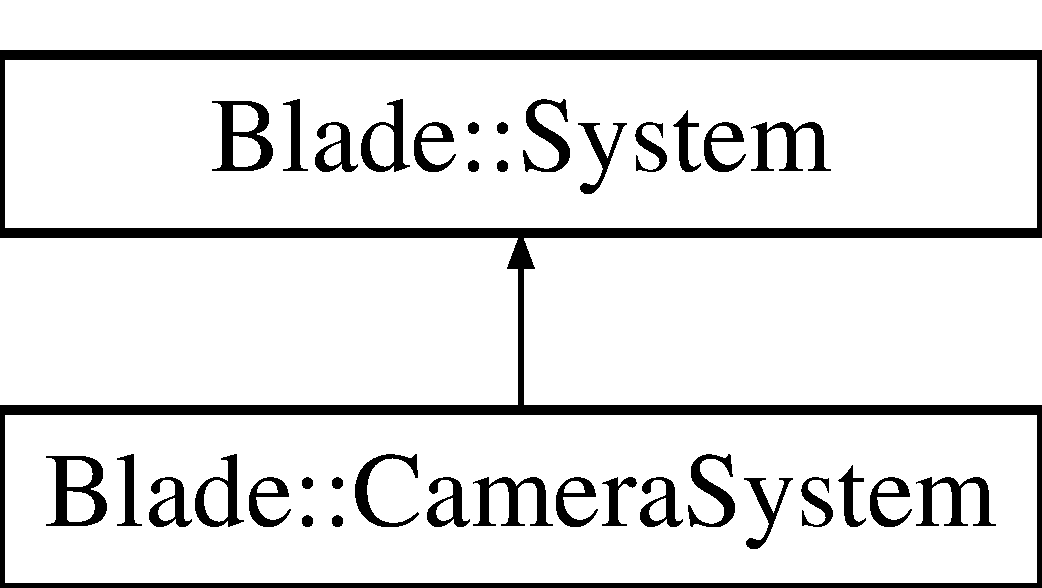
\includegraphics[height=2.000000cm]{class_blade_1_1_camera_system}
\end{center}
\end{figure}
\subsection*{Public Member Functions}
\begin{DoxyCompactItemize}
\item 
void \hyperlink{class_blade_1_1_camera_system_a67a9d2ce6b3f06212dfe882dab6334c6}{Register\+Component} (\hyperlink{class_blade_1_1_camera_component}{Camera\+Component} $\ast$camera\+Component) noexcept
\begin{DoxyCompactList}\small\item\em Registeres the specified \hyperlink{class_blade_1_1_camera_component}{Camera\+Component} to the \hyperlink{class_blade_1_1_camera_system}{Camera\+System}. \end{DoxyCompactList}\item 
void \hyperlink{class_blade_1_1_camera_system_a295fdc352ab2c419940f43610cd06be7}{Unregister\+Component} (int id) noexcept
\begin{DoxyCompactList}\small\item\em Unregisters a \hyperlink{class_blade_1_1_camera_component}{Camera\+Component} from the \hyperlink{class_blade_1_1_camera_system}{Camera\+System}. \end{DoxyCompactList}\item 
void \hyperlink{class_blade_1_1_camera_system_a24ae6ba288185e4c2e915296e2b3a854}{Set\+Active\+Camera} (const std\+::string \&name) noexcept
\begin{DoxyCompactList}\small\item\em Set the camera with the specified name as the active camera. \end{DoxyCompactList}\item 
const Mat4f \& \hyperlink{class_blade_1_1_camera_system_a37ed2fa73706463322331377c6eb8a7f}{Get\+Active\+Camera\+View\+Matrix} () const noexcept
\begin{DoxyCompactList}\small\item\em Provides the active camera\textquotesingle{}s view matrix. \end{DoxyCompactList}\item 
const Mat4f \& \hyperlink{class_blade_1_1_camera_system_ab70602bec3fdc6fbfe26d90a789d40bc}{Get\+Active\+Camera\+Projection\+Matrtix} () const noexcept
\begin{DoxyCompactList}\small\item\em Provides the active camera\textquotesingle{}s projection matrix. \end{DoxyCompactList}\item 
const Viewport \& \hyperlink{class_blade_1_1_camera_system_aff681b50b700fb56721fcd844c961e3f}{Get\+Active\+Camera\+Viewport} () const noexcept
\begin{DoxyCompactList}\small\item\em Provides the active camera\textquotesingle{}s Viewport. \end{DoxyCompactList}\item 
\hyperlink{class_blade_1_1_camera_component}{Camera\+Component} $\ast$ \hyperlink{class_blade_1_1_camera_system_aad7510843cd3b0ab6beeff854c96f6ad}{Get\+Active\+Camera} () const noexcept
\begin{DoxyCompactList}\small\item\em Provides the active camera\textquotesingle{}s \hyperlink{class_blade_1_1_camera_component}{Camera\+Component}. \end{DoxyCompactList}\item 
\hyperlink{class_blade_1_1_camera_component}{Camera\+Component} $\ast$ \hyperlink{class_blade_1_1_camera_system_aa6fcc138bf6920081fb7a36ddf362894}{Get\+Camera} (const std\+::string \&name) noexcept
\begin{DoxyCompactList}\small\item\em Provides the \hyperlink{class_blade_1_1_camera_component}{Camera\+Component} of the camera with the specified name. \end{DoxyCompactList}\end{DoxyCompactItemize}


\subsection{Detailed Description}
A \hyperlink{class_blade_1_1_system}{System} responsible to process and manage the Camera\+Components by swapping the current active camera and providing the current active camera\textquotesingle{}s matrices. 

\subsection{Member Function Documentation}
\mbox{\Hypertarget{class_blade_1_1_camera_system_aad7510843cd3b0ab6beeff854c96f6ad}\label{class_blade_1_1_camera_system_aad7510843cd3b0ab6beeff854c96f6ad}} 
\index{Blade\+::\+Camera\+System@{Blade\+::\+Camera\+System}!Get\+Active\+Camera@{Get\+Active\+Camera}}
\index{Get\+Active\+Camera@{Get\+Active\+Camera}!Blade\+::\+Camera\+System@{Blade\+::\+Camera\+System}}
\subsubsection{\texorpdfstring{Get\+Active\+Camera()}{GetActiveCamera()}}
{\footnotesize\ttfamily \hyperlink{class_blade_1_1_camera_component}{Camera\+Component} $\ast$ Blade\+::\+Camera\+System\+::\+Get\+Active\+Camera (\begin{DoxyParamCaption}{ }\end{DoxyParamCaption}) const\hspace{0.3cm}{\ttfamily [noexcept]}}



Provides the active camera\textquotesingle{}s \hyperlink{class_blade_1_1_camera_component}{Camera\+Component}. 

\begin{DoxyReturn}{Returns}
The active camera\textquotesingle{}s \hyperlink{class_blade_1_1_camera_component}{Camera\+Component}. 
\end{DoxyReturn}
\mbox{\Hypertarget{class_blade_1_1_camera_system_ab70602bec3fdc6fbfe26d90a789d40bc}\label{class_blade_1_1_camera_system_ab70602bec3fdc6fbfe26d90a789d40bc}} 
\index{Blade\+::\+Camera\+System@{Blade\+::\+Camera\+System}!Get\+Active\+Camera\+Projection\+Matrtix@{Get\+Active\+Camera\+Projection\+Matrtix}}
\index{Get\+Active\+Camera\+Projection\+Matrtix@{Get\+Active\+Camera\+Projection\+Matrtix}!Blade\+::\+Camera\+System@{Blade\+::\+Camera\+System}}
\subsubsection{\texorpdfstring{Get\+Active\+Camera\+Projection\+Matrtix()}{GetActiveCameraProjectionMatrtix()}}
{\footnotesize\ttfamily const Mat4f \& Blade\+::\+Camera\+System\+::\+Get\+Active\+Camera\+Projection\+Matrtix (\begin{DoxyParamCaption}{ }\end{DoxyParamCaption}) const\hspace{0.3cm}{\ttfamily [noexcept]}}



Provides the active camera\textquotesingle{}s projection matrix. 

\begin{DoxyReturn}{Returns}
The active camera\textquotesingle{}s projection matrix. 
\end{DoxyReturn}
\mbox{\Hypertarget{class_blade_1_1_camera_system_a37ed2fa73706463322331377c6eb8a7f}\label{class_blade_1_1_camera_system_a37ed2fa73706463322331377c6eb8a7f}} 
\index{Blade\+::\+Camera\+System@{Blade\+::\+Camera\+System}!Get\+Active\+Camera\+View\+Matrix@{Get\+Active\+Camera\+View\+Matrix}}
\index{Get\+Active\+Camera\+View\+Matrix@{Get\+Active\+Camera\+View\+Matrix}!Blade\+::\+Camera\+System@{Blade\+::\+Camera\+System}}
\subsubsection{\texorpdfstring{Get\+Active\+Camera\+View\+Matrix()}{GetActiveCameraViewMatrix()}}
{\footnotesize\ttfamily const Mat4f \& Blade\+::\+Camera\+System\+::\+Get\+Active\+Camera\+View\+Matrix (\begin{DoxyParamCaption}{ }\end{DoxyParamCaption}) const\hspace{0.3cm}{\ttfamily [noexcept]}}



Provides the active camera\textquotesingle{}s view matrix. 

\begin{DoxyReturn}{Returns}
The active camera\textquotesingle{}s view matrix. 
\end{DoxyReturn}
\mbox{\Hypertarget{class_blade_1_1_camera_system_aff681b50b700fb56721fcd844c961e3f}\label{class_blade_1_1_camera_system_aff681b50b700fb56721fcd844c961e3f}} 
\index{Blade\+::\+Camera\+System@{Blade\+::\+Camera\+System}!Get\+Active\+Camera\+Viewport@{Get\+Active\+Camera\+Viewport}}
\index{Get\+Active\+Camera\+Viewport@{Get\+Active\+Camera\+Viewport}!Blade\+::\+Camera\+System@{Blade\+::\+Camera\+System}}
\subsubsection{\texorpdfstring{Get\+Active\+Camera\+Viewport()}{GetActiveCameraViewport()}}
{\footnotesize\ttfamily const Viewport \& Blade\+::\+Camera\+System\+::\+Get\+Active\+Camera\+Viewport (\begin{DoxyParamCaption}{ }\end{DoxyParamCaption}) const\hspace{0.3cm}{\ttfamily [noexcept]}}



Provides the active camera\textquotesingle{}s Viewport. 

\begin{DoxyReturn}{Returns}
The active camera\textquotesingle{}s Viewport. 
\end{DoxyReturn}
\mbox{\Hypertarget{class_blade_1_1_camera_system_aa6fcc138bf6920081fb7a36ddf362894}\label{class_blade_1_1_camera_system_aa6fcc138bf6920081fb7a36ddf362894}} 
\index{Blade\+::\+Camera\+System@{Blade\+::\+Camera\+System}!Get\+Camera@{Get\+Camera}}
\index{Get\+Camera@{Get\+Camera}!Blade\+::\+Camera\+System@{Blade\+::\+Camera\+System}}
\subsubsection{\texorpdfstring{Get\+Camera()}{GetCamera()}}
{\footnotesize\ttfamily \hyperlink{class_blade_1_1_camera_component}{Camera\+Component} $\ast$ Blade\+::\+Camera\+System\+::\+Get\+Camera (\begin{DoxyParamCaption}\item[{const std\+::string \&}]{name }\end{DoxyParamCaption})\hspace{0.3cm}{\ttfamily [noexcept]}}



Provides the \hyperlink{class_blade_1_1_camera_component}{Camera\+Component} of the camera with the specified name. 


\begin{DoxyParams}{Parameters}
{\em name} & The name of the camera to be returned. \\
\hline
\end{DoxyParams}
\begin{DoxyReturn}{Returns}
The \hyperlink{class_blade_1_1_camera_component}{Camera\+Component} of the camera with the specified name. 
\end{DoxyReturn}
\mbox{\Hypertarget{class_blade_1_1_camera_system_a67a9d2ce6b3f06212dfe882dab6334c6}\label{class_blade_1_1_camera_system_a67a9d2ce6b3f06212dfe882dab6334c6}} 
\index{Blade\+::\+Camera\+System@{Blade\+::\+Camera\+System}!Register\+Component@{Register\+Component}}
\index{Register\+Component@{Register\+Component}!Blade\+::\+Camera\+System@{Blade\+::\+Camera\+System}}
\subsubsection{\texorpdfstring{Register\+Component()}{RegisterComponent()}}
{\footnotesize\ttfamily void Blade\+::\+Camera\+System\+::\+Register\+Component (\begin{DoxyParamCaption}\item[{\hyperlink{class_blade_1_1_camera_component}{Camera\+Component} $\ast$}]{camera\+Component }\end{DoxyParamCaption})\hspace{0.3cm}{\ttfamily [noexcept]}}



Registeres the specified \hyperlink{class_blade_1_1_camera_component}{Camera\+Component} to the \hyperlink{class_blade_1_1_camera_system}{Camera\+System}. 


\begin{DoxyParams}{Parameters}
{\em camera\+Component} & The \hyperlink{class_blade_1_1_camera_component}{Camera\+Component} to be registered to the Camera\+Sytstem for processing. \\
\hline
\end{DoxyParams}
\mbox{\Hypertarget{class_blade_1_1_camera_system_a24ae6ba288185e4c2e915296e2b3a854}\label{class_blade_1_1_camera_system_a24ae6ba288185e4c2e915296e2b3a854}} 
\index{Blade\+::\+Camera\+System@{Blade\+::\+Camera\+System}!Set\+Active\+Camera@{Set\+Active\+Camera}}
\index{Set\+Active\+Camera@{Set\+Active\+Camera}!Blade\+::\+Camera\+System@{Blade\+::\+Camera\+System}}
\subsubsection{\texorpdfstring{Set\+Active\+Camera()}{SetActiveCamera()}}
{\footnotesize\ttfamily void Blade\+::\+Camera\+System\+::\+Set\+Active\+Camera (\begin{DoxyParamCaption}\item[{const std\+::string \&}]{name }\end{DoxyParamCaption})\hspace{0.3cm}{\ttfamily [noexcept]}}



Set the camera with the specified name as the active camera. 


\begin{DoxyParams}{Parameters}
{\em name} & The name of the camera to be set as active. \\
\hline
\end{DoxyParams}
\mbox{\Hypertarget{class_blade_1_1_camera_system_a295fdc352ab2c419940f43610cd06be7}\label{class_blade_1_1_camera_system_a295fdc352ab2c419940f43610cd06be7}} 
\index{Blade\+::\+Camera\+System@{Blade\+::\+Camera\+System}!Unregister\+Component@{Unregister\+Component}}
\index{Unregister\+Component@{Unregister\+Component}!Blade\+::\+Camera\+System@{Blade\+::\+Camera\+System}}
\subsubsection{\texorpdfstring{Unregister\+Component()}{UnregisterComponent()}}
{\footnotesize\ttfamily void Blade\+::\+Camera\+System\+::\+Unregister\+Component (\begin{DoxyParamCaption}\item[{int}]{id }\end{DoxyParamCaption})\hspace{0.3cm}{\ttfamily [noexcept]}}



Unregisters a \hyperlink{class_blade_1_1_camera_component}{Camera\+Component} from the \hyperlink{class_blade_1_1_camera_system}{Camera\+System}. 


\begin{DoxyParams}{Parameters}
{\em id} & The unique id of the \hyperlink{class_blade_1_1_camera_component}{Camera\+Component} to be unregistered. \\
\hline
\end{DoxyParams}


The documentation for this class was generated from the following files\+:\begin{DoxyCompactItemize}
\item 
include/camera\+\_\+system.\+h\item 
src/camera\+\_\+system.\+cpp\end{DoxyCompactItemize}

\hypertarget{class_blade_1_1_collider}{}\section{Blade\+:\+:Collider Class Reference}
\label{class_blade_1_1_collider}\index{Blade\+::\+Collider@{Blade\+::\+Collider}}
Inheritance diagram for Blade\+:\+:Collider\+:\begin{figure}[H]
\begin{center}
\leavevmode
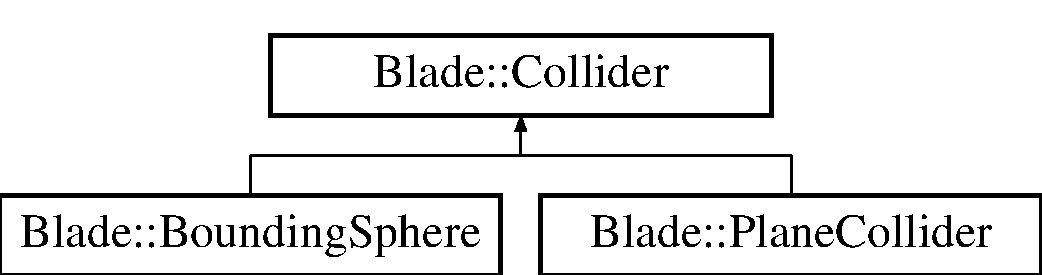
\includegraphics[height=2.000000cm]{class_blade_1_1_collider}
\end{center}
\end{figure}
\subsection*{Public Member Functions}
\begin{DoxyCompactItemize}
\item 
\mbox{\Hypertarget{class_blade_1_1_collider_ae938f3f578348c063651bd51c1050f17}\label{class_blade_1_1_collider_ae938f3f578348c063651bd51c1050f17}} 
virtual bool {\bfseries Collide} (const \hyperlink{class_blade_1_1_collider}{Collider} $\ast$collider, \hyperlink{class_blade_1_1_contact_manifold}{Contact\+Manifold} \&manifold) const noexcept=0
\item 
\mbox{\Hypertarget{class_blade_1_1_collider_a40861d157496f41072a290a3da498fc9}\label{class_blade_1_1_collider_a40861d157496f41072a290a3da498fc9}} 
virtual bool {\bfseries Collide} (const \hyperlink{class_blade_1_1_bounding_sphere}{Bounding\+Sphere} $\ast$bsphere, \hyperlink{class_blade_1_1_contact_manifold}{Contact\+Manifold} \&manifold) const noexcept=0
\item 
\mbox{\Hypertarget{class_blade_1_1_collider_ab5988bae63836308e67e26c5a0f1f62d}\label{class_blade_1_1_collider_ab5988bae63836308e67e26c5a0f1f62d}} 
virtual bool {\bfseries Collide} (const \hyperlink{class_blade_1_1_plane_collider}{Plane\+Collider} $\ast$plane, \hyperlink{class_blade_1_1_contact_manifold}{Contact\+Manifold} \&manifold) const noexcept=0
\item 
\mbox{\Hypertarget{class_blade_1_1_collider_a8e00c2409092ee0f458d134636d90c60}\label{class_blade_1_1_collider_a8e00c2409092ee0f458d134636d90c60}} 
\hyperlink{class_blade_1_1_collider_component}{Collider\+Component} $\ast$ {\bfseries Get\+Collider\+Component} () const noexcept
\item 
\mbox{\Hypertarget{class_blade_1_1_collider_affd7dabd926a2e2b3cf857f434976769}\label{class_blade_1_1_collider_affd7dabd926a2e2b3cf857f434976769}} 
void {\bfseries Set\+Parent} (\hyperlink{class_blade_1_1_collider_component}{Collider\+Component} $\ast$cc) noexcept
\end{DoxyCompactItemize}


The documentation for this class was generated from the following file\+:\begin{DoxyCompactItemize}
\item 
include/collider.\+h\end{DoxyCompactItemize}

\hypertarget{class_blade_1_1_collider_component}{}\section{Blade\+:\+:Collider\+Component Class Reference}
\label{class_blade_1_1_collider_component}\index{Blade\+::\+Collider\+Component@{Blade\+::\+Collider\+Component}}
Inheritance diagram for Blade\+:\+:Collider\+Component\+:\begin{figure}[H]
\begin{center}
\leavevmode
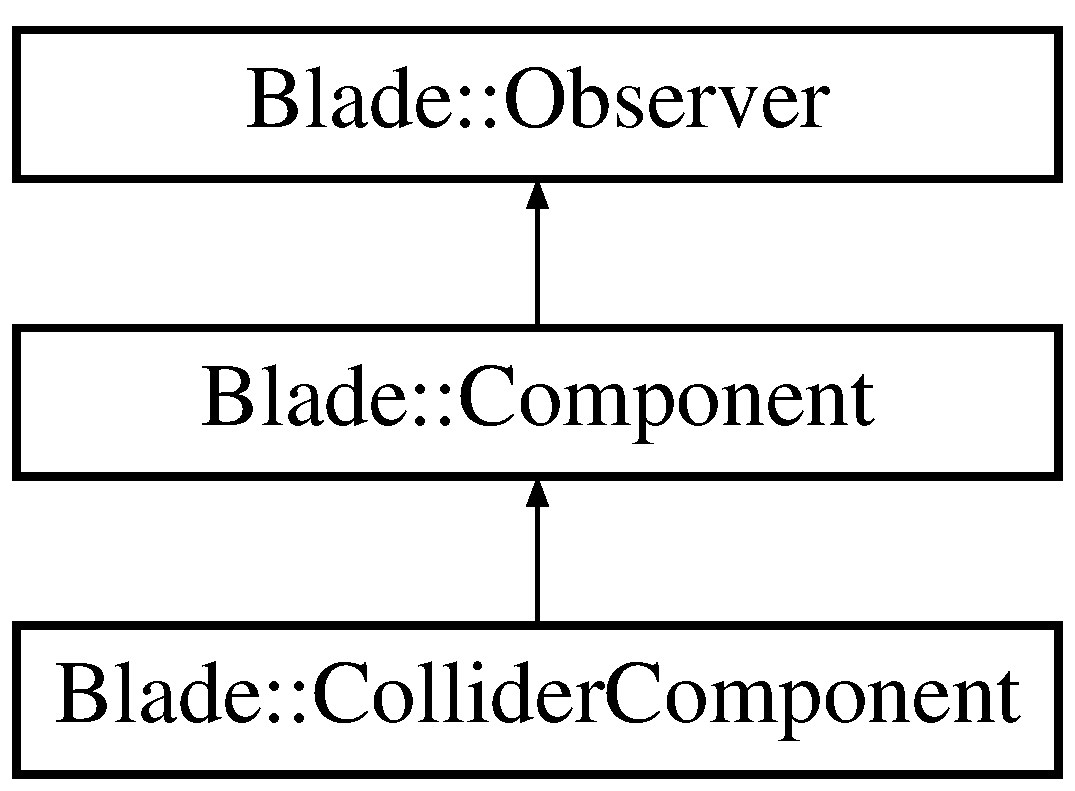
\includegraphics[height=3.000000cm]{class_blade_1_1_collider_component}
\end{center}
\end{figure}
\subsection*{Public Member Functions}
\begin{DoxyCompactItemize}
\item 
\mbox{\Hypertarget{class_blade_1_1_collider_component_a00da11e1d8b4035d389d738dd33d2331}\label{class_blade_1_1_collider_component_a00da11e1d8b4035d389d738dd33d2331}} 
{\bfseries Collider\+Component} (\hyperlink{class_blade_1_1_entity}{Entity} $\ast$parent, std\+::unique\+\_\+ptr$<$ \hyperlink{class_blade_1_1_collider}{Collider} $>$ collider)
\item 
\mbox{\Hypertarget{class_blade_1_1_collider_component_a66647067a95a32e362ade6c7f61718b6}\label{class_blade_1_1_collider_component_a66647067a95a32e362ade6c7f61718b6}} 
{\bfseries Collider\+Component} (\hyperlink{class_blade_1_1_collider_component}{Collider\+Component} \&)=delete
\item 
\mbox{\Hypertarget{class_blade_1_1_collider_component_a761be8a3fcb1f25bf834006ba4903c73}\label{class_blade_1_1_collider_component_a761be8a3fcb1f25bf834006ba4903c73}} 
\hyperlink{class_blade_1_1_collider_component}{Collider\+Component} \& {\bfseries operator=} (\hyperlink{class_blade_1_1_collider_component}{Collider\+Component} \&)=delete
\item 
\mbox{\Hypertarget{class_blade_1_1_collider_component_a963645ea85df676a53331ee73fb8c1be}\label{class_blade_1_1_collider_component_a963645ea85df676a53331ee73fb8c1be}} 
void {\bfseries Set\+Collider} (std\+::unique\+\_\+ptr$<$ \hyperlink{class_blade_1_1_collider}{Collider} $>$ collider) noexcept
\item 
\mbox{\Hypertarget{class_blade_1_1_collider_component_a12849cf36520371d006e008eed2afab5}\label{class_blade_1_1_collider_component_a12849cf36520371d006e008eed2afab5}} 
\hyperlink{class_blade_1_1_collider}{Collider} $\ast$ {\bfseries Get\+Collider} () const noexcept
\item 
\mbox{\Hypertarget{class_blade_1_1_collider_component_a3bad0a0380c3738311ccce2471ff2bfc}\label{class_blade_1_1_collider_component_a3bad0a0380c3738311ccce2471ff2bfc}} 
bool {\bfseries Is\+Active} () const noexcept
\item 
\mbox{\Hypertarget{class_blade_1_1_collider_component_a87d47d39580a943564fdc5dc8b909efa}\label{class_blade_1_1_collider_component_a87d47d39580a943564fdc5dc8b909efa}} 
void {\bfseries Set\+Collision\+Response\+Flag} (bool flag) noexcept
\item 
\mbox{\Hypertarget{class_blade_1_1_collider_component_a02858894d052b92d17224a55c9be5934}\label{class_blade_1_1_collider_component_a02858894d052b92d17224a55c9be5934}} 
void {\bfseries Add\+Listener} (\hyperlink{class_blade_1_1_behaviour_component}{Behaviour\+Component} $\ast$listener) noexcept
\item 
\mbox{\Hypertarget{class_blade_1_1_collider_component_ad7507d81243c8dd2933bebb8962d69b2}\label{class_blade_1_1_collider_component_ad7507d81243c8dd2933bebb8962d69b2}} 
void {\bfseries Notify\+Collision\+Listeners} (\hyperlink{class_blade_1_1_entity}{Entity} $\ast$entity) noexcept
\end{DoxyCompactItemize}


The documentation for this class was generated from the following files\+:\begin{DoxyCompactItemize}
\item 
include/collider\+\_\+component.\+h\item 
src/collider\+\_\+component.\+cpp\end{DoxyCompactItemize}

\hypertarget{class_blade_1_1_command}{}\section{Blade\+:\+:Command Class Reference}
\label{class_blade_1_1_command}\index{Blade\+::\+Command@{Blade\+::\+Command}}


\hyperlink{class_blade_1_1_command}{Command} pattern class.\+Encapsulate a request as an object, thereby letting users parameterize clients with different requests,queue or log requests, and support undo able operations.  




{\ttfamily \#include $<$command.\+h$>$}

\subsection*{Public Member Functions}
\begin{DoxyCompactItemize}
\item 
\hyperlink{class_blade_1_1_command_ad2d8d0d0f38cb5e3142ae4876e041946}{Command} (bool online=false)
\begin{DoxyCompactList}\small\item\em Constructor of a command. \end{DoxyCompactList}\item 
virtual void \hyperlink{class_blade_1_1_command_a9110a3b9580a9e820c9318cf96bb6c41}{Execute} (\hyperlink{class_blade_1_1_entity}{Entity} $\ast$entity, const float dt)=0
\begin{DoxyCompactList}\small\item\em Execute method of the command. \end{DoxyCompactList}\end{DoxyCompactItemize}
\subsection*{Protected Attributes}
\begin{DoxyCompactItemize}
\item 
\mbox{\Hypertarget{class_blade_1_1_command_ab473805a51a806fc54204078604d4550}\label{class_blade_1_1_command_ab473805a51a806fc54204078604d4550}} 
bool {\bfseries m\+\_\+\+Online}
\end{DoxyCompactItemize}


\subsection{Detailed Description}
\hyperlink{class_blade_1_1_command}{Command} pattern class.\+Encapsulate a request as an object, thereby letting users parameterize clients with different requests,queue or log requests, and support undo able operations. 

\subsection{Constructor \& Destructor Documentation}
\mbox{\Hypertarget{class_blade_1_1_command_ad2d8d0d0f38cb5e3142ae4876e041946}\label{class_blade_1_1_command_ad2d8d0d0f38cb5e3142ae4876e041946}} 
\index{Blade\+::\+Command@{Blade\+::\+Command}!Command@{Command}}
\index{Command@{Command}!Blade\+::\+Command@{Blade\+::\+Command}}
\subsubsection{\texorpdfstring{Command()}{Command()}}
{\footnotesize\ttfamily Blade\+::\+Command\+::\+Command (\begin{DoxyParamCaption}\item[{bool}]{online = {\ttfamily false} }\end{DoxyParamCaption})\hspace{0.3cm}{\ttfamily [inline]}}



Constructor of a command. 


\begin{DoxyParams}{Parameters}
{\em online} & T\+R\+UE if the command has to adopt a special treatment for online functionalities (sending messages etc). \\
\hline
\end{DoxyParams}


\subsection{Member Function Documentation}
\mbox{\Hypertarget{class_blade_1_1_command_a9110a3b9580a9e820c9318cf96bb6c41}\label{class_blade_1_1_command_a9110a3b9580a9e820c9318cf96bb6c41}} 
\index{Blade\+::\+Command@{Blade\+::\+Command}!Execute@{Execute}}
\index{Execute@{Execute}!Blade\+::\+Command@{Blade\+::\+Command}}
\subsubsection{\texorpdfstring{Execute()}{Execute()}}
{\footnotesize\ttfamily virtual void Blade\+::\+Command\+::\+Execute (\begin{DoxyParamCaption}\item[{\hyperlink{class_blade_1_1_entity}{Entity} $\ast$}]{entity,  }\item[{const float}]{dt }\end{DoxyParamCaption})\hspace{0.3cm}{\ttfamily [pure virtual]}}



Execute method of the command. 


\begin{DoxyParams}{Parameters}
{\em entity} & the entity that performs the action \\
\hline
{\em dt} & the delta time. \\
\hline
\end{DoxyParams}


The documentation for this class was generated from the following file\+:\begin{DoxyCompactItemize}
\item 
include/command.\+h\end{DoxyCompactItemize}

\hypertarget{class_blade_1_1_component}{}\section{Blade\+:\+:Component Class Reference}
\label{class_blade_1_1_component}\index{Blade\+::\+Component@{Blade\+::\+Component}}


Base \hyperlink{class_blade_1_1_component}{Component} class of the engine. All the components of the engine derive from this class. Compoment inherits from the \hyperlink{class_blade_1_1_observer}{Observer} class so it can register and receive specific messages.  




{\ttfamily \#include $<$component.\+h$>$}

Inheritance diagram for Blade\+:\+:Component\+:\begin{figure}[H]
\begin{center}
\leavevmode
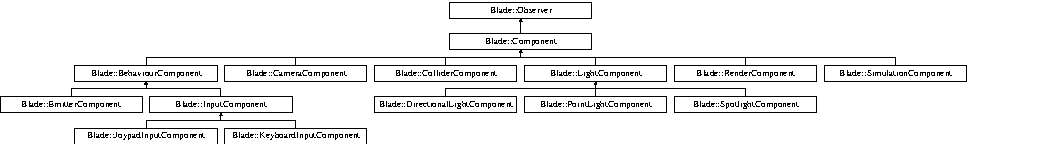
\includegraphics[height=1.913875cm]{class_blade_1_1_component}
\end{center}
\end{figure}
\subsection*{Public Member Functions}
\begin{DoxyCompactItemize}
\item 
\hyperlink{class_blade_1_1_component_a9afd6318db086a2fa6bfdbbbc009ef85}{Component} (const std\+::string \&type, \hyperlink{class_blade_1_1_entity}{Entity} $\ast$parent)
\begin{DoxyCompactList}\small\item\em \hyperlink{class_blade_1_1_component}{Component} constructor. \end{DoxyCompactList}\item 
\mbox{\Hypertarget{class_blade_1_1_component_a8f82f850d6487c061112513171a3ebe2}\label{class_blade_1_1_component_a8f82f850d6487c061112513171a3ebe2}} 
{\bfseries Component} (const \hyperlink{class_blade_1_1_component}{Component} \&other)=delete
\item 
\mbox{\Hypertarget{class_blade_1_1_component_abbed7271dc6e5d937a6a1fd0135a8614}\label{class_blade_1_1_component_abbed7271dc6e5d937a6a1fd0135a8614}} 
\hyperlink{class_blade_1_1_component}{Component} \& {\bfseries operator=} (const \hyperlink{class_blade_1_1_component}{Component} \&other)=delete
\item 
\mbox{\Hypertarget{class_blade_1_1_component_abeec5b76a9868647abb96b7f575d9e11}\label{class_blade_1_1_component_abeec5b76a9868647abb96b7f575d9e11}} 
virtual \hyperlink{class_blade_1_1_component_abeec5b76a9868647abb96b7f575d9e11}{$\sim$\+Component} ()
\begin{DoxyCompactList}\small\item\em Default destructor of the \hyperlink{class_blade_1_1_component}{Component}. \end{DoxyCompactList}\item 
const std\+::string \& \hyperlink{class_blade_1_1_component_a0ad0c264894e64c7b336c12165b6beac}{Get\+Type} () const noexcept
\begin{DoxyCompactList}\small\item\em Returns the type of the \hyperlink{class_blade_1_1_component}{Component}. \end{DoxyCompactList}\item 
\hyperlink{class_blade_1_1_entity}{Entity} $\ast$ \hyperlink{class_blade_1_1_component_aadb58e9f58725b7022ee672124bc1518}{Get\+Parent} () const noexcept
\begin{DoxyCompactList}\small\item\em Returns the \hyperlink{class_blade_1_1_entity}{Entity} that the \hyperlink{class_blade_1_1_component}{Component} is attached to. \end{DoxyCompactList}\item 
\mbox{\Hypertarget{class_blade_1_1_component_aa2c3b3da057763028c83ae550b2ed20f}\label{class_blade_1_1_component_aa2c3b3da057763028c83ae550b2ed20f}} 
void {\bfseries Set\+Parent} (\hyperlink{class_blade_1_1_entity}{Entity} $\ast$parent) noexcept
\item 
int \hyperlink{class_blade_1_1_component_ab92acfebdc935b55b9275f0442d9c047}{Get\+Id} () const noexcept
\begin{DoxyCompactList}\small\item\em Returns the unique \hyperlink{class_blade_1_1_component}{Component} ID. \end{DoxyCompactList}\item 
void \hyperlink{class_blade_1_1_component_a4b33e2a714ea0ccdf754c29969fa8f67}{On\+Message} (const \hyperlink{class_blade_1_1_ref_counted_container}{Message\+Container}$<$ std\+::string $>$ \&msg) override
\begin{DoxyCompactList}\small\item\em Broadcasts the recieved message to the current active \hyperlink{class_blade_1_1_scene}{Scene} through the \hyperlink{class_blade_1_1_scene_manager}{Scene\+Manager}. \end{DoxyCompactList}\end{DoxyCompactItemize}


\subsection{Detailed Description}
Base \hyperlink{class_blade_1_1_component}{Component} class of the engine. All the components of the engine derive from this class. Compoment inherits from the \hyperlink{class_blade_1_1_observer}{Observer} class so it can register and receive specific messages. 

\subsection{Constructor \& Destructor Documentation}
\mbox{\Hypertarget{class_blade_1_1_component_a9afd6318db086a2fa6bfdbbbc009ef85}\label{class_blade_1_1_component_a9afd6318db086a2fa6bfdbbbc009ef85}} 
\index{Blade\+::\+Component@{Blade\+::\+Component}!Component@{Component}}
\index{Component@{Component}!Blade\+::\+Component@{Blade\+::\+Component}}
\subsubsection{\texorpdfstring{Component()}{Component()}}
{\footnotesize\ttfamily Blade\+::\+Component\+::\+Component (\begin{DoxyParamCaption}\item[{const std\+::string \&}]{type,  }\item[{\hyperlink{class_blade_1_1_entity}{Entity} $\ast$}]{parent }\end{DoxyParamCaption})}



\hyperlink{class_blade_1_1_component}{Component} constructor. 


\begin{DoxyParams}{Parameters}
{\em type} & The type of the \hyperlink{class_blade_1_1_component}{Component} as a string. \\
\hline
{\em parent} & The \hyperlink{class_blade_1_1_entity}{Entity} the \hyperlink{class_blade_1_1_component}{Component} will be attached to. \\
\hline
\end{DoxyParams}


\subsection{Member Function Documentation}
\mbox{\Hypertarget{class_blade_1_1_component_ab92acfebdc935b55b9275f0442d9c047}\label{class_blade_1_1_component_ab92acfebdc935b55b9275f0442d9c047}} 
\index{Blade\+::\+Component@{Blade\+::\+Component}!Get\+Id@{Get\+Id}}
\index{Get\+Id@{Get\+Id}!Blade\+::\+Component@{Blade\+::\+Component}}
\subsubsection{\texorpdfstring{Get\+Id()}{GetId()}}
{\footnotesize\ttfamily int Blade\+::\+Component\+::\+Get\+Id (\begin{DoxyParamCaption}{ }\end{DoxyParamCaption}) const\hspace{0.3cm}{\ttfamily [noexcept]}}



Returns the unique \hyperlink{class_blade_1_1_component}{Component} ID. 

\begin{DoxyReturn}{Returns}
The unique \hyperlink{class_blade_1_1_component}{Component} ID. 
\end{DoxyReturn}
\mbox{\Hypertarget{class_blade_1_1_component_aadb58e9f58725b7022ee672124bc1518}\label{class_blade_1_1_component_aadb58e9f58725b7022ee672124bc1518}} 
\index{Blade\+::\+Component@{Blade\+::\+Component}!Get\+Parent@{Get\+Parent}}
\index{Get\+Parent@{Get\+Parent}!Blade\+::\+Component@{Blade\+::\+Component}}
\subsubsection{\texorpdfstring{Get\+Parent()}{GetParent()}}
{\footnotesize\ttfamily \hyperlink{class_blade_1_1_entity}{Entity} $\ast$ Blade\+::\+Component\+::\+Get\+Parent (\begin{DoxyParamCaption}{ }\end{DoxyParamCaption}) const\hspace{0.3cm}{\ttfamily [noexcept]}}



Returns the \hyperlink{class_blade_1_1_entity}{Entity} that the \hyperlink{class_blade_1_1_component}{Component} is attached to. 

\begin{DoxyReturn}{Returns}
The \hyperlink{class_blade_1_1_entity}{Entity} that the \hyperlink{class_blade_1_1_component}{Component} is attached to. 
\end{DoxyReturn}
\mbox{\Hypertarget{class_blade_1_1_component_a0ad0c264894e64c7b336c12165b6beac}\label{class_blade_1_1_component_a0ad0c264894e64c7b336c12165b6beac}} 
\index{Blade\+::\+Component@{Blade\+::\+Component}!Get\+Type@{Get\+Type}}
\index{Get\+Type@{Get\+Type}!Blade\+::\+Component@{Blade\+::\+Component}}
\subsubsection{\texorpdfstring{Get\+Type()}{GetType()}}
{\footnotesize\ttfamily const std\+::string \& Blade\+::\+Component\+::\+Get\+Type (\begin{DoxyParamCaption}{ }\end{DoxyParamCaption}) const\hspace{0.3cm}{\ttfamily [noexcept]}}



Returns the type of the \hyperlink{class_blade_1_1_component}{Component}. 

\begin{DoxyReturn}{Returns}
The type of the \hyperlink{class_blade_1_1_component}{Component}. 
\end{DoxyReturn}
\mbox{\Hypertarget{class_blade_1_1_component_a4b33e2a714ea0ccdf754c29969fa8f67}\label{class_blade_1_1_component_a4b33e2a714ea0ccdf754c29969fa8f67}} 
\index{Blade\+::\+Component@{Blade\+::\+Component}!On\+Message@{On\+Message}}
\index{On\+Message@{On\+Message}!Blade\+::\+Component@{Blade\+::\+Component}}
\subsubsection{\texorpdfstring{On\+Message()}{OnMessage()}}
{\footnotesize\ttfamily void Blade\+::\+Component\+::\+On\+Message (\begin{DoxyParamCaption}\item[{const \hyperlink{class_blade_1_1_ref_counted_container}{Message\+Container}$<$ std\+::string $>$ \&}]{msg }\end{DoxyParamCaption})\hspace{0.3cm}{\ttfamily [override]}, {\ttfamily [virtual]}}



Broadcasts the recieved message to the current active \hyperlink{class_blade_1_1_scene}{Scene} through the \hyperlink{class_blade_1_1_scene_manager}{Scene\+Manager}. 


\begin{DoxyParams}{Parameters}
{\em msg} & The message received. \\
\hline
\end{DoxyParams}


Implements \hyperlink{class_blade_1_1_observer}{Blade\+::\+Observer}.



The documentation for this class was generated from the following files\+:\begin{DoxyCompactItemize}
\item 
include/component.\+h\item 
src/component.\+cpp\end{DoxyCompactItemize}

\hypertarget{class_blade_1_1_config_entry}{}\section{Blade\+:\+:Config\+Entry Class Reference}
\label{class_blade_1_1_config_entry}\index{Blade\+::\+Config\+Entry@{Blade\+::\+Config\+Entry}}
\subsection*{Public Member Functions}
\begin{DoxyCompactItemize}
\item 
\mbox{\Hypertarget{class_blade_1_1_config_entry_a0c8fb4e9b8a8e9d3b95cf13cc2ccefdd}\label{class_blade_1_1_config_entry_a0c8fb4e9b8a8e9d3b95cf13cc2ccefdd}} 
{\bfseries Config\+Entry} (const char $\ast$name, const char $\ast$value)
\item 
\mbox{\Hypertarget{class_blade_1_1_config_entry_ab1916e50a587efb55c4c427e08bf46f6}\label{class_blade_1_1_config_entry_ab1916e50a587efb55c4c427e08bf46f6}} 
bool {\bfseries Is\+Valid} () const
\item 
\mbox{\Hypertarget{class_blade_1_1_config_entry_aff9873cf99476f3f1394e3337b5eeb14}\label{class_blade_1_1_config_entry_aff9873cf99476f3f1394e3337b5eeb14}} 
const char $\ast$ {\bfseries Get\+Name} () const
\item 
\mbox{\Hypertarget{class_blade_1_1_config_entry_a7a02a47d5a0ab31d7134a779032bd102}\label{class_blade_1_1_config_entry_a7a02a47d5a0ab31d7134a779032bd102}} 
const char $\ast$ {\bfseries Get\+Value\+String} () const
\item 
\mbox{\Hypertarget{class_blade_1_1_config_entry_a6d262b3cff18da5bf4b0f9f98daf314b}\label{class_blade_1_1_config_entry_a6d262b3cff18da5bf4b0f9f98daf314b}} 
bool {\bfseries Is\+Number} () const
\item 
\mbox{\Hypertarget{class_blade_1_1_config_entry_a8be0efa054b6eaba44caf90d4cae0dbd}\label{class_blade_1_1_config_entry_a8be0efa054b6eaba44caf90d4cae0dbd}} 
int {\bfseries Get\+Value\+Int} () const
\item 
\mbox{\Hypertarget{class_blade_1_1_config_entry_aa3065619dcf710e02fbac73e5f118383}\label{class_blade_1_1_config_entry_aa3065619dcf710e02fbac73e5f118383}} 
float {\bfseries Get\+Value\+Float} () const
\item 
\mbox{\Hypertarget{class_blade_1_1_config_entry_aaf1d4c5811a52b103492cda170442c6d}\label{class_blade_1_1_config_entry_aaf1d4c5811a52b103492cda170442c6d}} 
Vec4f {\bfseries Get\+Value\+Vec4f} () const
\end{DoxyCompactItemize}


The documentation for this class was generated from the following files\+:\begin{DoxyCompactItemize}
\item 
include/cfg.\+h\item 
src/cfg.\+cpp\end{DoxyCompactItemize}

\hypertarget{class_blade_1_1_config_file}{}\section{Blade\+:\+:Config\+File Class Reference}
\label{class_blade_1_1_config_file}\index{Blade\+::\+Config\+File@{Blade\+::\+Config\+File}}
\subsection*{Public Member Functions}
\begin{DoxyCompactItemize}
\item 
\mbox{\Hypertarget{class_blade_1_1_config_file_aaf113f1e5d402c63625d397a30619f1b}\label{class_blade_1_1_config_file_aaf113f1e5d402c63625d397a30619f1b}} 
{\bfseries Config\+File} (const char $\ast$fname)
\item 
\mbox{\Hypertarget{class_blade_1_1_config_file_aae189be82cf4f62839e5c668ac8faeef}\label{class_blade_1_1_config_file_aae189be82cf4f62839e5c668ac8faeef}} 
bool {\bfseries Open} (const char $\ast$fname)
\item 
\mbox{\Hypertarget{class_blade_1_1_config_file_a28e0d8ec6d97a67442795d939c347f12}\label{class_blade_1_1_config_file_a28e0d8ec6d97a67442795d939c347f12}} 
bool {\bfseries Is\+Open} () const
\item 
\mbox{\Hypertarget{class_blade_1_1_config_file_afcb28d317c1291e5b7d56da5b5d91d40}\label{class_blade_1_1_config_file_afcb28d317c1291e5b7d56da5b5d91d40}} 
\hyperlink{class_blade_1_1_config_entry}{Config\+Entry} {\bfseries Get} (const char $\ast$optname) const
\item 
\mbox{\Hypertarget{class_blade_1_1_config_file_a2f177d8c7cde9124088da117d71d470d}\label{class_blade_1_1_config_file_a2f177d8c7cde9124088da117d71d470d}} 
std\+::list$<$ \hyperlink{class_blade_1_1_config_entry}{Config\+Entry} $>$ {\bfseries Get\+All} (const char $\ast$groupname) const
\item 
\mbox{\Hypertarget{class_blade_1_1_config_file_a0038b08cc76f58996a2c4f31a3bfda64}\label{class_blade_1_1_config_file_a0038b08cc76f58996a2c4f31a3bfda64}} 
const char $\ast$ {\bfseries Get\+String} (const char $\ast$optname, const char $\ast$def=nullptr) const
\item 
\mbox{\Hypertarget{class_blade_1_1_config_file_a8321c4f637586b2ddd8729ce3d476304}\label{class_blade_1_1_config_file_a8321c4f637586b2ddd8729ce3d476304}} 
int {\bfseries Get\+Integer} (const char $\ast$optname, int def=0) const
\item 
\mbox{\Hypertarget{class_blade_1_1_config_file_a64a881ca86d9656dc5828f3bbf5f648e}\label{class_blade_1_1_config_file_a64a881ca86d9656dc5828f3bbf5f648e}} 
float {\bfseries Get\+Float} (const char $\ast$optname, float def=0.\+0f) const
\item 
\mbox{\Hypertarget{class_blade_1_1_config_file_aeb60c5a14c306d4099bbac38d3252197}\label{class_blade_1_1_config_file_aeb60c5a14c306d4099bbac38d3252197}} 
Vec4f {\bfseries Get\+Vec4f} (const char $\ast$optname, const Vec4f \&def=Vec4f\{ 0.\+0f, 0.\+0f, 0.\+0f, 1.\+0f \}) const
\item 
\mbox{\Hypertarget{class_blade_1_1_config_file_ad818a9b7355c26582bc1e2448795eef5}\label{class_blade_1_1_config_file_ad818a9b7355c26582bc1e2448795eef5}} 
void {\bfseries Set\+Ncf} (\hyperlink{class_blade_1_1_n_c_f}{N\+CF} $\ast$n)
\item 
\mbox{\Hypertarget{class_blade_1_1_config_file_abd5103b4b9bc45da033217b8d78fd1c1}\label{class_blade_1_1_config_file_abd5103b4b9bc45da033217b8d78fd1c1}} 
\hyperlink{class_blade_1_1_n_c_f}{N\+CF} $\ast$ {\bfseries Get\+Ncf} ()
\end{DoxyCompactItemize}


The documentation for this class was generated from the following files\+:\begin{DoxyCompactItemize}
\item 
include/cfg.\+h\item 
src/cfg.\+cpp\end{DoxyCompactItemize}

\hypertarget{struct_blade_1_1_connection_info}{}\section{Blade\+:\+:Connection\+Info Struct Reference}
\label{struct_blade_1_1_connection_info}\index{Blade\+::\+Connection\+Info@{Blade\+::\+Connection\+Info}}
\subsection*{Public Attributes}
\begin{DoxyCompactItemize}
\item 
\mbox{\Hypertarget{struct_blade_1_1_connection_info_ac7dcddc9adff5893212ccf257589beb7}\label{struct_blade_1_1_connection_info_ac7dcddc9adff5893212ccf257589beb7}} 
std\+::tuple$<$ std\+::string, unsigned long $>$ {\bfseries ip}
\item 
\mbox{\Hypertarget{struct_blade_1_1_connection_info_adc1c57992e467d1356080b166659a3fd}\label{struct_blade_1_1_connection_info_adc1c57992e467d1356080b166659a3fd}} 
unsigned short {\bfseries port}
\end{DoxyCompactItemize}


The documentation for this struct was generated from the following file\+:\begin{DoxyCompactItemize}
\item 
include/socket.\+h\end{DoxyCompactItemize}

\hypertarget{class_blade_1_1_contact_manifold}{}\section{Blade\+:\+:Contact\+Manifold Class Reference}
\label{class_blade_1_1_contact_manifold}\index{Blade\+::\+Contact\+Manifold@{Blade\+::\+Contact\+Manifold}}
\subsection*{Public Member Functions}
\begin{DoxyCompactItemize}
\item 
\mbox{\Hypertarget{class_blade_1_1_contact_manifold_a4c60f0737f3f69889c7e8dc1a33f219e}\label{class_blade_1_1_contact_manifold_a4c60f0737f3f69889c7e8dc1a33f219e}} 
void {\bfseries Add\+Entry} (const \hyperlink{struct_blade_1_1_manifold_entry}{Manifold\+Entry} \&manifold\+Entry) noexcept
\item 
\mbox{\Hypertarget{class_blade_1_1_contact_manifold_af51ee65ccec86b0b9f5019ed076e0a76}\label{class_blade_1_1_contact_manifold_af51ee65ccec86b0b9f5019ed076e0a76}} 
const \hyperlink{struct_blade_1_1_manifold_entry}{Manifold\+Entry} \& {\bfseries Get\+Entry} (const int index) const noexcept
\item 
\mbox{\Hypertarget{class_blade_1_1_contact_manifold_afbacc9528658f574e57536ca7889516b}\label{class_blade_1_1_contact_manifold_afbacc9528658f574e57536ca7889516b}} 
const \hyperlink{struct_blade_1_1_manifold_entry}{Manifold\+Entry} \& {\bfseries operator\mbox{[}$\,$\mbox{]}} (const int index) const noexcept
\item 
\mbox{\Hypertarget{class_blade_1_1_contact_manifold_a475d37f0a437bd219433e93e82cd7e02}\label{class_blade_1_1_contact_manifold_a475d37f0a437bd219433e93e82cd7e02}} 
const size\+\_\+t {\bfseries Size} () const noexcept
\item 
\mbox{\Hypertarget{class_blade_1_1_contact_manifold_a2a4082d6b22960ac323f1d9d4f552713}\label{class_blade_1_1_contact_manifold_a2a4082d6b22960ac323f1d9d4f552713}} 
void {\bfseries Clear} () noexcept
\end{DoxyCompactItemize}


The documentation for this class was generated from the following files\+:\begin{DoxyCompactItemize}
\item 
include/contact\+\_\+manifold.\+h\item 
src/contact\+\_\+manifold.\+cpp\end{DoxyCompactItemize}

\hypertarget{class_blade_1_1_d3_d11_blend_state}{}\section{Blade\+:\+:D3\+D11\+Blend\+State Class Reference}
\label{class_blade_1_1_d3_d11_blend_state}\index{Blade\+::\+D3\+D11\+Blend\+State@{Blade\+::\+D3\+D11\+Blend\+State}}
Inheritance diagram for Blade\+:\+:D3\+D11\+Blend\+State\+:\begin{figure}[H]
\begin{center}
\leavevmode
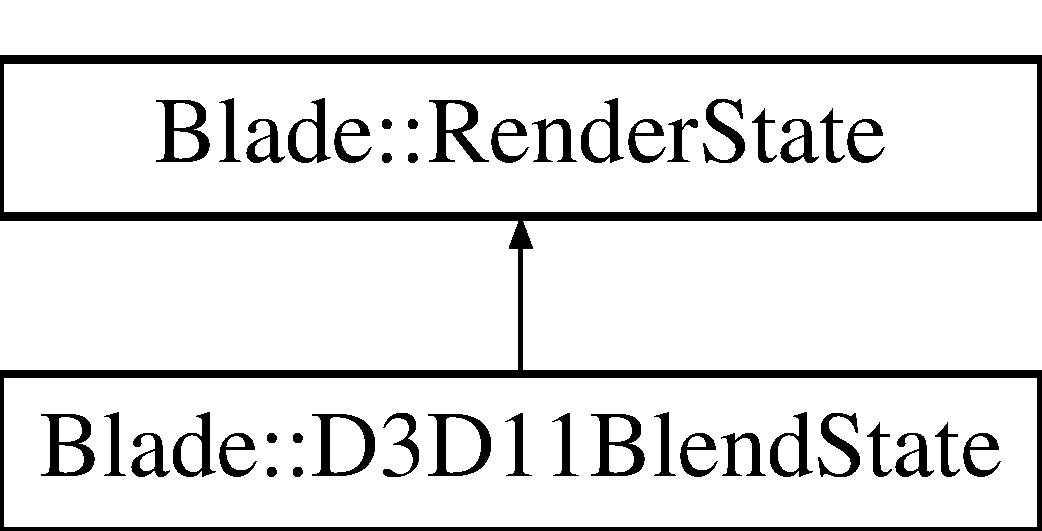
\includegraphics[height=2.000000cm]{class_blade_1_1_d3_d11_blend_state}
\end{center}
\end{figure}
\subsection*{Public Member Functions}
\begin{DoxyCompactItemize}
\item 
\mbox{\Hypertarget{class_blade_1_1_d3_d11_blend_state_a26513402cbc6899842e94c38613891af}\label{class_blade_1_1_d3_d11_blend_state_a26513402cbc6899842e94c38613891af}} 
{\bfseries D3\+D11\+Blend\+State} (Render\+State\+Type render\+\_\+state\+\_\+type)
\item 
\mbox{\Hypertarget{class_blade_1_1_d3_d11_blend_state_aea6b470c8d2c45d8dde3da2260de66f9}\label{class_blade_1_1_d3_d11_blend_state_aea6b470c8d2c45d8dde3da2260de66f9}} 
void {\bfseries Set} () const noexcept override
\end{DoxyCompactItemize}


The documentation for this class was generated from the following files\+:\begin{DoxyCompactItemize}
\item 
include/d3d/D3\+D11\+\_\+blend\+\_\+state.\+h\item 
src/d3d/D3\+D11\+\_\+blend\+\_\+state.\+cpp\end{DoxyCompactItemize}

\hypertarget{class_blade_1_1_d3_d11_context}{}\section{Blade\+:\+:D3\+D11\+Context Class Reference}
\label{class_blade_1_1_d3_d11_context}\index{Blade\+::\+D3\+D11\+Context@{Blade\+::\+D3\+D11\+Context}}
Inheritance diagram for Blade\+:\+:D3\+D11\+Context\+:\begin{figure}[H]
\begin{center}
\leavevmode
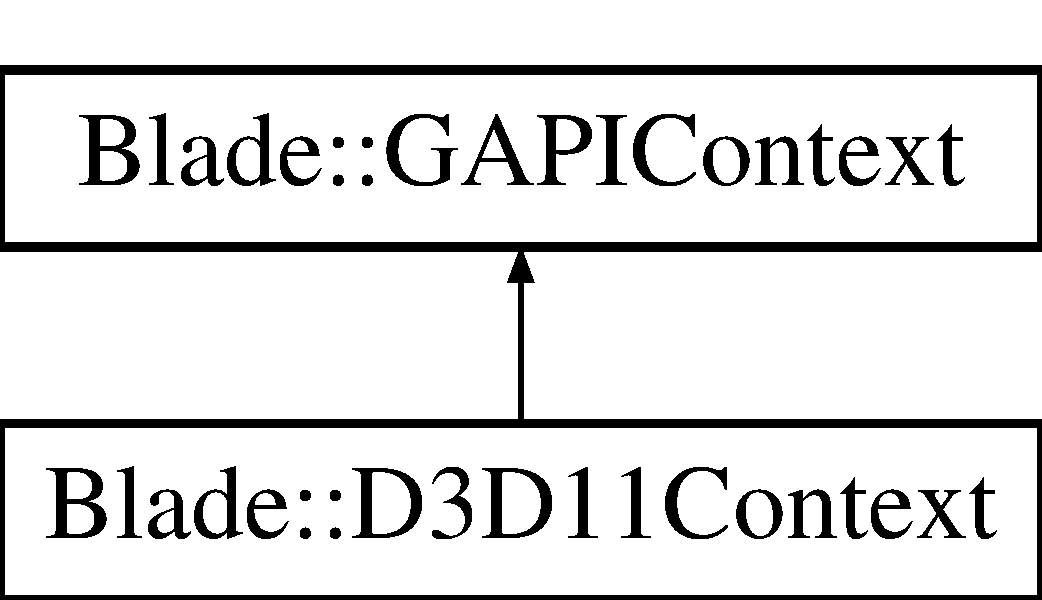
\includegraphics[height=2.000000cm]{class_blade_1_1_d3_d11_context}
\end{center}
\end{figure}
\subsection*{Public Member Functions}
\begin{DoxyCompactItemize}
\item 
\mbox{\Hypertarget{class_blade_1_1_d3_d11_context_a1a2d5dfee039abbd1676c0cb37e52c57}\label{class_blade_1_1_d3_d11_context_a1a2d5dfee039abbd1676c0cb37e52c57}} 
bool {\bfseries Create} (L\+U\+ID $\ast$luid) override
\item 
\mbox{\Hypertarget{class_blade_1_1_d3_d11_context_ac1e4c978a9e3de3d7b62977247fc1af5}\label{class_blade_1_1_d3_d11_context_ac1e4c978a9e3de3d7b62977247fc1af5}} 
I\+D3\+D11\+Device $\ast$ {\bfseries Get\+Device} () const
\item 
\mbox{\Hypertarget{class_blade_1_1_d3_d11_context_a6524137ac9799d23ad57ec3043d14fad}\label{class_blade_1_1_d3_d11_context_a6524137ac9799d23ad57ec3043d14fad}} 
I\+D3\+D11\+Device\+Context $\ast$ {\bfseries Get\+Device\+Context} () const
\item 
\mbox{\Hypertarget{class_blade_1_1_d3_d11_context_a36f3e92cfea284ca7c4005c4e72877b6}\label{class_blade_1_1_d3_d11_context_a36f3e92cfea284ca7c4005c4e72877b6}} 
I\+D3\+D11\+Debug $\ast$ {\bfseries Get\+Debug\+Interface} () const noexcept
\item 
\mbox{\Hypertarget{class_blade_1_1_d3_d11_context_ac36a54ee583e2fa174d828eaca2d71b9}\label{class_blade_1_1_d3_d11_context_ac36a54ee583e2fa174d828eaca2d71b9}} 
I\+D3\+D11\+Texture2D $\ast$ {\bfseries Get\+Back\+Buffer} () const noexcept
\item 
\mbox{\Hypertarget{class_blade_1_1_d3_d11_context_aa90193c67be01cfe7e07f5f97d7cd82e}\label{class_blade_1_1_d3_d11_context_aa90193c67be01cfe7e07f5f97d7cd82e}} 
I\+D3\+D11\+Texture2D $\ast$$\ast$ {\bfseries Get\+Address\+Of\+Back\+Buffer} () noexcept
\item 
\mbox{\Hypertarget{class_blade_1_1_d3_d11_context_a558c990e5708fff4d897fabc14e20ef6}\label{class_blade_1_1_d3_d11_context_a558c990e5708fff4d897fabc14e20ef6}} 
I\+D3\+D11\+Render\+Target\+View $\ast$ {\bfseries Get\+Default\+Render\+Target\+View} () const noexcept
\item 
\mbox{\Hypertarget{class_blade_1_1_d3_d11_context_a59a77d77ae22a58ace6629f3b5bd320a}\label{class_blade_1_1_d3_d11_context_a59a77d77ae22a58ace6629f3b5bd320a}} 
I\+D3\+D11\+Depth\+Stencil\+View $\ast$ {\bfseries Get\+Default\+Depth\+Stencil\+View} () const noexcept
\item 
\mbox{\Hypertarget{class_blade_1_1_d3_d11_context_a190680d32da401cf8c15f4a355d40fb4}\label{class_blade_1_1_d3_d11_context_a190680d32da401cf8c15f4a355d40fb4}} 
I\+D3\+D11\+Render\+Target\+View $\ast$$\ast$ {\bfseries Get\+Get\+Address\+Of\+Default\+Render\+Target\+View} () noexcept
\item 
\mbox{\Hypertarget{class_blade_1_1_d3_d11_context_aeda773a70e6a0e6f09680db3c82a9d74}\label{class_blade_1_1_d3_d11_context_aeda773a70e6a0e6f09680db3c82a9d74}} 
I\+D3\+D11\+Depth\+Stencil\+View $\ast$$\ast$ {\bfseries Get\+Address\+Of\+Default\+Depth\+Stencil\+View} () noexcept
\item 
\mbox{\Hypertarget{class_blade_1_1_d3_d11_context_a7a074c5e225360e77099b29762f6d445}\label{class_blade_1_1_d3_d11_context_a7a074c5e225360e77099b29762f6d445}} 
unsigned int {\bfseries Get\+M\+S\+A\+A\+Quality} (int sample\+\_\+count) const
\end{DoxyCompactItemize}


The documentation for this class was generated from the following files\+:\begin{DoxyCompactItemize}
\item 
include/d3d/D3\+D11\+\_\+context.\+h\item 
src/d3d/D3\+D11\+\_\+context.\+cpp\end{DoxyCompactItemize}

\hypertarget{class_blade_1_1_d3_d11_depth_stencil_state}{}\section{Blade\+:\+:D3\+D11\+Depth\+Stencil\+State Class Reference}
\label{class_blade_1_1_d3_d11_depth_stencil_state}\index{Blade\+::\+D3\+D11\+Depth\+Stencil\+State@{Blade\+::\+D3\+D11\+Depth\+Stencil\+State}}
Inheritance diagram for Blade\+:\+:D3\+D11\+Depth\+Stencil\+State\+:\begin{figure}[H]
\begin{center}
\leavevmode
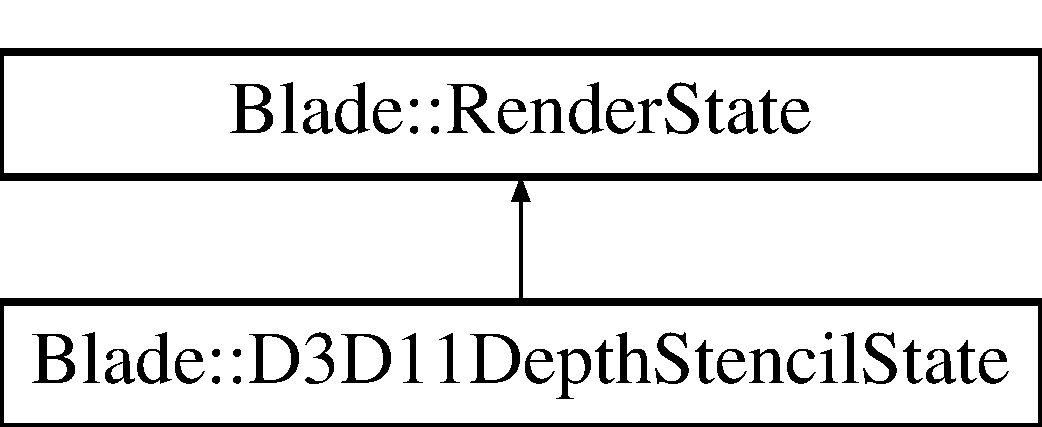
\includegraphics[height=2.000000cm]{class_blade_1_1_d3_d11_depth_stencil_state}
\end{center}
\end{figure}
\subsection*{Public Member Functions}
\begin{DoxyCompactItemize}
\item 
\mbox{\Hypertarget{class_blade_1_1_d3_d11_depth_stencil_state_a3123b3e15de065048c285af63b5b50e6}\label{class_blade_1_1_d3_d11_depth_stencil_state_a3123b3e15de065048c285af63b5b50e6}} 
{\bfseries D3\+D11\+Depth\+Stencil\+State} (Render\+State\+Type render\+State\+Type)
\item 
\mbox{\Hypertarget{class_blade_1_1_d3_d11_depth_stencil_state_a4608e15c980c00b3a13f844e106db624}\label{class_blade_1_1_d3_d11_depth_stencil_state_a4608e15c980c00b3a13f844e106db624}} 
void {\bfseries Set} () const noexcept override
\end{DoxyCompactItemize}


The documentation for this class was generated from the following files\+:\begin{DoxyCompactItemize}
\item 
include/d3d/D3\+D11\+\_\+depth\+\_\+stencil\+\_\+state.\+h\item 
src/d3d/D3\+D11\+\_\+depth\+\_\+stencil\+\_\+state.\+cpp\end{DoxyCompactItemize}

\hypertarget{class_blade_1_1_d3_d11_i_b_o}{}\section{Blade\+:\+:D3\+D11\+I\+BO Class Reference}
\label{class_blade_1_1_d3_d11_i_b_o}\index{Blade\+::\+D3\+D11\+I\+BO@{Blade\+::\+D3\+D11\+I\+BO}}
Inheritance diagram for Blade\+:\+:D3\+D11\+I\+BO\+:\begin{figure}[H]
\begin{center}
\leavevmode
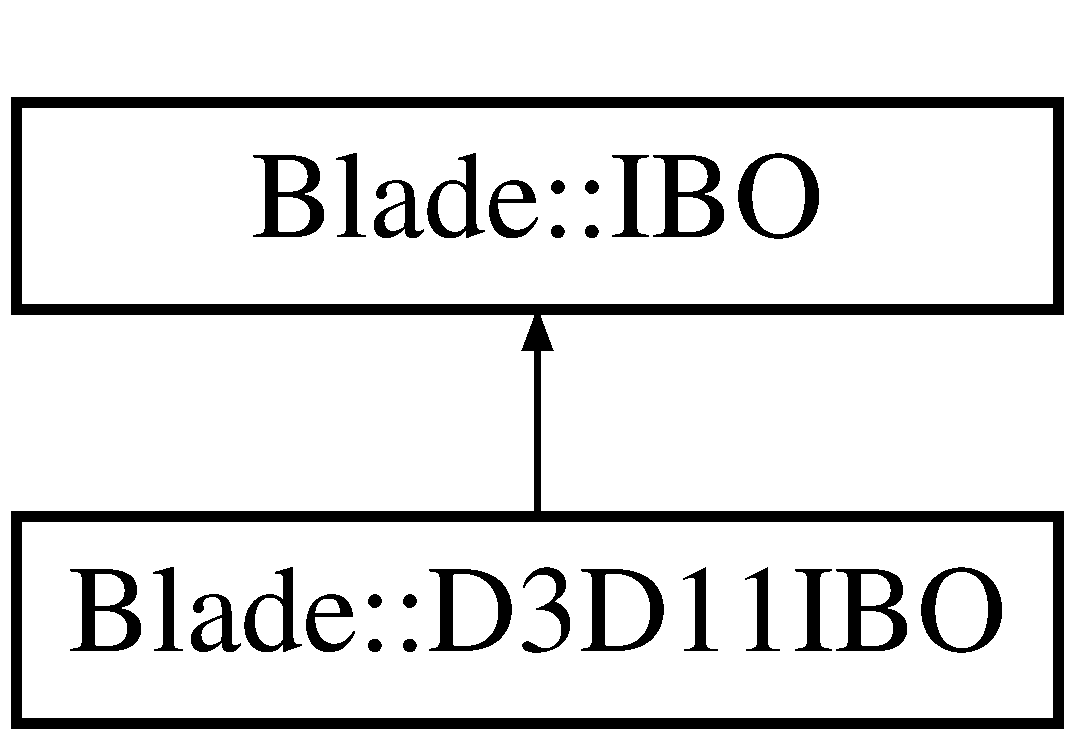
\includegraphics[height=2.000000cm]{class_blade_1_1_d3_d11_i_b_o}
\end{center}
\end{figure}
\subsection*{Public Member Functions}
\begin{DoxyCompactItemize}
\item 
\mbox{\Hypertarget{class_blade_1_1_d3_d11_i_b_o_acd953542448c159a16a7a65ddbf3ea7a}\label{class_blade_1_1_d3_d11_i_b_o_acd953542448c159a16a7a65ddbf3ea7a}} 
bool {\bfseries Create} (const std\+::vector$<$ unsigned int $>$ \&indices) noexcept override
\item 
\mbox{\Hypertarget{class_blade_1_1_d3_d11_i_b_o_ad2275cac4f7f7d50dbdd760dc7e22a63}\label{class_blade_1_1_d3_d11_i_b_o_ad2275cac4f7f7d50dbdd760dc7e22a63}} 
void {\bfseries Bind} () const noexcept override
\item 
\mbox{\Hypertarget{class_blade_1_1_d3_d11_i_b_o_adb15e836bb5627e05a3cd30e377ec5f3}\label{class_blade_1_1_d3_d11_i_b_o_adb15e836bb5627e05a3cd30e377ec5f3}} 
void {\bfseries Draw} () const noexcept override
\end{DoxyCompactItemize}


The documentation for this class was generated from the following files\+:\begin{DoxyCompactItemize}
\item 
include/d3d/D3\+D11\+\_\+\+I\+B\+O.\+h\item 
src/d3d/D3\+D11\+\_\+\+I\+B\+O.\+cpp\end{DoxyCompactItemize}

\hypertarget{class_blade_1_1_d3_d11_rasterizer_state}{}\section{Blade\+:\+:D3\+D11\+Rasterizer\+State Class Reference}
\label{class_blade_1_1_d3_d11_rasterizer_state}\index{Blade\+::\+D3\+D11\+Rasterizer\+State@{Blade\+::\+D3\+D11\+Rasterizer\+State}}
Inheritance diagram for Blade\+:\+:D3\+D11\+Rasterizer\+State\+:\begin{figure}[H]
\begin{center}
\leavevmode
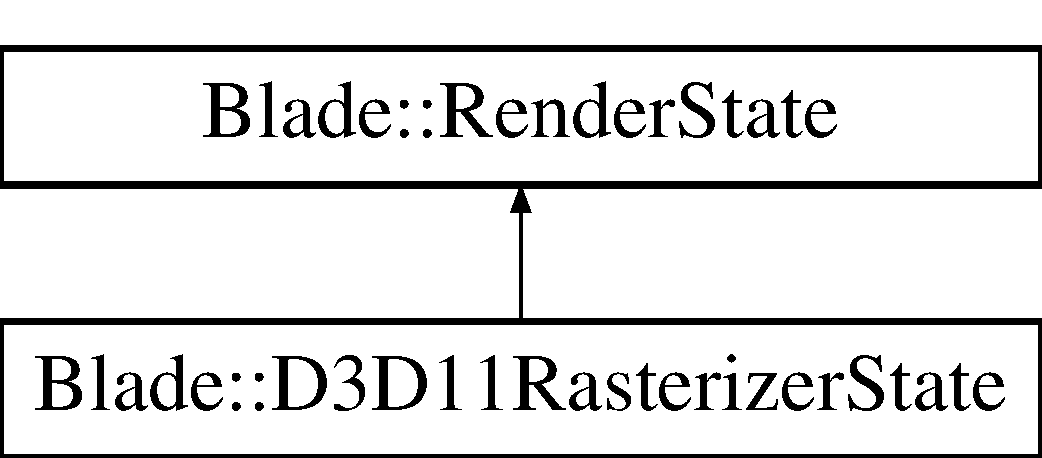
\includegraphics[height=2.000000cm]{class_blade_1_1_d3_d11_rasterizer_state}
\end{center}
\end{figure}
\subsection*{Public Member Functions}
\begin{DoxyCompactItemize}
\item 
\mbox{\Hypertarget{class_blade_1_1_d3_d11_rasterizer_state_a87077b9acce398c36a873069cf52d108}\label{class_blade_1_1_d3_d11_rasterizer_state_a87077b9acce398c36a873069cf52d108}} 
{\bfseries D3\+D11\+Rasterizer\+State} (Render\+State\+Type render\+State\+Type)
\item 
\mbox{\Hypertarget{class_blade_1_1_d3_d11_rasterizer_state_a967a3044da521170cdce48ea5e5d30d9}\label{class_blade_1_1_d3_d11_rasterizer_state_a967a3044da521170cdce48ea5e5d30d9}} 
void {\bfseries Set} () const noexcept override
\end{DoxyCompactItemize}


The documentation for this class was generated from the following files\+:\begin{DoxyCompactItemize}
\item 
include/d3d/D3\+D11\+\_\+rasterizer\+\_\+state.\+h\item 
src/d3d/D3\+D11\+\_\+rasterizer\+\_\+state.\+cpp\end{DoxyCompactItemize}

\hypertarget{class_blade_1_1_d3_d11_render_target}{}\section{Blade\+:\+:D3\+D11\+Render\+Target Class Reference}
\label{class_blade_1_1_d3_d11_render_target}\index{Blade\+::\+D3\+D11\+Render\+Target@{Blade\+::\+D3\+D11\+Render\+Target}}
Inheritance diagram for Blade\+:\+:D3\+D11\+Render\+Target\+:\begin{figure}[H]
\begin{center}
\leavevmode
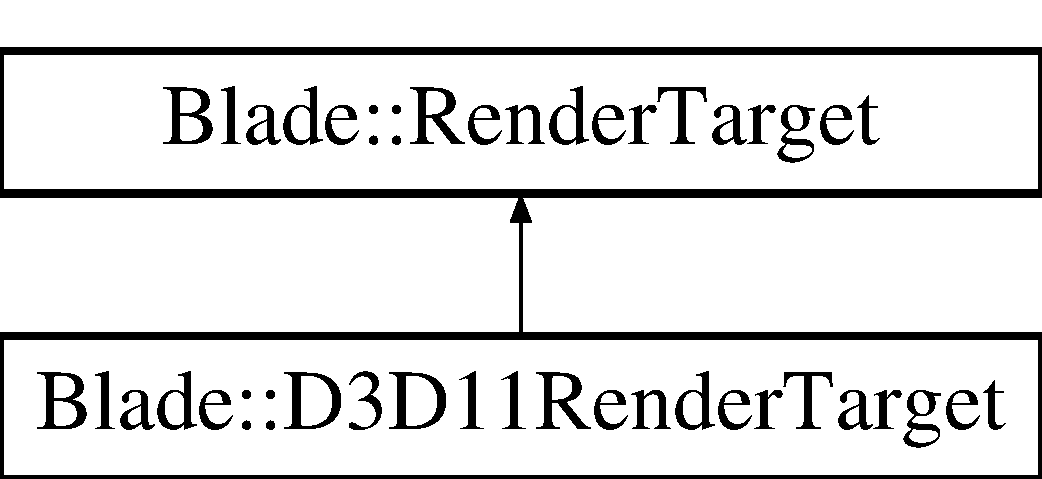
\includegraphics[height=2.000000cm]{class_blade_1_1_d3_d11_render_target}
\end{center}
\end{figure}
\subsection*{Public Member Functions}
\begin{DoxyCompactItemize}
\item 
\mbox{\Hypertarget{class_blade_1_1_d3_d11_render_target_adef14b01974b716aa68cffadacfcfd43}\label{class_blade_1_1_d3_d11_render_target_adef14b01974b716aa68cffadacfcfd43}} 
{\bfseries D3\+D11\+Render\+Target} (const Vec2i \&size, bool M\+S\+AA, int sample\+Count)
\item 
\mbox{\Hypertarget{class_blade_1_1_d3_d11_render_target_a050ec4d67f45491e1dfb92d7dfd7cc40}\label{class_blade_1_1_d3_d11_render_target_a050ec4d67f45491e1dfb92d7dfd7cc40}} 
bool {\bfseries Create} (const Vec2i \&size) override
\item 
\mbox{\Hypertarget{class_blade_1_1_d3_d11_render_target_acabe7c18fb8a6cf52a5088653c5c500d}\label{class_blade_1_1_d3_d11_render_target_acabe7c18fb8a6cf52a5088653c5c500d}} 
bool {\bfseries Bind} (Render\+Target\+Bind\+Type bind\+Type) const override
\item 
\mbox{\Hypertarget{class_blade_1_1_d3_d11_render_target_a9abf752799c1e0780dd25e4250622dfc}\label{class_blade_1_1_d3_d11_render_target_a9abf752799c1e0780dd25e4250622dfc}} 
bool {\bfseries Unbind} () const override
\item 
\mbox{\Hypertarget{class_blade_1_1_d3_d11_render_target_ae689e2c81356685e5100b6d62eef53ee}\label{class_blade_1_1_d3_d11_render_target_ae689e2c81356685e5100b6d62eef53ee}} 
void {\bfseries Clear} (float $\ast$color) const noexcept
\item 
\mbox{\Hypertarget{class_blade_1_1_d3_d11_render_target_a9430e7028c9517ba19bdb2957c649922}\label{class_blade_1_1_d3_d11_render_target_a9430e7028c9517ba19bdb2957c649922}} 
void {\bfseries Set\+Color\+Attachment} (I\+D3\+D11\+Texture2D $\ast$color\+Attachment, D\+X\+G\+I\+\_\+\+F\+O\+R\+M\+AT format) noexcept
\item 
\mbox{\Hypertarget{class_blade_1_1_d3_d11_render_target_a296069b64de6a78e2113acd49b978cb6}\label{class_blade_1_1_d3_d11_render_target_a296069b64de6a78e2113acd49b978cb6}} 
I\+D3\+D11\+Shader\+Resource\+View $\ast$ {\bfseries Get\+Color\+Attachment} () const noexcept
\item 
\mbox{\Hypertarget{class_blade_1_1_d3_d11_render_target_a3108ea56abb5804a38c0293b7034e11a}\label{class_blade_1_1_d3_d11_render_target_a3108ea56abb5804a38c0293b7034e11a}} 
I\+D3\+D11\+Shader\+Resource\+View $\ast$ {\bfseries Get\+Depth\+Attachment} () const noexcept
\end{DoxyCompactItemize}


The documentation for this class was generated from the following files\+:\begin{DoxyCompactItemize}
\item 
include/d3d/D3\+D11\+\_\+render\+\_\+target.\+h\item 
src/d3d/D3\+D11\+\_\+render\+\_\+target.\+cpp\end{DoxyCompactItemize}

\hypertarget{class_blade_1_1_d3_d11_shader}{}\section{Blade\+:\+:D3\+D11\+Shader Class Reference}
\label{class_blade_1_1_d3_d11_shader}\index{Blade\+::\+D3\+D11\+Shader@{Blade\+::\+D3\+D11\+Shader}}
Inheritance diagram for Blade\+:\+:D3\+D11\+Shader\+:\begin{figure}[H]
\begin{center}
\leavevmode
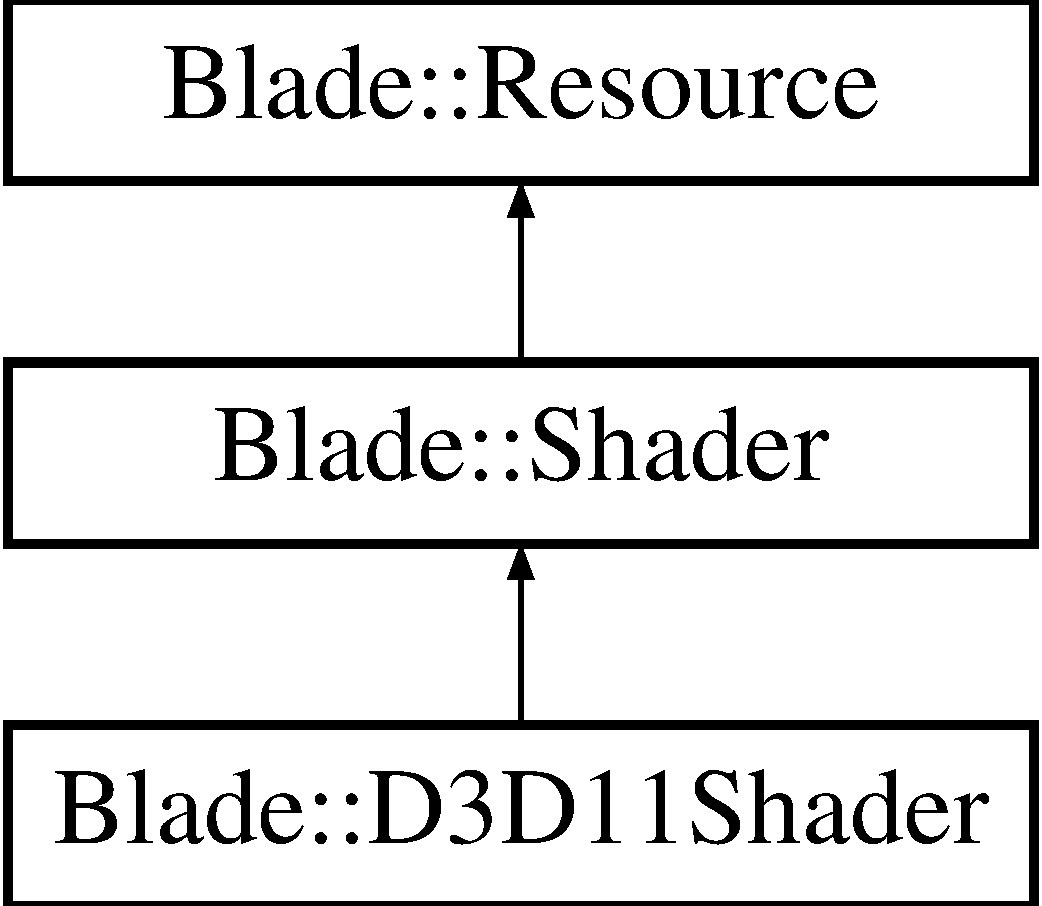
\includegraphics[height=3.000000cm]{class_blade_1_1_d3_d11_shader}
\end{center}
\end{figure}
\subsection*{Public Member Functions}
\begin{DoxyCompactItemize}
\item 
\mbox{\Hypertarget{class_blade_1_1_d3_d11_shader_a3e46be884a59d7bf6ac3142e4f8c8626}\label{class_blade_1_1_d3_d11_shader_a3e46be884a59d7bf6ac3142e4f8c8626}} 
I\+D3\+D\+Blob $\ast$ {\bfseries Get\+Blob} () const noexcept
\item 
bool \hyperlink{class_blade_1_1_d3_d11_shader_a713231594415a37d484f115478acf084}{Load} (const std\+::wstring \&file\+Name) noexcept override
\begin{DoxyCompactList}\small\item\em Load a resource form a file. \end{DoxyCompactList}\end{DoxyCompactItemize}


\subsection{Member Function Documentation}
\mbox{\Hypertarget{class_blade_1_1_d3_d11_shader_a713231594415a37d484f115478acf084}\label{class_blade_1_1_d3_d11_shader_a713231594415a37d484f115478acf084}} 
\index{Blade\+::\+D3\+D11\+Shader@{Blade\+::\+D3\+D11\+Shader}!Load@{Load}}
\index{Load@{Load}!Blade\+::\+D3\+D11\+Shader@{Blade\+::\+D3\+D11\+Shader}}
\subsubsection{\texorpdfstring{Load()}{Load()}}
{\footnotesize\ttfamily bool Blade\+::\+D3\+D11\+Shader\+::\+Load (\begin{DoxyParamCaption}\item[{const std\+::wstring \&}]{file\+\_\+name }\end{DoxyParamCaption})\hspace{0.3cm}{\ttfamily [override]}, {\ttfamily [virtual]}, {\ttfamily [noexcept]}}



Load a resource form a file. 


\begin{DoxyParams}{Parameters}
{\em file\+\_\+name} & The path of the file where the resource is stored. \\
\hline
\end{DoxyParams}
\begin{DoxyReturn}{Returns}
T\+R\+UE if the loading has been successful, false otherwise. 
\end{DoxyReturn}


Implements \hyperlink{class_blade_1_1_resource_ad89ab00a3b81df1338a8310ec92c5cff}{Blade\+::\+Resource}.



The documentation for this class was generated from the following files\+:\begin{DoxyCompactItemize}
\item 
include/d3d/D3\+D11\+\_\+shader.\+h\item 
src/d3d/D3\+D11\+\_\+shader.\+cpp\end{DoxyCompactItemize}

\hypertarget{class_blade_1_1_d3_d11_shader_program}{}\section{Blade\+:\+:D3\+D11\+Shader\+Program Class Reference}
\label{class_blade_1_1_d3_d11_shader_program}\index{Blade\+::\+D3\+D11\+Shader\+Program@{Blade\+::\+D3\+D11\+Shader\+Program}}
Inheritance diagram for Blade\+:\+:D3\+D11\+Shader\+Program\+:\begin{figure}[H]
\begin{center}
\leavevmode
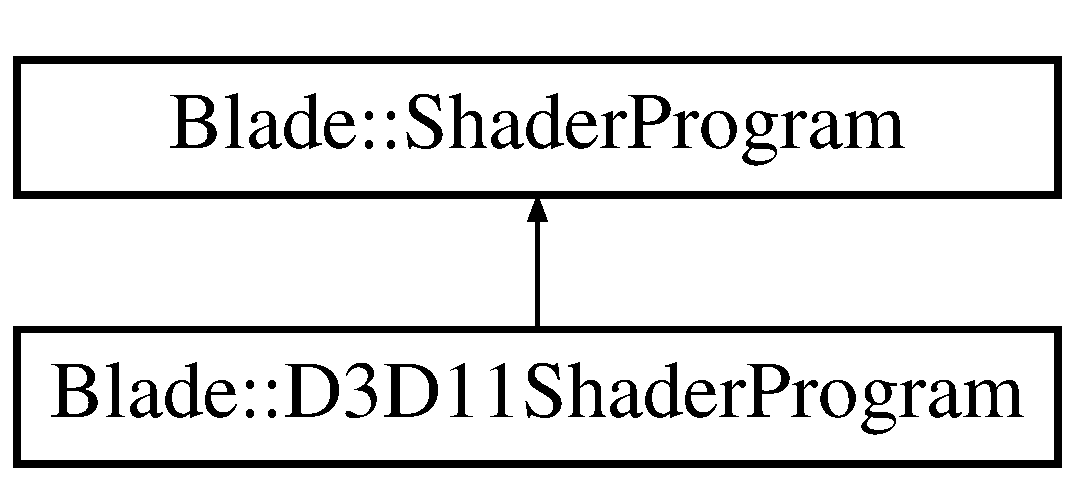
\includegraphics[height=2.000000cm]{class_blade_1_1_d3_d11_shader_program}
\end{center}
\end{figure}
\subsection*{Public Member Functions}
\begin{DoxyCompactItemize}
\item 
\mbox{\Hypertarget{class_blade_1_1_d3_d11_shader_program_a3c82d09016bc82d9b0f7b68b0b82506c}\label{class_blade_1_1_d3_d11_shader_program_a3c82d09016bc82d9b0f7b68b0b82506c}} 
bool {\bfseries Create} (const \hyperlink{struct_blade_1_1_shader_program_desc}{Shader\+Program\+Desc} \&shader\+Program\+Desc) noexcept override
\item 
\mbox{\Hypertarget{class_blade_1_1_d3_d11_shader_program_ad647764c5ca36886a85d2537d0e7e61c}\label{class_blade_1_1_d3_d11_shader_program_ad647764c5ca36886a85d2537d0e7e61c}} 
void {\bfseries Bind} () const noexcept override
\end{DoxyCompactItemize}


The documentation for this class was generated from the following files\+:\begin{DoxyCompactItemize}
\item 
include/d3d/D3\+D11\+\_\+shader\+\_\+program.\+h\item 
src/d3d/D3\+D11\+\_\+shader\+\_\+program.\+cpp\end{DoxyCompactItemize}

\hypertarget{class_blade_1_1_d3_d11_texture}{}\section{Blade\+:\+:D3\+D11\+Texture Class Reference}
\label{class_blade_1_1_d3_d11_texture}\index{Blade\+::\+D3\+D11\+Texture@{Blade\+::\+D3\+D11\+Texture}}
Inheritance diagram for Blade\+:\+:D3\+D11\+Texture\+:\begin{figure}[H]
\begin{center}
\leavevmode
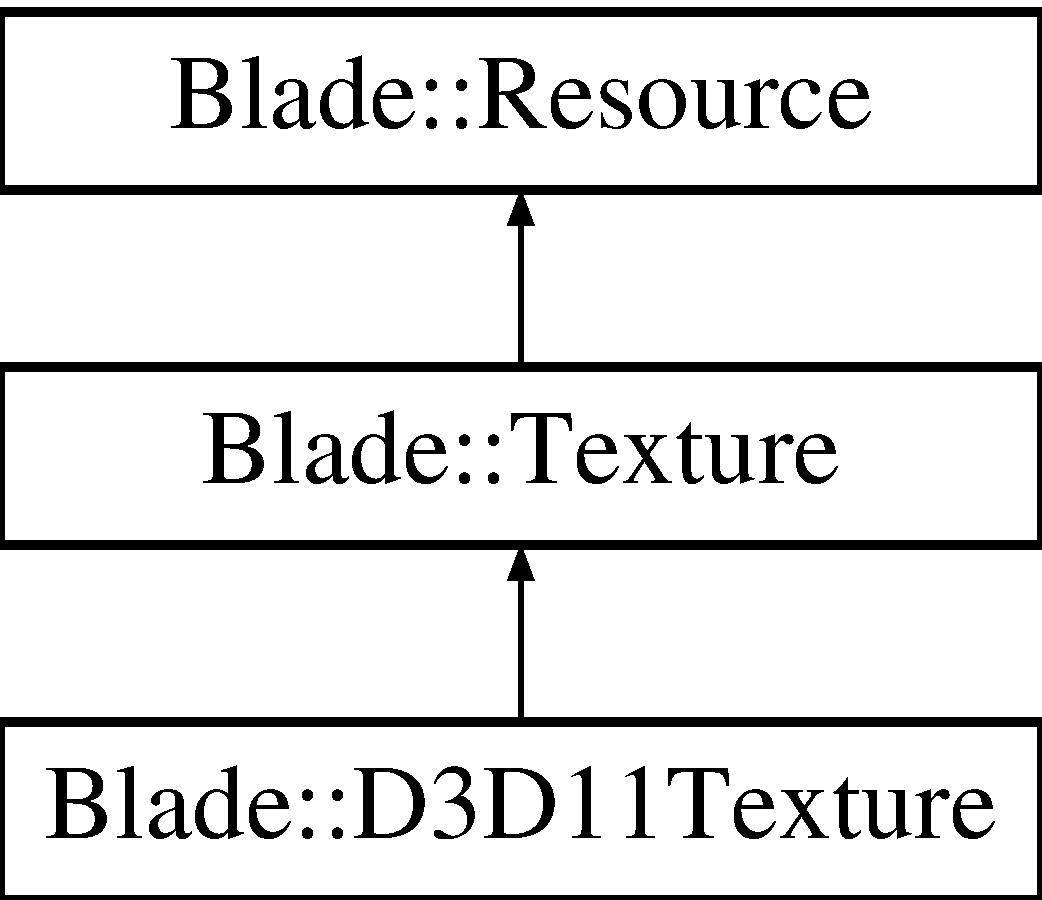
\includegraphics[height=3.000000cm]{class_blade_1_1_d3_d11_texture}
\end{center}
\end{figure}
\subsection*{Public Member Functions}
\begin{DoxyCompactItemize}
\item 
\mbox{\Hypertarget{class_blade_1_1_d3_d11_texture_ac8222f74d203b5780d6d17913d9397a7}\label{class_blade_1_1_d3_d11_texture_ac8222f74d203b5780d6d17913d9397a7}} 
{\bfseries D3\+D11\+Texture} (Texture\+Type texture\+Type)
\item 
bool \hyperlink{class_blade_1_1_d3_d11_texture_ae9f6d01709ba9db4085cf6b3d90b3ac7}{Load} (const std\+::wstring \&file\+Name) noexcept override
\begin{DoxyCompactList}\small\item\em Load a resource form a file. \end{DoxyCompactList}\item 
\mbox{\Hypertarget{class_blade_1_1_d3_d11_texture_a1e0366d9294d0435d60076b6f9291c6c}\label{class_blade_1_1_d3_d11_texture_a1e0366d9294d0435d60076b6f9291c6c}} 
void {\bfseries Bind} () const noexcept override
\end{DoxyCompactItemize}


\subsection{Member Function Documentation}
\mbox{\Hypertarget{class_blade_1_1_d3_d11_texture_ae9f6d01709ba9db4085cf6b3d90b3ac7}\label{class_blade_1_1_d3_d11_texture_ae9f6d01709ba9db4085cf6b3d90b3ac7}} 
\index{Blade\+::\+D3\+D11\+Texture@{Blade\+::\+D3\+D11\+Texture}!Load@{Load}}
\index{Load@{Load}!Blade\+::\+D3\+D11\+Texture@{Blade\+::\+D3\+D11\+Texture}}
\subsubsection{\texorpdfstring{Load()}{Load()}}
{\footnotesize\ttfamily bool Blade\+::\+D3\+D11\+Texture\+::\+Load (\begin{DoxyParamCaption}\item[{const std\+::wstring \&}]{file\+\_\+name }\end{DoxyParamCaption})\hspace{0.3cm}{\ttfamily [override]}, {\ttfamily [virtual]}, {\ttfamily [noexcept]}}



Load a resource form a file. 


\begin{DoxyParams}{Parameters}
{\em file\+\_\+name} & The path of the file where the resource is stored. \\
\hline
\end{DoxyParams}
\begin{DoxyReturn}{Returns}
T\+R\+UE if the loading has been successful, false otherwise. 
\end{DoxyReturn}


Implements \hyperlink{class_blade_1_1_resource_ad89ab00a3b81df1338a8310ec92c5cff}{Blade\+::\+Resource}.



The documentation for this class was generated from the following files\+:\begin{DoxyCompactItemize}
\item 
include/d3d/D3\+D11\+\_\+texture.\+h\item 
src/d3d/D3\+D11\+\_\+texture.\+cpp\end{DoxyCompactItemize}

\hypertarget{class_blade_1_1_d3_d11_v_b_o}{}\section{Blade\+:\+:D3\+D11\+V\+BO Class Reference}
\label{class_blade_1_1_d3_d11_v_b_o}\index{Blade\+::\+D3\+D11\+V\+BO@{Blade\+::\+D3\+D11\+V\+BO}}
Inheritance diagram for Blade\+:\+:D3\+D11\+V\+BO\+:\begin{figure}[H]
\begin{center}
\leavevmode
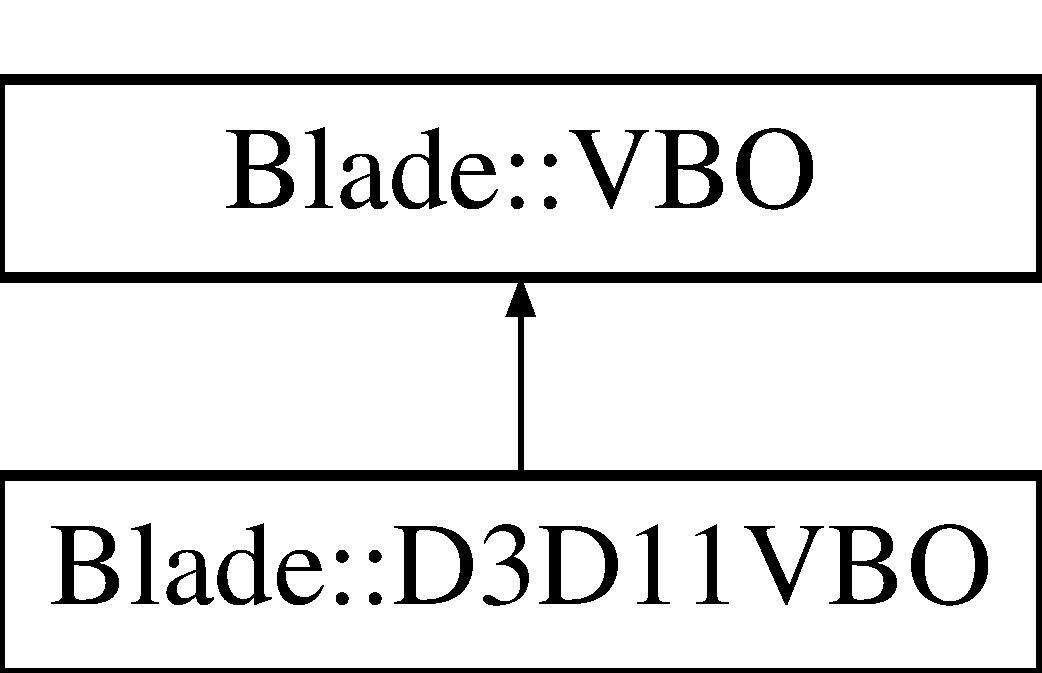
\includegraphics[height=2.000000cm]{class_blade_1_1_d3_d11_v_b_o}
\end{center}
\end{figure}
\subsection*{Public Member Functions}
\begin{DoxyCompactItemize}
\item 
\mbox{\Hypertarget{class_blade_1_1_d3_d11_v_b_o_aa30ee7b65016369210ddf1d41d2f1b67}\label{class_blade_1_1_d3_d11_v_b_o_aa30ee7b65016369210ddf1d41d2f1b67}} 
bool {\bfseries Create} (const std\+::vector$<$ \hyperlink{struct_blade_1_1_vertex}{Vertex} $>$ \&vertices, Primitive\+Topology primitive\+Topology) noexcept override
\item 
\mbox{\Hypertarget{class_blade_1_1_d3_d11_v_b_o_a0be54095e27991cfaa49344de362ec5c}\label{class_blade_1_1_d3_d11_v_b_o_a0be54095e27991cfaa49344de362ec5c}} 
void {\bfseries Bind} () const noexcept override
\item 
\mbox{\Hypertarget{class_blade_1_1_d3_d11_v_b_o_a76fd571af99bb036c429bbb310a9cabe}\label{class_blade_1_1_d3_d11_v_b_o_a76fd571af99bb036c429bbb310a9cabe}} 
void {\bfseries Draw} () const noexcept override
\end{DoxyCompactItemize}


The documentation for this class was generated from the following files\+:\begin{DoxyCompactItemize}
\item 
include/d3d/D3\+D11\+\_\+\+V\+B\+O.\+h\item 
src/d3d/D3\+D11\+\_\+\+V\+B\+O.\+cpp\end{DoxyCompactItemize}

\hypertarget{class_blade_1_1_d3_d11_viewport}{}\section{Blade\+:\+:D3\+D11\+Viewport Class Reference}
\label{class_blade_1_1_d3_d11_viewport}\index{Blade\+::\+D3\+D11\+Viewport@{Blade\+::\+D3\+D11\+Viewport}}


D3\+D11 implementation of the \hyperlink{class_blade_1_1_abstract_viewport}{Abstract\+Viewport}.  




{\ttfamily \#include $<$D3\+D11\+\_\+viewport.\+h$>$}

Inheritance diagram for Blade\+:\+:D3\+D11\+Viewport\+:\begin{figure}[H]
\begin{center}
\leavevmode
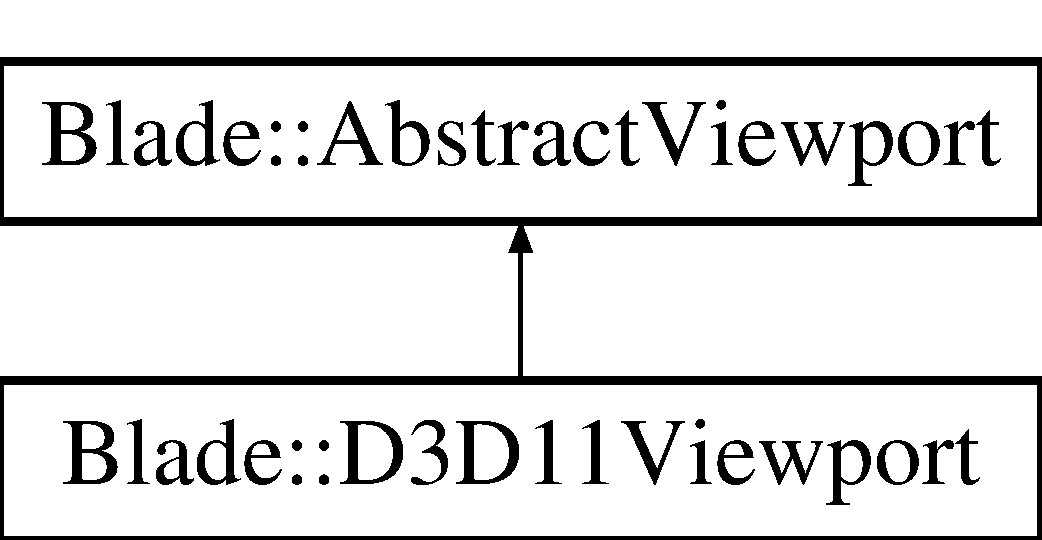
\includegraphics[height=2.000000cm]{class_blade_1_1_d3_d11_viewport}
\end{center}
\end{figure}
\subsection*{Public Member Functions}
\begin{DoxyCompactItemize}
\item 
\mbox{\Hypertarget{class_blade_1_1_d3_d11_viewport_aebaa19dcd0879142cd4626b8d326d945}\label{class_blade_1_1_d3_d11_viewport_aebaa19dcd0879142cd4626b8d326d945}} 
\hyperlink{class_blade_1_1_d3_d11_viewport_aebaa19dcd0879142cd4626b8d326d945}{D3\+D11\+Viewport} ()=default
\begin{DoxyCompactList}\small\item\em \hyperlink{class_blade_1_1_d3_d11_viewport}{D3\+D11\+Viewport} default constructor. \end{DoxyCompactList}\item 
\hyperlink{class_blade_1_1_d3_d11_viewport_aa834b9cb4de17876845f04a39bf79cd1}{D3\+D11\+Viewport} (const \hyperlink{namespace_blade_ac765e9c5c8205009994e4243d9d6f81c}{Recti} \&rect, float min\+Depth, float max\+Depth)
\begin{DoxyCompactList}\small\item\em \hyperlink{class_blade_1_1_d3_d11_viewport}{D3\+D11\+Viewport} constructor. \end{DoxyCompactList}\item 
\mbox{\Hypertarget{class_blade_1_1_d3_d11_viewport_a4c87d9aaae3d96a377344ee9c40e6ceb}\label{class_blade_1_1_d3_d11_viewport_a4c87d9aaae3d96a377344ee9c40e6ceb}} 
void \hyperlink{class_blade_1_1_d3_d11_viewport_a4c87d9aaae3d96a377344ee9c40e6ceb}{Set} () const noexcept override
\begin{DoxyCompactList}\small\item\em Sets the Viewport to the Rasterizer. \end{DoxyCompactList}\end{DoxyCompactItemize}


\subsection{Detailed Description}
D3\+D11 implementation of the \hyperlink{class_blade_1_1_abstract_viewport}{Abstract\+Viewport}. 

\subsection{Constructor \& Destructor Documentation}
\mbox{\Hypertarget{class_blade_1_1_d3_d11_viewport_aa834b9cb4de17876845f04a39bf79cd1}\label{class_blade_1_1_d3_d11_viewport_aa834b9cb4de17876845f04a39bf79cd1}} 
\index{Blade\+::\+D3\+D11\+Viewport@{Blade\+::\+D3\+D11\+Viewport}!D3\+D11\+Viewport@{D3\+D11\+Viewport}}
\index{D3\+D11\+Viewport@{D3\+D11\+Viewport}!Blade\+::\+D3\+D11\+Viewport@{Blade\+::\+D3\+D11\+Viewport}}
\subsubsection{\texorpdfstring{D3\+D11\+Viewport()}{D3D11Viewport()}}
{\footnotesize\ttfamily Blade\+::\+D3\+D11\+Viewport\+::\+D3\+D11\+Viewport (\begin{DoxyParamCaption}\item[{const \hyperlink{namespace_blade_ac765e9c5c8205009994e4243d9d6f81c}{Recti} \&}]{rect,  }\item[{float}]{min\+Depth,  }\item[{float}]{max\+Depth }\end{DoxyParamCaption})\hspace{0.3cm}{\ttfamily [inline]}}



\hyperlink{class_blade_1_1_d3_d11_viewport}{D3\+D11\+Viewport} constructor. 


\begin{DoxyParams}{Parameters}
{\em rect} & The dimensions of the viewport. \\
\hline
{\em min\+Depth} & The minimum value of the depth buffer. \\
\hline
{\em max\+Depth} & The maximum value of the depth buffer. \\
\hline
\end{DoxyParams}


The documentation for this class was generated from the following files\+:\begin{DoxyCompactItemize}
\item 
include/d3d/D3\+D11\+\_\+viewport.\+h\item 
src/d3d/D3\+D11\+\_\+viewport.\+cpp\end{DoxyCompactItemize}

\hypertarget{class_blade_1_1_d3_d11_window}{}\section{Blade\+:\+:D3\+D11\+Window Class Reference}
\label{class_blade_1_1_d3_d11_window}\index{Blade\+::\+D3\+D11\+Window@{Blade\+::\+D3\+D11\+Window}}
Inheritance diagram for Blade\+:\+:D3\+D11\+Window\+:\begin{figure}[H]
\begin{center}
\leavevmode
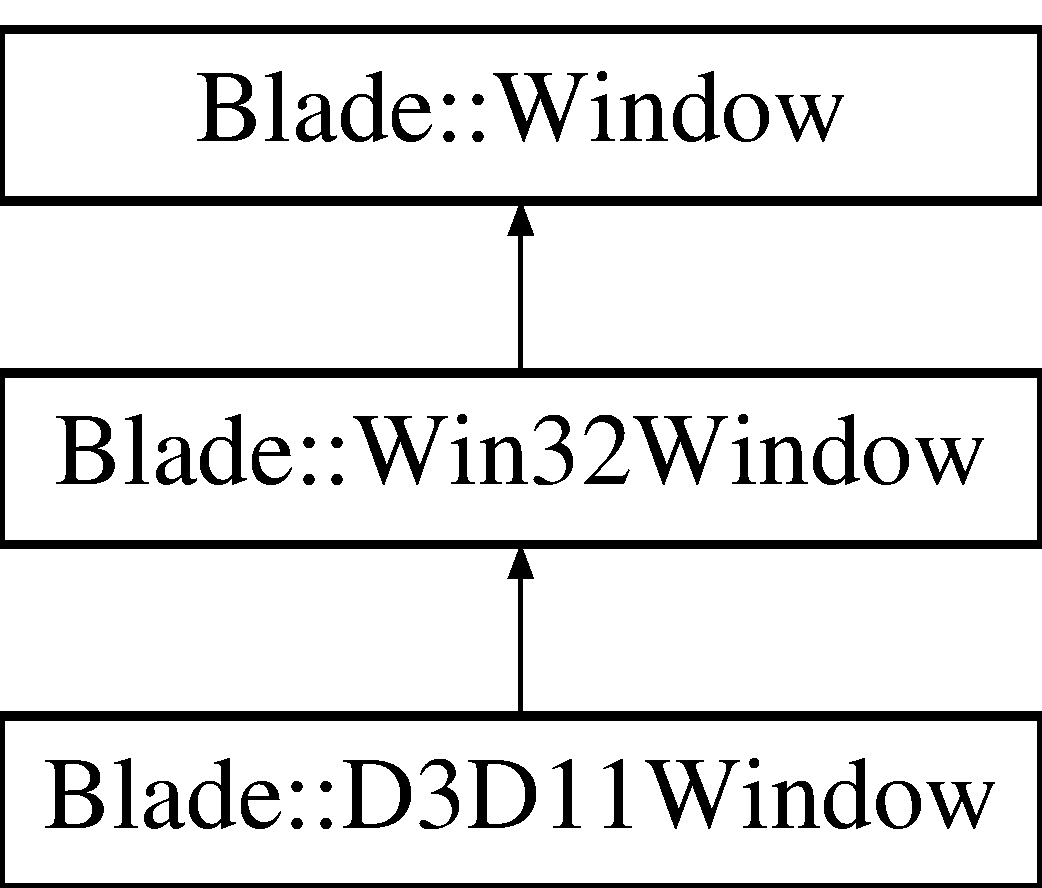
\includegraphics[height=3.000000cm]{class_blade_1_1_d3_d11_window}
\end{center}
\end{figure}
\subsection*{Public Member Functions}
\begin{DoxyCompactItemize}
\item 
\mbox{\Hypertarget{class_blade_1_1_d3_d11_window_ab14cbfe064a8a96ec88599ab90c11dab}\label{class_blade_1_1_d3_d11_window_ab14cbfe064a8a96ec88599ab90c11dab}} 
{\bfseries D3\+D11\+Window} (const std\+::wstring \&title, const Vec2i \&size, const Vec2i \&position, const unsigned int window\+Id, const bool focused, const bool minimized, const bool resizeable, const bool show\+Cursor, const bool enable\+M\+S\+AA, const int msaa\+Sample\+Count, const \hyperlink{struct_blade_1_1_window_function_callbacks}{Window\+Function\+Callbacks} \&callbacks)
\item 
\mbox{\Hypertarget{class_blade_1_1_d3_d11_window_a60102230ff52f3ef2fab1ac1c9436d75}\label{class_blade_1_1_d3_d11_window_a60102230ff52f3ef2fab1ac1c9436d75}} 
void {\bfseries Enable\+M\+S\+AA} (bool state) noexcept
\item 
\mbox{\Hypertarget{class_blade_1_1_d3_d11_window_a5605a4f289232664252d3a4762880931}\label{class_blade_1_1_d3_d11_window_a5605a4f289232664252d3a4762880931}} 
bool {\bfseries M\+S\+A\+A\+Enabled} () const noexcept
\item 
\mbox{\Hypertarget{class_blade_1_1_d3_d11_window_a1a45c76f3faeaa0e45c08a74777fb4fb}\label{class_blade_1_1_d3_d11_window_a1a45c76f3faeaa0e45c08a74777fb4fb}} 
int {\bfseries Get\+Sample\+Count} () const noexcept
\item 
\mbox{\Hypertarget{class_blade_1_1_d3_d11_window_abe617d7b324cfbf8e68f969d0a7787a6}\label{class_blade_1_1_d3_d11_window_abe617d7b324cfbf8e68f969d0a7787a6}} 
unsigned int {\bfseries Get\+M\+S\+A\+A\+Quality} () const noexcept
\item 
\mbox{\Hypertarget{class_blade_1_1_d3_d11_window_a46ab0b6ff2075dc16c84e23eb37e78fc}\label{class_blade_1_1_d3_d11_window_a46ab0b6ff2075dc16c84e23eb37e78fc}} 
void {\bfseries Swap\+Buffers} (unsigned sync\+Interval) const noexcept override
\end{DoxyCompactItemize}


The documentation for this class was generated from the following files\+:\begin{DoxyCompactItemize}
\item 
include/d3d/D3\+D11\+\_\+window.\+h\item 
src/d3d/D3\+D11\+\_\+window.\+cpp\end{DoxyCompactItemize}

\hypertarget{struct_blade_1_1_math_utils_1_1_derivative}{}\section{Blade\+:\+:Math\+Utils\+:\+:Derivative Struct Reference}
\label{struct_blade_1_1_math_utils_1_1_derivative}\index{Blade\+::\+Math\+Utils\+::\+Derivative@{Blade\+::\+Math\+Utils\+::\+Derivative}}
\subsection*{Public Attributes}
\begin{DoxyCompactItemize}
\item 
\mbox{\Hypertarget{struct_blade_1_1_math_utils_1_1_derivative_a25af28311120b67886338dc29e239442}\label{struct_blade_1_1_math_utils_1_1_derivative_a25af28311120b67886338dc29e239442}} 
float {\bfseries dx} \{ 0.\+0f \}
\item 
\mbox{\Hypertarget{struct_blade_1_1_math_utils_1_1_derivative_a48838efe113d4da5ae478493af434dfb}\label{struct_blade_1_1_math_utils_1_1_derivative_a48838efe113d4da5ae478493af434dfb}} 
float {\bfseries dv} \{ 0.\+0f \}
\end{DoxyCompactItemize}


The documentation for this struct was generated from the following file\+:\begin{DoxyCompactItemize}
\item 
include/math\+\_\+utils.\+h\end{DoxyCompactItemize}

\hypertarget{class_blade_1_1_directional_light}{}\section{Blade\+:\+:Directional\+Light Class Reference}
\label{class_blade_1_1_directional_light}\index{Blade\+::\+Directional\+Light@{Blade\+::\+Directional\+Light}}
Inheritance diagram for Blade\+:\+:Directional\+Light\+:\begin{figure}[H]
\begin{center}
\leavevmode
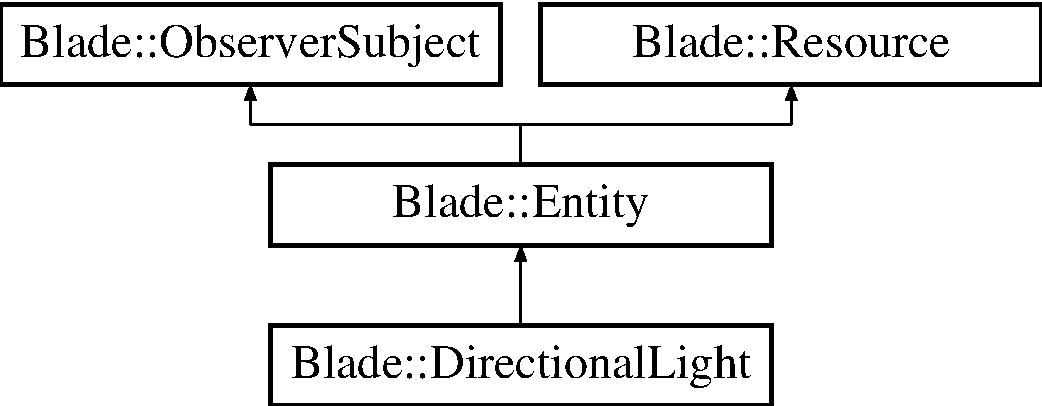
\includegraphics[height=3.000000cm]{class_blade_1_1_directional_light}
\end{center}
\end{figure}
\subsection*{Public Member Functions}
\begin{DoxyCompactItemize}
\item 
\mbox{\Hypertarget{class_blade_1_1_directional_light_a981db3910211a1e17b6099639621930f}\label{class_blade_1_1_directional_light_a981db3910211a1e17b6099639621930f}} 
{\bfseries Directional\+Light} (const std\+::string \&name, const \hyperlink{struct_blade_1_1_directional_light_desc}{Directional\+Light\+Desc} \&light\+Description)
\end{DoxyCompactItemize}


The documentation for this class was generated from the following files\+:\begin{DoxyCompactItemize}
\item 
include/directional\+\_\+light.\+h\item 
src/directional\+\_\+light.\+cpp\end{DoxyCompactItemize}

\hypertarget{class_blade_1_1_directional_light_component}{}\section{Blade\+:\+:Directional\+Light\+Component Class Reference}
\label{class_blade_1_1_directional_light_component}\index{Blade\+::\+Directional\+Light\+Component@{Blade\+::\+Directional\+Light\+Component}}
Inheritance diagram for Blade\+:\+:Directional\+Light\+Component\+:\begin{figure}[H]
\begin{center}
\leavevmode
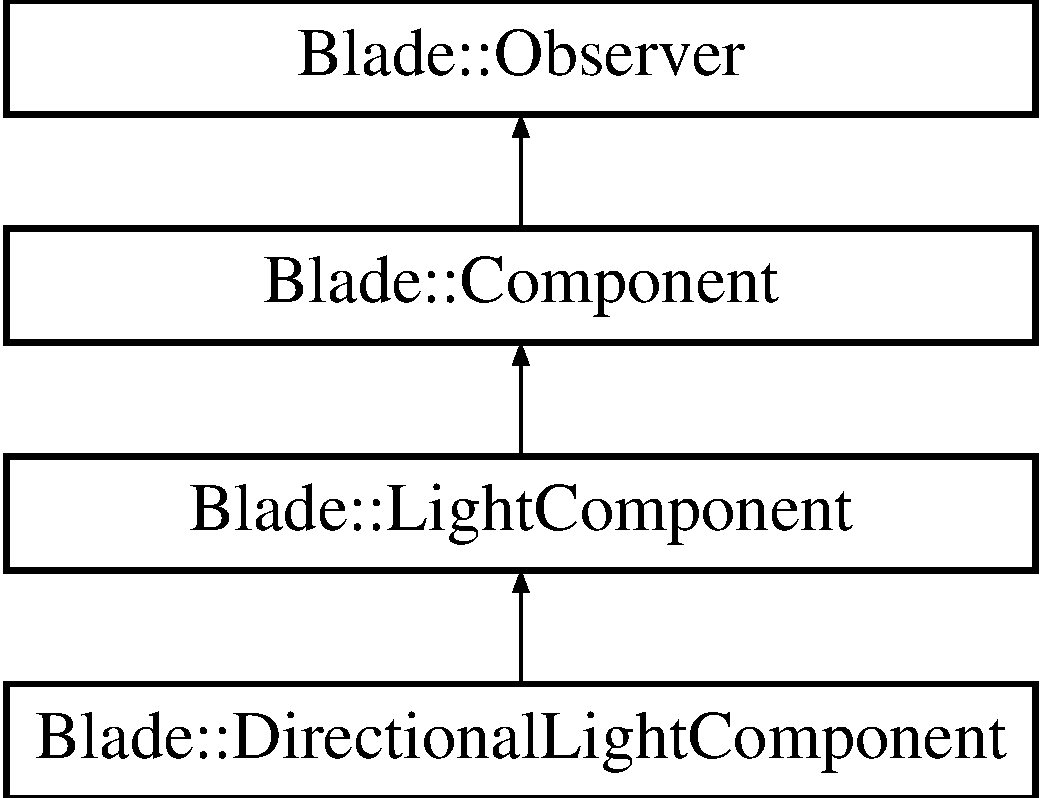
\includegraphics[height=4.000000cm]{class_blade_1_1_directional_light_component}
\end{center}
\end{figure}
\subsection*{Public Member Functions}
\begin{DoxyCompactItemize}
\item 
\mbox{\Hypertarget{class_blade_1_1_directional_light_component_a64adfd15c33a6672e7a61502bd73c9e6}\label{class_blade_1_1_directional_light_component_a64adfd15c33a6672e7a61502bd73c9e6}} 
{\bfseries Directional\+Light\+Component} (const \hyperlink{struct_blade_1_1_directional_light_desc}{Directional\+Light\+Desc} \&light\+Desc, \hyperlink{class_blade_1_1_entity}{Entity} $\ast$parent)
\item 
\mbox{\Hypertarget{class_blade_1_1_directional_light_component_a2d0e6f248ffd1417c96ae5bc9d61047c}\label{class_blade_1_1_directional_light_component_a2d0e6f248ffd1417c96ae5bc9d61047c}} 
const \hyperlink{struct_blade_1_1_directional_light_desc}{Directional\+Light\+Desc} \& {\bfseries Get\+Light\+Description} () const noexcept
\item 
\mbox{\Hypertarget{class_blade_1_1_directional_light_component_a8c2cb61aad67555b4721e2756b9e1704}\label{class_blade_1_1_directional_light_component_a8c2cb61aad67555b4721e2756b9e1704}} 
\hyperlink{struct_blade_1_1_directional_light_desc}{Directional\+Light\+Desc} $\ast$ {\bfseries Get\+Light\+Description\+Ptr} () noexcept
\end{DoxyCompactItemize}


The documentation for this class was generated from the following files\+:\begin{DoxyCompactItemize}
\item 
include/directional\+\_\+light\+\_\+component.\+h\item 
src/directional\+\_\+light\+\_\+component.\+cpp\end{DoxyCompactItemize}

\hypertarget{struct_blade_1_1_directional_light_desc}{}\section{Blade\+:\+:Directional\+Light\+Desc Struct Reference}
\label{struct_blade_1_1_directional_light_desc}\index{Blade\+::\+Directional\+Light\+Desc@{Blade\+::\+Directional\+Light\+Desc}}


A struct describing a directional light.  




{\ttfamily \#include $<$light\+\_\+component.\+h$>$}

\subsection*{Public Attributes}
\begin{DoxyCompactItemize}
\item 
\mbox{\Hypertarget{struct_blade_1_1_directional_light_desc_aed73dd21f9745383cf7fa867db98d82d}\label{struct_blade_1_1_directional_light_desc_aed73dd21f9745383cf7fa867db98d82d}} 
Vec4f {\bfseries ambient\+Intensity}
\item 
\mbox{\Hypertarget{struct_blade_1_1_directional_light_desc_a9823c4ff7f1ce4c271fbf19991c14ade}\label{struct_blade_1_1_directional_light_desc_a9823c4ff7f1ce4c271fbf19991c14ade}} 
Vec4f {\bfseries diffuse\+Intensity}
\item 
\mbox{\Hypertarget{struct_blade_1_1_directional_light_desc_aa55d775b6be27db8f7dace2cf90340ae}\label{struct_blade_1_1_directional_light_desc_aa55d775b6be27db8f7dace2cf90340ae}} 
Vec4f {\bfseries specular\+Intensity}
\item 
\mbox{\Hypertarget{struct_blade_1_1_directional_light_desc_aad27236dbfbb06db7d36c15166942094}\label{struct_blade_1_1_directional_light_desc_aad27236dbfbb06db7d36c15166942094}} 
Vec3f {\bfseries direction}
\item 
\mbox{\Hypertarget{struct_blade_1_1_directional_light_desc_aa5d519fa90e4f0db404bb2dc790ad46e}\label{struct_blade_1_1_directional_light_desc_aa5d519fa90e4f0db404bb2dc790ad46e}} 
float {\bfseries pad}
\end{DoxyCompactItemize}


\subsection{Detailed Description}
A struct describing a directional light. 

This struct is also used to represent a directional light in shaders. 

The documentation for this struct was generated from the following file\+:\begin{DoxyCompactItemize}
\item 
include/light\+\_\+component.\+h\end{DoxyCompactItemize}

\hypertarget{class_blade_1_1_emitter_component}{}\section{Blade\+:\+:Emitter\+Component Class Reference}
\label{class_blade_1_1_emitter_component}\index{Blade\+::\+Emitter\+Component@{Blade\+::\+Emitter\+Component}}
Inheritance diagram for Blade\+:\+:Emitter\+Component\+:\begin{figure}[H]
\begin{center}
\leavevmode
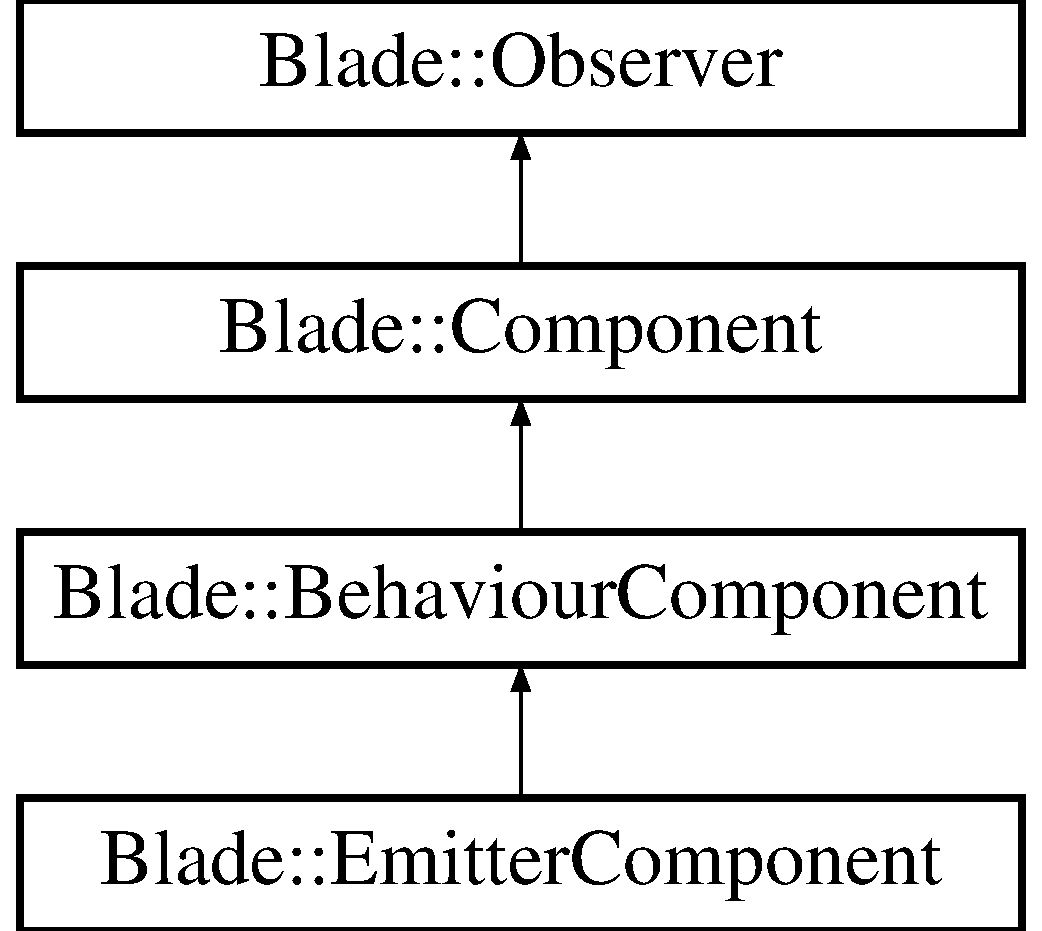
\includegraphics[height=4.000000cm]{class_blade_1_1_emitter_component}
\end{center}
\end{figure}
\subsection*{Public Member Functions}
\begin{DoxyCompactItemize}
\item 
\mbox{\Hypertarget{class_blade_1_1_emitter_component_a55cce6b7da93eaa1457bba292999a201}\label{class_blade_1_1_emitter_component_a55cce6b7da93eaa1457bba292999a201}} 
{\bfseries Emitter\+Component} (\hyperlink{class_blade_1_1_entity}{Entity} $\ast$parent)
\item 
\mbox{\Hypertarget{class_blade_1_1_emitter_component_a428197b942167146b95bc3d0faba0137}\label{class_blade_1_1_emitter_component_a428197b942167146b95bc3d0faba0137}} 
{\bfseries Emitter\+Component} (\hyperlink{class_blade_1_1_entity}{Entity} $\ast$entity, \hyperlink{struct_blade_1_1_emitter_descriptor}{Emitter\+Descriptor} descriptor)
\item 
\mbox{\Hypertarget{class_blade_1_1_emitter_component_a22e68608c870ea65bc40340bb34fd0e2}\label{class_blade_1_1_emitter_component_a22e68608c870ea65bc40340bb34fd0e2}} 
{\bfseries Emitter\+Component} (const \hyperlink{class_blade_1_1_emitter_component}{Emitter\+Component} \&other)=default
\item 
\mbox{\Hypertarget{class_blade_1_1_emitter_component_a1ab39fdf3f2931a81d16adc6d0238aa6}\label{class_blade_1_1_emitter_component_a1ab39fdf3f2931a81d16adc6d0238aa6}} 
\hyperlink{class_blade_1_1_emitter_component}{Emitter\+Component} \& {\bfseries operator=} (const \hyperlink{class_blade_1_1_emitter_component}{Emitter\+Component} \&other)=default
\item 
\mbox{\Hypertarget{class_blade_1_1_emitter_component_aa3666e4962a9b7cf05fab173524eaac8}\label{class_blade_1_1_emitter_component_aa3666e4962a9b7cf05fab173524eaac8}} 
const std\+::vector$<$ \hyperlink{struct_blade_1_1_particle}{Particle} $>$ \& {\bfseries Get\+Particles} () const noexcept
\item 
\mbox{\Hypertarget{class_blade_1_1_emitter_component_a810d5dfde0f798d23625c0e671fe7848}\label{class_blade_1_1_emitter_component_a810d5dfde0f798d23625c0e671fe7848}} 
const \hyperlink{struct_blade_1_1_emitter_descriptor}{Emitter\+Descriptor} \& {\bfseries Get\+Emitter\+Descriptor} () const noexcept
\item 
\mbox{\Hypertarget{class_blade_1_1_emitter_component_a93e1be16b0559bfbd02e537a5a51963a}\label{class_blade_1_1_emitter_component_a93e1be16b0559bfbd02e537a5a51963a}} 
void {\bfseries Set\+Descriptor} (const \hyperlink{struct_blade_1_1_emitter_descriptor}{Emitter\+Descriptor} \&descriptor) noexcept
\item 
\mbox{\Hypertarget{class_blade_1_1_emitter_component_ae4df9a88ae882bbb459ad06e140c03c7}\label{class_blade_1_1_emitter_component_ae4df9a88ae882bbb459ad06e140c03c7}} 
float {\bfseries Get\+Spawn\+Rate} () const noexcept
\item 
\mbox{\Hypertarget{class_blade_1_1_emitter_component_a6198b78c642b3c268c5fd74a799a3a78}\label{class_blade_1_1_emitter_component_a6198b78c642b3c268c5fd74a799a3a78}} 
void {\bfseries Set\+Spawn\+Rate} (const float spawn\+Rate) noexcept
\item 
\mbox{\Hypertarget{class_blade_1_1_emitter_component_a3772b5950e82280f4895322429b66cc4}\label{class_blade_1_1_emitter_component_a3772b5950e82280f4895322429b66cc4}} 
float {\bfseries Get\+Life\+Span} () const noexcept
\item 
\mbox{\Hypertarget{class_blade_1_1_emitter_component_a18ce7004fc08dd1e883847392b253a17}\label{class_blade_1_1_emitter_component_a18ce7004fc08dd1e883847392b253a17}} 
void {\bfseries Set\+Life\+Span} (const float lifespan) noexcept
\item 
\mbox{\Hypertarget{class_blade_1_1_emitter_component_a0f34fff11f8495a965ab8e63f5925535}\label{class_blade_1_1_emitter_component_a0f34fff11f8495a965ab8e63f5925535}} 
float {\bfseries Get\+Max\+Particles} () const noexcept
\item 
\mbox{\Hypertarget{class_blade_1_1_emitter_component_af372d5f7b57bed9d78a02676786ae5bc}\label{class_blade_1_1_emitter_component_af372d5f7b57bed9d78a02676786ae5bc}} 
void {\bfseries Set\+Max\+Particles} (const float max\+Particles) noexcept
\item 
\mbox{\Hypertarget{class_blade_1_1_emitter_component_a3ffa6b46a4e0ab83d5cff0c0b0b2a128}\label{class_blade_1_1_emitter_component_a3ffa6b46a4e0ab83d5cff0c0b0b2a128}} 
float {\bfseries Get\+Spawn\+Radius} () const noexcept
\item 
\mbox{\Hypertarget{class_blade_1_1_emitter_component_a7cf88ec386f9e5dacfadb9f40d98852c}\label{class_blade_1_1_emitter_component_a7cf88ec386f9e5dacfadb9f40d98852c}} 
void {\bfseries Set\+Spawn\+Radius} (const float spawn\+Radius) noexcept
\item 
\mbox{\Hypertarget{class_blade_1_1_emitter_component_aed94b4c9028483e985f214392580fa6d}\label{class_blade_1_1_emitter_component_aed94b4c9028483e985f214392580fa6d}} 
float {\bfseries Get\+Particle\+Size} () const noexcept
\item 
\mbox{\Hypertarget{class_blade_1_1_emitter_component_a6bfbacb4dc498e6887353d64162a43fd}\label{class_blade_1_1_emitter_component_a6bfbacb4dc498e6887353d64162a43fd}} 
void {\bfseries Set\+Particle\+Size} (const float particle\+Size) noexcept
\item 
\mbox{\Hypertarget{class_blade_1_1_emitter_component_ab0b5ea77ae788052705ce92f2f3d503c}\label{class_blade_1_1_emitter_component_ab0b5ea77ae788052705ce92f2f3d503c}} 
const Vec4f \& {\bfseries Get\+Start\+Color} () const noexcept
\item 
\mbox{\Hypertarget{class_blade_1_1_emitter_component_af19b7a5444da8278cdc626be085ae104}\label{class_blade_1_1_emitter_component_af19b7a5444da8278cdc626be085ae104}} 
void {\bfseries Set\+Start\+Color} (const Vec4f \&start\+Color) noexcept
\item 
\mbox{\Hypertarget{class_blade_1_1_emitter_component_af9951179ffeab5a1dbfc4275e91998b7}\label{class_blade_1_1_emitter_component_af9951179ffeab5a1dbfc4275e91998b7}} 
const Vec4f \& {\bfseries Get\+End\+Color} () const noexcept
\item 
\mbox{\Hypertarget{class_blade_1_1_emitter_component_a6ba83c77a8e201e5dda46ba4701baeda}\label{class_blade_1_1_emitter_component_a6ba83c77a8e201e5dda46ba4701baeda}} 
void {\bfseries Set\+End\+Color} (const Vec4f \&end\+Color) noexcept
\item 
\mbox{\Hypertarget{class_blade_1_1_emitter_component_a95c12cc9696a8f681a80744c7eaf07fe}\label{class_blade_1_1_emitter_component_a95c12cc9696a8f681a80744c7eaf07fe}} 
bool {\bfseries Is\+Active} () const noexcept
\item 
\mbox{\Hypertarget{class_blade_1_1_emitter_component_a469c2740608d300833249638a0cbeefe}\label{class_blade_1_1_emitter_component_a469c2740608d300833249638a0cbeefe}} 
void {\bfseries Set\+Active} (const bool active) noexcept
\item 
\mbox{\Hypertarget{class_blade_1_1_emitter_component_a9b039d1090c75e0917d9e9a9f7506442}\label{class_blade_1_1_emitter_component_a9b039d1090c75e0917d9e9a9f7506442}} 
const Vec3f \& {\bfseries Get\+Velocity} () const noexcept
\item 
\mbox{\Hypertarget{class_blade_1_1_emitter_component_aee9bdd0f76acfdee9416eb95cf32e1b2}\label{class_blade_1_1_emitter_component_aee9bdd0f76acfdee9416eb95cf32e1b2}} 
void {\bfseries Set\+Velocity} (const Vec3f \&velocity) noexcept
\item 
\mbox{\Hypertarget{class_blade_1_1_emitter_component_a173eb4eeaefadd1ee471a2f24d494369}\label{class_blade_1_1_emitter_component_a173eb4eeaefadd1ee471a2f24d494369}} 
float {\bfseries Get\+Velocity\+Range} () const noexcept
\item 
\mbox{\Hypertarget{class_blade_1_1_emitter_component_a6b621b2372cf004340ce7fee27876cef}\label{class_blade_1_1_emitter_component_a6b621b2372cf004340ce7fee27876cef}} 
void {\bfseries Set\+Velocity\+Range} (const float velocity\+Range) noexcept
\item 
\mbox{\Hypertarget{class_blade_1_1_emitter_component_a8a6ee4e0d18fa38dd1863063ba96801f}\label{class_blade_1_1_emitter_component_a8a6ee4e0d18fa38dd1863063ba96801f}} 
const Vec3f \& {\bfseries Get\+External\+Force} () const noexcept
\item 
\mbox{\Hypertarget{class_blade_1_1_emitter_component_a81753284eebd9a74f2e5792650f5c2cc}\label{class_blade_1_1_emitter_component_a81753284eebd9a74f2e5792650f5c2cc}} 
void {\bfseries Set\+External\+Force} (const Vec3f \&external\+Froce) noexcept
\item 
\mbox{\Hypertarget{class_blade_1_1_emitter_component_a82f45a55cd61b25444a9b94cf4297a09}\label{class_blade_1_1_emitter_component_a82f45a55cd61b25444a9b94cf4297a09}} 
\hyperlink{class_blade_1_1_mesh}{Mesh} $\ast$ {\bfseries Get\+Mesh} () const noexcept
\item 
\mbox{\Hypertarget{class_blade_1_1_emitter_component_ad77eb47992f071a3ca28d8763d89e566}\label{class_blade_1_1_emitter_component_ad77eb47992f071a3ca28d8763d89e566}} 
void {\bfseries Set\+Mesh} (\hyperlink{class_blade_1_1_mesh}{Mesh} $\ast$mesh) noexcept
\item 
\mbox{\Hypertarget{class_blade_1_1_emitter_component_acb800175126170cb9073fb8767b05be1}\label{class_blade_1_1_emitter_component_acb800175126170cb9073fb8767b05be1}} 
\hyperlink{class_blade_1_1_texture}{Texture} $\ast$ {\bfseries Get\+Texture} () const noexcept
\item 
\mbox{\Hypertarget{class_blade_1_1_emitter_component_ad457ad5f5355942a66d0b7a324d8b00f}\label{class_blade_1_1_emitter_component_ad457ad5f5355942a66d0b7a324d8b00f}} 
void {\bfseries Set\+Texture} (\hyperlink{class_blade_1_1_texture}{Texture} $\ast$texture) noexcept
\item 
\mbox{\Hypertarget{class_blade_1_1_emitter_component_afe6632e7c3a429f9680de72118ec1de7}\label{class_blade_1_1_emitter_component_afe6632e7c3a429f9680de72118ec1de7}} 
Render\+State\+Type {\bfseries Get\+Blend\+State\+Type} () const noexcept
\item 
\mbox{\Hypertarget{class_blade_1_1_emitter_component_a685000643bd3390b5b3bc613e0d621e3}\label{class_blade_1_1_emitter_component_a685000643bd3390b5b3bc613e0d621e3}} 
void {\bfseries Set\+Blend\+State\+Type} (Render\+State\+Type blend\+State\+Type) noexcept
\item 
void \hyperlink{class_blade_1_1_emitter_component_ac9fe8dec74fec5c575b960cc9d1411ac}{Update} (const float dt, const long time) noexcept override
\begin{DoxyCompactList}\small\item\em Updates the \hyperlink{class_blade_1_1_component}{Component} on each frame. \end{DoxyCompactList}\item 
\mbox{\Hypertarget{class_blade_1_1_emitter_component_a996bcbc1a5869b1b1bbf1e7a4124b1ed}\label{class_blade_1_1_emitter_component_a996bcbc1a5869b1b1bbf1e7a4124b1ed}} 
void \hyperlink{class_blade_1_1_emitter_component_a996bcbc1a5869b1b1bbf1e7a4124b1ed}{Setup} () noexcept override
\begin{DoxyCompactList}\small\item\em Performs setup actions after the \hyperlink{class_blade_1_1_behaviour_component}{Behaviour\+Component}\textquotesingle{}s creation. \end{DoxyCompactList}\item 
\mbox{\Hypertarget{class_blade_1_1_emitter_component_a434f1134ef21f15a6839c6e66b282fd3}\label{class_blade_1_1_emitter_component_a434f1134ef21f15a6839c6e66b282fd3}} 
void \hyperlink{class_blade_1_1_emitter_component_a434f1134ef21f15a6839c6e66b282fd3}{Teardown} () noexcept override
\begin{DoxyCompactList}\small\item\em Performs actions before the \hyperlink{class_blade_1_1_behaviour_component}{Behaviour\+Component} is destroyed. \end{DoxyCompactList}\end{DoxyCompactItemize}


\subsection{Member Function Documentation}
\mbox{\Hypertarget{class_blade_1_1_emitter_component_ac9fe8dec74fec5c575b960cc9d1411ac}\label{class_blade_1_1_emitter_component_ac9fe8dec74fec5c575b960cc9d1411ac}} 
\index{Blade\+::\+Emitter\+Component@{Blade\+::\+Emitter\+Component}!Update@{Update}}
\index{Update@{Update}!Blade\+::\+Emitter\+Component@{Blade\+::\+Emitter\+Component}}
\subsubsection{\texorpdfstring{Update()}{Update()}}
{\footnotesize\ttfamily void Blade\+::\+Emitter\+Component\+::\+Update (\begin{DoxyParamCaption}\item[{const float}]{dt,  }\item[{const long}]{time }\end{DoxyParamCaption})\hspace{0.3cm}{\ttfamily [override]}, {\ttfamily [virtual]}, {\ttfamily [noexcept]}}



Updates the \hyperlink{class_blade_1_1_component}{Component} on each frame. 


\begin{DoxyParams}{Parameters}
{\em dt} & The time elapsed from the previous frame of the \hyperlink{class_blade_1_1_application}{Application}. \\
\hline
{\em time} & The elapsed time since the start of the \hyperlink{class_blade_1_1_application}{Application}. \\
\hline
\end{DoxyParams}


Implements \hyperlink{class_blade_1_1_behaviour_component_a90ec3079534ea1f7225c676881b30c17}{Blade\+::\+Behaviour\+Component}.



The documentation for this class was generated from the following files\+:\begin{DoxyCompactItemize}
\item 
include/emitter\+\_\+component.\+h\item 
src/emitter\+\_\+component.\+cpp\end{DoxyCompactItemize}

\hypertarget{struct_blade_1_1_emitter_descriptor}{}\section{Blade\+:\+:Emitter\+Descriptor Struct Reference}
\label{struct_blade_1_1_emitter_descriptor}\index{Blade\+::\+Emitter\+Descriptor@{Blade\+::\+Emitter\+Descriptor}}
Inheritance diagram for Blade\+:\+:Emitter\+Descriptor\+:\begin{figure}[H]
\begin{center}
\leavevmode
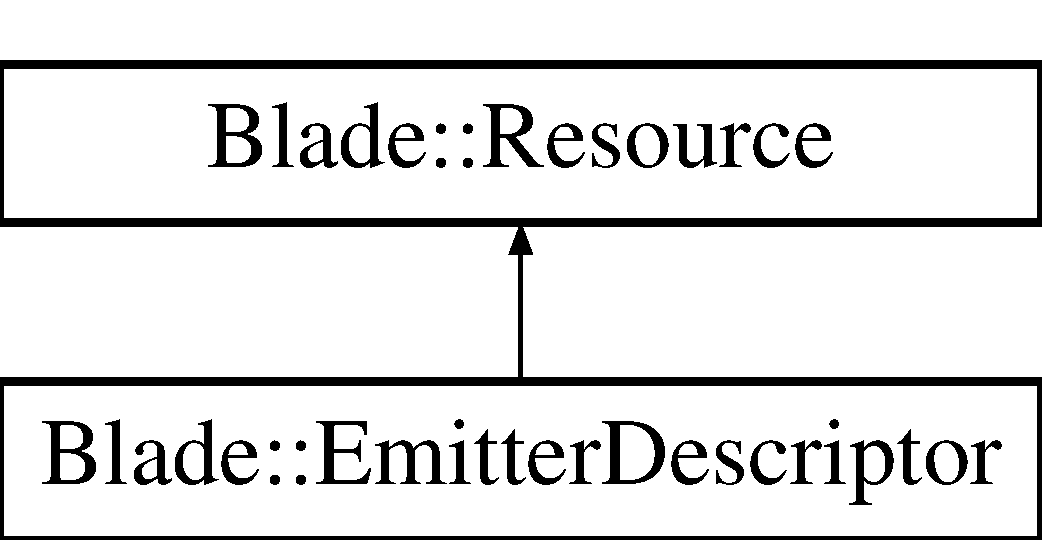
\includegraphics[height=2.000000cm]{struct_blade_1_1_emitter_descriptor}
\end{center}
\end{figure}
\subsection*{Public Member Functions}
\begin{DoxyCompactItemize}
\item 
\mbox{\Hypertarget{struct_blade_1_1_emitter_descriptor_ac3bf4ccedee573630235f498a0c47822}\label{struct_blade_1_1_emitter_descriptor_ac3bf4ccedee573630235f498a0c47822}} 
bool {\bfseries Load} (const std\+::wstring \&file\+\_\+name) noexcept override
\end{DoxyCompactItemize}
\subsection*{Public Attributes}
\begin{DoxyCompactItemize}
\item 
\mbox{\Hypertarget{struct_blade_1_1_emitter_descriptor_a27346a758b2ef3421ea4147db5a441db}\label{struct_blade_1_1_emitter_descriptor_a27346a758b2ef3421ea4147db5a441db}} 
Vec3f {\bfseries velocity}
\item 
\mbox{\Hypertarget{struct_blade_1_1_emitter_descriptor_a2dce140552513916fb01066ff837bd35}\label{struct_blade_1_1_emitter_descriptor_a2dce140552513916fb01066ff837bd35}} 
Vec3f {\bfseries external\+Force}
\item 
\mbox{\Hypertarget{struct_blade_1_1_emitter_descriptor_a16ea6f637dca0c41ebeb41f20aa79024}\label{struct_blade_1_1_emitter_descriptor_a16ea6f637dca0c41ebeb41f20aa79024}} 
float {\bfseries spawn\+Rate}
\item 
\mbox{\Hypertarget{struct_blade_1_1_emitter_descriptor_a677f1e5456b5c2ff2eea43adf1f3fbcc}\label{struct_blade_1_1_emitter_descriptor_a677f1e5456b5c2ff2eea43adf1f3fbcc}} 
float {\bfseries lifespan}
\item 
\mbox{\Hypertarget{struct_blade_1_1_emitter_descriptor_a1545f48e864c7546fd96bb217a168e37}\label{struct_blade_1_1_emitter_descriptor_a1545f48e864c7546fd96bb217a168e37}} 
float {\bfseries max\+Particles}
\item 
\mbox{\Hypertarget{struct_blade_1_1_emitter_descriptor_a17e8ad3957e0ca2e4617c08be19c1893}\label{struct_blade_1_1_emitter_descriptor_a17e8ad3957e0ca2e4617c08be19c1893}} 
float {\bfseries spawn\+Radius}
\item 
\mbox{\Hypertarget{struct_blade_1_1_emitter_descriptor_a1c18887f9ad86dd43b1ea0463ff2e2c2}\label{struct_blade_1_1_emitter_descriptor_a1c18887f9ad86dd43b1ea0463ff2e2c2}} 
float {\bfseries particle\+Size}
\item 
\mbox{\Hypertarget{struct_blade_1_1_emitter_descriptor_aedb1dd8d7c3137d33a551673d234397e}\label{struct_blade_1_1_emitter_descriptor_aedb1dd8d7c3137d33a551673d234397e}} 
Vec4f {\bfseries start\+Color}
\item 
\mbox{\Hypertarget{struct_blade_1_1_emitter_descriptor_a5396df2b57d60c46a36ec2fd788e7c28}\label{struct_blade_1_1_emitter_descriptor_a5396df2b57d60c46a36ec2fd788e7c28}} 
Vec4f {\bfseries end\+Color}
\item 
\mbox{\Hypertarget{struct_blade_1_1_emitter_descriptor_abd4901b9e39078ff756395df0a917660}\label{struct_blade_1_1_emitter_descriptor_abd4901b9e39078ff756395df0a917660}} 
\hyperlink{class_blade_1_1_texture}{Texture} $\ast$ {\bfseries texture}
\item 
\mbox{\Hypertarget{struct_blade_1_1_emitter_descriptor_a157b590550eb8587ead1968030ae432a}\label{struct_blade_1_1_emitter_descriptor_a157b590550eb8587ead1968030ae432a}} 
Render\+State\+Type {\bfseries blend\+State\+Type}
\item 
\mbox{\Hypertarget{struct_blade_1_1_emitter_descriptor_a2f0d7f9a227f3f5e6d816b14ec18d7f2}\label{struct_blade_1_1_emitter_descriptor_a2f0d7f9a227f3f5e6d816b14ec18d7f2}} 
float {\bfseries particles\+To\+Spawn} \{ 0 \}
\item 
\mbox{\Hypertarget{struct_blade_1_1_emitter_descriptor_a93476142c0c33f767d355b400ab0845c}\label{struct_blade_1_1_emitter_descriptor_a93476142c0c33f767d355b400ab0845c}} 
float {\bfseries velocity\+Range}
\item 
\mbox{\Hypertarget{struct_blade_1_1_emitter_descriptor_a84142b39476686f7f68c1cf8bb8ef6b1}\label{struct_blade_1_1_emitter_descriptor_a84142b39476686f7f68c1cf8bb8ef6b1}} 
bool {\bfseries active}
\end{DoxyCompactItemize}


The documentation for this struct was generated from the following files\+:\begin{DoxyCompactItemize}
\item 
include/emitter\+\_\+component.\+h\item 
src/emitter\+\_\+component.\+cpp\end{DoxyCompactItemize}

\hypertarget{class_blade_1_1_engine_context}{}\section{Blade\+:\+:Engine\+Context Class Reference}
\label{class_blade_1_1_engine_context}\index{Blade\+::\+Engine\+Context@{Blade\+::\+Engine\+Context}}
\subsection*{Public Member Functions}
\begin{DoxyCompactItemize}
\item 
\mbox{\Hypertarget{class_blade_1_1_engine_context_a0432518913109c1063dea7a3b60b267d}\label{class_blade_1_1_engine_context_a0432518913109c1063dea7a3b60b267d}} 
{\bfseries Engine\+Context} (const \hyperlink{class_blade_1_1_engine_context}{Engine\+Context} \&context)=delete
\item 
\mbox{\Hypertarget{class_blade_1_1_engine_context_acd3fdd09e0fb837f5ebd78aac9360748}\label{class_blade_1_1_engine_context_acd3fdd09e0fb837f5ebd78aac9360748}} 
\hyperlink{class_blade_1_1_engine_context}{Engine\+Context} \& {\bfseries operator=} (const \hyperlink{class_blade_1_1_engine_context}{Engine\+Context} \&context)=delete
\end{DoxyCompactItemize}
\subsection*{Static Public Member Functions}
\begin{DoxyCompactItemize}
\item 
\mbox{\Hypertarget{class_blade_1_1_engine_context_a33f15f91dfa8e4c84de083c27ab98d86}\label{class_blade_1_1_engine_context_a33f15f91dfa8e4c84de083c27ab98d86}} 
static bool {\bfseries Initialize} ()
\item 
\mbox{\Hypertarget{class_blade_1_1_engine_context_a4ceab253aad2d1d0263f742f454e674c}\label{class_blade_1_1_engine_context_a4ceab253aad2d1d0263f742f454e674c}} 
static \hyperlink{class_blade_1_1_thread_pool}{Thread\+Pool} \& {\bfseries Get\+Thread\+Pool} () noexcept
\item 
\mbox{\Hypertarget{class_blade_1_1_engine_context_a9de91f1e7fcf28a5f5cf331852b60d91}\label{class_blade_1_1_engine_context_a9de91f1e7fcf28a5f5cf331852b60d91}} 
static \hyperlink{class_blade_1_1_render_system}{Render\+System} \& {\bfseries Get\+Render\+System} () noexcept
\item 
\mbox{\Hypertarget{class_blade_1_1_engine_context_aaddcd3c7718c2feb60123886add4c7e4}\label{class_blade_1_1_engine_context_aaddcd3c7718c2feb60123886add4c7e4}} 
static \hyperlink{class_blade_1_1_camera_system}{Camera\+System} \& {\bfseries Get\+Camera\+System} () noexcept
\item 
\mbox{\Hypertarget{class_blade_1_1_engine_context_a6e5facbcc140f77d56256099235cfb29}\label{class_blade_1_1_engine_context_a6e5facbcc140f77d56256099235cfb29}} 
static \hyperlink{class_blade_1_1_light_system}{Light\+System} \& {\bfseries Get\+Light\+System} () noexcept
\item 
\mbox{\Hypertarget{class_blade_1_1_engine_context_a198c8461bd9afb1e50938066d694df16}\label{class_blade_1_1_engine_context_a198c8461bd9afb1e50938066d694df16}} 
static \hyperlink{class_blade_1_1_simulation_system}{Simulation\+System} \& {\bfseries Get\+Simulation\+System} () noexcept
\item 
\mbox{\Hypertarget{class_blade_1_1_engine_context_acb45de32a4850bcd083b9f16631c86a8}\label{class_blade_1_1_engine_context_acb45de32a4850bcd083b9f16631c86a8}} 
static \hyperlink{class_blade_1_1_behaviour_system}{Behaviour\+System} \& {\bfseries Get\+Behaviour\+System} () noexcept
\item 
\mbox{\Hypertarget{class_blade_1_1_engine_context_a1eeb49387ae175dacfbbc1c2bd84d68c}\label{class_blade_1_1_engine_context_a1eeb49387ae175dacfbbc1c2bd84d68c}} 
static \hyperlink{class_blade_1_1_network_manager}{Network\+Manager} \& {\bfseries Get\+Network\+Manager} () noexcept
\item 
\mbox{\Hypertarget{class_blade_1_1_engine_context_a31c0db645fa12534692516f7f5ae270f}\label{class_blade_1_1_engine_context_a31c0db645fa12534692516f7f5ae270f}} 
static \hyperlink{class_blade_1_1_render_state_manager}{Render\+State\+Manager} \& {\bfseries Get\+Render\+State\+Manager} () noexcept
\item 
\mbox{\Hypertarget{class_blade_1_1_engine_context_a8335eb461fad9d929028158c4f389ffa}\label{class_blade_1_1_engine_context_a8335eb461fad9d929028158c4f389ffa}} 
static \hyperlink{class_blade_1_1_resource_manager}{Resource\+Manager} \& {\bfseries Get\+Resource\+Manager} () noexcept
\item 
\mbox{\Hypertarget{class_blade_1_1_engine_context_a377c7a9650027e9bf635bcfa2a2cb5d5}\label{class_blade_1_1_engine_context_a377c7a9650027e9bf635bcfa2a2cb5d5}} 
static \hyperlink{class_blade_1_1_scene_manager}{Scene\+Manager} \& {\bfseries Get\+Scene\+Manager} () noexcept
\item 
\mbox{\Hypertarget{class_blade_1_1_engine_context_a0d3725af9576da43c54ec182b0bb797f}\label{class_blade_1_1_engine_context_a0d3725af9576da43c54ec182b0bb797f}} 
static \hyperlink{class_blade_1_1_shader_program_manager}{Shader\+Program\+Manager} \& {\bfseries Get\+Shader\+Program\+Manager} () noexcept
\item 
\mbox{\Hypertarget{class_blade_1_1_engine_context_aa4fcca132d847fe4c9ee9a16b7e347d3}\label{class_blade_1_1_engine_context_aa4fcca132d847fe4c9ee9a16b7e347d3}} 
static \hyperlink{class_blade_1_1_input_manager}{Input\+Manager} \& {\bfseries Get\+Input\+Manager} () noexcept
\item 
\mbox{\Hypertarget{class_blade_1_1_engine_context_aca2df73f49a3b33af733e1c04cdef040}\label{class_blade_1_1_engine_context_aca2df73f49a3b33af733e1c04cdef040}} 
static \hyperlink{class_blade_1_1_particle_system}{Particle\+System} \& {\bfseries Get\+Particle\+System} () noexcept
\item 
\mbox{\Hypertarget{class_blade_1_1_engine_context_a1cb4db31c19ed43f5050cafd57b78bde}\label{class_blade_1_1_engine_context_a1cb4db31c19ed43f5050cafd57b78bde}} 
static void {\bfseries Register\+Application} (\hyperlink{class_blade_1_1_application}{Application} $\ast$application) noexcept
\item 
\mbox{\Hypertarget{class_blade_1_1_engine_context_aa3f0da18a061c021d031951b68e461c9}\label{class_blade_1_1_engine_context_aa3f0da18a061c021d031951b68e461c9}} 
static \hyperlink{class_blade_1_1_application}{Application} \& {\bfseries Get\+Application} () noexcept
\item 
\mbox{\Hypertarget{class_blade_1_1_engine_context_a0fbfe001768f56cc80437751bd453225}\label{class_blade_1_1_engine_context_a0fbfe001768f56cc80437751bd453225}} 
static \hyperlink{class_blade_1_1_audio_manager}{Audio\+Manager} \& {\bfseries Get\+Audio\+Manager} () noexcept
\end{DoxyCompactItemize}


The documentation for this class was generated from the following files\+:\begin{DoxyCompactItemize}
\item 
include/engine\+\_\+context.\+h\item 
src/engine\+\_\+context.\+cpp\end{DoxyCompactItemize}

\hypertarget{class_blade_1_1_entity}{}\section{Blade\+:\+:Entity Class Reference}
\label{class_blade_1_1_entity}\index{Blade\+::\+Entity@{Blade\+::\+Entity}}
Inheritance diagram for Blade\+:\+:Entity\+:\begin{figure}[H]
\begin{center}
\leavevmode
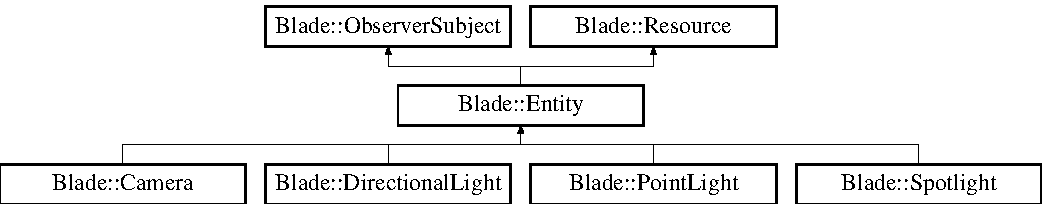
\includegraphics[height=2.727273cm]{class_blade_1_1_entity}
\end{center}
\end{figure}
\subsection*{Public Member Functions}
\begin{DoxyCompactItemize}
\item 
\mbox{\Hypertarget{class_blade_1_1_entity_a6d34bb601af516537890e7eb34324887}\label{class_blade_1_1_entity_a6d34bb601af516537890e7eb34324887}} 
{\bfseries Entity} (const std\+::string \&name)
\item 
\mbox{\Hypertarget{class_blade_1_1_entity_a78520c1c2c0e3bc3e259053d4299da92}\label{class_blade_1_1_entity_a78520c1c2c0e3bc3e259053d4299da92}} 
{\bfseries Entity} (const \hyperlink{class_blade_1_1_entity}{Entity} \&other)
\item 
\mbox{\Hypertarget{class_blade_1_1_entity_a55d9348cb6292911799415ca9a344dfc}\label{class_blade_1_1_entity_a55d9348cb6292911799415ca9a344dfc}} 
\hyperlink{class_blade_1_1_entity}{Entity} \& {\bfseries operator=} (const \hyperlink{class_blade_1_1_entity}{Entity} \&other)
\item 
\mbox{\Hypertarget{class_blade_1_1_entity_a8a71a64caa88b47b6218174a2cde1308}\label{class_blade_1_1_entity_a8a71a64caa88b47b6218174a2cde1308}} 
const std\+::string \& {\bfseries Get\+Name} () const noexcept
\item 
\mbox{\Hypertarget{class_blade_1_1_entity_a68bc45aa86d40320388cad65ad7f9e0d}\label{class_blade_1_1_entity_a68bc45aa86d40320388cad65ad7f9e0d}} 
const Vec3f \& {\bfseries Get\+Local\+Position} () const noexcept
\item 
\mbox{\Hypertarget{class_blade_1_1_entity_a3cd447ee5d8945ce3b17986ee7ed528a}\label{class_blade_1_1_entity_a3cd447ee5d8945ce3b17986ee7ed528a}} 
Vec3f {\bfseries Get\+World\+Position} () noexcept
\item 
\mbox{\Hypertarget{class_blade_1_1_entity_a451527105bd9298c9dc04f2afdedd9c5}\label{class_blade_1_1_entity_a451527105bd9298c9dc04f2afdedd9c5}} 
void {\bfseries Set\+Position} (const Vec3f \&position) noexcept
\item 
\mbox{\Hypertarget{class_blade_1_1_entity_ad1f7d81b8247f69ff497f176ccd6f1d5}\label{class_blade_1_1_entity_ad1f7d81b8247f69ff497f176ccd6f1d5}} 
const Quatf \& {\bfseries Get\+Orientation} () const noexcept
\item 
\mbox{\Hypertarget{class_blade_1_1_entity_af0644051f5dc7524143ac3088167b736}\label{class_blade_1_1_entity_af0644051f5dc7524143ac3088167b736}} 
void {\bfseries Set\+Orientation} (const Quatf \&orientation) noexcept
\item 
\mbox{\Hypertarget{class_blade_1_1_entity_a101a91226ccb27bb754c14d8850c3cb9}\label{class_blade_1_1_entity_a101a91226ccb27bb754c14d8850c3cb9}} 
void {\bfseries Set\+Orientation} (const Vec3f \&axis, float angle) noexcept
\item 
\mbox{\Hypertarget{class_blade_1_1_entity_a37223f2655e93abd22c50e247c668f70}\label{class_blade_1_1_entity_a37223f2655e93abd22c50e247c668f70}} 
const Vec3f \& {\bfseries Get\+Scale} () const noexcept
\item 
\mbox{\Hypertarget{class_blade_1_1_entity_a7958a603c4120cf627f668dd1a1c12e4}\label{class_blade_1_1_entity_a7958a603c4120cf627f668dd1a1c12e4}} 
void {\bfseries Set\+Scale} (const Vec3f \&scale) noexcept
\item 
\mbox{\Hypertarget{class_blade_1_1_entity_ae617eb77e89f3f87b0705cbb01603c03}\label{class_blade_1_1_entity_ae617eb77e89f3f87b0705cbb01603c03}} 
\hyperlink{class_blade_1_1_entity}{Entity} $\ast$ {\bfseries Get\+Parent} () const noexcept
\item 
\mbox{\Hypertarget{class_blade_1_1_entity_a1ad0c4309437aa33dd08cd6f713c8d77}\label{class_blade_1_1_entity_a1ad0c4309437aa33dd08cd6f713c8d77}} 
void {\bfseries Set\+Parent} (\hyperlink{class_blade_1_1_entity}{Entity} $\ast$entity) noexcept
\item 
\mbox{\Hypertarget{class_blade_1_1_entity_a4e16c43896a8d8899ad69799851c734e}\label{class_blade_1_1_entity_a4e16c43896a8d8899ad69799851c734e}} 
const std\+::vector$<$ \hyperlink{class_blade_1_1_entity}{Entity} $\ast$ $>$ \& {\bfseries Get\+Children} () const noexcept
\item 
\mbox{\Hypertarget{class_blade_1_1_entity_acb8d257cd8c984511d9a3ed86968678c}\label{class_blade_1_1_entity_acb8d257cd8c984511d9a3ed86968678c}} 
\hyperlink{class_blade_1_1_entity}{Entity} $\ast$ {\bfseries Get\+Child} (int index) const noexcept
\item 
\mbox{\Hypertarget{class_blade_1_1_entity_a2946223b0c7dfef47a60dcf3b440a4bc}\label{class_blade_1_1_entity_a2946223b0c7dfef47a60dcf3b440a4bc}} 
\hyperlink{class_blade_1_1_entity}{Entity} $\ast$ {\bfseries Get\+Entity\+From\+Hierarchy} (const std\+::string \&name) noexcept
\item 
\mbox{\Hypertarget{class_blade_1_1_entity_a528b991cf5ab76dfd6b05cd18869b9d5}\label{class_blade_1_1_entity_a528b991cf5ab76dfd6b05cd18869b9d5}} 
void {\bfseries Add\+Child} (\hyperlink{class_blade_1_1_entity}{Entity} $\ast$entity) noexcept
\item 
\mbox{\Hypertarget{class_blade_1_1_entity_a4f1211f066ed924315b830355361c900}\label{class_blade_1_1_entity_a4f1211f066ed924315b830355361c900}} 
size\+\_\+t {\bfseries Get\+Children\+Count} () const noexcept
\item 
\mbox{\Hypertarget{class_blade_1_1_entity_a3d3aeafc92f2e8f8b510a94ad01f6361}\label{class_blade_1_1_entity_a3d3aeafc92f2e8f8b510a94ad01f6361}} 
const Mat4f \& {\bfseries Get\+Xform} () const noexcept
\item 
\mbox{\Hypertarget{class_blade_1_1_entity_ad69a2e7b6f43cf2965150c17eb1df15d}\label{class_blade_1_1_entity_ad69a2e7b6f43cf2965150c17eb1df15d}} 
void {\bfseries Set\+Xform} (const Mat4f \&xform) noexcept
\item 
\mbox{\Hypertarget{class_blade_1_1_entity_ad6476f0fea2763050744f606bae27a57}\label{class_blade_1_1_entity_ad6476f0fea2763050744f606bae27a57}} 
void {\bfseries Calculate\+Xform} () noexcept
\item 
\mbox{\Hypertarget{class_blade_1_1_entity_a8b13a51096740b31ae205eb2877afc15}\label{class_blade_1_1_entity_a8b13a51096740b31ae205eb2877afc15}} 
\hyperlink{class_blade_1_1_component}{Component} $\ast$ {\bfseries Get\+Component} (const std\+::string \&type) const noexcept
\item 
\mbox{\Hypertarget{class_blade_1_1_entity_aa5a6d79575c25056f8e809277d456a3c}\label{class_blade_1_1_entity_aa5a6d79575c25056f8e809277d456a3c}} 
void {\bfseries Entity\+::\+Remove\+Component} (const int id) noexcept
\item 
\mbox{\Hypertarget{class_blade_1_1_entity_a03a193877e136ceb85909a3bc0944968}\label{class_blade_1_1_entity_a03a193877e136ceb85909a3bc0944968}} 
std\+::vector$<$ \hyperlink{class_blade_1_1_component}{Component} $\ast$ $>$ {\bfseries Get\+Components} (const std\+::string \&type) const noexcept
\item 
\mbox{\Hypertarget{class_blade_1_1_entity_acf8c99d68959692c47696a1b0a4a3454}\label{class_blade_1_1_entity_acf8c99d68959692c47696a1b0a4a3454}} 
void {\bfseries Add\+Component} (\hyperlink{class_blade_1_1_component}{Component} $\ast$component) noexcept
\item 
\mbox{\Hypertarget{class_blade_1_1_entity_a97c777c4554eb238b566615b7116ee92}\label{class_blade_1_1_entity_a97c777c4554eb238b566615b7116ee92}} 
bool {\bfseries Is\+Alive} () const noexcept
\item 
\mbox{\Hypertarget{class_blade_1_1_entity_a215a8ed4c4fb90a6aa2dc6cf7ca28a1a}\label{class_blade_1_1_entity_a215a8ed4c4fb90a6aa2dc6cf7ca28a1a}} 
void {\bfseries Set\+Alive} (bool state) noexcept
\item 
\mbox{\Hypertarget{class_blade_1_1_entity_a472f9a9c9c2cd4e963b28fe9f7e7b9f4}\label{class_blade_1_1_entity_a472f9a9c9c2cd4e963b28fe9f7e7b9f4}} 
virtual void {\bfseries Update} (float dt, long time=0) noexcept
\item 
\mbox{\Hypertarget{class_blade_1_1_entity_a1e23e9402a5c5a1d266c208c7637c539}\label{class_blade_1_1_entity_a1e23e9402a5c5a1d266c208c7637c539}} 
bool {\bfseries Load} (const std\+::wstring \&file\+Name) noexcept override
\end{DoxyCompactItemize}


The documentation for this class was generated from the following files\+:\begin{DoxyCompactItemize}
\item 
include/entity.\+h\item 
src/entity.\+cpp\end{DoxyCompactItemize}

\hypertarget{class_blade_1_1_g_a_p_i_context}{}\section{Blade\+:\+:G\+A\+P\+I\+Context Class Reference}
\label{class_blade_1_1_g_a_p_i_context}\index{Blade\+::\+G\+A\+P\+I\+Context@{Blade\+::\+G\+A\+P\+I\+Context}}
Inheritance diagram for Blade\+:\+:G\+A\+P\+I\+Context\+:\begin{figure}[H]
\begin{center}
\leavevmode
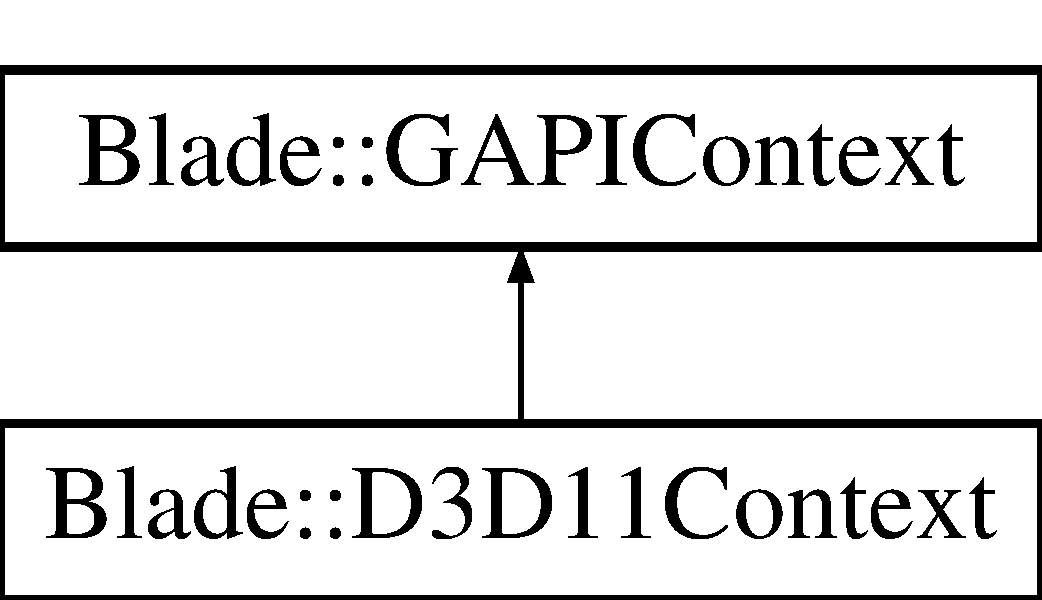
\includegraphics[height=2.000000cm]{class_blade_1_1_g_a_p_i_context}
\end{center}
\end{figure}
\subsection*{Public Member Functions}
\begin{DoxyCompactItemize}
\item 
\mbox{\Hypertarget{class_blade_1_1_g_a_p_i_context_a665c1f1b87abb9128ee009debed3e0e9}\label{class_blade_1_1_g_a_p_i_context_a665c1f1b87abb9128ee009debed3e0e9}} 
virtual bool {\bfseries Create} (L\+U\+ID $\ast$luid)=0
\end{DoxyCompactItemize}


The documentation for this class was generated from the following file\+:\begin{DoxyCompactItemize}
\item 
include/G\+A\+P\+I\+\_\+context.\+h\end{DoxyCompactItemize}

\hypertarget{class_blade_1_1_i_b_o}{}\section{Blade\+:\+:I\+BO Class Reference}
\label{class_blade_1_1_i_b_o}\index{Blade\+::\+I\+BO@{Blade\+::\+I\+BO}}
Inheritance diagram for Blade\+:\+:I\+BO\+:\begin{figure}[H]
\begin{center}
\leavevmode
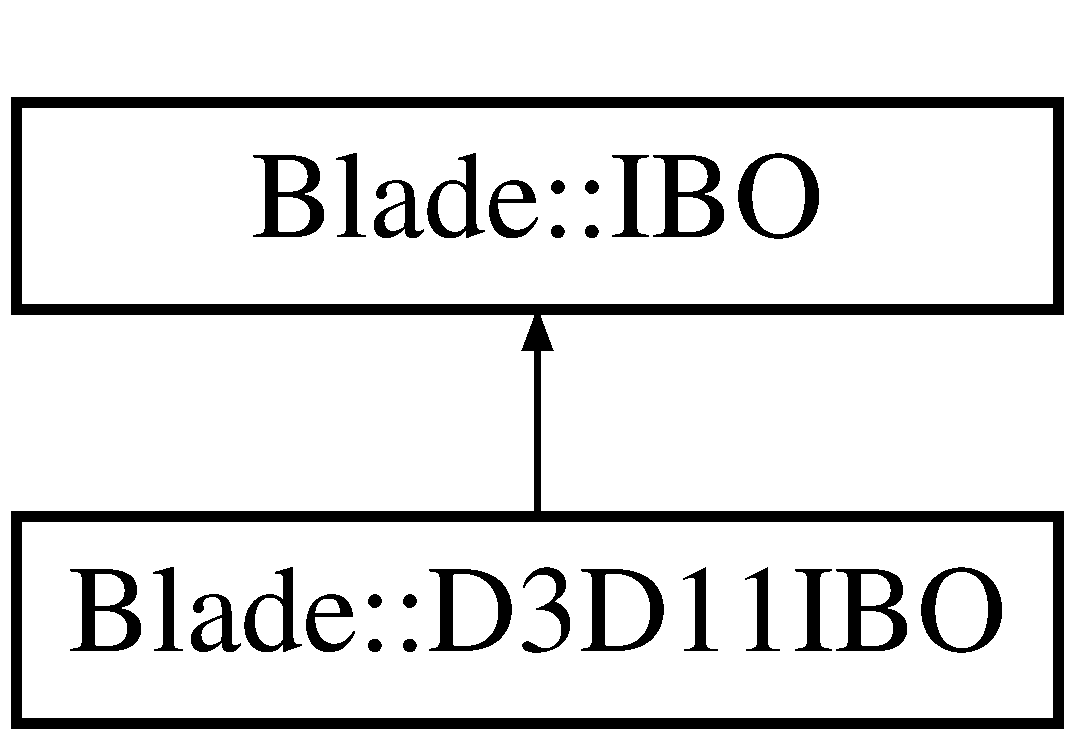
\includegraphics[height=2.000000cm]{class_blade_1_1_i_b_o}
\end{center}
\end{figure}
\subsection*{Public Member Functions}
\begin{DoxyCompactItemize}
\item 
\mbox{\Hypertarget{class_blade_1_1_i_b_o_a46e02fdc0e86623d6fbf46a4b7e378d5}\label{class_blade_1_1_i_b_o_a46e02fdc0e86623d6fbf46a4b7e378d5}} 
void {\bfseries Set\+Index\+Count} (unsigned int idx\+Count) noexcept
\item 
\mbox{\Hypertarget{class_blade_1_1_i_b_o_a2599c509e9f6d5e6428e49c38f64e83d}\label{class_blade_1_1_i_b_o_a2599c509e9f6d5e6428e49c38f64e83d}} 
unsigned int {\bfseries Get\+Index\+Count} () const noexcept
\item 
\mbox{\Hypertarget{class_blade_1_1_i_b_o_afde98cb5cae94bc2f617c74a9fcd5cfe}\label{class_blade_1_1_i_b_o_afde98cb5cae94bc2f617c74a9fcd5cfe}} 
virtual bool {\bfseries Create} (const std\+::vector$<$ unsigned int $>$ \&indices) noexcept=0
\item 
\mbox{\Hypertarget{class_blade_1_1_i_b_o_a1ce875cb7ed5345b64f693908c9a71a4}\label{class_blade_1_1_i_b_o_a1ce875cb7ed5345b64f693908c9a71a4}} 
virtual void {\bfseries Bind} () const noexcept=0
\item 
\mbox{\Hypertarget{class_blade_1_1_i_b_o_ad7875a9e8513fe7f7e20919faa4b5ef3}\label{class_blade_1_1_i_b_o_ad7875a9e8513fe7f7e20919faa4b5ef3}} 
virtual void {\bfseries Draw} () const noexcept=0
\end{DoxyCompactItemize}


The documentation for this class was generated from the following files\+:\begin{DoxyCompactItemize}
\item 
include/I\+B\+O.\+h\item 
src/I\+B\+O.\+cpp\end{DoxyCompactItemize}

\hypertarget{class_blade_1_1_input_component}{}\section{Blade\+:\+:Input\+Component Class Reference}
\label{class_blade_1_1_input_component}\index{Blade\+::\+Input\+Component@{Blade\+::\+Input\+Component}}
Inheritance diagram for Blade\+:\+:Input\+Component\+:\begin{figure}[H]
\begin{center}
\leavevmode
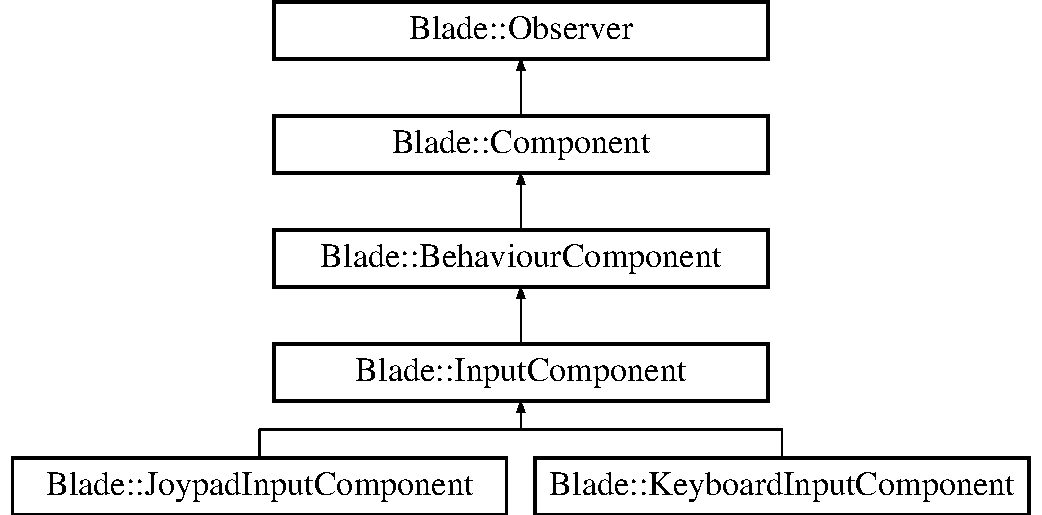
\includegraphics[height=5.000000cm]{class_blade_1_1_input_component}
\end{center}
\end{figure}
\subsection*{Public Member Functions}
\begin{DoxyCompactItemize}
\item 
\mbox{\Hypertarget{class_blade_1_1_input_component_a16ef2c4f95e1597411140ddba84e785e}\label{class_blade_1_1_input_component_a16ef2c4f95e1597411140ddba84e785e}} 
{\bfseries Input\+Component} (const std\+::string \&type, \hyperlink{class_blade_1_1_entity}{Entity} $\ast$parent, bool online=false)
\item 
\mbox{\Hypertarget{class_blade_1_1_input_component_a3ec4713fef0a0903785402a5d6e469ca}\label{class_blade_1_1_input_component_a3ec4713fef0a0903785402a5d6e469ca}} 
{\bfseries Input\+Component} (const \hyperlink{class_blade_1_1_input_component}{Input\+Component} \&other)=delete
\item 
\mbox{\Hypertarget{class_blade_1_1_input_component_a1525696f442c056c06e5018606bf099b}\label{class_blade_1_1_input_component_a1525696f442c056c06e5018606bf099b}} 
\hyperlink{class_blade_1_1_input_component}{Input\+Component} \& {\bfseries operator=} (const \hyperlink{class_blade_1_1_input_component}{Input\+Component} \&other)=delete
\item 
virtual void \hyperlink{class_blade_1_1_input_component_aa7869b52200bb0a8c0c304fdf6147098}{Update} (const float dt, const long time=0) noexcept=0
\begin{DoxyCompactList}\small\item\em Updates the \hyperlink{class_blade_1_1_component}{Component} on each frame. \end{DoxyCompactList}\item 
\mbox{\Hypertarget{class_blade_1_1_input_component_acd17481f4cf26bf9f4bd2c480d97fca1}\label{class_blade_1_1_input_component_acd17481f4cf26bf9f4bd2c480d97fca1}} 
virtual void \hyperlink{class_blade_1_1_input_component_acd17481f4cf26bf9f4bd2c480d97fca1}{Setup} () noexcept=0
\begin{DoxyCompactList}\small\item\em Performs setup actions after the \hyperlink{class_blade_1_1_behaviour_component}{Behaviour\+Component}\textquotesingle{}s creation. \end{DoxyCompactList}\item 
\mbox{\Hypertarget{class_blade_1_1_input_component_aa3f06eb4474d404eb91ab65bad62f4d5}\label{class_blade_1_1_input_component_aa3f06eb4474d404eb91ab65bad62f4d5}} 
virtual void \hyperlink{class_blade_1_1_input_component_aa3f06eb4474d404eb91ab65bad62f4d5}{Teardown} () noexcept=0
\begin{DoxyCompactList}\small\item\em Performs actions before the \hyperlink{class_blade_1_1_behaviour_component}{Behaviour\+Component} is destroyed. \end{DoxyCompactList}\end{DoxyCompactItemize}
\subsection*{Protected Attributes}
\begin{DoxyCompactItemize}
\item 
\mbox{\Hypertarget{class_blade_1_1_input_component_a4b9e54157a5526fb929d5105c4d8447e}\label{class_blade_1_1_input_component_a4b9e54157a5526fb929d5105c4d8447e}} 
bool {\bfseries m\+\_\+\+Online}
\end{DoxyCompactItemize}


\subsection{Member Function Documentation}
\mbox{\Hypertarget{class_blade_1_1_input_component_aa7869b52200bb0a8c0c304fdf6147098}\label{class_blade_1_1_input_component_aa7869b52200bb0a8c0c304fdf6147098}} 
\index{Blade\+::\+Input\+Component@{Blade\+::\+Input\+Component}!Update@{Update}}
\index{Update@{Update}!Blade\+::\+Input\+Component@{Blade\+::\+Input\+Component}}
\subsubsection{\texorpdfstring{Update()}{Update()}}
{\footnotesize\ttfamily virtual void Blade\+::\+Input\+Component\+::\+Update (\begin{DoxyParamCaption}\item[{const float}]{dt,  }\item[{const long}]{time = {\ttfamily 0} }\end{DoxyParamCaption})\hspace{0.3cm}{\ttfamily [pure virtual]}, {\ttfamily [noexcept]}}



Updates the \hyperlink{class_blade_1_1_component}{Component} on each frame. 


\begin{DoxyParams}{Parameters}
{\em dt} & The time elapsed from the previous frame of the \hyperlink{class_blade_1_1_application}{Application}. \\
\hline
{\em time} & The elapsed time since the start of the \hyperlink{class_blade_1_1_application}{Application}. \\
\hline
\end{DoxyParams}


Implements \hyperlink{class_blade_1_1_behaviour_component_a90ec3079534ea1f7225c676881b30c17}{Blade\+::\+Behaviour\+Component}.



Implemented in \hyperlink{class_blade_1_1_joypad_input_component_a386bea7c84d17eefa0d40bfa17575e04}{Blade\+::\+Joypad\+Input\+Component}, and \hyperlink{class_blade_1_1_keyboard_input_component_a0945515e8c0513eaa5b536fd4cb2022c}{Blade\+::\+Keyboard\+Input\+Component}.



The documentation for this class was generated from the following files\+:\begin{DoxyCompactItemize}
\item 
include/input\+\_\+component.\+h\item 
src/input\+\_\+component.\+cpp\end{DoxyCompactItemize}

\hypertarget{class_blade_1_1_input_device}{}\section{Blade\+:\+:Input\+Device Class Reference}
\label{class_blade_1_1_input_device}\index{Blade\+::\+Input\+Device@{Blade\+::\+Input\+Device}}
Inheritance diagram for Blade\+:\+:Input\+Device\+:\begin{figure}[H]
\begin{center}
\leavevmode
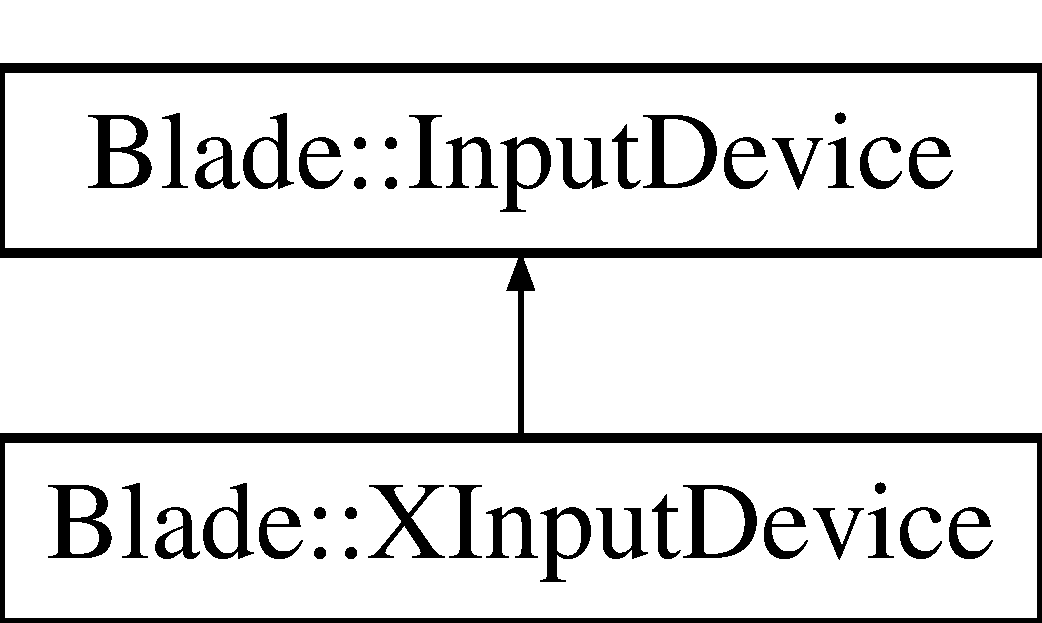
\includegraphics[height=2.000000cm]{class_blade_1_1_input_device}
\end{center}
\end{figure}
\subsection*{Public Member Functions}
\begin{DoxyCompactItemize}
\item 
\mbox{\Hypertarget{class_blade_1_1_input_device_a15fe798555362cbdb43f24d6ffd6c6d5}\label{class_blade_1_1_input_device_a15fe798555362cbdb43f24d6ffd6c6d5}} 
{\bfseries Input\+Device} (const \hyperlink{class_blade_1_1_input_device}{Input\+Device} \&)=delete
\item 
\mbox{\Hypertarget{class_blade_1_1_input_device_a9df7cd958600cc44a020bf92998ac0a6}\label{class_blade_1_1_input_device_a9df7cd958600cc44a020bf92998ac0a6}} 
\hyperlink{class_blade_1_1_input_device}{Input\+Device} \& {\bfseries operator=} (const \hyperlink{class_blade_1_1_input_device}{Input\+Device} \&rhs)=delete
\item 
\mbox{\Hypertarget{class_blade_1_1_input_device_a4c17142daef8c51926d9c77a13c023e2}\label{class_blade_1_1_input_device_a4c17142daef8c51926d9c77a13c023e2}} 
{\bfseries Input\+Device} (\hyperlink{class_blade_1_1_input_device}{Input\+Device} \&\&src)=delete
\item 
\mbox{\Hypertarget{class_blade_1_1_input_device_ac9b63f949dba2011abded48a1237d08f}\label{class_blade_1_1_input_device_ac9b63f949dba2011abded48a1237d08f}} 
\hyperlink{class_blade_1_1_input_device}{Input\+Device} \& {\bfseries operator=} (\hyperlink{class_blade_1_1_input_device}{Input\+Device} \&\&rhs)=delete
\item 
\mbox{\Hypertarget{class_blade_1_1_input_device_a3d54abe984387d8748ff4d8868bb458f}\label{class_blade_1_1_input_device_a3d54abe984387d8748ff4d8868bb458f}} 
{\bfseries Input\+Device} (int device\+\_\+id, Device\+Type dev\+Type)
\item 
\mbox{\Hypertarget{class_blade_1_1_input_device_a0c652079b55274cf661ecf2657f65967}\label{class_blade_1_1_input_device_a0c652079b55274cf661ecf2657f65967}} 
const \hyperlink{struct_blade_1_1_input_state}{Input\+State} \& {\bfseries Get\+Input\+State} () const
\item 
\mbox{\Hypertarget{class_blade_1_1_input_device_af05aace5ac1decaa1bf64bfefbcf013b}\label{class_blade_1_1_input_device_af05aace5ac1decaa1bf64bfefbcf013b}} 
int {\bfseries Get\+Device\+ID} () const
\item 
\mbox{\Hypertarget{class_blade_1_1_input_device_a6c0b653604f7c2a4840116c9e893b3e5}\label{class_blade_1_1_input_device_a6c0b653604f7c2a4840116c9e893b3e5}} 
virtual void {\bfseries Update} (float f\+Delta\+Time)=0
\item 
\mbox{\Hypertarget{class_blade_1_1_input_device_a49858a83478b83d04f95d746cc6a4b75}\label{class_blade_1_1_input_device_a49858a83478b83d04f95d746cc6a4b75}} 
virtual bool {\bfseries Set\+Vibration} (float left\+Motor, float right\+Motor) const =0
\item 
\mbox{\Hypertarget{class_blade_1_1_input_device_a6bb50d40148c2bd07d1b979c4fed8adb}\label{class_blade_1_1_input_device_a6bb50d40148c2bd07d1b979c4fed8adb}} 
void {\bfseries Set\+Deadzone} (Analog\+Deadzone flag, float value)
\item 
\mbox{\Hypertarget{class_blade_1_1_input_device_ab851fc6f3f7f40a376804be9d66a748d}\label{class_blade_1_1_input_device_ab851fc6f3f7f40a376804be9d66a748d}} 
float {\bfseries Get\+Deadzone} (Analog\+Deadzone flag) const
\item 
\mbox{\Hypertarget{class_blade_1_1_input_device_aa9cc6d93af07d3fb28db79f663752c4c}\label{class_blade_1_1_input_device_aa9cc6d93af07d3fb28db79f663752c4c}} 
virtual bool {\bfseries Is\+Connected} () const =0
\item 
\mbox{\Hypertarget{class_blade_1_1_input_device_a4af210da6267e595e1239bab35f8e9e3}\label{class_blade_1_1_input_device_a4af210da6267e595e1239bab35f8e9e3}} 
Device\+Type {\bfseries Get\+Device\+Type} () const
\item 
\mbox{\Hypertarget{class_blade_1_1_input_device_a71a14408ab206c4d983012b06b921d37}\label{class_blade_1_1_input_device_a71a14408ab206c4d983012b06b921d37}} 
const \hyperlink{struct_blade_1_1_input_state}{Input\+State} \& {\bfseries Get\+Current\+State} () const
\item 
\mbox{\Hypertarget{class_blade_1_1_input_device_a45c90dad5932209601cf8eeea85f4036}\label{class_blade_1_1_input_device_a45c90dad5932209601cf8eeea85f4036}} 
const \hyperlink{struct_blade_1_1_input_state}{Input\+State} \& {\bfseries Get\+Previous\+State} () const
\end{DoxyCompactItemize}
\subsection*{Protected Member Functions}
\begin{DoxyCompactItemize}
\item 
\mbox{\Hypertarget{class_blade_1_1_input_device_aa61d2df62fef1370b09ffb7469fc5da4}\label{class_blade_1_1_input_device_aa61d2df62fef1370b09ffb7469fc5da4}} 
void {\bfseries Set\+Device\+ID} (int id)
\item 
\mbox{\Hypertarget{class_blade_1_1_input_device_ab810d1917cee9709b339db1074d10e9a}\label{class_blade_1_1_input_device_ab810d1917cee9709b339db1074d10e9a}} 
void {\bfseries Set\+Device\+Type} (Device\+Type dev\+Type)
\item 
\mbox{\Hypertarget{class_blade_1_1_input_device_a7e01bfa10e141d916b4459051a08b645}\label{class_blade_1_1_input_device_a7e01bfa10e141d916b4459051a08b645}} 
void {\bfseries Set\+Input\+State} (const \hyperlink{struct_blade_1_1_input_state}{Input\+State} \&state)
\item 
\mbox{\Hypertarget{class_blade_1_1_input_device_a701823a23160c1e4e169716647d6570b}\label{class_blade_1_1_input_device_a701823a23160c1e4e169716647d6570b}} 
virtual bool {\bfseries Initialize} ()=0
\end{DoxyCompactItemize}
\subsection*{Static Protected Member Functions}
\begin{DoxyCompactItemize}
\item 
\mbox{\Hypertarget{class_blade_1_1_input_device_ad9d8a25471322063e459f7b13f328d20}\label{class_blade_1_1_input_device_ad9d8a25471322063e459f7b13f328d20}} 
static void {\bfseries Filter\+State\+Data} (const \hyperlink{struct_blade_1_1_input_state}{Input\+State} \&state\+In, \hyperlink{struct_blade_1_1_input_state}{Input\+State} \&state\+Out)
\end{DoxyCompactItemize}


The documentation for this class was generated from the following files\+:\begin{DoxyCompactItemize}
\item 
include/input\+\_\+device.\+h\item 
src/input\+\_\+device.\+cpp\end{DoxyCompactItemize}

\hypertarget{class_blade_1_1_input_manager}{}\section{Blade\+:\+:Input\+Manager Class Reference}
\label{class_blade_1_1_input_manager}\index{Blade\+::\+Input\+Manager@{Blade\+::\+Input\+Manager}}


\hyperlink{class_blade_1_1_input_manager}{Input\+Manager} class of the engine. This class holds and deals with all the external inputs. It supports a polling function to query the current state of a joypad and other helper functions to find the change in states between updates.  




{\ttfamily \#include $<$input\+\_\+manager.\+h$>$}

\subsection*{Public Member Functions}
\begin{DoxyCompactItemize}
\item 
\mbox{\Hypertarget{class_blade_1_1_input_manager_afdd309a456f24335b01544db7d55f400}\label{class_blade_1_1_input_manager_afdd309a456f24335b01544db7d55f400}} 
\hyperlink{class_blade_1_1_input_manager_afdd309a456f24335b01544db7d55f400}{$\sim$\+Input\+Manager} ()
\begin{DoxyCompactList}\small\item\em The input manager destructor. \end{DoxyCompactList}\item 
Vec2f \hyperlink{class_blade_1_1_input_manager_ab41a4d4a8352903e18ba578316c36dc7}{Get\+Analog\+Stick\+Vector} (Joypad\+Number joypad\+Number, \hyperlink{namespace_blade_a1ecca198b7e0afbe43139ec2b0db937c}{Input\+Sensor} sensor)
\begin{DoxyCompactList}\small\item\em Returns a vector indicating the position of the analog stick requested. \end{DoxyCompactList}\item 
bool \hyperlink{class_blade_1_1_input_manager_a8d8e424cb1de012c830296a0812ceebc}{Query\+Key\+State} (\hyperlink{namespace_blade_a15d9bde4921fb2a9a953f8d97ea49d1c}{Virtual\+Key} key) const noexcept
\begin{DoxyCompactList}\small\item\em Query the keyboard device for the state of a key. \end{DoxyCompactList}\item 
bool \hyperlink{class_blade_1_1_input_manager_a6223ce5641fedc88d8e8591deb73ac90}{Query\+All\+Key\+States} (std\+::map$<$ \hyperlink{namespace_blade_a15d9bde4921fb2a9a953f8d97ea49d1c}{Virtual\+Key}, bool $>$ \&dest\+Map) const noexcept
\begin{DoxyCompactList}\small\item\em Query the Keyboard device for the state of A\+LL keys associated to the device. \end{DoxyCompactList}\item 
Vec2f \hyperlink{class_blade_1_1_input_manager_ab1fe795118afeb4642342567d3e27b3f}{Query\+Mouse\+Movement} ()
\begin{DoxyCompactList}\small\item\em Query the Keyboard device for the state of A\+LL keys associated to the device. \end{DoxyCompactList}\item 
Vec2f \hyperlink{class_blade_1_1_input_manager_aa96a587de7ed5234b2b7883df48c0a09}{Query\+Mouse\+Movement\+Normalized} ()
\begin{DoxyCompactList}\small\item\em Query the Keyboard device for the state of A\+LL keys associated to the device. \end{DoxyCompactList}\item 
Vec2i \hyperlink{class_blade_1_1_input_manager_a0bd64dfa38174d3fa87c445ee261d8c3}{Query\+Mouse\+Position} () const noexcept
\begin{DoxyCompactList}\small\item\em Query the Keyboard device for the state of A\+LL keys associated to the device. \end{DoxyCompactList}\item 
bool \hyperlink{class_blade_1_1_input_manager_ad2537487a4c3c80e7eb6b8c0ea37b09b}{Query\+Mouse\+Button\+State} (Mouse\+Button button)
\begin{DoxyCompactList}\small\item\em Query the state of the mouse buttons (providing an enum per button) \end{DoxyCompactList}\item 
bool \hyperlink{class_blade_1_1_input_manager_aeeafae24c87fd12586942eba26956807}{Query\+Device\+State} (Joypad\+Number joypad\+Number, \hyperlink{namespace_blade_a1ecca198b7e0afbe43139ec2b0db937c}{Input\+Sensor} sensor)
\begin{DoxyCompactList}\small\item\em Query the state of a sensor on an active pad linked. \end{DoxyCompactList}\item 
bool \hyperlink{class_blade_1_1_input_manager_ac07153a9c34d35a445ede6c89aa6cbf3}{Query\+Device\+All\+States} (Joypad\+Number joypad\+Number, std\+::map$<$ \hyperlink{namespace_blade_a1ecca198b7e0afbe43139ec2b0db937c}{Input\+Sensor}, bool $>$ \&map)
\begin{DoxyCompactList}\small\item\em Query the input states of sensors on an active device linked to player, return in supplied map. \end{DoxyCompactList}\item 
void \hyperlink{class_blade_1_1_input_manager_a1184a42c2c6b0f96d4169936090f9480}{Update} (float delta\+Time)
\begin{DoxyCompactList}\small\item\em Update the states of managed input devices, and re-\/enumerate input devices. \end{DoxyCompactList}\item 
bool \hyperlink{class_blade_1_1_input_manager_a979db0aea29e22ed95c2642649922a41}{Initialize} () noexcept
\begin{DoxyCompactList}\small\item\em Initialize the input manager. \end{DoxyCompactList}\item 
int \hyperlink{class_blade_1_1_input_manager_afdb7935349eacd9dab51a5b06c8d3864}{Enumerate\+Devices} () noexcept
\begin{DoxyCompactList}\small\item\em Counts and store the number of connected devices to the machine. \end{DoxyCompactList}\item 
Device\+Type \hyperlink{class_blade_1_1_input_manager_a308a056833ddd9aa528ac4fbdbf9df4c}{Device\+Pool\+Query\+Type} (int device\+Id)
\begin{DoxyCompactList}\small\item\em Query a device pool for its type. \end{DoxyCompactList}\item 
bool \hyperlink{class_blade_1_1_input_manager_ae3ccc72d662ee90161206ef64722380f}{Pooled\+Device\+Exists} (int device\+Id)
\begin{DoxyCompactList}\small\item\em Search the device pool for a device with id equal to device\+Id. \end{DoxyCompactList}\item 
bool \hyperlink{class_blade_1_1_input_manager_a6aadb5a4fd8ccfe2de69c1f2d62df37d}{Active\+Device\+Exists} (int device\+Id)
\begin{DoxyCompactList}\small\item\em Search the active device map for a device with id equal to device\+Id. \end{DoxyCompactList}\item 
bool \hyperlink{class_blade_1_1_input_manager_a5369c3110e39e5b3d01349ce7aa676ed}{Assign\+Device\+To\+Player} (Joypad\+Number joypad\+Number, int device\+Number)
\begin{DoxyCompactList}\small\item\em Assigns a player to an input device. \end{DoxyCompactList}\item 
bool \hyperlink{class_blade_1_1_input_manager_ab436b8828eb3022334b544f8e201249e}{Unassign\+Device} (Joypad\+Number joypad\+Number)
\begin{DoxyCompactList}\small\item\em Unassigns an input device from a player (by player ID) \end{DoxyCompactList}\item 
\hyperlink{class_blade_1_1_input_device}{Input\+Device} $\ast$ \hyperlink{class_blade_1_1_input_manager_af7047c9533684d365fb3c61c10911c8c}{Get\+Active\+Device} (Joypad\+Number joypad\+Number)
\begin{DoxyCompactList}\small\item\em Returns an active (not in the pool) assigned input device, searched by player. \end{DoxyCompactList}\item 
void \hyperlink{class_blade_1_1_input_manager_a61209430d6682ade700cc9fa89c7f50e}{Update\+Mouse\+Pos} (Vec2i mousepos)
\begin{DoxyCompactList}\small\item\em Update the position of the mouse. \end{DoxyCompactList}\item 
void \hyperlink{class_blade_1_1_input_manager_a4670405f916ccabf83465154f3649d17}{Set\+Mouse\+Button\+State} (Mouse\+Button state, bool value)
\begin{DoxyCompactList}\small\item\em Update the state of a button of the mouse. \end{DoxyCompactList}\end{DoxyCompactItemize}


\subsection{Detailed Description}
\hyperlink{class_blade_1_1_input_manager}{Input\+Manager} class of the engine. This class holds and deals with all the external inputs. It supports a polling function to query the current state of a joypad and other helper functions to find the change in states between updates. 

\subsection{Member Function Documentation}
\mbox{\Hypertarget{class_blade_1_1_input_manager_a6aadb5a4fd8ccfe2de69c1f2d62df37d}\label{class_blade_1_1_input_manager_a6aadb5a4fd8ccfe2de69c1f2d62df37d}} 
\index{Blade\+::\+Input\+Manager@{Blade\+::\+Input\+Manager}!Active\+Device\+Exists@{Active\+Device\+Exists}}
\index{Active\+Device\+Exists@{Active\+Device\+Exists}!Blade\+::\+Input\+Manager@{Blade\+::\+Input\+Manager}}
\subsubsection{\texorpdfstring{Active\+Device\+Exists()}{ActiveDeviceExists()}}
{\footnotesize\ttfamily bool Blade\+::\+Input\+Manager\+::\+Active\+Device\+Exists (\begin{DoxyParamCaption}\item[{int}]{device\+Id }\end{DoxyParamCaption})}



Search the active device map for a device with id equal to device\+Id. 


\begin{DoxyParams}{Parameters}
{\em device\+Id} & The device number you need to find in the map. \\
\hline
\end{DoxyParams}
\begin{DoxyReturn}{Returns}
True if the device is found, otherwise false 
\end{DoxyReturn}
\mbox{\Hypertarget{class_blade_1_1_input_manager_a5369c3110e39e5b3d01349ce7aa676ed}\label{class_blade_1_1_input_manager_a5369c3110e39e5b3d01349ce7aa676ed}} 
\index{Blade\+::\+Input\+Manager@{Blade\+::\+Input\+Manager}!Assign\+Device\+To\+Player@{Assign\+Device\+To\+Player}}
\index{Assign\+Device\+To\+Player@{Assign\+Device\+To\+Player}!Blade\+::\+Input\+Manager@{Blade\+::\+Input\+Manager}}
\subsubsection{\texorpdfstring{Assign\+Device\+To\+Player()}{AssignDeviceToPlayer()}}
{\footnotesize\ttfamily bool Blade\+::\+Input\+Manager\+::\+Assign\+Device\+To\+Player (\begin{DoxyParamCaption}\item[{Joypad\+Number}]{joypad\+Number,  }\item[{int}]{device\+Number }\end{DoxyParamCaption})}



Assigns a player to an input device. 


\begin{DoxyParams}{Parameters}
{\em joypad\+Number} & The joy pad number. \\
\hline
{\em device\+Number} & The number of the device from the pool. \\
\hline
\end{DoxyParams}
\begin{DoxyReturn}{Returns}
True if successful, false otherwise 
\end{DoxyReturn}
\mbox{\Hypertarget{class_blade_1_1_input_manager_a308a056833ddd9aa528ac4fbdbf9df4c}\label{class_blade_1_1_input_manager_a308a056833ddd9aa528ac4fbdbf9df4c}} 
\index{Blade\+::\+Input\+Manager@{Blade\+::\+Input\+Manager}!Device\+Pool\+Query\+Type@{Device\+Pool\+Query\+Type}}
\index{Device\+Pool\+Query\+Type@{Device\+Pool\+Query\+Type}!Blade\+::\+Input\+Manager@{Blade\+::\+Input\+Manager}}
\subsubsection{\texorpdfstring{Device\+Pool\+Query\+Type()}{DevicePoolQueryType()}}
{\footnotesize\ttfamily Device\+Type Blade\+::\+Input\+Manager\+::\+Device\+Pool\+Query\+Type (\begin{DoxyParamCaption}\item[{int}]{device\+Id }\end{DoxyParamCaption})}



Query a device pool for its type. 


\begin{DoxyParams}{Parameters}
{\em device\+Id} & The device number. \\
\hline
\end{DoxyParams}
\begin{DoxyReturn}{Returns}
Device\+Type enum of the device in the pool denoted by dev\+Index 
\end{DoxyReturn}
\begin{DoxyRemark}{Remarks}
If the device is not found, or an error has occurred, D\+E\+V\+T\+Y\+P\+E\+\_\+\+E\+R\+R\+OR is returned 
\end{DoxyRemark}
\mbox{\Hypertarget{class_blade_1_1_input_manager_afdb7935349eacd9dab51a5b06c8d3864}\label{class_blade_1_1_input_manager_afdb7935349eacd9dab51a5b06c8d3864}} 
\index{Blade\+::\+Input\+Manager@{Blade\+::\+Input\+Manager}!Enumerate\+Devices@{Enumerate\+Devices}}
\index{Enumerate\+Devices@{Enumerate\+Devices}!Blade\+::\+Input\+Manager@{Blade\+::\+Input\+Manager}}
\subsubsection{\texorpdfstring{Enumerate\+Devices()}{EnumerateDevices()}}
{\footnotesize\ttfamily int Blade\+::\+Input\+Manager\+::\+Enumerate\+Devices (\begin{DoxyParamCaption}{ }\end{DoxyParamCaption})\hspace{0.3cm}{\ttfamily [noexcept]}}



Counts and store the number of connected devices to the machine. 

\begin{DoxyReturn}{Returns}
An integer representing the number of connected input devices 
\end{DoxyReturn}
\mbox{\Hypertarget{class_blade_1_1_input_manager_af7047c9533684d365fb3c61c10911c8c}\label{class_blade_1_1_input_manager_af7047c9533684d365fb3c61c10911c8c}} 
\index{Blade\+::\+Input\+Manager@{Blade\+::\+Input\+Manager}!Get\+Active\+Device@{Get\+Active\+Device}}
\index{Get\+Active\+Device@{Get\+Active\+Device}!Blade\+::\+Input\+Manager@{Blade\+::\+Input\+Manager}}
\subsubsection{\texorpdfstring{Get\+Active\+Device()}{GetActiveDevice()}}
{\footnotesize\ttfamily \hyperlink{class_blade_1_1_input_device}{Input\+Device} $\ast$ Blade\+::\+Input\+Manager\+::\+Get\+Active\+Device (\begin{DoxyParamCaption}\item[{Joypad\+Number}]{joypad\+Number }\end{DoxyParamCaption})}



Returns an active (not in the pool) assigned input device, searched by player. 


\begin{DoxyParams}{Parameters}
{\em joypad\+Number} & The number of the joy pad number. \\
\hline
\end{DoxyParams}
\begin{DoxyReturn}{Returns}
Active input device for player id, nullptr otherwise 
\end{DoxyReturn}
\mbox{\Hypertarget{class_blade_1_1_input_manager_ab41a4d4a8352903e18ba578316c36dc7}\label{class_blade_1_1_input_manager_ab41a4d4a8352903e18ba578316c36dc7}} 
\index{Blade\+::\+Input\+Manager@{Blade\+::\+Input\+Manager}!Get\+Analog\+Stick\+Vector@{Get\+Analog\+Stick\+Vector}}
\index{Get\+Analog\+Stick\+Vector@{Get\+Analog\+Stick\+Vector}!Blade\+::\+Input\+Manager@{Blade\+::\+Input\+Manager}}
\subsubsection{\texorpdfstring{Get\+Analog\+Stick\+Vector()}{GetAnalogStickVector()}}
{\footnotesize\ttfamily Vec2f Blade\+::\+Input\+Manager\+::\+Get\+Analog\+Stick\+Vector (\begin{DoxyParamCaption}\item[{Joypad\+Number}]{joypad\+Number,  }\item[{\hyperlink{namespace_blade_a1ecca198b7e0afbe43139ec2b0db937c}{Input\+Sensor}}]{sensor }\end{DoxyParamCaption})}



Returns a vector indicating the position of the analog stick requested. 


\begin{DoxyParams}{Parameters}
{\em joypad\+Number} & The joypad number. \\
\hline
{\em sensor} & The stick that need to be checked \\
\hline
\end{DoxyParams}
\begin{DoxyReturn}{Returns}
The vector that represent the stick position normalized outside dead zones. 
\end{DoxyReturn}
\mbox{\Hypertarget{class_blade_1_1_input_manager_a979db0aea29e22ed95c2642649922a41}\label{class_blade_1_1_input_manager_a979db0aea29e22ed95c2642649922a41}} 
\index{Blade\+::\+Input\+Manager@{Blade\+::\+Input\+Manager}!Initialize@{Initialize}}
\index{Initialize@{Initialize}!Blade\+::\+Input\+Manager@{Blade\+::\+Input\+Manager}}
\subsubsection{\texorpdfstring{Initialize()}{Initialize()}}
{\footnotesize\ttfamily bool Blade\+::\+Input\+Manager\+::\+Initialize (\begin{DoxyParamCaption}{ }\end{DoxyParamCaption})\hspace{0.3cm}{\ttfamily [noexcept]}}



Initialize the input manager. 

\begin{DoxyReturn}{Returns}
True if the initialization is successful, false otherwise 
\end{DoxyReturn}
\mbox{\Hypertarget{class_blade_1_1_input_manager_ae3ccc72d662ee90161206ef64722380f}\label{class_blade_1_1_input_manager_ae3ccc72d662ee90161206ef64722380f}} 
\index{Blade\+::\+Input\+Manager@{Blade\+::\+Input\+Manager}!Pooled\+Device\+Exists@{Pooled\+Device\+Exists}}
\index{Pooled\+Device\+Exists@{Pooled\+Device\+Exists}!Blade\+::\+Input\+Manager@{Blade\+::\+Input\+Manager}}
\subsubsection{\texorpdfstring{Pooled\+Device\+Exists()}{PooledDeviceExists()}}
{\footnotesize\ttfamily bool Blade\+::\+Input\+Manager\+::\+Pooled\+Device\+Exists (\begin{DoxyParamCaption}\item[{int}]{device\+Id }\end{DoxyParamCaption})}



Search the device pool for a device with id equal to device\+Id. 


\begin{DoxyParams}{Parameters}
{\em device\+ID} & The device number. \\
\hline
\end{DoxyParams}
\begin{DoxyReturn}{Returns}
True if the device is found, otherwise false 
\end{DoxyReturn}
\mbox{\Hypertarget{class_blade_1_1_input_manager_a6223ce5641fedc88d8e8591deb73ac90}\label{class_blade_1_1_input_manager_a6223ce5641fedc88d8e8591deb73ac90}} 
\index{Blade\+::\+Input\+Manager@{Blade\+::\+Input\+Manager}!Query\+All\+Key\+States@{Query\+All\+Key\+States}}
\index{Query\+All\+Key\+States@{Query\+All\+Key\+States}!Blade\+::\+Input\+Manager@{Blade\+::\+Input\+Manager}}
\subsubsection{\texorpdfstring{Query\+All\+Key\+States()}{QueryAllKeyStates()}}
{\footnotesize\ttfamily bool Blade\+::\+Input\+Manager\+::\+Query\+All\+Key\+States (\begin{DoxyParamCaption}\item[{std\+::map$<$ \hyperlink{namespace_blade_a15d9bde4921fb2a9a953f8d97ea49d1c}{Virtual\+Key}, bool $>$ \&}]{dest\+Map }\end{DoxyParamCaption}) const\hspace{0.3cm}{\ttfamily [noexcept]}}



Query the Keyboard device for the state of A\+LL keys associated to the device. 


\begin{DoxyParams}{Parameters}
{\em map} & The reference to a map of all keyboard states. \\
\hline
\end{DoxyParams}
\begin{DoxyReturn}{Returns}
True if successful, false otherwise 
\end{DoxyReturn}
\mbox{\Hypertarget{class_blade_1_1_input_manager_ac07153a9c34d35a445ede6c89aa6cbf3}\label{class_blade_1_1_input_manager_ac07153a9c34d35a445ede6c89aa6cbf3}} 
\index{Blade\+::\+Input\+Manager@{Blade\+::\+Input\+Manager}!Query\+Device\+All\+States@{Query\+Device\+All\+States}}
\index{Query\+Device\+All\+States@{Query\+Device\+All\+States}!Blade\+::\+Input\+Manager@{Blade\+::\+Input\+Manager}}
\subsubsection{\texorpdfstring{Query\+Device\+All\+States()}{QueryDeviceAllStates()}}
{\footnotesize\ttfamily bool Blade\+::\+Input\+Manager\+::\+Query\+Device\+All\+States (\begin{DoxyParamCaption}\item[{Joypad\+Number}]{joypad\+Number,  }\item[{std\+::map$<$ \hyperlink{namespace_blade_a1ecca198b7e0afbe43139ec2b0db937c}{Input\+Sensor}, bool $>$ \&}]{map }\end{DoxyParamCaption})}



Query the input states of sensors on an active device linked to player, return in supplied map. 


\begin{DoxyParams}{Parameters}
{\em joypad\+Number} & The queried joypad number. \\
\hline
{\em map} & A reference to a map of the state of the joypad. \\
\hline
\end{DoxyParams}
\begin{DoxyReturn}{Returns}
T\+R\+UE if the Joypad\+Number is active, false otherwise 
\end{DoxyReturn}
\mbox{\Hypertarget{class_blade_1_1_input_manager_aeeafae24c87fd12586942eba26956807}\label{class_blade_1_1_input_manager_aeeafae24c87fd12586942eba26956807}} 
\index{Blade\+::\+Input\+Manager@{Blade\+::\+Input\+Manager}!Query\+Device\+State@{Query\+Device\+State}}
\index{Query\+Device\+State@{Query\+Device\+State}!Blade\+::\+Input\+Manager@{Blade\+::\+Input\+Manager}}
\subsubsection{\texorpdfstring{Query\+Device\+State()}{QueryDeviceState()}}
{\footnotesize\ttfamily bool Blade\+::\+Input\+Manager\+::\+Query\+Device\+State (\begin{DoxyParamCaption}\item[{Joypad\+Number}]{joypad\+Number,  }\item[{\hyperlink{namespace_blade_a1ecca198b7e0afbe43139ec2b0db937c}{Input\+Sensor}}]{sensor }\end{DoxyParamCaption})}



Query the state of a sensor on an active pad linked. 


\begin{DoxyParams}{Parameters}
{\em joypad\+Number} & The queried joypad number \\
\hline
{\em sensor} & The sensor to check \\
\hline
\end{DoxyParams}
\begin{DoxyReturn}{Returns}
T\+R\+UE if the the sensor is active (button pressed, stick out of the deadzone), F\+A\+L\+SE otherwise. 
\end{DoxyReturn}
\mbox{\Hypertarget{class_blade_1_1_input_manager_a8d8e424cb1de012c830296a0812ceebc}\label{class_blade_1_1_input_manager_a8d8e424cb1de012c830296a0812ceebc}} 
\index{Blade\+::\+Input\+Manager@{Blade\+::\+Input\+Manager}!Query\+Key\+State@{Query\+Key\+State}}
\index{Query\+Key\+State@{Query\+Key\+State}!Blade\+::\+Input\+Manager@{Blade\+::\+Input\+Manager}}
\subsubsection{\texorpdfstring{Query\+Key\+State()}{QueryKeyState()}}
{\footnotesize\ttfamily bool Blade\+::\+Input\+Manager\+::\+Query\+Key\+State (\begin{DoxyParamCaption}\item[{\hyperlink{namespace_blade_a15d9bde4921fb2a9a953f8d97ea49d1c}{Virtual\+Key}}]{key }\end{DoxyParamCaption}) const\hspace{0.3cm}{\ttfamily [noexcept]}}



Query the keyboard device for the state of a key. 


\begin{DoxyParams}{Parameters}
{\em key} & A keyboard key. \\
\hline
\end{DoxyParams}
\begin{DoxyReturn}{Returns}
True if the key is a P\+R\+E\+S\+S\+ED state (down), false otherwise 
\end{DoxyReturn}
\mbox{\Hypertarget{class_blade_1_1_input_manager_ad2537487a4c3c80e7eb6b8c0ea37b09b}\label{class_blade_1_1_input_manager_ad2537487a4c3c80e7eb6b8c0ea37b09b}} 
\index{Blade\+::\+Input\+Manager@{Blade\+::\+Input\+Manager}!Query\+Mouse\+Button\+State@{Query\+Mouse\+Button\+State}}
\index{Query\+Mouse\+Button\+State@{Query\+Mouse\+Button\+State}!Blade\+::\+Input\+Manager@{Blade\+::\+Input\+Manager}}
\subsubsection{\texorpdfstring{Query\+Mouse\+Button\+State()}{QueryMouseButtonState()}}
{\footnotesize\ttfamily bool Blade\+::\+Input\+Manager\+::\+Query\+Mouse\+Button\+State (\begin{DoxyParamCaption}\item[{Mouse\+Button}]{button }\end{DoxyParamCaption})}



Query the state of the mouse buttons (providing an enum per button) 


\begin{DoxyParams}{Parameters}
{\em button} & The mouse button \\
\hline
\end{DoxyParams}
\begin{DoxyReturn}{Returns}
True if pressed, false otherwise 
\end{DoxyReturn}
\mbox{\Hypertarget{class_blade_1_1_input_manager_ab1fe795118afeb4642342567d3e27b3f}\label{class_blade_1_1_input_manager_ab1fe795118afeb4642342567d3e27b3f}} 
\index{Blade\+::\+Input\+Manager@{Blade\+::\+Input\+Manager}!Query\+Mouse\+Movement@{Query\+Mouse\+Movement}}
\index{Query\+Mouse\+Movement@{Query\+Mouse\+Movement}!Blade\+::\+Input\+Manager@{Blade\+::\+Input\+Manager}}
\subsubsection{\texorpdfstring{Query\+Mouse\+Movement()}{QueryMouseMovement()}}
{\footnotesize\ttfamily Vec2f Blade\+::\+Input\+Manager\+::\+Query\+Mouse\+Movement (\begin{DoxyParamCaption}{ }\end{DoxyParamCaption})}



Query the Keyboard device for the state of A\+LL keys associated to the device. 

\begin{DoxyReturn}{Returns}
True if successful, false otherwise 
\end{DoxyReturn}
\mbox{\Hypertarget{class_blade_1_1_input_manager_aa96a587de7ed5234b2b7883df48c0a09}\label{class_blade_1_1_input_manager_aa96a587de7ed5234b2b7883df48c0a09}} 
\index{Blade\+::\+Input\+Manager@{Blade\+::\+Input\+Manager}!Query\+Mouse\+Movement\+Normalized@{Query\+Mouse\+Movement\+Normalized}}
\index{Query\+Mouse\+Movement\+Normalized@{Query\+Mouse\+Movement\+Normalized}!Blade\+::\+Input\+Manager@{Blade\+::\+Input\+Manager}}
\subsubsection{\texorpdfstring{Query\+Mouse\+Movement\+Normalized()}{QueryMouseMovementNormalized()}}
{\footnotesize\ttfamily Vec2f Blade\+::\+Input\+Manager\+::\+Query\+Mouse\+Movement\+Normalized (\begin{DoxyParamCaption}{ }\end{DoxyParamCaption})}



Query the Keyboard device for the state of A\+LL keys associated to the device. 

\begin{DoxyReturn}{Returns}
True if successful, false otherwise 
\end{DoxyReturn}
\mbox{\Hypertarget{class_blade_1_1_input_manager_a0bd64dfa38174d3fa87c445ee261d8c3}\label{class_blade_1_1_input_manager_a0bd64dfa38174d3fa87c445ee261d8c3}} 
\index{Blade\+::\+Input\+Manager@{Blade\+::\+Input\+Manager}!Query\+Mouse\+Position@{Query\+Mouse\+Position}}
\index{Query\+Mouse\+Position@{Query\+Mouse\+Position}!Blade\+::\+Input\+Manager@{Blade\+::\+Input\+Manager}}
\subsubsection{\texorpdfstring{Query\+Mouse\+Position()}{QueryMousePosition()}}
{\footnotesize\ttfamily Vec2i Blade\+::\+Input\+Manager\+::\+Query\+Mouse\+Position (\begin{DoxyParamCaption}{ }\end{DoxyParamCaption}) const\hspace{0.3cm}{\ttfamily [noexcept]}}



Query the Keyboard device for the state of A\+LL keys associated to the device. 

\begin{DoxyReturn}{Returns}
True if successful, false otherwise 
\end{DoxyReturn}
\mbox{\Hypertarget{class_blade_1_1_input_manager_a4670405f916ccabf83465154f3649d17}\label{class_blade_1_1_input_manager_a4670405f916ccabf83465154f3649d17}} 
\index{Blade\+::\+Input\+Manager@{Blade\+::\+Input\+Manager}!Set\+Mouse\+Button\+State@{Set\+Mouse\+Button\+State}}
\index{Set\+Mouse\+Button\+State@{Set\+Mouse\+Button\+State}!Blade\+::\+Input\+Manager@{Blade\+::\+Input\+Manager}}
\subsubsection{\texorpdfstring{Set\+Mouse\+Button\+State()}{SetMouseButtonState()}}
{\footnotesize\ttfamily void Blade\+::\+Input\+Manager\+::\+Set\+Mouse\+Button\+State (\begin{DoxyParamCaption}\item[{Mouse\+Button}]{state,  }\item[{bool}]{value }\end{DoxyParamCaption})}



Update the state of a button of the mouse. 


\begin{DoxyParams}{Parameters}
{\em state} & The button of the mouse that has changed (left of right) \\
\hline
{\em value} & The boolean value associate with that flag\+: T\+R\+UE pressed.\\
\hline
\end{DoxyParams}
This method is been called inside the window update loop. \mbox{\Hypertarget{class_blade_1_1_input_manager_ab436b8828eb3022334b544f8e201249e}\label{class_blade_1_1_input_manager_ab436b8828eb3022334b544f8e201249e}} 
\index{Blade\+::\+Input\+Manager@{Blade\+::\+Input\+Manager}!Unassign\+Device@{Unassign\+Device}}
\index{Unassign\+Device@{Unassign\+Device}!Blade\+::\+Input\+Manager@{Blade\+::\+Input\+Manager}}
\subsubsection{\texorpdfstring{Unassign\+Device()}{UnassignDevice()}}
{\footnotesize\ttfamily bool Blade\+::\+Input\+Manager\+::\+Unassign\+Device (\begin{DoxyParamCaption}\item[{Joypad\+Number}]{joypad\+Number }\end{DoxyParamCaption})}



Unassigns an input device from a player (by player ID) 


\begin{DoxyParams}{Parameters}
{\em joypad\+Number} & The number of the joy pad player number. \\
\hline
\end{DoxyParams}
\begin{DoxyReturn}{Returns}
Destroy the association between player and device, and mark device as inactive 
\end{DoxyReturn}
\mbox{\Hypertarget{class_blade_1_1_input_manager_a1184a42c2c6b0f96d4169936090f9480}\label{class_blade_1_1_input_manager_a1184a42c2c6b0f96d4169936090f9480}} 
\index{Blade\+::\+Input\+Manager@{Blade\+::\+Input\+Manager}!Update@{Update}}
\index{Update@{Update}!Blade\+::\+Input\+Manager@{Blade\+::\+Input\+Manager}}
\subsubsection{\texorpdfstring{Update()}{Update()}}
{\footnotesize\ttfamily void Blade\+::\+Input\+Manager\+::\+Update (\begin{DoxyParamCaption}\item[{float}]{delta\+Time }\end{DoxyParamCaption})}



Update the states of managed input devices, and re-\/enumerate input devices. 


\begin{DoxyParams}{Parameters}
{\em delta\+Time} & The delta time. \\
\hline
\end{DoxyParams}
\mbox{\Hypertarget{class_blade_1_1_input_manager_a61209430d6682ade700cc9fa89c7f50e}\label{class_blade_1_1_input_manager_a61209430d6682ade700cc9fa89c7f50e}} 
\index{Blade\+::\+Input\+Manager@{Blade\+::\+Input\+Manager}!Update\+Mouse\+Pos@{Update\+Mouse\+Pos}}
\index{Update\+Mouse\+Pos@{Update\+Mouse\+Pos}!Blade\+::\+Input\+Manager@{Blade\+::\+Input\+Manager}}
\subsubsection{\texorpdfstring{Update\+Mouse\+Pos()}{UpdateMousePos()}}
{\footnotesize\ttfamily void Blade\+::\+Input\+Manager\+::\+Update\+Mouse\+Pos (\begin{DoxyParamCaption}\item[{Vec2i}]{mousepos }\end{DoxyParamCaption})}



Update the position of the mouse. 


\begin{DoxyParams}{Parameters}
{\em mousepos} & A vector that represents the mouse position relative to window.\\
\hline
\end{DoxyParams}
This method is been called inside the window update loop. 

The documentation for this class was generated from the following files\+:\begin{DoxyCompactItemize}
\item 
include/input\+\_\+manager.\+h\item 
src/input\+\_\+manager.\+cpp\end{DoxyCompactItemize}

\hypertarget{struct_blade_1_1_input_state}{}\section{Blade\+:\+:Input\+State Struct Reference}
\label{struct_blade_1_1_input_state}\index{Blade\+::\+Input\+State@{Blade\+::\+Input\+State}}


\hyperlink{struct_blade_1_1_input_state}{Input\+State} describes the current state of a device.  




{\ttfamily \#include $<$input\+\_\+state.\+h$>$}

\subsection*{Public Member Functions}
\begin{DoxyCompactItemize}
\item 
\mbox{\Hypertarget{struct_blade_1_1_input_state_a7761b5ee2008116d690acec154b287f3}\label{struct_blade_1_1_input_state_a7761b5ee2008116d690acec154b287f3}} 
{\bfseries Input\+State} (const \hyperlink{struct_blade_1_1_input_state}{Input\+State} \&src) noexcept=default
\item 
\mbox{\Hypertarget{struct_blade_1_1_input_state_a5422cf146a8983a5d819ecc31f102522}\label{struct_blade_1_1_input_state_a5422cf146a8983a5d819ecc31f102522}} 
\hyperlink{struct_blade_1_1_input_state}{Input\+State} \& {\bfseries operator=} (const \hyperlink{struct_blade_1_1_input_state}{Input\+State} \&rhs) noexcept=default
\item 
\mbox{\Hypertarget{struct_blade_1_1_input_state_acc4172340360db7f2f9b5530196638c2}\label{struct_blade_1_1_input_state_acc4172340360db7f2f9b5530196638c2}} 
{\bfseries Input\+State} (\hyperlink{struct_blade_1_1_input_state}{Input\+State} \&\&src) noexcept=default
\item 
\mbox{\Hypertarget{struct_blade_1_1_input_state_a9a429a9e4359993167e91e2c49fce3a7}\label{struct_blade_1_1_input_state_a9a429a9e4359993167e91e2c49fce3a7}} 
\hyperlink{struct_blade_1_1_input_state}{Input\+State} \& {\bfseries operator=} (\hyperlink{struct_blade_1_1_input_state}{Input\+State} \&\&rhs) noexcept=default
\end{DoxyCompactItemize}
\subsection*{Public Attributes}
\begin{DoxyCompactItemize}
\item 
\mbox{\Hypertarget{struct_blade_1_1_input_state_ab2ce303d432538d83d6797e2b0196a54}\label{struct_blade_1_1_input_state_ab2ce303d432538d83d6797e2b0196a54}} 
int \hyperlink{struct_blade_1_1_input_state_ab2ce303d432538d83d6797e2b0196a54}{digital\+Button\+Data} \{ 0 \}
\begin{DoxyCompactList}\small\item\em The digital button data. \end{DoxyCompactList}\item 
\mbox{\Hypertarget{struct_blade_1_1_input_state_aa67cc30dd00b66ac28e30332fc424796}\label{struct_blade_1_1_input_state_aa67cc30dd00b66ac28e30332fc424796}} 
\hyperlink{struct_blade_1_1_thumb_stick}{Thumb\+Stick} \hyperlink{struct_blade_1_1_input_state_aa67cc30dd00b66ac28e30332fc424796}{stick\+Left} \{ 0 \}
\begin{DoxyCompactList}\small\item\em The left analog stick. \end{DoxyCompactList}\item 
\mbox{\Hypertarget{struct_blade_1_1_input_state_a73a2ab51eb7cbd33f2c75c1c152a2da6}\label{struct_blade_1_1_input_state_a73a2ab51eb7cbd33f2c75c1c152a2da6}} 
\hyperlink{struct_blade_1_1_thumb_stick}{Thumb\+Stick} \hyperlink{struct_blade_1_1_input_state_a73a2ab51eb7cbd33f2c75c1c152a2da6}{stick\+Right} \{ 0 \}
\begin{DoxyCompactList}\small\item\em The right analog stick. \end{DoxyCompactList}\item 
\mbox{\Hypertarget{struct_blade_1_1_input_state_a8db118c60d2f8ec3fcd945fcdccb676d}\label{struct_blade_1_1_input_state_a8db118c60d2f8ec3fcd945fcdccb676d}} 
float \hyperlink{struct_blade_1_1_input_state_a8db118c60d2f8ec3fcd945fcdccb676d}{trigger\+Left} \{ 0.\+0f \}
\begin{DoxyCompactList}\small\item\em The left trigger. \end{DoxyCompactList}\item 
\mbox{\Hypertarget{struct_blade_1_1_input_state_aee406e5fca67a20a0483019150355f87}\label{struct_blade_1_1_input_state_aee406e5fca67a20a0483019150355f87}} 
float \hyperlink{struct_blade_1_1_input_state_aee406e5fca67a20a0483019150355f87}{trigger\+Right} \{ 0.\+0f \}
\begin{DoxyCompactList}\small\item\em The right trigger. \end{DoxyCompactList}\end{DoxyCompactItemize}


\subsection{Detailed Description}
\hyperlink{struct_blade_1_1_input_state}{Input\+State} describes the current state of a device. 

The documentation for this struct was generated from the following files\+:\begin{DoxyCompactItemize}
\item 
include/input\+\_\+state.\+h\item 
src/input\+\_\+state.\+cpp\end{DoxyCompactItemize}

\hypertarget{class_blade_1_1_joypad_input_component}{}\section{Blade\+:\+:Joypad\+Input\+Component Class Reference}
\label{class_blade_1_1_joypad_input_component}\index{Blade\+::\+Joypad\+Input\+Component@{Blade\+::\+Joypad\+Input\+Component}}
Inheritance diagram for Blade\+:\+:Joypad\+Input\+Component\+:\begin{figure}[H]
\begin{center}
\leavevmode
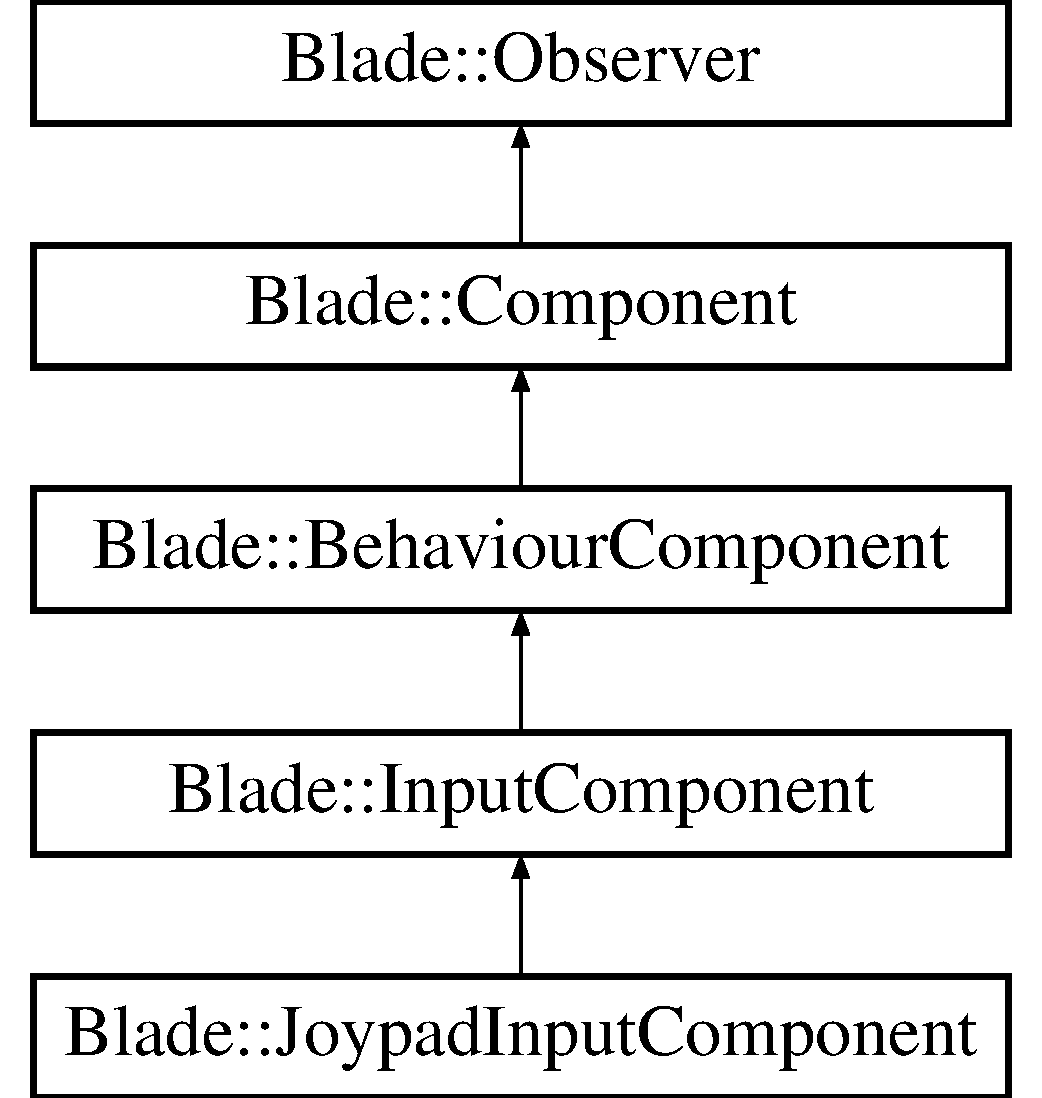
\includegraphics[height=5.000000cm]{class_blade_1_1_joypad_input_component}
\end{center}
\end{figure}
\subsection*{Public Member Functions}
\begin{DoxyCompactItemize}
\item 
\mbox{\Hypertarget{class_blade_1_1_joypad_input_component_a69c169898e9f45399da66f9d912da2cf}\label{class_blade_1_1_joypad_input_component_a69c169898e9f45399da66f9d912da2cf}} 
{\bfseries Joypad\+Input\+Component} (\hyperlink{class_blade_1_1_entity}{Entity} $\ast$parent, Joypad\+Number joypad\+\_\+number, bool online)
\item 
\mbox{\Hypertarget{class_blade_1_1_joypad_input_component_a683bd84cfddc9c0427d673b209feb3a5}\label{class_blade_1_1_joypad_input_component_a683bd84cfddc9c0427d673b209feb3a5}} 
{\bfseries Joypad\+Input\+Component} (const \hyperlink{class_blade_1_1_joypad_input_component}{Joypad\+Input\+Component} \&other)=delete
\item 
\mbox{\Hypertarget{class_blade_1_1_joypad_input_component_a50da9013022078ae5d73a25b3149aad3}\label{class_blade_1_1_joypad_input_component_a50da9013022078ae5d73a25b3149aad3}} 
\hyperlink{class_blade_1_1_joypad_input_component}{Joypad\+Input\+Component} \& {\bfseries operator=} (const \hyperlink{class_blade_1_1_joypad_input_component}{Joypad\+Input\+Component} \&other)=delete
\item 
virtual void \hyperlink{class_blade_1_1_joypad_input_component_a386bea7c84d17eefa0d40bfa17575e04}{Update} (const float dt, const long time=0) noexcept=0
\begin{DoxyCompactList}\small\item\em Updates the \hyperlink{class_blade_1_1_component}{Component} on each frame. \end{DoxyCompactList}\item 
\mbox{\Hypertarget{class_blade_1_1_joypad_input_component_a06b676433645ed509e516061f90589c2}\label{class_blade_1_1_joypad_input_component_a06b676433645ed509e516061f90589c2}} 
virtual void \hyperlink{class_blade_1_1_joypad_input_component_a06b676433645ed509e516061f90589c2}{Setup} () noexcept=0
\begin{DoxyCompactList}\small\item\em Performs setup actions after the \hyperlink{class_blade_1_1_behaviour_component}{Behaviour\+Component}\textquotesingle{}s creation. \end{DoxyCompactList}\item 
\mbox{\Hypertarget{class_blade_1_1_joypad_input_component_ab5009626ea7dd18b3713b4e3ee8fa650}\label{class_blade_1_1_joypad_input_component_ab5009626ea7dd18b3713b4e3ee8fa650}} 
virtual void \hyperlink{class_blade_1_1_joypad_input_component_ab5009626ea7dd18b3713b4e3ee8fa650}{Teardown} () noexcept=0
\begin{DoxyCompactList}\small\item\em Performs actions before the \hyperlink{class_blade_1_1_behaviour_component}{Behaviour\+Component} is destroyed. \end{DoxyCompactList}\item 
\mbox{\Hypertarget{class_blade_1_1_joypad_input_component_aa72a4910f2db050a9d25051e1482b812}\label{class_blade_1_1_joypad_input_component_aa72a4910f2db050a9d25051e1482b812}} 
bool {\bfseries Load\+Configuration} (const std\+::vector$<$ Input\+Sensor $>$ \&control, const std\+::vector$<$ std\+::shared\+\_\+ptr$<$ \hyperlink{class_blade_1_1_command}{Command} $>$$>$ \&commands) noexcept
\item 
\mbox{\Hypertarget{class_blade_1_1_joypad_input_component_a1829016a46492b0e1387db96b5b1ceb0}\label{class_blade_1_1_joypad_input_component_a1829016a46492b0e1387db96b5b1ceb0}} 
bool {\bfseries Load\+Configuration} (const Joypad\+Command\+Map \&map)
\item 
\mbox{\Hypertarget{class_blade_1_1_joypad_input_component_a0835408ffdcf5f6fb44f726f053a7152}\label{class_blade_1_1_joypad_input_component_a0835408ffdcf5f6fb44f726f053a7152}} 
const Joypad\+Command\+Map \& {\bfseries Get\+Command\+Map} () const noexcept
\end{DoxyCompactItemize}
\subsection*{Public Attributes}
\begin{DoxyCompactItemize}
\item 
\mbox{\Hypertarget{class_blade_1_1_joypad_input_component_ad67873042be4c780de3d2257ba2bd88b}\label{class_blade_1_1_joypad_input_component_ad67873042be4c780de3d2257ba2bd88b}} 
Joypad\+Number {\bfseries m\+\_\+\+Joypad\+Num}
\end{DoxyCompactItemize}
\subsection*{Protected Attributes}
\begin{DoxyCompactItemize}
\item 
\mbox{\Hypertarget{class_blade_1_1_joypad_input_component_a17ae33415867c4d3128cfa28f30e46d2}\label{class_blade_1_1_joypad_input_component_a17ae33415867c4d3128cfa28f30e46d2}} 
Joypad\+Command\+Map {\bfseries m\+\_\+\+Joypad\+Command\+Map}
\end{DoxyCompactItemize}


\subsection{Member Function Documentation}
\mbox{\Hypertarget{class_blade_1_1_joypad_input_component_a386bea7c84d17eefa0d40bfa17575e04}\label{class_blade_1_1_joypad_input_component_a386bea7c84d17eefa0d40bfa17575e04}} 
\index{Blade\+::\+Joypad\+Input\+Component@{Blade\+::\+Joypad\+Input\+Component}!Update@{Update}}
\index{Update@{Update}!Blade\+::\+Joypad\+Input\+Component@{Blade\+::\+Joypad\+Input\+Component}}
\subsubsection{\texorpdfstring{Update()}{Update()}}
{\footnotesize\ttfamily virtual void Blade\+::\+Joypad\+Input\+Component\+::\+Update (\begin{DoxyParamCaption}\item[{const float}]{dt,  }\item[{const long}]{time = {\ttfamily 0} }\end{DoxyParamCaption})\hspace{0.3cm}{\ttfamily [pure virtual]}, {\ttfamily [noexcept]}}



Updates the \hyperlink{class_blade_1_1_component}{Component} on each frame. 


\begin{DoxyParams}{Parameters}
{\em dt} & The time elapsed from the previous frame of the \hyperlink{class_blade_1_1_application}{Application}. \\
\hline
{\em time} & The elapsed time since the start of the \hyperlink{class_blade_1_1_application}{Application}. \\
\hline
\end{DoxyParams}


Implements \hyperlink{class_blade_1_1_input_component_aa7869b52200bb0a8c0c304fdf6147098}{Blade\+::\+Input\+Component}.



The documentation for this class was generated from the following files\+:\begin{DoxyCompactItemize}
\item 
include/joypad\+\_\+input\+\_\+component.\+h\item 
src/joypad\+\_\+input\+\_\+component.\+cpp\end{DoxyCompactItemize}

\hypertarget{class_blade_1_1_keyboard_input}{}\section{Blade\+:\+:Keyboard\+Input Class Reference}
\label{class_blade_1_1_keyboard_input}\index{Blade\+::\+Keyboard\+Input@{Blade\+::\+Keyboard\+Input}}


Keyboard abstraction of the engine.  




{\ttfamily \#include $<$keyboard\+\_\+input.\+h$>$}

\subsection*{Static Public Member Functions}
\begin{DoxyCompactItemize}
\item 
static bool \hyperlink{class_blade_1_1_keyboard_input_a9430c44501f4c2a4c3550be2b4bc05d0}{Query\+Key\+State} (Virtual\+Key value) noexcept
\begin{DoxyCompactList}\small\item\em Query the state of a virtual key. \end{DoxyCompactList}\item 
static bool \hyperlink{class_blade_1_1_keyboard_input_acf01cd89bda99e5508dbe7560447651c}{Query\+All\+Key\+States} (std\+::map$<$ Virtual\+Key, bool $>$ \&dest\+Map) noexcept
\begin{DoxyCompactList}\small\item\em Query all virtual key states for attached keyboard. \end{DoxyCompactList}\end{DoxyCompactItemize}


\subsection{Detailed Description}
Keyboard abstraction of the engine. 

\subsection{Member Function Documentation}
\mbox{\Hypertarget{class_blade_1_1_keyboard_input_acf01cd89bda99e5508dbe7560447651c}\label{class_blade_1_1_keyboard_input_acf01cd89bda99e5508dbe7560447651c}} 
\index{Blade\+::\+Keyboard\+Input@{Blade\+::\+Keyboard\+Input}!Query\+All\+Key\+States@{Query\+All\+Key\+States}}
\index{Query\+All\+Key\+States@{Query\+All\+Key\+States}!Blade\+::\+Keyboard\+Input@{Blade\+::\+Keyboard\+Input}}
\subsubsection{\texorpdfstring{Query\+All\+Key\+States()}{QueryAllKeyStates()}}
{\footnotesize\ttfamily bool Blade\+::\+Keyboard\+Input\+::\+Query\+All\+Key\+States (\begin{DoxyParamCaption}\item[{std\+::map$<$ Virtual\+Key, bool $>$ \&}]{dest\+Map }\end{DoxyParamCaption})\hspace{0.3cm}{\ttfamily [static]}, {\ttfamily [noexcept]}}



Query all virtual key states for attached keyboard. 

\begin{DoxyReturn}{Returns}
True if successful, false otherwise 
\end{DoxyReturn}
\mbox{\Hypertarget{class_blade_1_1_keyboard_input_a9430c44501f4c2a4c3550be2b4bc05d0}\label{class_blade_1_1_keyboard_input_a9430c44501f4c2a4c3550be2b4bc05d0}} 
\index{Blade\+::\+Keyboard\+Input@{Blade\+::\+Keyboard\+Input}!Query\+Key\+State@{Query\+Key\+State}}
\index{Query\+Key\+State@{Query\+Key\+State}!Blade\+::\+Keyboard\+Input@{Blade\+::\+Keyboard\+Input}}
\subsubsection{\texorpdfstring{Query\+Key\+State()}{QueryKeyState()}}
{\footnotesize\ttfamily bool Blade\+::\+Keyboard\+Input\+::\+Query\+Key\+State (\begin{DoxyParamCaption}\item[{Virtual\+Key}]{value }\end{DoxyParamCaption})\hspace{0.3cm}{\ttfamily [static]}, {\ttfamily [noexcept]}}



Query the state of a virtual key. 

\begin{DoxyReturn}{Returns}
True if the key being queried is P\+R\+E\+S\+S\+ED (down), false otherwise 
\end{DoxyReturn}


The documentation for this class was generated from the following files\+:\begin{DoxyCompactItemize}
\item 
include/keyboard\+\_\+input.\+h\item 
src/keyboard\+\_\+input.\+cpp\end{DoxyCompactItemize}

\hypertarget{class_blade_1_1_keyboard_input_component}{}\section{Blade\+:\+:Keyboard\+Input\+Component Class Reference}
\label{class_blade_1_1_keyboard_input_component}\index{Blade\+::\+Keyboard\+Input\+Component@{Blade\+::\+Keyboard\+Input\+Component}}
Inheritance diagram for Blade\+:\+:Keyboard\+Input\+Component\+:\begin{figure}[H]
\begin{center}
\leavevmode
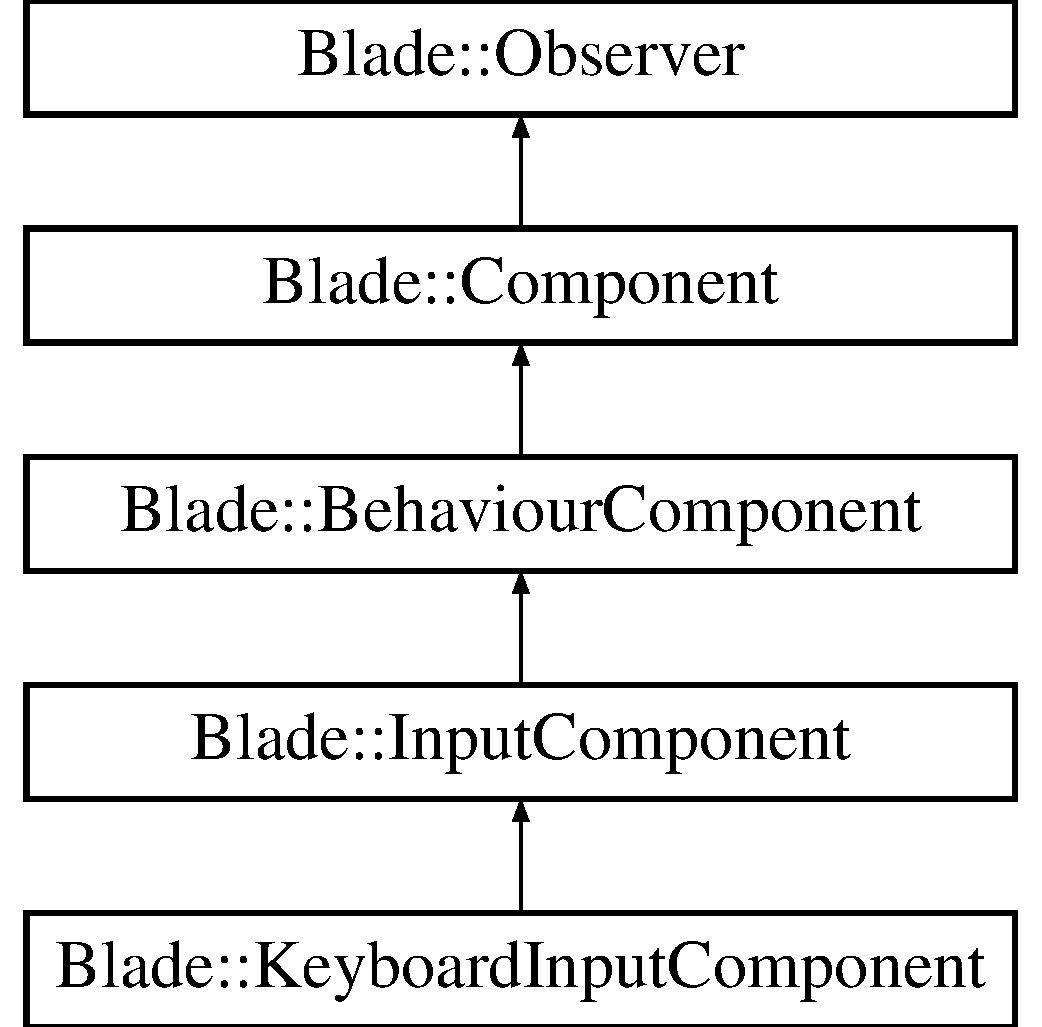
\includegraphics[height=5.000000cm]{class_blade_1_1_keyboard_input_component}
\end{center}
\end{figure}
\subsection*{Public Types}
\begin{DoxyCompactItemize}
\item 
\mbox{\Hypertarget{class_blade_1_1_keyboard_input_component_ae4c93cd11eba12bbf832b25977cd6ff4}\label{class_blade_1_1_keyboard_input_component_ae4c93cd11eba12bbf832b25977cd6ff4}} 
using {\bfseries Keyboard\+Command\+Map} = std\+::map$<$ Virtual\+Key, std\+::shared\+\_\+ptr$<$ \hyperlink{class_blade_1_1_command}{Command} $>$ $>$
\end{DoxyCompactItemize}
\subsection*{Public Member Functions}
\begin{DoxyCompactItemize}
\item 
\mbox{\Hypertarget{class_blade_1_1_keyboard_input_component_aa1cebe940ff791202ee387027071d34b}\label{class_blade_1_1_keyboard_input_component_aa1cebe940ff791202ee387027071d34b}} 
{\bfseries Keyboard\+Input\+Component} (\hyperlink{class_blade_1_1_entity}{Entity} $\ast$parent, bool online)
\item 
\mbox{\Hypertarget{class_blade_1_1_keyboard_input_component_ac63ae86c2904bec43868bb7fea04b8ea}\label{class_blade_1_1_keyboard_input_component_ac63ae86c2904bec43868bb7fea04b8ea}} 
{\bfseries Keyboard\+Input\+Component} (const \hyperlink{class_blade_1_1_keyboard_input_component}{Keyboard\+Input\+Component} \&other)=delete
\item 
\mbox{\Hypertarget{class_blade_1_1_keyboard_input_component_ad67b563f4552bd110e2056966ac843af}\label{class_blade_1_1_keyboard_input_component_ad67b563f4552bd110e2056966ac843af}} 
\hyperlink{class_blade_1_1_keyboard_input_component}{Keyboard\+Input\+Component} \& {\bfseries operator=} (const \hyperlink{class_blade_1_1_keyboard_input_component}{Keyboard\+Input\+Component} \&other)=delete
\item 
virtual void \hyperlink{class_blade_1_1_keyboard_input_component_a0945515e8c0513eaa5b536fd4cb2022c}{Update} (const float dt, const long time=0) noexcept=0
\begin{DoxyCompactList}\small\item\em Updates the \hyperlink{class_blade_1_1_component}{Component} on each frame. \end{DoxyCompactList}\item 
\mbox{\Hypertarget{class_blade_1_1_keyboard_input_component_ae155a4d29a0c1b014b0bc643773aea3f}\label{class_blade_1_1_keyboard_input_component_ae155a4d29a0c1b014b0bc643773aea3f}} 
virtual void \hyperlink{class_blade_1_1_keyboard_input_component_ae155a4d29a0c1b014b0bc643773aea3f}{Setup} () noexcept=0
\begin{DoxyCompactList}\small\item\em Performs setup actions after the \hyperlink{class_blade_1_1_behaviour_component}{Behaviour\+Component}\textquotesingle{}s creation. \end{DoxyCompactList}\item 
\mbox{\Hypertarget{class_blade_1_1_keyboard_input_component_ae62cebd0c5fa0595460275060be472f4}\label{class_blade_1_1_keyboard_input_component_ae62cebd0c5fa0595460275060be472f4}} 
virtual void \hyperlink{class_blade_1_1_keyboard_input_component_ae62cebd0c5fa0595460275060be472f4}{Teardown} () noexcept=0
\begin{DoxyCompactList}\small\item\em Performs actions before the \hyperlink{class_blade_1_1_behaviour_component}{Behaviour\+Component} is destroyed. \end{DoxyCompactList}\item 
\mbox{\Hypertarget{class_blade_1_1_keyboard_input_component_a29dccb52007e5cac972a7af8aee18902}\label{class_blade_1_1_keyboard_input_component_a29dccb52007e5cac972a7af8aee18902}} 
bool {\bfseries Load\+Configuration} (std\+::vector$<$ Virtual\+Key $>$ \&keys, const std\+::vector$<$ std\+::shared\+\_\+ptr$<$ \hyperlink{class_blade_1_1_command}{Command} $>$$>$ \&commands) noexcept
\item 
\mbox{\Hypertarget{class_blade_1_1_keyboard_input_component_ac254b07f58bf9bbe4b936883e113950e}\label{class_blade_1_1_keyboard_input_component_ac254b07f58bf9bbe4b936883e113950e}} 
bool {\bfseries Load\+Configuration} (const Keyboard\+Command\+Map \&map)
\item 
\mbox{\Hypertarget{class_blade_1_1_keyboard_input_component_aae293bcde0e7af3e72e0c5d4ee2fbddc}\label{class_blade_1_1_keyboard_input_component_aae293bcde0e7af3e72e0c5d4ee2fbddc}} 
const Keyboard\+Command\+Map \& {\bfseries Get\+Keyboard\+Command\+Map} () const noexcept
\end{DoxyCompactItemize}
\subsection*{Protected Attributes}
\begin{DoxyCompactItemize}
\item 
\mbox{\Hypertarget{class_blade_1_1_keyboard_input_component_a80b0217398da60a1ccc37609f3c2928d}\label{class_blade_1_1_keyboard_input_component_a80b0217398da60a1ccc37609f3c2928d}} 
Keyboard\+Command\+Map {\bfseries m\+\_\+\+Keyboard\+Command\+Map}
\end{DoxyCompactItemize}


\subsection{Member Function Documentation}
\mbox{\Hypertarget{class_blade_1_1_keyboard_input_component_a0945515e8c0513eaa5b536fd4cb2022c}\label{class_blade_1_1_keyboard_input_component_a0945515e8c0513eaa5b536fd4cb2022c}} 
\index{Blade\+::\+Keyboard\+Input\+Component@{Blade\+::\+Keyboard\+Input\+Component}!Update@{Update}}
\index{Update@{Update}!Blade\+::\+Keyboard\+Input\+Component@{Blade\+::\+Keyboard\+Input\+Component}}
\subsubsection{\texorpdfstring{Update()}{Update()}}
{\footnotesize\ttfamily virtual void Blade\+::\+Keyboard\+Input\+Component\+::\+Update (\begin{DoxyParamCaption}\item[{const float}]{dt,  }\item[{const long}]{time = {\ttfamily 0} }\end{DoxyParamCaption})\hspace{0.3cm}{\ttfamily [pure virtual]}, {\ttfamily [noexcept]}}



Updates the \hyperlink{class_blade_1_1_component}{Component} on each frame. 


\begin{DoxyParams}{Parameters}
{\em dt} & The time elapsed from the previous frame of the \hyperlink{class_blade_1_1_application}{Application}. \\
\hline
{\em time} & The elapsed time since the start of the \hyperlink{class_blade_1_1_application}{Application}. \\
\hline
\end{DoxyParams}


Implements \hyperlink{class_blade_1_1_input_component_aa7869b52200bb0a8c0c304fdf6147098}{Blade\+::\+Input\+Component}.



The documentation for this class was generated from the following files\+:\begin{DoxyCompactItemize}
\item 
include/keyboard\+\_\+input\+\_\+component.\+h\item 
src/keyboard\+\_\+input\+\_\+component.\+cpp\end{DoxyCompactItemize}

\hypertarget{struct_blade_1_1_keyframe}{}\section{Blade\+:\+:Keyframe$<$ T $>$ Struct Template Reference}
\label{struct_blade_1_1_keyframe}\index{Blade\+::\+Keyframe$<$ T $>$@{Blade\+::\+Keyframe$<$ T $>$}}
\subsection*{Public Member Functions}
\begin{DoxyCompactItemize}
\item 
\mbox{\Hypertarget{struct_blade_1_1_keyframe_a4b029db69ce697cd72f56f254fd46d25}\label{struct_blade_1_1_keyframe_a4b029db69ce697cd72f56f254fd46d25}} 
{\bfseries Keyframe} (const T \&value, long time)
\item 
\mbox{\Hypertarget{struct_blade_1_1_keyframe_a09d3923717595ce20fb376e784c54bca}\label{struct_blade_1_1_keyframe_a09d3923717595ce20fb376e784c54bca}} 
bool {\bfseries operator$<$} (const \hyperlink{struct_blade_1_1_keyframe}{Keyframe}$<$ T $>$ \&other) const noexcept
\end{DoxyCompactItemize}
\subsection*{Public Attributes}
\begin{DoxyCompactItemize}
\item 
\mbox{\Hypertarget{struct_blade_1_1_keyframe_a2d896842fbf8bb467a886e5cf84ee963}\label{struct_blade_1_1_keyframe_a2d896842fbf8bb467a886e5cf84ee963}} 
T {\bfseries value}
\item 
\mbox{\Hypertarget{struct_blade_1_1_keyframe_a3cca9ffb7f55931ad5b6a3bf6a23c512}\label{struct_blade_1_1_keyframe_a3cca9ffb7f55931ad5b6a3bf6a23c512}} 
long {\bfseries time} \{ 0 \}
\end{DoxyCompactItemize}


The documentation for this struct was generated from the following file\+:\begin{DoxyCompactItemize}
\item 
include/animation.\+h\end{DoxyCompactItemize}

\hypertarget{class_blade_1_1_light_component}{}\section{Blade\+:\+:Light\+Component Class Reference}
\label{class_blade_1_1_light_component}\index{Blade\+::\+Light\+Component@{Blade\+::\+Light\+Component}}


Abstract class that describes a \hyperlink{class_blade_1_1_light_component}{Light\+Component}. Provides the base functinality of a \hyperlink{class_blade_1_1_light_component}{Light\+Component}. It contains the component\textquotesingle{}s type and an index to the entry of the correct light description cache in the \hyperlink{class_blade_1_1_light_system}{Light\+System}. Managed by the \hyperlink{class_blade_1_1_light_system}{Light\+System}.  




{\ttfamily \#include $<$light\+\_\+component.\+h$>$}

Inheritance diagram for Blade\+:\+:Light\+Component\+:\begin{figure}[H]
\begin{center}
\leavevmode
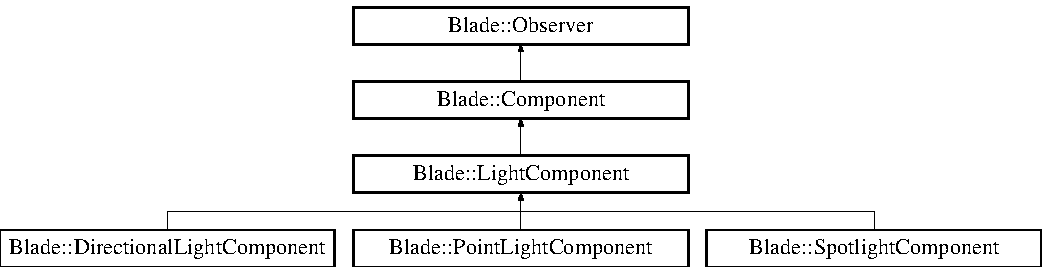
\includegraphics[height=3.572568cm]{class_blade_1_1_light_component}
\end{center}
\end{figure}
\subsection*{Public Member Functions}
\begin{DoxyCompactItemize}
\item 
\mbox{\Hypertarget{class_blade_1_1_light_component_a3dca07977eb7dd2edefebdf6e4cd2da7}\label{class_blade_1_1_light_component_a3dca07977eb7dd2edefebdf6e4cd2da7}} 
{\bfseries Light\+Component} (\hyperlink{namespace_blade_ab0c52aa137a4f43360f7440da56e6b03}{Light\+Type} light\+Type, \hyperlink{class_blade_1_1_entity}{Entity} $\ast$parent)
\item 
\mbox{\Hypertarget{class_blade_1_1_light_component_a1c4113d0e1c0c71501b5e861c46b2eca}\label{class_blade_1_1_light_component_a1c4113d0e1c0c71501b5e861c46b2eca}} 
\hyperlink{namespace_blade_ab0c52aa137a4f43360f7440da56e6b03}{Light\+Type} {\bfseries Get\+Light\+Type} () const noexcept
\item 
\mbox{\Hypertarget{class_blade_1_1_light_component_af6e1c1a417285c8cbef03d6182e8e91c}\label{class_blade_1_1_light_component_af6e1c1a417285c8cbef03d6182e8e91c}} 
int {\bfseries Get\+Light\+Desc\+Cache\+Index} () const noexcept
\item 
\mbox{\Hypertarget{class_blade_1_1_light_component_ab2286335bc867d2f8b98a53cd7ec2123}\label{class_blade_1_1_light_component_ab2286335bc867d2f8b98a53cd7ec2123}} 
void {\bfseries Set\+Light\+Desc\+Cache\+Index} (int index) noexcept
\end{DoxyCompactItemize}


\subsection{Detailed Description}
Abstract class that describes a \hyperlink{class_blade_1_1_light_component}{Light\+Component}. Provides the base functinality of a \hyperlink{class_blade_1_1_light_component}{Light\+Component}. It contains the component\textquotesingle{}s type and an index to the entry of the correct light description cache in the \hyperlink{class_blade_1_1_light_system}{Light\+System}. Managed by the \hyperlink{class_blade_1_1_light_system}{Light\+System}. 

The documentation for this class was generated from the following file\+:\begin{DoxyCompactItemize}
\item 
include/light\+\_\+component.\+h\end{DoxyCompactItemize}

\hypertarget{class_blade_1_1_light_system}{}\section{Blade\+:\+:Light\+System Class Reference}
\label{class_blade_1_1_light_system}\index{Blade\+::\+Light\+System@{Blade\+::\+Light\+System}}


A \hyperlink{class_blade_1_1_system}{System} responsible for managing Light\+Components. This system updates the positions of all the lights in the scene every frame. It is also responsible for caching the light descriptions of each light upon registration of a Light\+Conponent.  




{\ttfamily \#include $<$light\+\_\+system.\+h$>$}

Inheritance diagram for Blade\+:\+:Light\+System\+:\begin{figure}[H]
\begin{center}
\leavevmode
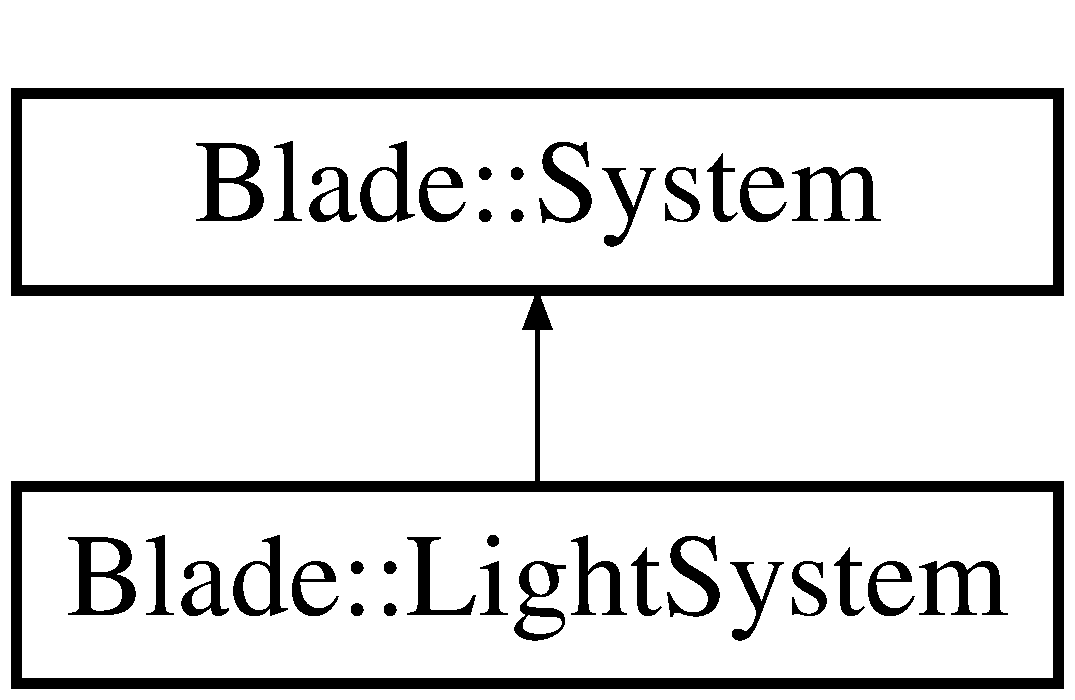
\includegraphics[height=2.000000cm]{class_blade_1_1_light_system}
\end{center}
\end{figure}
\subsection*{Public Member Functions}
\begin{DoxyCompactItemize}
\item 
void \hyperlink{class_blade_1_1_light_system_a0d98342c2927dd165f41ccb50d4845ab}{Register\+Component} (\hyperlink{class_blade_1_1_light_component}{Light\+Component} $\ast$light\+Component) noexcept
\begin{DoxyCompactList}\small\item\em Registers a \hyperlink{class_blade_1_1_light_component}{Light\+Component} to the system. \end{DoxyCompactList}\item 
void \hyperlink{class_blade_1_1_light_system_a7f7a3500b1177ebde379b7fd54b3d16a}{Unregister\+Component} (int id) noexcept
\begin{DoxyCompactList}\small\item\em Unregisters a \hyperlink{class_blade_1_1_light_component}{Light\+Component} from the system. \end{DoxyCompactList}\item 
std\+::vector$<$ \hyperlink{struct_blade_1_1_point_light_desc}{Point\+Light\+Desc} $>$ \hyperlink{class_blade_1_1_light_system_ad42bb7397b56bd224d53425f79c0a63b}{Get\+Point\+Light\+Descriptions} () const noexcept
\begin{DoxyCompactList}\small\item\em Provides a vector of the cached point light description structs. \end{DoxyCompactList}\item 
std\+::vector$<$ \hyperlink{struct_blade_1_1_directional_light_desc}{Directional\+Light\+Desc} $>$ \hyperlink{class_blade_1_1_light_system_a9efaf399620fc75c86fd6032b9291651}{Get\+Directional\+Light\+Descriptions} () const noexcept
\begin{DoxyCompactList}\small\item\em Provides a vector of the cached directional light description structs. \end{DoxyCompactList}\item 
std\+::vector$<$ \hyperlink{struct_blade_1_1_spotlight_desc}{Spotlight\+Desc} $>$ \hyperlink{class_blade_1_1_light_system_ace130c5e66ef2459a8dba36ea448124c}{Get\+Spotlight\+Descriptions} () const noexcept
\begin{DoxyCompactList}\small\item\em Provides a vector of the chached spotlight description structs. \end{DoxyCompactList}\item 
bool \hyperlink{class_blade_1_1_light_system_af87b68ecd946b49576a17e59bfc88934}{Initialize} () noexcept override
\begin{DoxyCompactList}\small\item\em Initialize the Light system. \end{DoxyCompactList}\item 
void \hyperlink{class_blade_1_1_light_system_afbad47302dca40e57322a68252cb08e7}{Process} (float delta\+Time=.\+0f, long time=0) noexcept override
\begin{DoxyCompactList}\small\item\em Processes the Light\+Components. \end{DoxyCompactList}\end{DoxyCompactItemize}


\subsection{Detailed Description}
A \hyperlink{class_blade_1_1_system}{System} responsible for managing Light\+Components. This system updates the positions of all the lights in the scene every frame. It is also responsible for caching the light descriptions of each light upon registration of a Light\+Conponent. 

\subsection{Member Function Documentation}
\mbox{\Hypertarget{class_blade_1_1_light_system_a9efaf399620fc75c86fd6032b9291651}\label{class_blade_1_1_light_system_a9efaf399620fc75c86fd6032b9291651}} 
\index{Blade\+::\+Light\+System@{Blade\+::\+Light\+System}!Get\+Directional\+Light\+Descriptions@{Get\+Directional\+Light\+Descriptions}}
\index{Get\+Directional\+Light\+Descriptions@{Get\+Directional\+Light\+Descriptions}!Blade\+::\+Light\+System@{Blade\+::\+Light\+System}}
\subsubsection{\texorpdfstring{Get\+Directional\+Light\+Descriptions()}{GetDirectionalLightDescriptions()}}
{\footnotesize\ttfamily std\+::vector$<$ \hyperlink{struct_blade_1_1_directional_light_desc}{Directional\+Light\+Desc} $>$ Blade\+::\+Light\+System\+::\+Get\+Directional\+Light\+Descriptions (\begin{DoxyParamCaption}{ }\end{DoxyParamCaption}) const\hspace{0.3cm}{\ttfamily [noexcept]}}



Provides a vector of the cached directional light description structs. 

\begin{DoxyReturn}{Returns}
A vector of the cached directional light description structs. 
\end{DoxyReturn}
\mbox{\Hypertarget{class_blade_1_1_light_system_ad42bb7397b56bd224d53425f79c0a63b}\label{class_blade_1_1_light_system_ad42bb7397b56bd224d53425f79c0a63b}} 
\index{Blade\+::\+Light\+System@{Blade\+::\+Light\+System}!Get\+Point\+Light\+Descriptions@{Get\+Point\+Light\+Descriptions}}
\index{Get\+Point\+Light\+Descriptions@{Get\+Point\+Light\+Descriptions}!Blade\+::\+Light\+System@{Blade\+::\+Light\+System}}
\subsubsection{\texorpdfstring{Get\+Point\+Light\+Descriptions()}{GetPointLightDescriptions()}}
{\footnotesize\ttfamily std\+::vector$<$ \hyperlink{struct_blade_1_1_point_light_desc}{Point\+Light\+Desc} $>$ Blade\+::\+Light\+System\+::\+Get\+Point\+Light\+Descriptions (\begin{DoxyParamCaption}{ }\end{DoxyParamCaption}) const\hspace{0.3cm}{\ttfamily [noexcept]}}



Provides a vector of the cached point light description structs. 

\begin{DoxyReturn}{Returns}
A vector of the cached point light description structs. 
\end{DoxyReturn}
\mbox{\Hypertarget{class_blade_1_1_light_system_ace130c5e66ef2459a8dba36ea448124c}\label{class_blade_1_1_light_system_ace130c5e66ef2459a8dba36ea448124c}} 
\index{Blade\+::\+Light\+System@{Blade\+::\+Light\+System}!Get\+Spotlight\+Descriptions@{Get\+Spotlight\+Descriptions}}
\index{Get\+Spotlight\+Descriptions@{Get\+Spotlight\+Descriptions}!Blade\+::\+Light\+System@{Blade\+::\+Light\+System}}
\subsubsection{\texorpdfstring{Get\+Spotlight\+Descriptions()}{GetSpotlightDescriptions()}}
{\footnotesize\ttfamily std\+::vector$<$ \hyperlink{struct_blade_1_1_spotlight_desc}{Spotlight\+Desc} $>$ Blade\+::\+Light\+System\+::\+Get\+Spotlight\+Descriptions (\begin{DoxyParamCaption}{ }\end{DoxyParamCaption}) const\hspace{0.3cm}{\ttfamily [noexcept]}}



Provides a vector of the chached spotlight description structs. 

\begin{DoxyReturn}{Returns}
A vector of the cached spotlight description structs. 
\end{DoxyReturn}
\mbox{\Hypertarget{class_blade_1_1_light_system_af87b68ecd946b49576a17e59bfc88934}\label{class_blade_1_1_light_system_af87b68ecd946b49576a17e59bfc88934}} 
\index{Blade\+::\+Light\+System@{Blade\+::\+Light\+System}!Initialize@{Initialize}}
\index{Initialize@{Initialize}!Blade\+::\+Light\+System@{Blade\+::\+Light\+System}}
\subsubsection{\texorpdfstring{Initialize()}{Initialize()}}
{\footnotesize\ttfamily bool Blade\+::\+Light\+System\+::\+Initialize (\begin{DoxyParamCaption}{ }\end{DoxyParamCaption})\hspace{0.3cm}{\ttfamily [override]}, {\ttfamily [virtual]}, {\ttfamily [noexcept]}}



Initialize the Light system. 

\begin{DoxyReturn}{Returns}
True if the initialization is successful, false otherwise 
\end{DoxyReturn}


Implements \hyperlink{class_blade_1_1_system_a63fa00af40dc54d093300eff4785f26f}{Blade\+::\+System}.

\mbox{\Hypertarget{class_blade_1_1_light_system_afbad47302dca40e57322a68252cb08e7}\label{class_blade_1_1_light_system_afbad47302dca40e57322a68252cb08e7}} 
\index{Blade\+::\+Light\+System@{Blade\+::\+Light\+System}!Process@{Process}}
\index{Process@{Process}!Blade\+::\+Light\+System@{Blade\+::\+Light\+System}}
\subsubsection{\texorpdfstring{Process()}{Process()}}
{\footnotesize\ttfamily void Blade\+::\+Light\+System\+::\+Process (\begin{DoxyParamCaption}\item[{float}]{delta\+Time = {\ttfamily .0f},  }\item[{long}]{time = {\ttfamily 0} }\end{DoxyParamCaption})\hspace{0.3cm}{\ttfamily [override]}, {\ttfamily [virtual]}, {\ttfamily [noexcept]}}



Processes the Light\+Components. 

This method iterates through all the active Light\+Components. Based on their type it updates the position/direction data members of each \hyperlink{class_blade_1_1_light_component}{Light\+Component}\textquotesingle{}s light description contained in the matching cache. 
\begin{DoxyParams}{Parameters}
{\em delta\+Time} & The time elapsed from the previous frame of the application. \\
\hline
{\em time} & T\+He time since the startup of the application. \\
\hline
\end{DoxyParams}


Implements \hyperlink{class_blade_1_1_system_a80c186f5f9f8fa4fd317b861853fe6a8}{Blade\+::\+System}.

\mbox{\Hypertarget{class_blade_1_1_light_system_a0d98342c2927dd165f41ccb50d4845ab}\label{class_blade_1_1_light_system_a0d98342c2927dd165f41ccb50d4845ab}} 
\index{Blade\+::\+Light\+System@{Blade\+::\+Light\+System}!Register\+Component@{Register\+Component}}
\index{Register\+Component@{Register\+Component}!Blade\+::\+Light\+System@{Blade\+::\+Light\+System}}
\subsubsection{\texorpdfstring{Register\+Component()}{RegisterComponent()}}
{\footnotesize\ttfamily void Blade\+::\+Light\+System\+::\+Register\+Component (\begin{DoxyParamCaption}\item[{\hyperlink{class_blade_1_1_light_component}{Light\+Component} $\ast$}]{light\+Component }\end{DoxyParamCaption})\hspace{0.3cm}{\ttfamily [noexcept]}}



Registers a \hyperlink{class_blade_1_1_light_component}{Light\+Component} to the system. 

This method registers a \hyperlink{class_blade_1_1_light_component}{Light\+Component} to the system. It maps the \hyperlink{class_blade_1_1_light_component}{Light\+Component} with a name and based on it\textquotesingle{}s type it puts the light description contained in the \hyperlink{class_blade_1_1_light_component}{Light\+Component} to the correct light description cache. 
\begin{DoxyParams}{Parameters}
{\em light\+Component} & The \hyperlink{class_blade_1_1_light_component}{Light\+Component} to be registered. \\
\hline
\end{DoxyParams}
\mbox{\Hypertarget{class_blade_1_1_light_system_a7f7a3500b1177ebde379b7fd54b3d16a}\label{class_blade_1_1_light_system_a7f7a3500b1177ebde379b7fd54b3d16a}} 
\index{Blade\+::\+Light\+System@{Blade\+::\+Light\+System}!Unregister\+Component@{Unregister\+Component}}
\index{Unregister\+Component@{Unregister\+Component}!Blade\+::\+Light\+System@{Blade\+::\+Light\+System}}
\subsubsection{\texorpdfstring{Unregister\+Component()}{UnregisterComponent()}}
{\footnotesize\ttfamily void Blade\+::\+Light\+System\+::\+Unregister\+Component (\begin{DoxyParamCaption}\item[{int}]{id }\end{DoxyParamCaption})\hspace{0.3cm}{\ttfamily [noexcept]}}



Unregisters a \hyperlink{class_blade_1_1_light_component}{Light\+Component} from the system. 

This method unregisters a \hyperlink{class_blade_1_1_light_component}{Light\+Component} and based on it\textquotesingle{}s type removes it\textquotesingle{}s light description from the correct light description cache. 
\begin{DoxyParams}{Parameters}
{\em id} & The id of the \hyperlink{class_blade_1_1_light_component}{Light\+Component} to unregister. \\
\hline
\end{DoxyParams}


The documentation for this class was generated from the following files\+:\begin{DoxyCompactItemize}
\item 
include/light\+\_\+system.\+h\item 
src/light\+\_\+system.\+cpp\end{DoxyCompactItemize}

\hypertarget{struct_blade_1_1_manifold_entry}{}\section{Blade\+:\+:Manifold\+Entry Struct Reference}
\label{struct_blade_1_1_manifold_entry}\index{Blade\+::\+Manifold\+Entry@{Blade\+::\+Manifold\+Entry}}
\subsection*{Public Attributes}
\begin{DoxyCompactItemize}
\item 
\mbox{\Hypertarget{struct_blade_1_1_manifold_entry_ac9aa5bc7b2bb1528dacf55a920f7c606}\label{struct_blade_1_1_manifold_entry_ac9aa5bc7b2bb1528dacf55a920f7c606}} 
const \hyperlink{class_blade_1_1_collider}{Collider} $\ast$ {\bfseries collider1}
\item 
\mbox{\Hypertarget{struct_blade_1_1_manifold_entry_aba9ecec3a9f591842930c075c9befb27}\label{struct_blade_1_1_manifold_entry_aba9ecec3a9f591842930c075c9befb27}} 
const \hyperlink{class_blade_1_1_collider}{Collider} $\ast$ {\bfseries collider2}
\item 
\mbox{\Hypertarget{struct_blade_1_1_manifold_entry_a20f40d061764f24ac354cb0ab9f4cb48}\label{struct_blade_1_1_manifold_entry_a20f40d061764f24ac354cb0ab9f4cb48}} 
Vec3f {\bfseries contact\+Normal}
\item 
\mbox{\Hypertarget{struct_blade_1_1_manifold_entry_a88442021e9262b9620528241df4fa0aa}\label{struct_blade_1_1_manifold_entry_a88442021e9262b9620528241df4fa0aa}} 
float {\bfseries t} \{ 0.\+0f \}
\item 
\mbox{\Hypertarget{struct_blade_1_1_manifold_entry_a70040f92b771488762cc5e3e49c9cbf4}\label{struct_blade_1_1_manifold_entry_a70040f92b771488762cc5e3e49c9cbf4}} 
float {\bfseries penetration} \{ 0.\+0f \}
\end{DoxyCompactItemize}


The documentation for this struct was generated from the following file\+:\begin{DoxyCompactItemize}
\item 
include/contact\+\_\+manifold.\+h\end{DoxyCompactItemize}

\hypertarget{struct_blade_1_1_material}{}\section{Blade\+:\+:Material Struct Reference}
\label{struct_blade_1_1_material}\index{Blade\+::\+Material@{Blade\+::\+Material}}
\subsection*{Public Member Functions}
\begin{DoxyCompactItemize}
\item 
\mbox{\Hypertarget{struct_blade_1_1_material_aa30e4a540910d197976f7fdd55d63be4}\label{struct_blade_1_1_material_aa30e4a540910d197976f7fdd55d63be4}} 
{\bfseries Material} (const \hyperlink{struct_blade_1_1_material}{Material} \&other)=default
\item 
\mbox{\Hypertarget{struct_blade_1_1_material_a8fd3dbd8f60be9a87dba3e2c2bf62375}\label{struct_blade_1_1_material_a8fd3dbd8f60be9a87dba3e2c2bf62375}} 
\hyperlink{struct_blade_1_1_material}{Material} \& {\bfseries operator=} (const \hyperlink{struct_blade_1_1_material}{Material} \&other)=default
\end{DoxyCompactItemize}
\subsection*{Public Attributes}
\begin{DoxyCompactItemize}
\item 
\mbox{\Hypertarget{struct_blade_1_1_material_ada13e3f833f05decf7f1d315197a6557}\label{struct_blade_1_1_material_ada13e3f833f05decf7f1d315197a6557}} 
std\+::array$<$ \hyperlink{class_blade_1_1_texture}{Texture} $\ast$, S\+U\+P\+P\+O\+R\+T\+E\+D\+\_\+\+T\+E\+X\+\_\+\+C\+O\+U\+NT $>$ {\bfseries textures}
\item 
\mbox{\Hypertarget{struct_blade_1_1_material_a7355ae3b13d55b8c096741d6776d259e}\label{struct_blade_1_1_material_a7355ae3b13d55b8c096741d6776d259e}} 
Vec4f {\bfseries diffuse}
\item 
\mbox{\Hypertarget{struct_blade_1_1_material_aaaeddb824f6e5e08cf893c4f721033b9}\label{struct_blade_1_1_material_aaaeddb824f6e5e08cf893c4f721033b9}} 
Vec4f {\bfseries specular}
\item 
\mbox{\Hypertarget{struct_blade_1_1_material_aed0395f4111a3c9925fdcdc73d7f7924}\label{struct_blade_1_1_material_aed0395f4111a3c9925fdcdc73d7f7924}} 
Mat4f {\bfseries texture\+Matrix}
\item 
\mbox{\Hypertarget{struct_blade_1_1_material_a98b037e6d19c425274f2e3361cffbc69}\label{struct_blade_1_1_material_a98b037e6d19c425274f2e3361cffbc69}} 
std\+::string {\bfseries shader\+Program\+Name} \{ \char`\"{}sdrprog\+\_\+default\char`\"{} \}
\item 
\mbox{\Hypertarget{struct_blade_1_1_material_a71a20a9776b8b5088521279c7b1a20d9}\label{struct_blade_1_1_material_a71a20a9776b8b5088521279c7b1a20d9}} 
Render\+State\+Type {\bfseries blend\+State}
\end{DoxyCompactItemize}


The documentation for this struct was generated from the following files\+:\begin{DoxyCompactItemize}
\item 
include/material.\+h\item 
src/material.\+cpp\end{DoxyCompactItemize}

\hypertarget{class_blade_1_1_mesh}{}\section{Blade\+:\+:Mesh Class Reference}
\label{class_blade_1_1_mesh}\index{Blade\+::\+Mesh@{Blade\+::\+Mesh}}
Inheritance diagram for Blade\+:\+:Mesh\+:\begin{figure}[H]
\begin{center}
\leavevmode
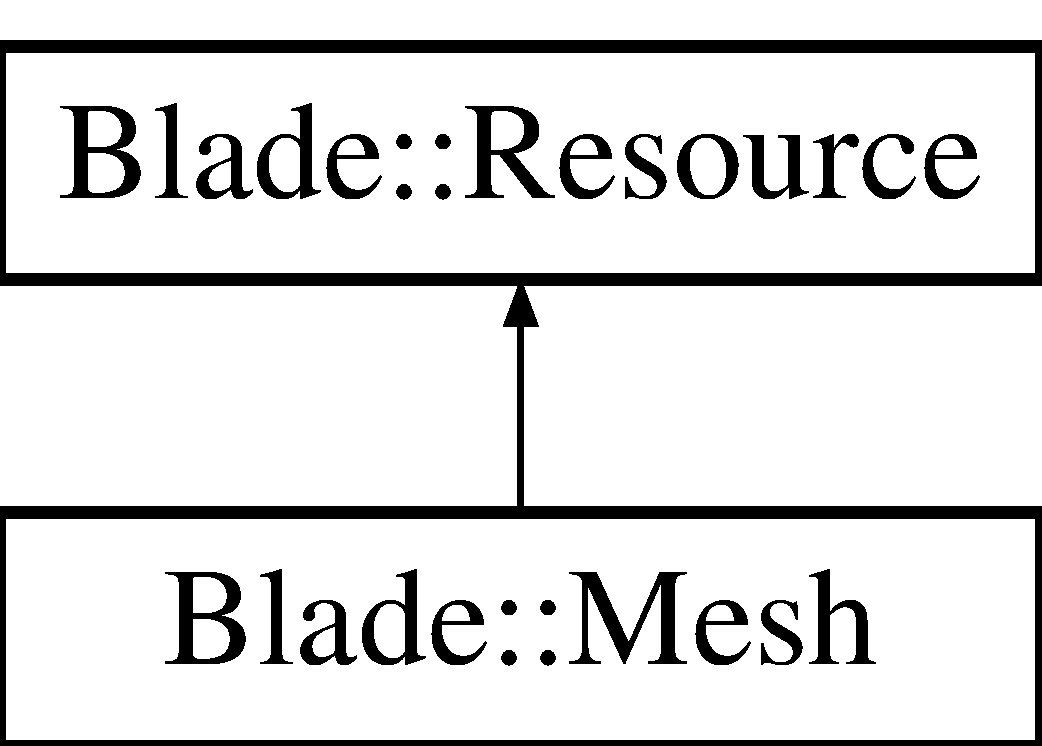
\includegraphics[height=2.000000cm]{class_blade_1_1_mesh}
\end{center}
\end{figure}
\subsection*{Public Member Functions}
\begin{DoxyCompactItemize}
\item 
\mbox{\Hypertarget{class_blade_1_1_mesh_a12f89e6501212e312b12babb4fd59758}\label{class_blade_1_1_mesh_a12f89e6501212e312b12babb4fd59758}} 
{\bfseries Mesh} (const \hyperlink{class_blade_1_1_mesh}{Mesh} \&other)=default
\item 
\mbox{\Hypertarget{class_blade_1_1_mesh_a66fc167597509ce88c82cc874b74eba2}\label{class_blade_1_1_mesh_a66fc167597509ce88c82cc874b74eba2}} 
\hyperlink{class_blade_1_1_mesh}{Mesh} \& {\bfseries operator=} (const \hyperlink{class_blade_1_1_mesh}{Mesh} \&other)=default
\item 
\mbox{\Hypertarget{class_blade_1_1_mesh_ac744768bab4751218d8d045a789cd500}\label{class_blade_1_1_mesh_ac744768bab4751218d8d045a789cd500}} 
\hyperlink{class_blade_1_1_v_b_o}{V\+BO} $\ast$ {\bfseries Get\+Vbo} () const noexcept
\item 
\mbox{\Hypertarget{class_blade_1_1_mesh_a0947f99719a0012972a4fd547c71b217}\label{class_blade_1_1_mesh_a0947f99719a0012972a4fd547c71b217}} 
\hyperlink{class_blade_1_1_i_b_o}{I\+BO} $\ast$ {\bfseries Get\+Ibo} () const noexcept
\item 
\mbox{\Hypertarget{class_blade_1_1_mesh_ae0ba2d92ddf8353d71378206d153cbbf}\label{class_blade_1_1_mesh_ae0ba2d92ddf8353d71378206d153cbbf}} 
size\+\_\+t {\bfseries Get\+Vertex\+Count} () const noexcept
\item 
\mbox{\Hypertarget{class_blade_1_1_mesh_a91e234f58ba1354f0a5d4532cd3162f4}\label{class_blade_1_1_mesh_a91e234f58ba1354f0a5d4532cd3162f4}} 
size\+\_\+t {\bfseries Get\+Index\+Count} () const noexcept
\item 
\mbox{\Hypertarget{class_blade_1_1_mesh_af242f6990adeae394d3049efb38e4e5b}\label{class_blade_1_1_mesh_af242f6990adeae394d3049efb38e4e5b}} 
void {\bfseries Set\+Name} (const std\+::string \&name) noexcept
\item 
\mbox{\Hypertarget{class_blade_1_1_mesh_ad4974970aa0137d481e4233819286bcd}\label{class_blade_1_1_mesh_ad4974970aa0137d481e4233819286bcd}} 
const std\+::string \& {\bfseries Get\+Name} () const noexcept
\item 
\mbox{\Hypertarget{class_blade_1_1_mesh_a39f1b844c2f3b7f804e42241251ee293}\label{class_blade_1_1_mesh_a39f1b844c2f3b7f804e42241251ee293}} 
void {\bfseries Initiaze\+Buffer\+Objects} (Primitive\+Topology primitive\+Topology=Primitive\+Topology\+::\+T\+R\+I\+A\+N\+G\+L\+E\+\_\+\+L\+I\+ST) const noexcept
\item 
\mbox{\Hypertarget{class_blade_1_1_mesh_a7814068ad02de9977c5baf671a6d4cc5}\label{class_blade_1_1_mesh_a7814068ad02de9977c5baf671a6d4cc5}} 
void {\bfseries Set\+Vertex\+Data} (const \hyperlink{struct_blade_1_1_vertex}{Vertex} $\ast$vertices, int vertex\+Count) noexcept
\item 
\mbox{\Hypertarget{class_blade_1_1_mesh_a56d1f9cb6e077fe91eb95452a999f4b3}\label{class_blade_1_1_mesh_a56d1f9cb6e077fe91eb95452a999f4b3}} 
\hyperlink{struct_blade_1_1_vertex}{Vertex} $\ast$ {\bfseries Get\+Vertex\+Data} () const noexcept
\item 
\mbox{\Hypertarget{class_blade_1_1_mesh_a5131c65497cf0dbe611162a86d9bb004}\label{class_blade_1_1_mesh_a5131c65497cf0dbe611162a86d9bb004}} 
void {\bfseries Add\+Vertex} (const \hyperlink{struct_blade_1_1_vertex}{Vertex} \&vertex) noexcept
\item 
\mbox{\Hypertarget{class_blade_1_1_mesh_ad045ba3e642ff52960589372677270fa}\label{class_blade_1_1_mesh_ad045ba3e642ff52960589372677270fa}} 
void {\bfseries Set\+Index\+Data} (const unsigned int $\ast$indices, int index\+Count) noexcept
\item 
\mbox{\Hypertarget{class_blade_1_1_mesh_ac0890adc16e7d52924ccd6ba8f5a2916}\label{class_blade_1_1_mesh_ac0890adc16e7d52924ccd6ba8f5a2916}} 
unsigned int $\ast$ {\bfseries Get\+Index\+Data} () const noexcept
\item 
\mbox{\Hypertarget{class_blade_1_1_mesh_a1c77eda2ea16ed8ebeb74dc97dfc2df8}\label{class_blade_1_1_mesh_a1c77eda2ea16ed8ebeb74dc97dfc2df8}} 
void {\bfseries Add\+Index} (unsigned int index) noexcept
\item 
bool \hyperlink{class_blade_1_1_mesh_a999b87101e849d8a6618d95c69387ec1}{Load} (const std\+::wstring \&file\+Name) noexcept override
\begin{DoxyCompactList}\small\item\em Load a resource form a file. \end{DoxyCompactList}\item 
\mbox{\Hypertarget{class_blade_1_1_mesh_ae9a08be7c3e4c6f6877d99bae35811b6}\label{class_blade_1_1_mesh_ae9a08be7c3e4c6f6877d99bae35811b6}} 
void {\bfseries Generate\+Indices} (Vertex\+Winding winding) noexcept
\end{DoxyCompactItemize}


\subsection{Member Function Documentation}
\mbox{\Hypertarget{class_blade_1_1_mesh_a999b87101e849d8a6618d95c69387ec1}\label{class_blade_1_1_mesh_a999b87101e849d8a6618d95c69387ec1}} 
\index{Blade\+::\+Mesh@{Blade\+::\+Mesh}!Load@{Load}}
\index{Load@{Load}!Blade\+::\+Mesh@{Blade\+::\+Mesh}}
\subsubsection{\texorpdfstring{Load()}{Load()}}
{\footnotesize\ttfamily bool Blade\+::\+Mesh\+::\+Load (\begin{DoxyParamCaption}\item[{const std\+::wstring \&}]{file\+\_\+name }\end{DoxyParamCaption})\hspace{0.3cm}{\ttfamily [override]}, {\ttfamily [virtual]}, {\ttfamily [noexcept]}}



Load a resource form a file. 


\begin{DoxyParams}{Parameters}
{\em file\+\_\+name} & The path of the file where the resource is stored. \\
\hline
\end{DoxyParams}
\begin{DoxyReturn}{Returns}
T\+R\+UE if the loading has been successful, false otherwise. 
\end{DoxyReturn}


Implements \hyperlink{class_blade_1_1_resource_ad89ab00a3b81df1338a8310ec92c5cff}{Blade\+::\+Resource}.



The documentation for this class was generated from the following files\+:\begin{DoxyCompactItemize}
\item 
include/mesh.\+h\item 
src/mesh.\+cpp\end{DoxyCompactItemize}

\hypertarget{class_blade_1_1_message}{}\section{Blade\+:\+:Message$<$ T $>$ Class Template Reference}
\label{class_blade_1_1_message}\index{Blade\+::\+Message$<$ T $>$@{Blade\+::\+Message$<$ T $>$}}
\subsection*{Public Member Functions}
\begin{DoxyCompactItemize}
\item 
\mbox{\Hypertarget{class_blade_1_1_message_a8ffc93ea0c8ab92ce3fabc98d43ec9a1}\label{class_blade_1_1_message_a8ffc93ea0c8ab92ce3fabc98d43ec9a1}} 
{\bfseries Message} (T \&\&type)
\item 
\mbox{\Hypertarget{class_blade_1_1_message_ab47922d6a73d5d01f8f740a926cef656}\label{class_blade_1_1_message_ab47922d6a73d5d01f8f740a926cef656}} 
const T \& {\bfseries Get\+Type} () const noexcept
\end{DoxyCompactItemize}


The documentation for this class was generated from the following file\+:\begin{DoxyCompactItemize}
\item 
include/message.\+h\end{DoxyCompactItemize}

\hypertarget{class_blade_1_1_n_c_f}{}\section{Blade\+:\+:N\+CF Class Reference}
\label{class_blade_1_1_n_c_f}\index{Blade\+::\+N\+CF@{Blade\+::\+N\+CF}}
\subsection*{Public Member Functions}
\begin{DoxyCompactItemize}
\item 
\mbox{\Hypertarget{class_blade_1_1_n_c_f_aec283741da4292cfb5f8d2d637575621}\label{class_blade_1_1_n_c_f_aec283741da4292cfb5f8d2d637575621}} 
void {\bfseries Set\+Source} (const char $\ast$file)
\item 
\mbox{\Hypertarget{class_blade_1_1_n_c_f_a80e322e0d7afa6d5a1b30fa72c6390f5}\label{class_blade_1_1_n_c_f_a80e322e0d7afa6d5a1b30fa72c6390f5}} 
const char $\ast$ {\bfseries Get\+Source} () const
\item 
\mbox{\Hypertarget{class_blade_1_1_n_c_f_a8da4da2db1d461a702da7f393549653a}\label{class_blade_1_1_n_c_f_a8da4da2db1d461a702da7f393549653a}} 
void {\bfseries Purge} ()
\item 
\mbox{\Hypertarget{class_blade_1_1_n_c_f_a7bb935bc00fbd3148fe2c1a5e4ed6e70}\label{class_blade_1_1_n_c_f_a7bb935bc00fbd3148fe2c1a5e4ed6e70}} 
int {\bfseries Parse} ()
\item 
\mbox{\Hypertarget{class_blade_1_1_n_c_f_a8115afecc76f5c5394c01f9b7f3f3c61}\label{class_blade_1_1_n_c_f_a8115afecc76f5c5394c01f9b7f3f3c61}} 
int {\bfseries Dump} (const char $\ast$file, int create=1) const
\item 
\mbox{\Hypertarget{class_blade_1_1_n_c_f_a6326fa802fc4f1d37a1ff70b20bcb9c2}\label{class_blade_1_1_n_c_f_a6326fa802fc4f1d37a1ff70b20bcb9c2}} 
bool {\bfseries Query\+Property} (const char $\ast$name) const
\item 
\mbox{\Hypertarget{class_blade_1_1_n_c_f_a5d11ae00c0f180d63f1e9e2f99dddf29}\label{class_blade_1_1_n_c_f_a5d11ae00c0f180d63f1e9e2f99dddf29}} 
bool {\bfseries Query\+Group} (const char $\ast$name) const
\item 
\mbox{\Hypertarget{class_blade_1_1_n_c_f_a1beb9b88925a9efed0946a7beaa48285}\label{class_blade_1_1_n_c_f_a1beb9b88925a9efed0946a7beaa48285}} 
unsigned int {\bfseries Count\+Properties} () const
\item 
\mbox{\Hypertarget{class_blade_1_1_n_c_f_afbf5dba9744140317952292c92f99874}\label{class_blade_1_1_n_c_f_afbf5dba9744140317952292c92f99874}} 
unsigned int {\bfseries Count\+Groups} () const
\item 
\mbox{\Hypertarget{class_blade_1_1_n_c_f_aca49d89ab36e6233da20cb89ebfba03f}\label{class_blade_1_1_n_c_f_aca49d89ab36e6233da20cb89ebfba03f}} 
void {\bfseries Set\+Property} (const char $\ast$name, const char $\ast$value)
\item 
\mbox{\Hypertarget{class_blade_1_1_n_c_f_afc76559d747e2ff4a790e41f27317773}\label{class_blade_1_1_n_c_f_afc76559d747e2ff4a790e41f27317773}} 
const char $\ast$ {\bfseries Get\+Property\+By\+Name} (const char $\ast$name) const
\item 
\mbox{\Hypertarget{class_blade_1_1_n_c_f_a2cbbea6126f06913ff3ddabaa0d3a0a8}\label{class_blade_1_1_n_c_f_a2cbbea6126f06913ff3ddabaa0d3a0a8}} 
const char $\ast$ {\bfseries Get\+Property\+By\+Index} (unsigned int index) const
\item 
\mbox{\Hypertarget{class_blade_1_1_n_c_f_afa56a28ff9b12f922c51fe2baf7eed50}\label{class_blade_1_1_n_c_f_afa56a28ff9b12f922c51fe2baf7eed50}} 
const char $\ast$ {\bfseries Get\+Property\+Name\+By\+Index} (unsigned int index) const
\item 
\mbox{\Hypertarget{class_blade_1_1_n_c_f_a956eca2a28ecf9f02e707610f2023893}\label{class_blade_1_1_n_c_f_a956eca2a28ecf9f02e707610f2023893}} 
\hyperlink{class_blade_1_1_n_c_f}{N\+CF} $\ast$ {\bfseries Get\+Group\+By\+Name} (const char $\ast$name) const
\item 
\mbox{\Hypertarget{class_blade_1_1_n_c_f_a6c9b4eff03b22bd7209a26e687fd8c39}\label{class_blade_1_1_n_c_f_a6c9b4eff03b22bd7209a26e687fd8c39}} 
\hyperlink{class_blade_1_1_n_c_f}{N\+CF} $\ast$ {\bfseries Get\+Group\+By\+Index} (unsigned int index) const
\item 
\mbox{\Hypertarget{class_blade_1_1_n_c_f_aae88a3edcbc65daed7031c33dae14326}\label{class_blade_1_1_n_c_f_aae88a3edcbc65daed7031c33dae14326}} 
const char $\ast$ {\bfseries Get\+Name} () const
\item 
\mbox{\Hypertarget{class_blade_1_1_n_c_f_af6c4e7db67263bca7c6222f30481c4c5}\label{class_blade_1_1_n_c_f_af6c4e7db67263bca7c6222f30481c4c5}} 
{\bfseries N\+CF} (const \hyperlink{class_blade_1_1_n_c_f}{N\+CF} \&)=delete
\item 
\mbox{\Hypertarget{class_blade_1_1_n_c_f_af9c0395ef323de8a3a832f7a4b189339}\label{class_blade_1_1_n_c_f_af9c0395ef323de8a3a832f7a4b189339}} 
\hyperlink{class_blade_1_1_n_c_f}{N\+CF} \& {\bfseries operator=} (const \hyperlink{class_blade_1_1_n_c_f}{N\+CF} \&)=delete
\end{DoxyCompactItemize}


The documentation for this class was generated from the following files\+:\begin{DoxyCompactItemize}
\item 
include/ncf.\+h\item 
src/ncf.\+cpp\end{DoxyCompactItemize}

\hypertarget{class_blade_1_1_network_manager}{}\section{Blade\+:\+:Network\+Manager Class Reference}
\label{class_blade_1_1_network_manager}\index{Blade\+::\+Network\+Manager@{Blade\+::\+Network\+Manager}}
\subsection*{Public Member Functions}
\begin{DoxyCompactItemize}
\item 
\mbox{\Hypertarget{class_blade_1_1_network_manager_a9b1c863473df3dddfd4347c4fa570a80}\label{class_blade_1_1_network_manager_a9b1c863473df3dddfd4347c4fa570a80}} 
bool {\bfseries Initialize} () noexcept
\item 
\mbox{\Hypertarget{class_blade_1_1_network_manager_a1e097a251026499832bd7238adb48d8a}\label{class_blade_1_1_network_manager_a1e097a251026499832bd7238adb48d8a}} 
void {\bfseries Listen} (const unsigned short port) noexcept
\item 
\mbox{\Hypertarget{class_blade_1_1_network_manager_a61a872d6eec9050280dc041a7cda3759}\label{class_blade_1_1_network_manager_a61a872d6eec9050280dc041a7cda3759}} 
void {\bfseries Connect} (const std\+::string \&host, const unsigned short port) noexcept
\item 
\mbox{\Hypertarget{class_blade_1_1_network_manager_a3127ee70f644dedfa8be9372805f6d5a}\label{class_blade_1_1_network_manager_a3127ee70f644dedfa8be9372805f6d5a}} 
void {\bfseries Queue\+Message} (const std\+::shared\+\_\+ptr$<$ \hyperlink{class_blade_1_1_network_message}{Network\+Message} $>$ \&message) noexcept
\item 
\mbox{\Hypertarget{class_blade_1_1_network_manager_ac8dcbba66d285f6a14ad1bcfa346ae5e}\label{class_blade_1_1_network_manager_ac8dcbba66d285f6a14ad1bcfa346ae5e}} 
size\+\_\+t {\bfseries Get\+Connection\+Count} () noexcept
\item 
\mbox{\Hypertarget{class_blade_1_1_network_manager_a12f5afdfc075b71ea82d4d657a78d780}\label{class_blade_1_1_network_manager_a12f5afdfc075b71ea82d4d657a78d780}} 
void {\bfseries Set\+On\+New\+Packet\+Callback} (const On\+New\+Packet\+Callback \&callback) noexcept
\item 
\mbox{\Hypertarget{class_blade_1_1_network_manager_a192f822f26e76829c2414f1505418a78}\label{class_blade_1_1_network_manager_a192f822f26e76829c2414f1505418a78}} 
void {\bfseries Set\+On\+New\+Client\+Callback} (const On\+New\+Client\+Callback \&callback) noexcept
\item 
\mbox{\Hypertarget{class_blade_1_1_network_manager_ada4cd3f291d3775e7467c5be31090a99}\label{class_blade_1_1_network_manager_ada4cd3f291d3775e7467c5be31090a99}} 
void {\bfseries Set\+On\+Client\+Disconnect\+Callback} (const On\+Client\+Disconnect\+Callback \&callback) noexcept
\end{DoxyCompactItemize}


The documentation for this class was generated from the following files\+:\begin{DoxyCompactItemize}
\item 
include/network\+\_\+manager.\+h\item 
src/network\+\_\+manager.\+cpp\end{DoxyCompactItemize}

\hypertarget{class_blade_1_1_network_message}{}\section{Blade\+:\+:Network\+Message Class Reference}
\label{class_blade_1_1_network_message}\index{Blade\+::\+Network\+Message@{Blade\+::\+Network\+Message}}
Inheritance diagram for Blade\+:\+:Network\+Message\+:\begin{figure}[H]
\begin{center}
\leavevmode
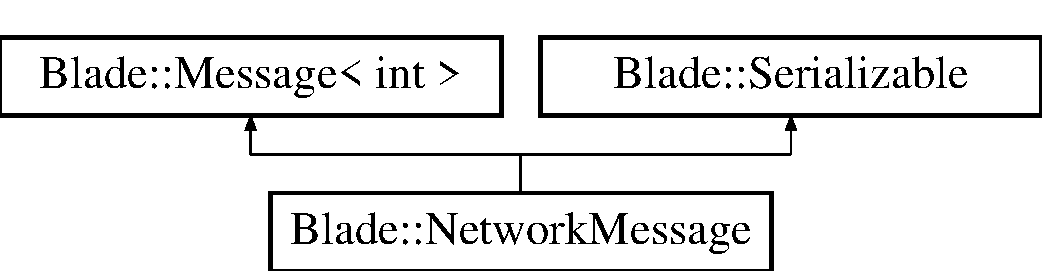
\includegraphics[height=2.000000cm]{class_blade_1_1_network_message}
\end{center}
\end{figure}
\subsection*{Public Member Functions}
\begin{DoxyCompactItemize}
\item 
\mbox{\Hypertarget{class_blade_1_1_network_message_a4711d53f8f0df27056b814b7eca31efc}\label{class_blade_1_1_network_message_a4711d53f8f0df27056b814b7eca31efc}} 
{\bfseries Network\+Message} (int \&\&type, long recipient\+Id)
\end{DoxyCompactItemize}


The documentation for this class was generated from the following file\+:\begin{DoxyCompactItemize}
\item 
include/network\+\_\+message.\+h\end{DoxyCompactItemize}

\hypertarget{class_blade_1_1_observer}{}\section{Blade\+:\+:Observer Class Reference}
\label{class_blade_1_1_observer}\index{Blade\+::\+Observer@{Blade\+::\+Observer}}


\hyperlink{class_blade_1_1_observer}{Observer} class of the engine.  




{\ttfamily \#include $<$observer.\+h$>$}

Inheritance diagram for Blade\+:\+:Observer\+:\begin{figure}[H]
\begin{center}
\leavevmode
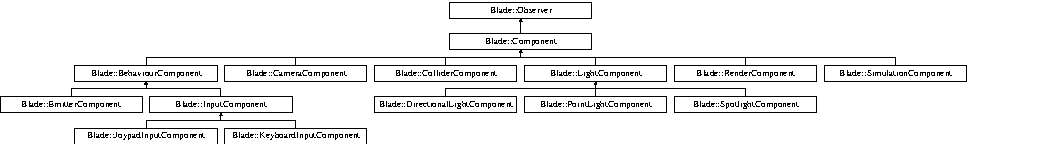
\includegraphics[height=1.913875cm]{class_blade_1_1_observer}
\end{center}
\end{figure}
\subsection*{Public Member Functions}
\begin{DoxyCompactItemize}
\item 
\mbox{\Hypertarget{class_blade_1_1_observer_acbb85f46b9cd5c60e4c7b8ebb7dc4faa}\label{class_blade_1_1_observer_acbb85f46b9cd5c60e4c7b8ebb7dc4faa}} 
virtual void {\bfseries On\+Message} (const \hyperlink{class_blade_1_1_ref_counted_container}{Message\+Container}$<$ std\+::string $>$ \&msg)=0
\end{DoxyCompactItemize}


\subsection{Detailed Description}
\hyperlink{class_blade_1_1_observer}{Observer} class of the engine. 

The engine provides observer pattern interface 

The documentation for this class was generated from the following files\+:\begin{DoxyCompactItemize}
\item 
include/observer.\+h\item 
src/observer.\+cpp\end{DoxyCompactItemize}

\hypertarget{class_blade_1_1_observer_subject}{}\section{Blade\+:\+:Observer\+Subject Class Reference}
\label{class_blade_1_1_observer_subject}\index{Blade\+::\+Observer\+Subject@{Blade\+::\+Observer\+Subject}}


Objeserver\+Subject implemented by the engine.  




{\ttfamily \#include $<$observer\+\_\+subject.\+h$>$}

Inheritance diagram for Blade\+:\+:Observer\+Subject\+:\begin{figure}[H]
\begin{center}
\leavevmode
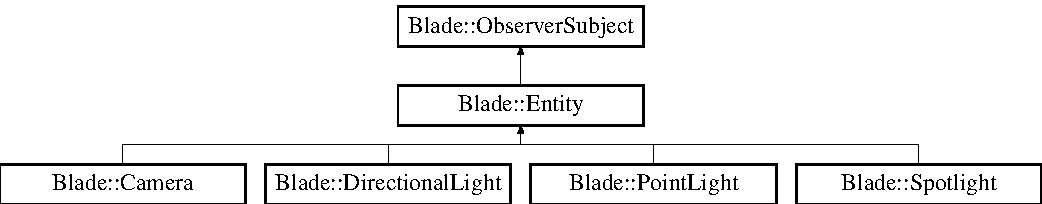
\includegraphics[height=2.727273cm]{class_blade_1_1_observer_subject}
\end{center}
\end{figure}
\subsection*{Public Member Functions}
\begin{DoxyCompactItemize}
\item 
void \hyperlink{class_blade_1_1_observer_subject_af8e103e7a7cb33062ea5fbf189902272}{Register\+Observer} (const std\+::string \&msg, \hyperlink{class_blade_1_1_observer}{Observer} $\ast$o) noexcept
\begin{DoxyCompactList}\small\item\em Register an observer for a particular type of message. \end{DoxyCompactList}\item 
void \hyperlink{class_blade_1_1_observer_subject_a780cc6b90ee1b46fe936a8c712c41a58}{Unregister\+Observer} (const std\+::string \&msg, \hyperlink{class_blade_1_1_observer}{Observer} $\ast$o) noexcept
\begin{DoxyCompactList}\small\item\em Unregister an observer for a particular type of message. \end{DoxyCompactList}\item 
void \hyperlink{class_blade_1_1_observer_subject_a4d8b26a245fa28769456e5f54049b86b}{Broadcast\+Message} (const \hyperlink{class_blade_1_1_ref_counted_container}{Message\+Container}$<$ std\+::string $>$ \&msg) const noexcept
\begin{DoxyCompactList}\small\item\em Broadcast a message to any listeners. \end{DoxyCompactList}\end{DoxyCompactItemize}


\subsection{Detailed Description}
Objeserver\+Subject implemented by the engine. 

The engine provides observer pattern interface 

\subsection{Member Function Documentation}
\mbox{\Hypertarget{class_blade_1_1_observer_subject_a4d8b26a245fa28769456e5f54049b86b}\label{class_blade_1_1_observer_subject_a4d8b26a245fa28769456e5f54049b86b}} 
\index{Blade\+::\+Observer\+Subject@{Blade\+::\+Observer\+Subject}!Broadcast\+Message@{Broadcast\+Message}}
\index{Broadcast\+Message@{Broadcast\+Message}!Blade\+::\+Observer\+Subject@{Blade\+::\+Observer\+Subject}}
\subsubsection{\texorpdfstring{Broadcast\+Message()}{BroadcastMessage()}}
{\footnotesize\ttfamily void Blade\+::\+Observer\+Subject\+::\+Broadcast\+Message (\begin{DoxyParamCaption}\item[{const \hyperlink{class_blade_1_1_ref_counted_container}{Message\+Container}$<$ std\+::string $>$ \&}]{msg }\end{DoxyParamCaption}) const\hspace{0.3cm}{\ttfamily [noexcept]}}



Broadcast a message to any listeners. 


\begin{DoxyParams}{Parameters}
{\em msg} & the message to broadcast. \\
\hline
\end{DoxyParams}
\mbox{\Hypertarget{class_blade_1_1_observer_subject_af8e103e7a7cb33062ea5fbf189902272}\label{class_blade_1_1_observer_subject_af8e103e7a7cb33062ea5fbf189902272}} 
\index{Blade\+::\+Observer\+Subject@{Blade\+::\+Observer\+Subject}!Register\+Observer@{Register\+Observer}}
\index{Register\+Observer@{Register\+Observer}!Blade\+::\+Observer\+Subject@{Blade\+::\+Observer\+Subject}}
\subsubsection{\texorpdfstring{Register\+Observer()}{RegisterObserver()}}
{\footnotesize\ttfamily void Blade\+::\+Observer\+Subject\+::\+Register\+Observer (\begin{DoxyParamCaption}\item[{const std\+::string \&}]{msg,  }\item[{\hyperlink{class_blade_1_1_observer}{Observer} $\ast$}]{o }\end{DoxyParamCaption})\hspace{0.3cm}{\ttfamily [noexcept]}}



Register an observer for a particular type of message. 


\begin{DoxyParams}{Parameters}
{\em msg} & the message type \\
\hline
{\em o} & the observer to register. \\
\hline
\end{DoxyParams}
\mbox{\Hypertarget{class_blade_1_1_observer_subject_a780cc6b90ee1b46fe936a8c712c41a58}\label{class_blade_1_1_observer_subject_a780cc6b90ee1b46fe936a8c712c41a58}} 
\index{Blade\+::\+Observer\+Subject@{Blade\+::\+Observer\+Subject}!Unregister\+Observer@{Unregister\+Observer}}
\index{Unregister\+Observer@{Unregister\+Observer}!Blade\+::\+Observer\+Subject@{Blade\+::\+Observer\+Subject}}
\subsubsection{\texorpdfstring{Unregister\+Observer()}{UnregisterObserver()}}
{\footnotesize\ttfamily void Blade\+::\+Observer\+Subject\+::\+Unregister\+Observer (\begin{DoxyParamCaption}\item[{const std\+::string \&}]{msg,  }\item[{\hyperlink{class_blade_1_1_observer}{Observer} $\ast$}]{o }\end{DoxyParamCaption})\hspace{0.3cm}{\ttfamily [noexcept]}}



Unregister an observer for a particular type of message. 


\begin{DoxyParams}{Parameters}
{\em msg} & the message type \\
\hline
{\em o} & the observer to unregister. \\
\hline
\end{DoxyParams}


The documentation for this class was generated from the following files\+:\begin{DoxyCompactItemize}
\item 
include/observer\+\_\+subject.\+h\item 
src/observer\+\_\+subject.\+cpp\end{DoxyCompactItemize}

\hypertarget{class_blade_1_1_ogg_vorbis_stream}{}\section{Blade\+:\+:Ogg\+Vorbis\+Stream Class Reference}
\label{class_blade_1_1_ogg_vorbis_stream}\index{Blade\+::\+Ogg\+Vorbis\+Stream@{Blade\+::\+Ogg\+Vorbis\+Stream}}
Inheritance diagram for Blade\+:\+:Ogg\+Vorbis\+Stream\+:\begin{figure}[H]
\begin{center}
\leavevmode
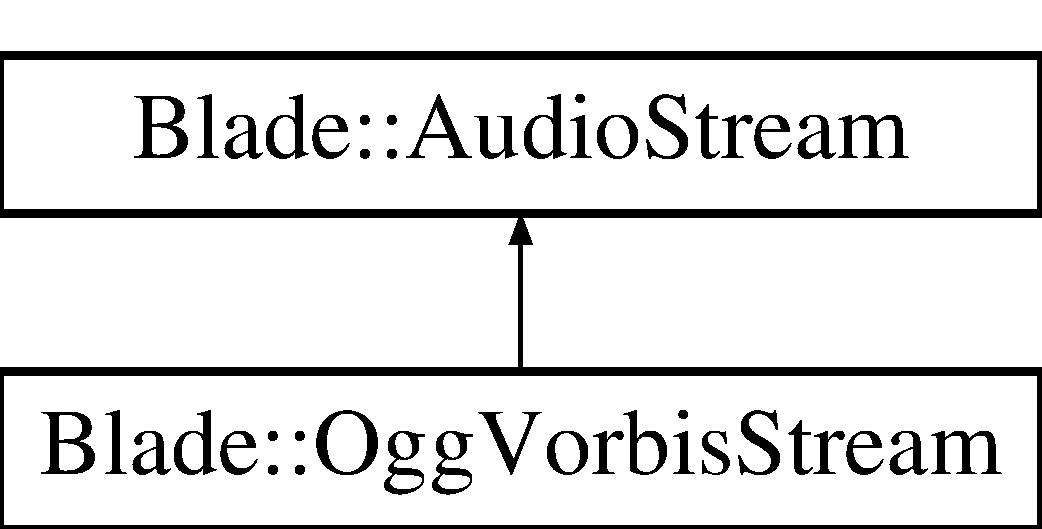
\includegraphics[height=2.000000cm]{class_blade_1_1_ogg_vorbis_stream}
\end{center}
\end{figure}
\subsection*{Public Member Functions}
\begin{DoxyCompactItemize}
\item 
\mbox{\Hypertarget{class_blade_1_1_ogg_vorbis_stream_ab6384abf34fc27973b4c48372b4d0428}\label{class_blade_1_1_ogg_vorbis_stream_ab6384abf34fc27973b4c48372b4d0428}} 
bool {\bfseries Open} (const char $\ast$fname) noexcept
\item 
\mbox{\Hypertarget{class_blade_1_1_ogg_vorbis_stream_a90a0b0dc5ee100621785c4444819cdba}\label{class_blade_1_1_ogg_vorbis_stream_a90a0b0dc5ee100621785c4444819cdba}} 
void {\bfseries Close} () noexcept
\item 
\mbox{\Hypertarget{class_blade_1_1_ogg_vorbis_stream_ac039a89c2b58d5bfd9c329b3df4e771e}\label{class_blade_1_1_ogg_vorbis_stream_ac039a89c2b58d5bfd9c329b3df4e771e}} 
void {\bfseries Play} (Audio\+Playmode mode) noexcept override
\item 
\mbox{\Hypertarget{class_blade_1_1_ogg_vorbis_stream_a2e70b39f525decae6f48efc7950e8db3}\label{class_blade_1_1_ogg_vorbis_stream_a2e70b39f525decae6f48efc7950e8db3}} 
void {\bfseries Rewind} () noexcept override
\end{DoxyCompactItemize}


The documentation for this class was generated from the following files\+:\begin{DoxyCompactItemize}
\item 
include/ovstream.\+h\item 
src/ovstream.\+cpp\end{DoxyCompactItemize}

\hypertarget{struct_blade_1_1_particle}{}\section{Blade\+:\+:Particle Struct Reference}
\label{struct_blade_1_1_particle}\index{Blade\+::\+Particle@{Blade\+::\+Particle}}
\subsection*{Public Attributes}
\begin{DoxyCompactItemize}
\item 
\mbox{\Hypertarget{struct_blade_1_1_particle_afea0f54a9dad9779c5fefdfbdc7e9eef}\label{struct_blade_1_1_particle_afea0f54a9dad9779c5fefdfbdc7e9eef}} 
Vec3f {\bfseries position}
\item 
\mbox{\Hypertarget{struct_blade_1_1_particle_a5200cd799f0aa1b9f372bef2f52b842f}\label{struct_blade_1_1_particle_a5200cd799f0aa1b9f372bef2f52b842f}} 
Vec4f {\bfseries color}
\item 
\mbox{\Hypertarget{struct_blade_1_1_particle_acf56bd264faa35cf0b355858a78944ec}\label{struct_blade_1_1_particle_acf56bd264faa35cf0b355858a78944ec}} 
float {\bfseries size}
\item 
\mbox{\Hypertarget{struct_blade_1_1_particle_a1f7ab4243f2b662167a1717255d29b16}\label{struct_blade_1_1_particle_a1f7ab4243f2b662167a1717255d29b16}} 
Vec3f {\bfseries velocity}
\item 
\mbox{\Hypertarget{struct_blade_1_1_particle_a4991a8cd32a403928d3ce0b0fed29ea1}\label{struct_blade_1_1_particle_a4991a8cd32a403928d3ce0b0fed29ea1}} 
float {\bfseries life}
\item 
\mbox{\Hypertarget{struct_blade_1_1_particle_a38ba231f0f9fe5305d2de8f9a65c4371}\label{struct_blade_1_1_particle_a38ba231f0f9fe5305d2de8f9a65c4371}} 
bool {\bfseries active}
\item 
\mbox{\Hypertarget{struct_blade_1_1_particle_af113ad28652fe7610dbd90d1c8494a75}\label{struct_blade_1_1_particle_af113ad28652fe7610dbd90d1c8494a75}} 
double {\bfseries spawn\+\_\+time}
\end{DoxyCompactItemize}


The documentation for this struct was generated from the following file\+:\begin{DoxyCompactItemize}
\item 
include/emitter\+\_\+component.\+h\end{DoxyCompactItemize}

\hypertarget{class_blade_1_1_particle_system}{}\section{Blade\+:\+:Particle\+System Class Reference}
\label{class_blade_1_1_particle_system}\index{Blade\+::\+Particle\+System@{Blade\+::\+Particle\+System}}


A system responsible of storing the Emitter\+Components.  




{\ttfamily \#include $<$particle\+\_\+system.\+h$>$}

Inheritance diagram for Blade\+:\+:Particle\+System\+:\begin{figure}[H]
\begin{center}
\leavevmode
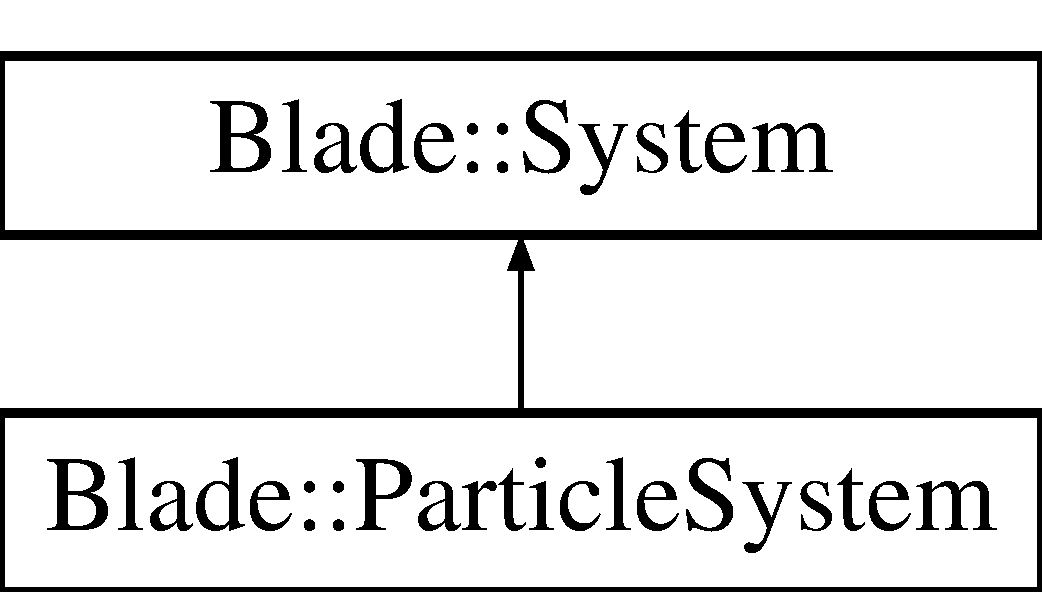
\includegraphics[height=2.000000cm]{class_blade_1_1_particle_system}
\end{center}
\end{figure}
\subsection*{Public Member Functions}
\begin{DoxyCompactItemize}
\item 
\mbox{\Hypertarget{class_blade_1_1_particle_system_a6712a38faa5ef51da4182f6a8de2487b}\label{class_blade_1_1_particle_system_a6712a38faa5ef51da4182f6a8de2487b}} 
void {\bfseries Register\+Component} (\hyperlink{class_blade_1_1_emitter_component}{Emitter\+Component} $\ast$emitter\+Component) noexcept
\item 
\mbox{\Hypertarget{class_blade_1_1_particle_system_a6a12bb122a9a34e6596faaf2e6defa11}\label{class_blade_1_1_particle_system_a6a12bb122a9a34e6596faaf2e6defa11}} 
void {\bfseries Unregister\+Component} (const int id) noexcept
\item 
bool \hyperlink{class_blade_1_1_particle_system_ae409003e325c44d82a3dcd1794ffb77d}{Initialize} () noexcept override
\begin{DoxyCompactList}\small\item\em Pure virtual method implemented by the engine\textquotesingle{}s systems to perform their initialization. \end{DoxyCompactList}\item 
\mbox{\Hypertarget{class_blade_1_1_particle_system_ae01bdc68155011d373089700cbe88f52}\label{class_blade_1_1_particle_system_ae01bdc68155011d373089700cbe88f52}} 
std\+::vector$<$ \hyperlink{class_blade_1_1_emitter_component}{Emitter\+Component} $\ast$ $>$ \& {\bfseries Get\+Emitter\+Components} () noexcept
\item 
void \hyperlink{class_blade_1_1_particle_system_a01e4983673061d797da072324a98d8d4}{Process} (float delta\+Time=.\+0f, long time=0) noexcept override
\begin{DoxyCompactList}\small\item\em Pure virtual method implemented by the engine\textquotesingle{}s systems to process the registered components. \end{DoxyCompactList}\end{DoxyCompactItemize}


\subsection{Detailed Description}
A system responsible of storing the Emitter\+Components. 

\subsection{Member Function Documentation}
\mbox{\Hypertarget{class_blade_1_1_particle_system_ae409003e325c44d82a3dcd1794ffb77d}\label{class_blade_1_1_particle_system_ae409003e325c44d82a3dcd1794ffb77d}} 
\index{Blade\+::\+Particle\+System@{Blade\+::\+Particle\+System}!Initialize@{Initialize}}
\index{Initialize@{Initialize}!Blade\+::\+Particle\+System@{Blade\+::\+Particle\+System}}
\subsubsection{\texorpdfstring{Initialize()}{Initialize()}}
{\footnotesize\ttfamily bool Blade\+::\+Particle\+System\+::\+Initialize (\begin{DoxyParamCaption}{ }\end{DoxyParamCaption})\hspace{0.3cm}{\ttfamily [override]}, {\ttfamily [virtual]}, {\ttfamily [noexcept]}}



Pure virtual method implemented by the engine\textquotesingle{}s systems to perform their initialization. 

\begin{DoxyReturn}{Returns}
T\+R\+UE if initialization is successfull, F\+A\+L\+SE otherwise. 
\end{DoxyReturn}


Implements \hyperlink{class_blade_1_1_system_a63fa00af40dc54d093300eff4785f26f}{Blade\+::\+System}.

\mbox{\Hypertarget{class_blade_1_1_particle_system_a01e4983673061d797da072324a98d8d4}\label{class_blade_1_1_particle_system_a01e4983673061d797da072324a98d8d4}} 
\index{Blade\+::\+Particle\+System@{Blade\+::\+Particle\+System}!Process@{Process}}
\index{Process@{Process}!Blade\+::\+Particle\+System@{Blade\+::\+Particle\+System}}
\subsubsection{\texorpdfstring{Process()}{Process()}}
{\footnotesize\ttfamily void Blade\+::\+Particle\+System\+::\+Process (\begin{DoxyParamCaption}\item[{float}]{delta\+Time = {\ttfamily .0f},  }\item[{long}]{time = {\ttfamily 0} }\end{DoxyParamCaption})\hspace{0.3cm}{\ttfamily [override]}, {\ttfamily [virtual]}, {\ttfamily [noexcept]}}



Pure virtual method implemented by the engine\textquotesingle{}s systems to process the registered components. 


\begin{DoxyParams}{Parameters}
{\em delta\+Time} & The time elapsed from the previous frame of the application. \\
\hline
\end{DoxyParams}


Implements \hyperlink{class_blade_1_1_system_a80c186f5f9f8fa4fd317b861853fe6a8}{Blade\+::\+System}.



The documentation for this class was generated from the following files\+:\begin{DoxyCompactItemize}
\item 
include/particle\+\_\+system.\+h\item 
src/particle\+\_\+system.\+cpp\end{DoxyCompactItemize}

\hypertarget{class_blade_1_1_pipeline}{}\section{Blade\+:\+:Pipeline$<$ T, Tdata $>$ Class Template Reference}
\label{class_blade_1_1_pipeline}\index{Blade\+::\+Pipeline$<$ T, Tdata $>$@{Blade\+::\+Pipeline$<$ T, Tdata $>$}}


Abstract class that describes a pipeline that processes the specified object data type.  




{\ttfamily \#include $<$pipeline.\+h$>$}

\subsection*{Public Member Functions}
\begin{DoxyCompactItemize}
\item 
void \hyperlink{class_blade_1_1_pipeline_a9fb99991044731f11512623dee4f1879}{Add\+Stage} (\hyperlink{class_blade_1_1_pipeline_stage}{Pipeline\+Stage}$<$ T, Tdata $>$ $\ast$stage)
\begin{DoxyCompactList}\small\item\em Adds a \hyperlink{class_blade_1_1_pipeline_stage}{Pipeline\+Stage} to the \hyperlink{class_blade_1_1_pipeline}{Pipeline}. \end{DoxyCompactList}\item 
void \hyperlink{class_blade_1_1_pipeline_a582e7f781de9f923a0c20a48019fb24f}{Execute} (const std\+::vector$<$ T $>$ \&data)
\begin{DoxyCompactList}\small\item\em Processes the objects provided by passing then through each \hyperlink{class_blade_1_1_pipeline_stage}{Pipeline\+Stage}. \end{DoxyCompactList}\end{DoxyCompactItemize}


\subsection{Detailed Description}
\subsubsection*{template$<$typename T, typename Tdata$>$\newline
class Blade\+::\+Pipeline$<$ T, Tdata $>$}

Abstract class that describes a pipeline that processes the specified object data type. 


\begin{DoxyTemplParams}{Template Parameters}
{\em T} & The type of data that the \hyperlink{class_blade_1_1_pipeline}{Pipeline}\textquotesingle{}s Pipeline\+Stages will process. \\
\hline
{\em Tdata} & The type of data that the Pipeline\+Stages will return after executed. \\
\hline
\end{DoxyTemplParams}


\subsection{Member Function Documentation}
\mbox{\Hypertarget{class_blade_1_1_pipeline_a9fb99991044731f11512623dee4f1879}\label{class_blade_1_1_pipeline_a9fb99991044731f11512623dee4f1879}} 
\index{Blade\+::\+Pipeline@{Blade\+::\+Pipeline}!Add\+Stage@{Add\+Stage}}
\index{Add\+Stage@{Add\+Stage}!Blade\+::\+Pipeline@{Blade\+::\+Pipeline}}
\subsubsection{\texorpdfstring{Add\+Stage()}{AddStage()}}
{\footnotesize\ttfamily template$<$typename T , typename Tdata $>$ \\
void \hyperlink{class_blade_1_1_pipeline}{Blade\+::\+Pipeline}$<$ T, Tdata $>$\+::Add\+Stage (\begin{DoxyParamCaption}\item[{\hyperlink{class_blade_1_1_pipeline_stage}{Pipeline\+Stage}$<$ T, Tdata $>$ $\ast$}]{stage }\end{DoxyParamCaption})\hspace{0.3cm}{\ttfamily [inline]}}



Adds a \hyperlink{class_blade_1_1_pipeline_stage}{Pipeline\+Stage} to the \hyperlink{class_blade_1_1_pipeline}{Pipeline}. 


\begin{DoxyParams}{Parameters}
{\em stage} & The \hyperlink{class_blade_1_1_pipeline_stage}{Pipeline\+Stage} to be added to the \hyperlink{class_blade_1_1_pipeline}{Pipeline}. \\
\hline
\end{DoxyParams}
\mbox{\Hypertarget{class_blade_1_1_pipeline_a582e7f781de9f923a0c20a48019fb24f}\label{class_blade_1_1_pipeline_a582e7f781de9f923a0c20a48019fb24f}} 
\index{Blade\+::\+Pipeline@{Blade\+::\+Pipeline}!Execute@{Execute}}
\index{Execute@{Execute}!Blade\+::\+Pipeline@{Blade\+::\+Pipeline}}
\subsubsection{\texorpdfstring{Execute()}{Execute()}}
{\footnotesize\ttfamily template$<$typename T , typename Tdata $>$ \\
void \hyperlink{class_blade_1_1_pipeline}{Blade\+::\+Pipeline}$<$ T, Tdata $>$\+::Execute (\begin{DoxyParamCaption}\item[{const std\+::vector$<$ T $>$ \&}]{data }\end{DoxyParamCaption})\hspace{0.3cm}{\ttfamily [inline]}}



Processes the objects provided by passing then through each \hyperlink{class_blade_1_1_pipeline_stage}{Pipeline\+Stage}. 


\begin{DoxyParams}{Parameters}
{\em data} & The objects to be processed by the \hyperlink{class_blade_1_1_pipeline}{Pipeline}\textquotesingle{}s stages. \\
\hline
\end{DoxyParams}


The documentation for this class was generated from the following file\+:\begin{DoxyCompactItemize}
\item 
include/pipeline.\+h\end{DoxyCompactItemize}

\hypertarget{class_blade_1_1_pipeline_data}{}\section{Blade\+:\+:Pipeline\+Data$<$ T $>$ Class Template Reference}
\label{class_blade_1_1_pipeline_data}\index{Blade\+::\+Pipeline\+Data$<$ T $>$@{Blade\+::\+Pipeline\+Data$<$ T $>$}}


An abstract data container for the data returned by a \hyperlink{class_blade_1_1_pipeline_stage}{Pipeline\+Stage}.  




{\ttfamily \#include $<$pipeline\+\_\+stage.\+h$>$}

\subsection*{Public Member Functions}
\begin{DoxyCompactItemize}
\item 
\hyperlink{class_blade_1_1_pipeline_data_a0ec5d639a520d7c39593d62084788398}{Pipeline\+Data} (T data)
\begin{DoxyCompactList}\small\item\em \hyperlink{class_blade_1_1_pipeline_data}{Pipeline\+Data} constructor. \end{DoxyCompactList}\item 
T \hyperlink{class_blade_1_1_pipeline_data_a5fabd7938e03537063559256d21c8253}{Get} () const noexcept
\begin{DoxyCompactList}\small\item\em Returns the data contained in the \hyperlink{class_blade_1_1_pipeline_data}{Pipeline\+Data} container. \end{DoxyCompactList}\end{DoxyCompactItemize}


\subsection{Detailed Description}
\subsubsection*{template$<$typename T$>$\newline
class Blade\+::\+Pipeline\+Data$<$ T $>$}

An abstract data container for the data returned by a \hyperlink{class_blade_1_1_pipeline_stage}{Pipeline\+Stage}. 


\begin{DoxyTemplParams}{Template Parameters}
{\em T} & The type of data the container will hold. \\
\hline
\end{DoxyTemplParams}


\subsection{Constructor \& Destructor Documentation}
\mbox{\Hypertarget{class_blade_1_1_pipeline_data_a0ec5d639a520d7c39593d62084788398}\label{class_blade_1_1_pipeline_data_a0ec5d639a520d7c39593d62084788398}} 
\index{Blade\+::\+Pipeline\+Data@{Blade\+::\+Pipeline\+Data}!Pipeline\+Data@{Pipeline\+Data}}
\index{Pipeline\+Data@{Pipeline\+Data}!Blade\+::\+Pipeline\+Data@{Blade\+::\+Pipeline\+Data}}
\subsubsection{\texorpdfstring{Pipeline\+Data()}{PipelineData()}}
{\footnotesize\ttfamily template$<$typename T$>$ \\
\hyperlink{class_blade_1_1_pipeline_data}{Blade\+::\+Pipeline\+Data}$<$ T $>$\+::\hyperlink{class_blade_1_1_pipeline_data}{Pipeline\+Data} (\begin{DoxyParamCaption}\item[{T}]{data }\end{DoxyParamCaption})\hspace{0.3cm}{\ttfamily [inline]}, {\ttfamily [explicit]}}



\hyperlink{class_blade_1_1_pipeline_data}{Pipeline\+Data} constructor. 


\begin{DoxyParams}{Parameters}
{\em data} & The data to store in the container. \\
\hline
\end{DoxyParams}


\subsection{Member Function Documentation}
\mbox{\Hypertarget{class_blade_1_1_pipeline_data_a5fabd7938e03537063559256d21c8253}\label{class_blade_1_1_pipeline_data_a5fabd7938e03537063559256d21c8253}} 
\index{Blade\+::\+Pipeline\+Data@{Blade\+::\+Pipeline\+Data}!Get@{Get}}
\index{Get@{Get}!Blade\+::\+Pipeline\+Data@{Blade\+::\+Pipeline\+Data}}
\subsubsection{\texorpdfstring{Get()}{Get()}}
{\footnotesize\ttfamily template$<$typename T$>$ \\
T \hyperlink{class_blade_1_1_pipeline_data}{Blade\+::\+Pipeline\+Data}$<$ T $>$\+::Get (\begin{DoxyParamCaption}{ }\end{DoxyParamCaption}) const\hspace{0.3cm}{\ttfamily [inline]}, {\ttfamily [noexcept]}}



Returns the data contained in the \hyperlink{class_blade_1_1_pipeline_data}{Pipeline\+Data} container. 

\begin{DoxyReturn}{Returns}
The data contained in the container. 
\end{DoxyReturn}


The documentation for this class was generated from the following file\+:\begin{DoxyCompactItemize}
\item 
include/pipeline\+\_\+stage.\+h\end{DoxyCompactItemize}

\hypertarget{class_blade_1_1_pipeline_stage}{}\section{Blade\+:\+:Pipeline\+Stage$<$ T, Tdata $>$ Class Template Reference}
\label{class_blade_1_1_pipeline_stage}\index{Blade\+::\+Pipeline\+Stage$<$ T, Tdata $>$@{Blade\+::\+Pipeline\+Stage$<$ T, Tdata $>$}}


This class describes an abstract stage of a pipeline that processes the specified type of data and returns the specified type of data.  




{\ttfamily \#include $<$pipeline\+\_\+stage.\+h$>$}

\subsection*{Public Member Functions}
\begin{DoxyCompactItemize}
\item 
\hyperlink{class_blade_1_1_pipeline_stage_acc9f2dc27495c661bd4d985f9b7ab764}{Pipeline\+Stage} (const std\+::string \&name)
\begin{DoxyCompactList}\small\item\em \hyperlink{class_blade_1_1_pipeline_stage}{Pipeline\+Stage} constructor. \end{DoxyCompactList}\item 
\mbox{\Hypertarget{class_blade_1_1_pipeline_stage_a305d6399b99d4bc67ebd6512eedead8a}\label{class_blade_1_1_pipeline_stage_a305d6399b99d4bc67ebd6512eedead8a}} 
virtual \hyperlink{class_blade_1_1_pipeline_stage_a305d6399b99d4bc67ebd6512eedead8a}{$\sim$\+Pipeline\+Stage} ()=default
\begin{DoxyCompactList}\small\item\em Default destructor of the \hyperlink{class_blade_1_1_pipeline_stage}{Pipeline\+Stage}. \end{DoxyCompactList}\item 
virtual bool \hyperlink{class_blade_1_1_pipeline_stage_a0b1cca63a255807448e12721c60d91fc}{Initialize} ()=0
\begin{DoxyCompactList}\small\item\em Initializes the \hyperlink{class_blade_1_1_pipeline_stage}{Pipeline\+Stage}. \end{DoxyCompactList}\item 
virtual \hyperlink{class_blade_1_1_pipeline_data}{Pipeline\+Data}$<$ Tdata $>$ \hyperlink{class_blade_1_1_pipeline_stage_a0536c99a8bfd4dc16c6b5d7dca43ed58}{Execute} (const std\+::vector$<$ T $>$ \&data, const \hyperlink{class_blade_1_1_pipeline_data}{Pipeline\+Data}$<$ Tdata $>$ \&tdata) noexcept=0
\begin{DoxyCompactList}\small\item\em Processes the vector of objects provided and return the result. \end{DoxyCompactList}\end{DoxyCompactItemize}


\subsection{Detailed Description}
\subsubsection*{template$<$typename T, typename Tdata$>$\newline
class Blade\+::\+Pipeline\+Stage$<$ T, Tdata $>$}

This class describes an abstract stage of a pipeline that processes the specified type of data and returns the specified type of data. 


\begin{DoxyTemplParams}{Template Parameters}
{\em T} & The type of data the \hyperlink{class_blade_1_1_pipeline_stage}{Pipeline\+Stage} will process. \\
\hline
{\em Tdata} & The type of data the \hyperlink{class_blade_1_1_pipeline_stage}{Pipeline\+Stage} will return. \\
\hline
\end{DoxyTemplParams}


\subsection{Constructor \& Destructor Documentation}
\mbox{\Hypertarget{class_blade_1_1_pipeline_stage_acc9f2dc27495c661bd4d985f9b7ab764}\label{class_blade_1_1_pipeline_stage_acc9f2dc27495c661bd4d985f9b7ab764}} 
\index{Blade\+::\+Pipeline\+Stage@{Blade\+::\+Pipeline\+Stage}!Pipeline\+Stage@{Pipeline\+Stage}}
\index{Pipeline\+Stage@{Pipeline\+Stage}!Blade\+::\+Pipeline\+Stage@{Blade\+::\+Pipeline\+Stage}}
\subsubsection{\texorpdfstring{Pipeline\+Stage()}{PipelineStage()}}
{\footnotesize\ttfamily template$<$typename T, typename Tdata$>$ \\
\hyperlink{class_blade_1_1_pipeline_stage}{Blade\+::\+Pipeline\+Stage}$<$ T, Tdata $>$\+::\hyperlink{class_blade_1_1_pipeline_stage}{Pipeline\+Stage} (\begin{DoxyParamCaption}\item[{const std\+::string \&}]{name }\end{DoxyParamCaption})\hspace{0.3cm}{\ttfamily [inline]}, {\ttfamily [explicit]}}



\hyperlink{class_blade_1_1_pipeline_stage}{Pipeline\+Stage} constructor. 


\begin{DoxyParams}{Parameters}
{\em name} & The name of the \hyperlink{class_blade_1_1_pipeline_stage}{Pipeline\+Stage}. \\
\hline
\end{DoxyParams}


\subsection{Member Function Documentation}
\mbox{\Hypertarget{class_blade_1_1_pipeline_stage_a0536c99a8bfd4dc16c6b5d7dca43ed58}\label{class_blade_1_1_pipeline_stage_a0536c99a8bfd4dc16c6b5d7dca43ed58}} 
\index{Blade\+::\+Pipeline\+Stage@{Blade\+::\+Pipeline\+Stage}!Execute@{Execute}}
\index{Execute@{Execute}!Blade\+::\+Pipeline\+Stage@{Blade\+::\+Pipeline\+Stage}}
\subsubsection{\texorpdfstring{Execute()}{Execute()}}
{\footnotesize\ttfamily template$<$typename T, typename Tdata$>$ \\
virtual \hyperlink{class_blade_1_1_pipeline_data}{Pipeline\+Data}$<$Tdata$>$ \hyperlink{class_blade_1_1_pipeline_stage}{Blade\+::\+Pipeline\+Stage}$<$ T, Tdata $>$\+::Execute (\begin{DoxyParamCaption}\item[{const std\+::vector$<$ T $>$ \&}]{data,  }\item[{const \hyperlink{class_blade_1_1_pipeline_data}{Pipeline\+Data}$<$ Tdata $>$ \&}]{tdata }\end{DoxyParamCaption})\hspace{0.3cm}{\ttfamily [pure virtual]}, {\ttfamily [noexcept]}}



Processes the vector of objects provided and return the result. 


\begin{DoxyParams}{Parameters}
{\em data} & The type of data the \hyperlink{class_blade_1_1_pipeline_stage}{Pipeline\+Stage} will process. \\
\hline
{\em tdata} & The type of data the \hyperlink{class_blade_1_1_pipeline_stage}{Pipeline\+Stage} will return. \\
\hline
\end{DoxyParams}
\begin{DoxyReturn}{Returns}
A \hyperlink{class_blade_1_1_pipeline_data}{Pipeline\+Data} container with the the appropriate data type encapsulated. 
\end{DoxyReturn}
\mbox{\Hypertarget{class_blade_1_1_pipeline_stage_a0b1cca63a255807448e12721c60d91fc}\label{class_blade_1_1_pipeline_stage_a0b1cca63a255807448e12721c60d91fc}} 
\index{Blade\+::\+Pipeline\+Stage@{Blade\+::\+Pipeline\+Stage}!Initialize@{Initialize}}
\index{Initialize@{Initialize}!Blade\+::\+Pipeline\+Stage@{Blade\+::\+Pipeline\+Stage}}
\subsubsection{\texorpdfstring{Initialize()}{Initialize()}}
{\footnotesize\ttfamily template$<$typename T, typename Tdata$>$ \\
virtual bool \hyperlink{class_blade_1_1_pipeline_stage}{Blade\+::\+Pipeline\+Stage}$<$ T, Tdata $>$\+::Initialize (\begin{DoxyParamCaption}{ }\end{DoxyParamCaption})\hspace{0.3cm}{\ttfamily [pure virtual]}}



Initializes the \hyperlink{class_blade_1_1_pipeline_stage}{Pipeline\+Stage}. 

\begin{DoxyReturn}{Returns}
T\+R\+UE if initialization succeded, F\+A\+L\+SE otherwise. 
\end{DoxyReturn}


The documentation for this class was generated from the following file\+:\begin{DoxyCompactItemize}
\item 
include/pipeline\+\_\+stage.\+h\end{DoxyCompactItemize}

\hypertarget{class_blade_1_1_plane_collider}{}\section{Blade\+:\+:Plane\+Collider Class Reference}
\label{class_blade_1_1_plane_collider}\index{Blade\+::\+Plane\+Collider@{Blade\+::\+Plane\+Collider}}


Bounding Plane class is a collider.  




{\ttfamily \#include $<$plane\+\_\+collider.\+h$>$}

Inheritance diagram for Blade\+:\+:Plane\+Collider\+:\begin{figure}[H]
\begin{center}
\leavevmode
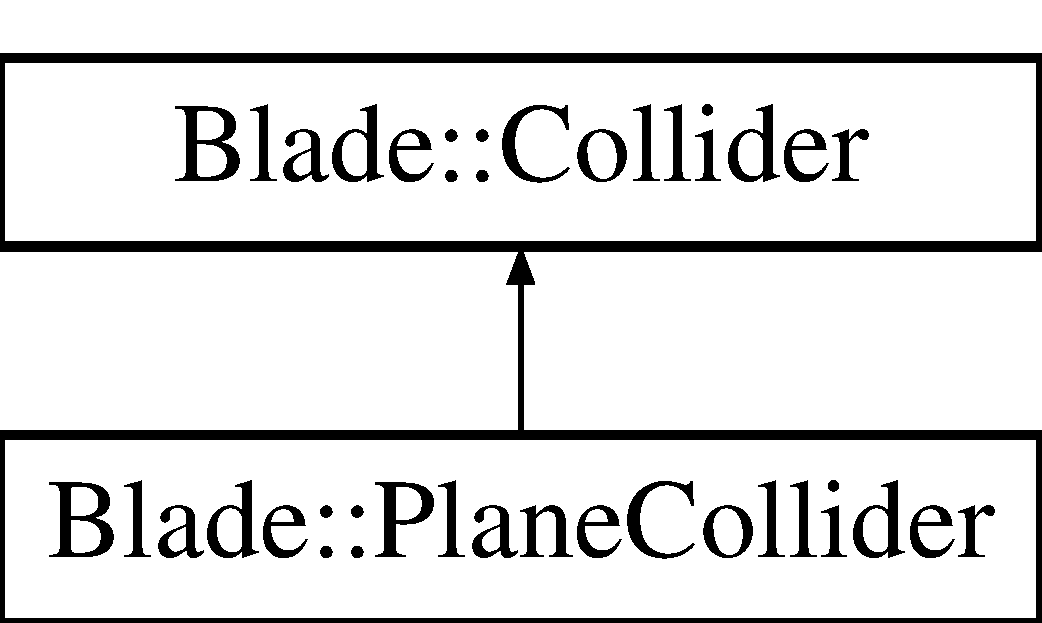
\includegraphics[height=2.000000cm]{class_blade_1_1_plane_collider}
\end{center}
\end{figure}
\subsection*{Public Member Functions}
\begin{DoxyCompactItemize}
\item 
\mbox{\Hypertarget{class_blade_1_1_plane_collider_afde68d33241cd30bc0a68c29ba5ab177}\label{class_blade_1_1_plane_collider_afde68d33241cd30bc0a68c29ba5ab177}} 
{\bfseries Plane\+Collider} (const Vec3f \&plane\+Normal, const float offset)
\item 
\mbox{\Hypertarget{class_blade_1_1_plane_collider_a0eec57eec3a14a57ddbb14549e3f4de8}\label{class_blade_1_1_plane_collider_a0eec57eec3a14a57ddbb14549e3f4de8}} 
bool {\bfseries Collide} (const \hyperlink{class_blade_1_1_collider}{Collider} $\ast$collider, \hyperlink{class_blade_1_1_contact_manifold}{Contact\+Manifold} \&manifold) const noexcept override
\item 
\mbox{\Hypertarget{class_blade_1_1_plane_collider_a41656313053cd2529b0815deb94d2713}\label{class_blade_1_1_plane_collider_a41656313053cd2529b0815deb94d2713}} 
bool {\bfseries Collide} (const \hyperlink{class_blade_1_1_bounding_sphere}{Bounding\+Sphere} $\ast$bsphere, \hyperlink{class_blade_1_1_contact_manifold}{Contact\+Manifold} \&manifold) const noexcept override
\item 
\mbox{\Hypertarget{class_blade_1_1_plane_collider_a06dbb0b93993c13c36b9fcfcdfa2a19b}\label{class_blade_1_1_plane_collider_a06dbb0b93993c13c36b9fcfcdfa2a19b}} 
bool {\bfseries Collide} (const \hyperlink{class_blade_1_1_plane_collider}{Plane\+Collider} $\ast$plane, \hyperlink{class_blade_1_1_contact_manifold}{Contact\+Manifold} \&manifold) const noexcept override
\item 
\mbox{\Hypertarget{class_blade_1_1_plane_collider_a34f5aed7ac8bf8fde0d7e4b2981d6468}\label{class_blade_1_1_plane_collider_a34f5aed7ac8bf8fde0d7e4b2981d6468}} 
const Vec3f \& {\bfseries Get\+Plane\+Normal} () const noexcept
\item 
\mbox{\Hypertarget{class_blade_1_1_plane_collider_a7c958fc80ebb794cbe9b321335ab1a7c}\label{class_blade_1_1_plane_collider_a7c958fc80ebb794cbe9b321335ab1a7c}} 
void {\bfseries Set\+Plane\+Normal} (const Vec3f \&normal) noexcept
\item 
\mbox{\Hypertarget{class_blade_1_1_plane_collider_aa139681f2b510ca30dd86e0c9e22d919}\label{class_blade_1_1_plane_collider_aa139681f2b510ca30dd86e0c9e22d919}} 
float {\bfseries Get\+Offeset} () const noexcept
\item 
\mbox{\Hypertarget{class_blade_1_1_plane_collider_a858ff3ff302c656cf1d0b0387802588d}\label{class_blade_1_1_plane_collider_a858ff3ff302c656cf1d0b0387802588d}} 
void {\bfseries Set\+Offset} (const float offset) noexcept
\end{DoxyCompactItemize}


\subsection{Detailed Description}
Bounding Plane class is a collider. 

The documentation for this class was generated from the following files\+:\begin{DoxyCompactItemize}
\item 
include/plane\+\_\+collider.\+h\item 
src/plane\+\_\+collider.\+cpp\end{DoxyCompactItemize}

\hypertarget{class_blade_1_1_point_light}{}\section{Blade\+:\+:Point\+Light Class Reference}
\label{class_blade_1_1_point_light}\index{Blade\+::\+Point\+Light@{Blade\+::\+Point\+Light}}
Inheritance diagram for Blade\+:\+:Point\+Light\+:\begin{figure}[H]
\begin{center}
\leavevmode
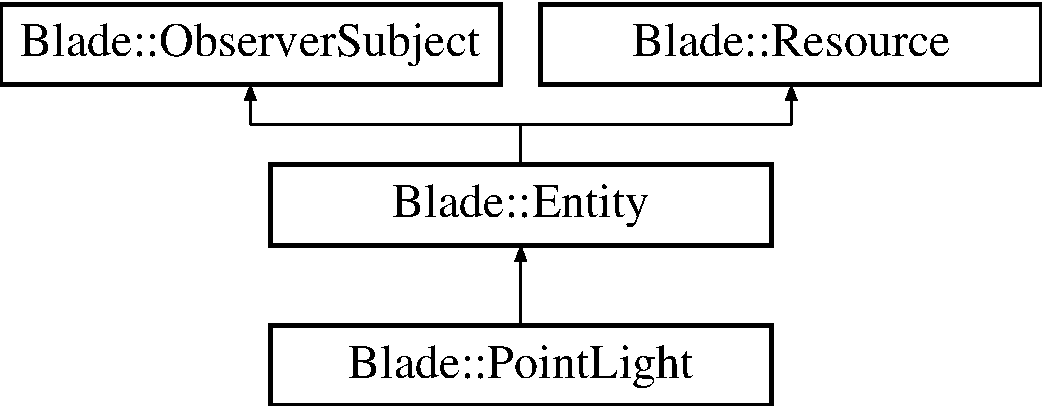
\includegraphics[height=3.000000cm]{class_blade_1_1_point_light}
\end{center}
\end{figure}
\subsection*{Public Member Functions}
\begin{DoxyCompactItemize}
\item 
\mbox{\Hypertarget{class_blade_1_1_point_light_a4b51a3939ac5b592075f6feb88a78366}\label{class_blade_1_1_point_light_a4b51a3939ac5b592075f6feb88a78366}} 
{\bfseries Point\+Light} (const std\+::string \&name, const \hyperlink{struct_blade_1_1_point_light_desc}{Point\+Light\+Desc} \&light\+Description)
\end{DoxyCompactItemize}


The documentation for this class was generated from the following files\+:\begin{DoxyCompactItemize}
\item 
include/point\+\_\+light.\+h\item 
src/point\+\_\+light.\+cpp\end{DoxyCompactItemize}

\hypertarget{class_blade_1_1_point_light_component}{}\section{Blade\+:\+:Point\+Light\+Component Class Reference}
\label{class_blade_1_1_point_light_component}\index{Blade\+::\+Point\+Light\+Component@{Blade\+::\+Point\+Light\+Component}}
Inheritance diagram for Blade\+:\+:Point\+Light\+Component\+:\begin{figure}[H]
\begin{center}
\leavevmode
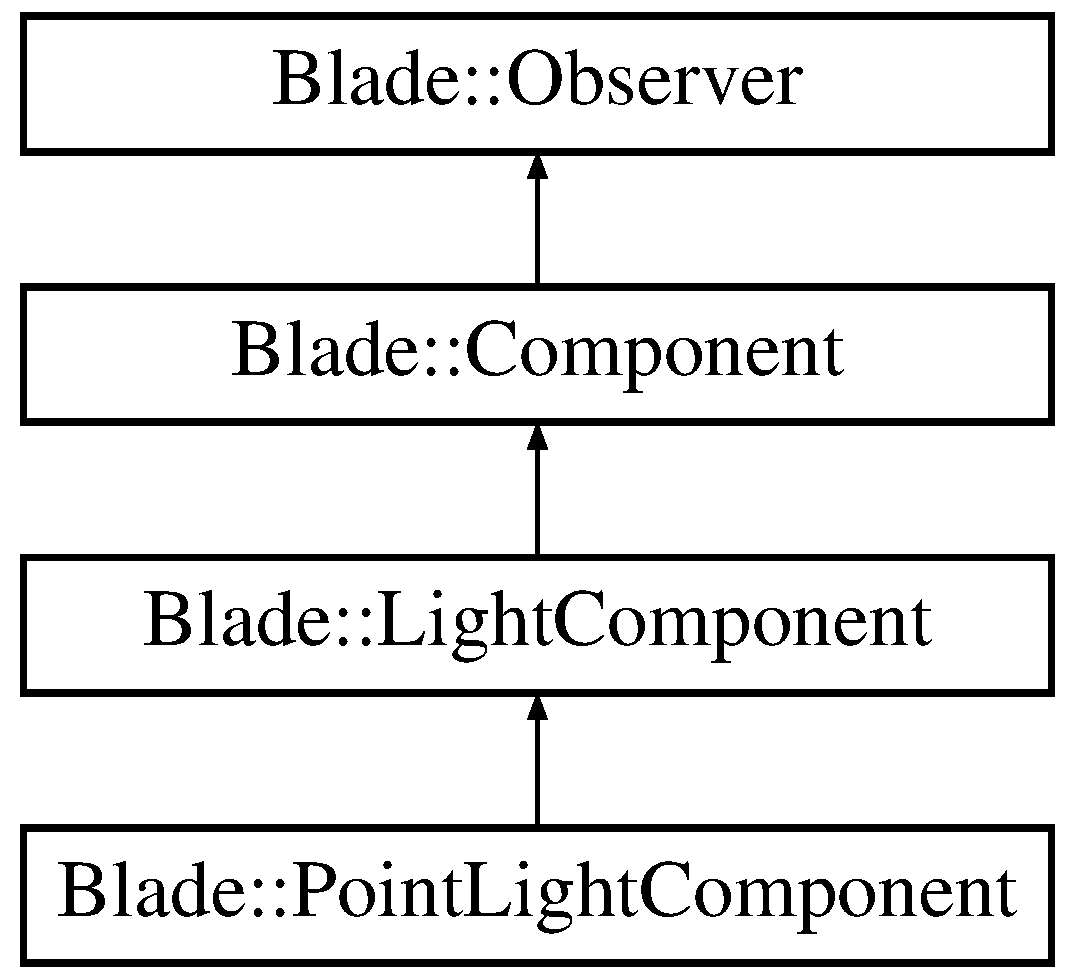
\includegraphics[height=4.000000cm]{class_blade_1_1_point_light_component}
\end{center}
\end{figure}
\subsection*{Public Member Functions}
\begin{DoxyCompactItemize}
\item 
\mbox{\Hypertarget{class_blade_1_1_point_light_component_afc983955082f9842299378143cc41498}\label{class_blade_1_1_point_light_component_afc983955082f9842299378143cc41498}} 
{\bfseries Point\+Light\+Component} (const \hyperlink{struct_blade_1_1_point_light_desc}{Point\+Light\+Desc} \&light\+Desc, \hyperlink{class_blade_1_1_entity}{Entity} $\ast$parent)
\item 
\mbox{\Hypertarget{class_blade_1_1_point_light_component_ab3c163157873a1561f5f8f7b7dd377e5}\label{class_blade_1_1_point_light_component_ab3c163157873a1561f5f8f7b7dd377e5}} 
const \hyperlink{struct_blade_1_1_point_light_desc}{Point\+Light\+Desc} \& {\bfseries Get\+Light\+Description} () const noexcept
\item 
\mbox{\Hypertarget{class_blade_1_1_point_light_component_acdfbc0b246f0b93cdb686105a2f2b46f}\label{class_blade_1_1_point_light_component_acdfbc0b246f0b93cdb686105a2f2b46f}} 
\hyperlink{struct_blade_1_1_point_light_desc}{Point\+Light\+Desc} $\ast$ {\bfseries Get\+Light\+Description\+Ptr} () noexcept
\end{DoxyCompactItemize}


The documentation for this class was generated from the following files\+:\begin{DoxyCompactItemize}
\item 
include/point\+\_\+light\+\_\+component.\+h\item 
src/point\+\_\+light\+\_\+component.\+cpp\end{DoxyCompactItemize}

\hypertarget{struct_blade_1_1_point_light_desc}{}\section{Blade\+:\+:Point\+Light\+Desc Struct Reference}
\label{struct_blade_1_1_point_light_desc}\index{Blade\+::\+Point\+Light\+Desc@{Blade\+::\+Point\+Light\+Desc}}


A struct describing a point light.  




{\ttfamily \#include $<$light\+\_\+component.\+h$>$}

\subsection*{Public Attributes}
\begin{DoxyCompactItemize}
\item 
\mbox{\Hypertarget{struct_blade_1_1_point_light_desc_ab5a5c5594188eb4a48433a57c69e223c}\label{struct_blade_1_1_point_light_desc_ab5a5c5594188eb4a48433a57c69e223c}} 
Vec4f {\bfseries ambient\+Intensity}
\item 
\mbox{\Hypertarget{struct_blade_1_1_point_light_desc_a5da1931cba52459b067e689fa9347963}\label{struct_blade_1_1_point_light_desc_a5da1931cba52459b067e689fa9347963}} 
Vec4f {\bfseries diffuse\+Intensity}
\item 
\mbox{\Hypertarget{struct_blade_1_1_point_light_desc_adcead88e629c1e9defba3aee8085a1e2}\label{struct_blade_1_1_point_light_desc_adcead88e629c1e9defba3aee8085a1e2}} 
Vec4f {\bfseries specular\+Intensity}
\item 
\mbox{\Hypertarget{struct_blade_1_1_point_light_desc_a4a566f59cabe3382fb278957a411952b}\label{struct_blade_1_1_point_light_desc_a4a566f59cabe3382fb278957a411952b}} 
Vec3f {\bfseries position}
\item 
\mbox{\Hypertarget{struct_blade_1_1_point_light_desc_a5693572f09d64d19554c7cbceac7f4ec}\label{struct_blade_1_1_point_light_desc_a5693572f09d64d19554c7cbceac7f4ec}} 
float {\bfseries constant\+Attenuation}
\item 
\mbox{\Hypertarget{struct_blade_1_1_point_light_desc_a4bef661df60949afcdc00bf4b29f7c0e}\label{struct_blade_1_1_point_light_desc_a4bef661df60949afcdc00bf4b29f7c0e}} 
float {\bfseries linear\+Attenuation}
\item 
\mbox{\Hypertarget{struct_blade_1_1_point_light_desc_a9ec597895c5523456a17247a7aac4487}\label{struct_blade_1_1_point_light_desc_a9ec597895c5523456a17247a7aac4487}} 
float {\bfseries quadratic\+Attenuation}
\item 
\mbox{\Hypertarget{struct_blade_1_1_point_light_desc_abe2d8b440bc43e88702140a1a45e0888}\label{struct_blade_1_1_point_light_desc_abe2d8b440bc43e88702140a1a45e0888}} 
Vec2f {\bfseries pad}
\end{DoxyCompactItemize}


\subsection{Detailed Description}
A struct describing a point light. 

This struct is also used to represent a point light in shaders. 

The documentation for this struct was generated from the following file\+:\begin{DoxyCompactItemize}
\item 
include/light\+\_\+component.\+h\end{DoxyCompactItemize}

\hypertarget{class_blade_1_1_ref_counted_container}{}\section{Blade\+:\+:Ref\+Counted\+Container$<$ T $>$ Class Template Reference}
\label{class_blade_1_1_ref_counted_container}\index{Blade\+::\+Ref\+Counted\+Container$<$ T $>$@{Blade\+::\+Ref\+Counted\+Container$<$ T $>$}}
\subsection*{Public Member Functions}
\begin{DoxyCompactItemize}
\item 
\mbox{\Hypertarget{class_blade_1_1_ref_counted_container_a0fb18560e2c5e73fc8f26d0df78cb696}\label{class_blade_1_1_ref_counted_container_a0fb18560e2c5e73fc8f26d0df78cb696}} 
{\bfseries Ref\+Counted\+Container} (T $\ast$item)
\item 
\mbox{\Hypertarget{class_blade_1_1_ref_counted_container_a3ad6ba693cc2c0fa7a50b4acd7fba8a1}\label{class_blade_1_1_ref_counted_container_a3ad6ba693cc2c0fa7a50b4acd7fba8a1}} 
{\bfseries Ref\+Counted\+Container} (const \hyperlink{class_blade_1_1_ref_counted_container}{Ref\+Counted\+Container} \&other)
\item 
\mbox{\Hypertarget{class_blade_1_1_ref_counted_container_ac9d85744784db9cfbe196cbd6abfd8d2}\label{class_blade_1_1_ref_counted_container_ac9d85744784db9cfbe196cbd6abfd8d2}} 
{\bfseries Ref\+Counted\+Container} (\hyperlink{class_blade_1_1_ref_counted_container}{Ref\+Counted\+Container} \&\&other) noexcept=delete
\item 
\mbox{\Hypertarget{class_blade_1_1_ref_counted_container_acf5a91f226347ee889ba699c254c71c3}\label{class_blade_1_1_ref_counted_container_acf5a91f226347ee889ba699c254c71c3}} 
\hyperlink{class_blade_1_1_ref_counted_container}{Ref\+Counted\+Container} \& {\bfseries operator=} (const \hyperlink{class_blade_1_1_ref_counted_container}{Ref\+Counted\+Container} \&other)
\item 
\mbox{\Hypertarget{class_blade_1_1_ref_counted_container_ae3e44758f8646176904f38c71266791f}\label{class_blade_1_1_ref_counted_container_ae3e44758f8646176904f38c71266791f}} 
\hyperlink{class_blade_1_1_ref_counted_container}{Ref\+Counted\+Container} \& {\bfseries operator=} (\hyperlink{class_blade_1_1_ref_counted_container}{Ref\+Counted\+Container} \&\&other) noexcept=delete
\item 
\mbox{\Hypertarget{class_blade_1_1_ref_counted_container_a903d52fa217c9e6e30d931f5a9703c61}\label{class_blade_1_1_ref_counted_container_a903d52fa217c9e6e30d931f5a9703c61}} 
void {\bfseries Add\+Reference} () noexcept
\item 
\mbox{\Hypertarget{class_blade_1_1_ref_counted_container_aa356873bea32f885d723bc93ae559880}\label{class_blade_1_1_ref_counted_container_aa356873bea32f885d723bc93ae559880}} 
void {\bfseries Subtract\+Reference} () noexcept
\item 
\mbox{\Hypertarget{class_blade_1_1_ref_counted_container_a4353b01bfcfd39df50c7d8a6f68d73ec}\label{class_blade_1_1_ref_counted_container_a4353b01bfcfd39df50c7d8a6f68d73ec}} 
int {\bfseries Get\+Reference\+Count} () const noexcept
\item 
\mbox{\Hypertarget{class_blade_1_1_ref_counted_container_aea9ac6e25ecc0775a9f91145958b6f2d}\label{class_blade_1_1_ref_counted_container_aea9ac6e25ecc0775a9f91145958b6f2d}} 
T $\ast$ {\bfseries Get} () const noexcept
\end{DoxyCompactItemize}


The documentation for this class was generated from the following file\+:\begin{DoxyCompactItemize}
\item 
include/ref\+\_\+counted\+\_\+container.\+h\end{DoxyCompactItemize}

\hypertarget{class_blade_1_1_render_component}{}\section{Blade\+:\+:Render\+Component Class Reference}
\label{class_blade_1_1_render_component}\index{Blade\+::\+Render\+Component@{Blade\+::\+Render\+Component}}


Represents a \hyperlink{class_blade_1_1_render_component}{Render\+Component}. The \hyperlink{class_blade_1_1_render_component}{Render\+Component} makes an entity renderable. This component is processed by the \hyperlink{class_blade_1_1_render_system}{Render\+System}.  




{\ttfamily \#include $<$render\+\_\+component.\+h$>$}

Inheritance diagram for Blade\+:\+:Render\+Component\+:\begin{figure}[H]
\begin{center}
\leavevmode
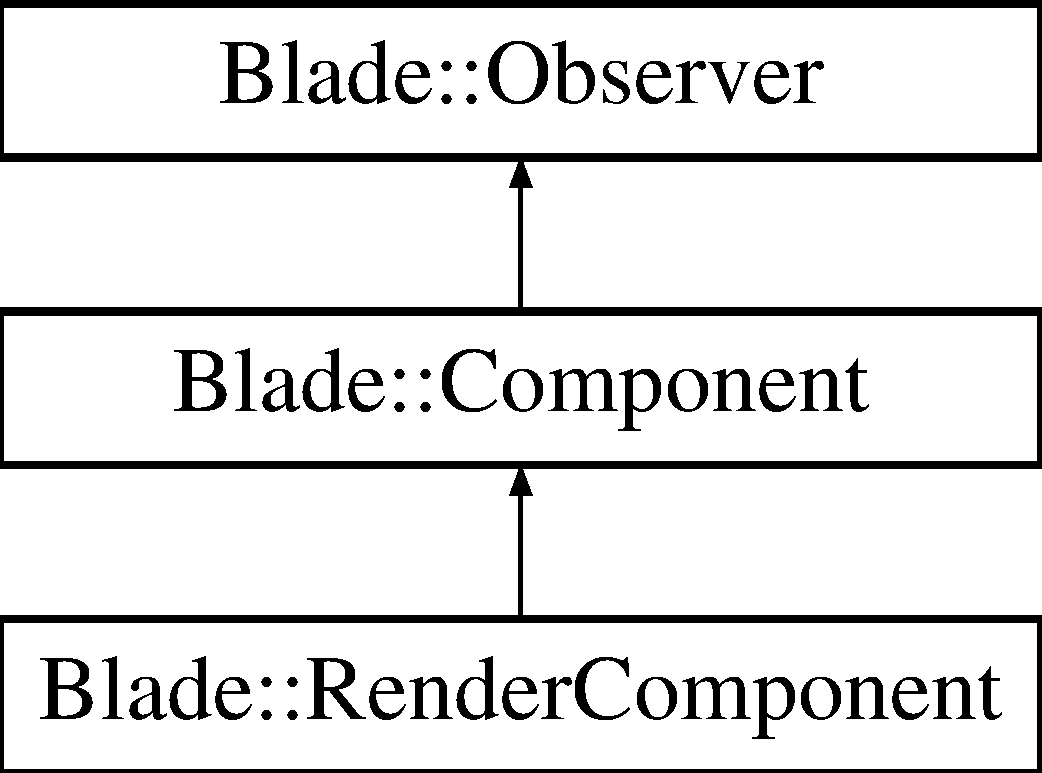
\includegraphics[height=3.000000cm]{class_blade_1_1_render_component}
\end{center}
\end{figure}
\subsection*{Public Member Functions}
\begin{DoxyCompactItemize}
\item 
\hyperlink{class_blade_1_1_render_component_a7bd09f012ebce3b94c882ed4afd5698f}{Render\+Component} (\hyperlink{class_blade_1_1_entity}{Entity} $\ast$parent)
\begin{DoxyCompactList}\small\item\em \hyperlink{class_blade_1_1_render_component}{Render\+Component}\textquotesingle{}s constructor. Registers the \hyperlink{class_blade_1_1_render_component}{Render\+Component} to the \hyperlink{class_blade_1_1_render_system}{Render\+System}. \end{DoxyCompactList}\item 
\mbox{\Hypertarget{class_blade_1_1_render_component_ac187f8f4f63a009a15abc6ebfba85b10}\label{class_blade_1_1_render_component_ac187f8f4f63a009a15abc6ebfba85b10}} 
\hyperlink{class_blade_1_1_render_component_ac187f8f4f63a009a15abc6ebfba85b10}{$\sim$\+Render\+Component} ()
\begin{DoxyCompactList}\small\item\em \hyperlink{class_blade_1_1_render_component}{Render\+Component}\textquotesingle{}s destructor. Unregisters the \hyperlink{class_blade_1_1_render_component}{Render\+Component} from the \hyperlink{class_blade_1_1_render_system}{Render\+System}. \end{DoxyCompactList}\item 
\hyperlink{class_blade_1_1_mesh}{Mesh} $\ast$ \hyperlink{class_blade_1_1_render_component_acd44eb4419c5c412fbaf080b039b3f44}{Get\+Mesh} () const noexcept
\begin{DoxyCompactList}\small\item\em Provides a pointer to the \hyperlink{class_blade_1_1_mesh}{Mesh} contained in the \hyperlink{class_blade_1_1_render_component}{Render\+Component}. \end{DoxyCompactList}\item 
void \hyperlink{class_blade_1_1_render_component_a23d49cb161e26089cc246c9fb5f739a8}{Set\+Mesh} (\hyperlink{class_blade_1_1_mesh}{Mesh} $\ast$mesh) noexcept
\begin{DoxyCompactList}\small\item\em Sets the specified \hyperlink{class_blade_1_1_mesh}{Mesh} to the \hyperlink{class_blade_1_1_render_component}{Render\+Component}. \end{DoxyCompactList}\item 
const \hyperlink{struct_blade_1_1_material}{Material} \& \hyperlink{class_blade_1_1_render_component_a8d8d98cd4f9e559160fcb9ebcaf07fbb}{Get\+Material} () const noexcept
\begin{DoxyCompactList}\small\item\em Provides the \hyperlink{struct_blade_1_1_material}{Material} of the \hyperlink{class_blade_1_1_render_component}{Render\+Component}. \end{DoxyCompactList}\item 
void \hyperlink{class_blade_1_1_render_component_ae985d0c5ac2ff9eb158683e72203ddf1}{Set\+Material} (const \hyperlink{struct_blade_1_1_material}{Material} \&material) noexcept
\begin{DoxyCompactList}\small\item\em Sets the specified \hyperlink{struct_blade_1_1_material}{Material} to the \hyperlink{class_blade_1_1_render_component}{Render\+Component}. \end{DoxyCompactList}\end{DoxyCompactItemize}


\subsection{Detailed Description}
Represents a \hyperlink{class_blade_1_1_render_component}{Render\+Component}. The \hyperlink{class_blade_1_1_render_component}{Render\+Component} makes an entity renderable. This component is processed by the \hyperlink{class_blade_1_1_render_system}{Render\+System}. 

\subsection{Constructor \& Destructor Documentation}
\mbox{\Hypertarget{class_blade_1_1_render_component_a7bd09f012ebce3b94c882ed4afd5698f}\label{class_blade_1_1_render_component_a7bd09f012ebce3b94c882ed4afd5698f}} 
\index{Blade\+::\+Render\+Component@{Blade\+::\+Render\+Component}!Render\+Component@{Render\+Component}}
\index{Render\+Component@{Render\+Component}!Blade\+::\+Render\+Component@{Blade\+::\+Render\+Component}}
\subsubsection{\texorpdfstring{Render\+Component()}{RenderComponent()}}
{\footnotesize\ttfamily Blade\+::\+Render\+Component\+::\+Render\+Component (\begin{DoxyParamCaption}\item[{\hyperlink{class_blade_1_1_entity}{Entity} $\ast$}]{parent }\end{DoxyParamCaption})\hspace{0.3cm}{\ttfamily [explicit]}}



\hyperlink{class_blade_1_1_render_component}{Render\+Component}\textquotesingle{}s constructor. Registers the \hyperlink{class_blade_1_1_render_component}{Render\+Component} to the \hyperlink{class_blade_1_1_render_system}{Render\+System}. 


\begin{DoxyParams}{Parameters}
{\em parent} & The entity the component will be attached to. \\
\hline
\end{DoxyParams}


\subsection{Member Function Documentation}
\mbox{\Hypertarget{class_blade_1_1_render_component_a8d8d98cd4f9e559160fcb9ebcaf07fbb}\label{class_blade_1_1_render_component_a8d8d98cd4f9e559160fcb9ebcaf07fbb}} 
\index{Blade\+::\+Render\+Component@{Blade\+::\+Render\+Component}!Get\+Material@{Get\+Material}}
\index{Get\+Material@{Get\+Material}!Blade\+::\+Render\+Component@{Blade\+::\+Render\+Component}}
\subsubsection{\texorpdfstring{Get\+Material()}{GetMaterial()}}
{\footnotesize\ttfamily const \hyperlink{struct_blade_1_1_material}{Material} \& Blade\+::\+Render\+Component\+::\+Get\+Material (\begin{DoxyParamCaption}{ }\end{DoxyParamCaption}) const\hspace{0.3cm}{\ttfamily [noexcept]}}



Provides the \hyperlink{struct_blade_1_1_material}{Material} of the \hyperlink{class_blade_1_1_render_component}{Render\+Component}. 

\begin{DoxyReturn}{Returns}
The \hyperlink{struct_blade_1_1_material}{Material} of the \hyperlink{class_blade_1_1_render_component}{Render\+Component}. 
\end{DoxyReturn}
\mbox{\Hypertarget{class_blade_1_1_render_component_acd44eb4419c5c412fbaf080b039b3f44}\label{class_blade_1_1_render_component_acd44eb4419c5c412fbaf080b039b3f44}} 
\index{Blade\+::\+Render\+Component@{Blade\+::\+Render\+Component}!Get\+Mesh@{Get\+Mesh}}
\index{Get\+Mesh@{Get\+Mesh}!Blade\+::\+Render\+Component@{Blade\+::\+Render\+Component}}
\subsubsection{\texorpdfstring{Get\+Mesh()}{GetMesh()}}
{\footnotesize\ttfamily \hyperlink{class_blade_1_1_mesh}{Mesh} $\ast$ Blade\+::\+Render\+Component\+::\+Get\+Mesh (\begin{DoxyParamCaption}{ }\end{DoxyParamCaption}) const\hspace{0.3cm}{\ttfamily [noexcept]}}



Provides a pointer to the \hyperlink{class_blade_1_1_mesh}{Mesh} contained in the \hyperlink{class_blade_1_1_render_component}{Render\+Component}. 

\begin{DoxyReturn}{Returns}
The pointer to the \hyperlink{class_blade_1_1_mesh}{Mesh} of the \hyperlink{class_blade_1_1_render_component}{Render\+Component}. 
\end{DoxyReturn}
\mbox{\Hypertarget{class_blade_1_1_render_component_ae985d0c5ac2ff9eb158683e72203ddf1}\label{class_blade_1_1_render_component_ae985d0c5ac2ff9eb158683e72203ddf1}} 
\index{Blade\+::\+Render\+Component@{Blade\+::\+Render\+Component}!Set\+Material@{Set\+Material}}
\index{Set\+Material@{Set\+Material}!Blade\+::\+Render\+Component@{Blade\+::\+Render\+Component}}
\subsubsection{\texorpdfstring{Set\+Material()}{SetMaterial()}}
{\footnotesize\ttfamily void Blade\+::\+Render\+Component\+::\+Set\+Material (\begin{DoxyParamCaption}\item[{const \hyperlink{struct_blade_1_1_material}{Material} \&}]{material }\end{DoxyParamCaption})\hspace{0.3cm}{\ttfamily [noexcept]}}



Sets the specified \hyperlink{struct_blade_1_1_material}{Material} to the \hyperlink{class_blade_1_1_render_component}{Render\+Component}. 


\begin{DoxyParams}{Parameters}
{\em material} & The \hyperlink{struct_blade_1_1_material}{Material} to be set. \\
\hline
\end{DoxyParams}
\mbox{\Hypertarget{class_blade_1_1_render_component_a23d49cb161e26089cc246c9fb5f739a8}\label{class_blade_1_1_render_component_a23d49cb161e26089cc246c9fb5f739a8}} 
\index{Blade\+::\+Render\+Component@{Blade\+::\+Render\+Component}!Set\+Mesh@{Set\+Mesh}}
\index{Set\+Mesh@{Set\+Mesh}!Blade\+::\+Render\+Component@{Blade\+::\+Render\+Component}}
\subsubsection{\texorpdfstring{Set\+Mesh()}{SetMesh()}}
{\footnotesize\ttfamily void Blade\+::\+Render\+Component\+::\+Set\+Mesh (\begin{DoxyParamCaption}\item[{\hyperlink{class_blade_1_1_mesh}{Mesh} $\ast$}]{mesh }\end{DoxyParamCaption})\hspace{0.3cm}{\ttfamily [noexcept]}}



Sets the specified \hyperlink{class_blade_1_1_mesh}{Mesh} to the \hyperlink{class_blade_1_1_render_component}{Render\+Component}. 


\begin{DoxyParams}{Parameters}
{\em mesh} & The mesh to be used when rendering. \\
\hline
\end{DoxyParams}


The documentation for this class was generated from the following files\+:\begin{DoxyCompactItemize}
\item 
include/render\+\_\+component.\+h\item 
src/render\+\_\+component.\+cpp\end{DoxyCompactItemize}

\hypertarget{class_blade_1_1_render_state}{}\section{Blade\+:\+:Render\+State Class Reference}
\label{class_blade_1_1_render_state}\index{Blade\+::\+Render\+State@{Blade\+::\+Render\+State}}
Inheritance diagram for Blade\+:\+:Render\+State\+:\begin{figure}[H]
\begin{center}
\leavevmode
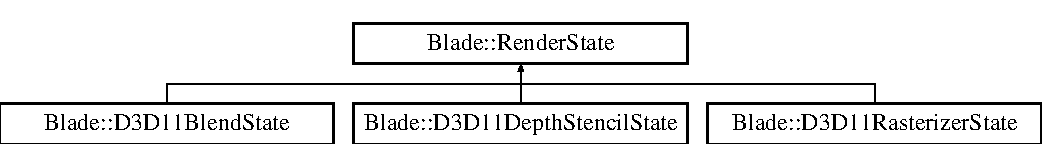
\includegraphics[height=1.904762cm]{class_blade_1_1_render_state}
\end{center}
\end{figure}
\subsection*{Public Member Functions}
\begin{DoxyCompactItemize}
\item 
\mbox{\Hypertarget{class_blade_1_1_render_state_abac049a80872a9fdaaa773e72c841a11}\label{class_blade_1_1_render_state_abac049a80872a9fdaaa773e72c841a11}} 
virtual void {\bfseries Set} () const noexcept=0
\end{DoxyCompactItemize}


The documentation for this class was generated from the following files\+:\begin{DoxyCompactItemize}
\item 
include/render\+\_\+state.\+h\item 
src/render\+\_\+state.\+cpp\end{DoxyCompactItemize}

\hypertarget{class_blade_1_1_render_state_manager}{}\section{Blade\+:\+:Render\+State\+Manager Class Reference}
\label{class_blade_1_1_render_state_manager}\index{Blade\+::\+Render\+State\+Manager@{Blade\+::\+Render\+State\+Manager}}
\subsection*{Public Member Functions}
\begin{DoxyCompactItemize}
\item 
\mbox{\Hypertarget{class_blade_1_1_render_state_manager_a0b26e9c469b8ec7289bb107effc95a8b}\label{class_blade_1_1_render_state_manager_a0b26e9c469b8ec7289bb107effc95a8b}} 
void {\bfseries Initialize} () noexcept
\item 
\mbox{\Hypertarget{class_blade_1_1_render_state_manager_a3d2ef6c7f65efe5dc738db1f66650f0f}\label{class_blade_1_1_render_state_manager_a3d2ef6c7f65efe5dc738db1f66650f0f}} 
void {\bfseries Set} (Render\+State\+Type render\+State) noexcept
\end{DoxyCompactItemize}


The documentation for this class was generated from the following files\+:\begin{DoxyCompactItemize}
\item 
include/render\+\_\+state\+\_\+manager.\+h\item 
src/render\+\_\+state\+\_\+manager.\+cpp\end{DoxyCompactItemize}

\hypertarget{class_blade_1_1_render_system}{}\section{Blade\+:\+:Render\+System Class Reference}
\label{class_blade_1_1_render_system}\index{Blade\+::\+Render\+System@{Blade\+::\+Render\+System}}


A \hyperlink{class_blade_1_1_system}{System} responsible for processing the Render\+Components by passing them through a specified pipeline.  




{\ttfamily \#include $<$render\+\_\+system.\+h$>$}

Inheritance diagram for Blade\+:\+:Render\+System\+:\begin{figure}[H]
\begin{center}
\leavevmode
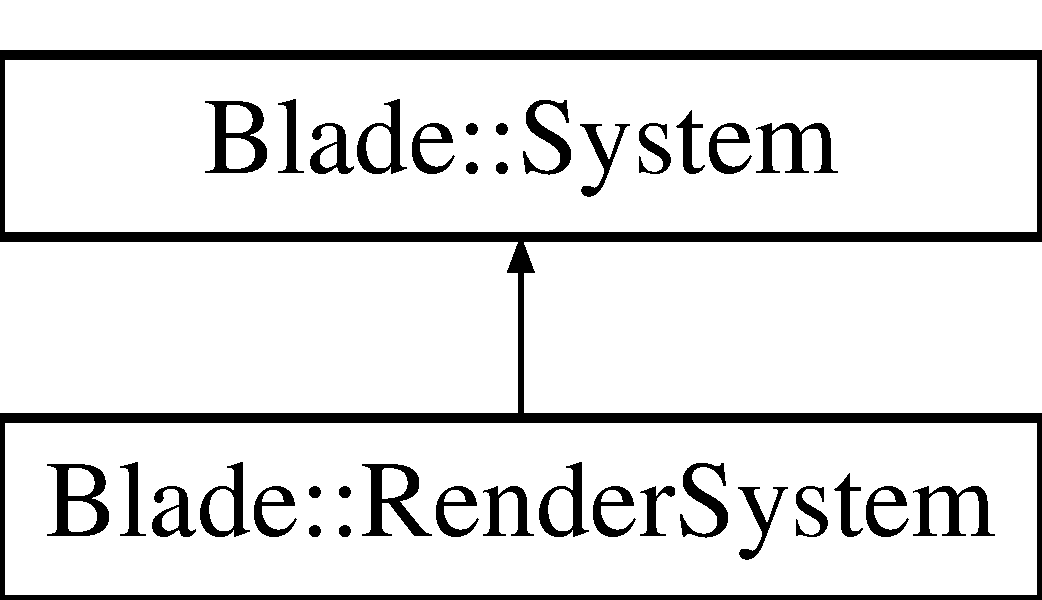
\includegraphics[height=2.000000cm]{class_blade_1_1_render_system}
\end{center}
\end{figure}
\subsection*{Public Member Functions}
\begin{DoxyCompactItemize}
\item 
\mbox{\Hypertarget{class_blade_1_1_render_system_a97b0fa28dab28db46175ceb47b229c13}\label{class_blade_1_1_render_system_a97b0fa28dab28db46175ceb47b229c13}} 
\hyperlink{class_blade_1_1_render_system_a97b0fa28dab28db46175ceb47b229c13}{$\sim$\+Render\+System} ()
\begin{DoxyCompactList}\small\item\em Destructor of the \hyperlink{class_blade_1_1_render_system}{Render\+System}. Deallocates the pipeline member. \end{DoxyCompactList}\item 
void \hyperlink{class_blade_1_1_render_system_a36ad263f137b6634542966dea0229047}{Register\+Component} (\hyperlink{class_blade_1_1_render_component}{Render\+Component} $\ast$render\+Component) noexcept
\begin{DoxyCompactList}\small\item\em Registeres a \hyperlink{class_blade_1_1_render_component}{Render\+Component} to the \hyperlink{class_blade_1_1_render_system}{Render\+System}. \end{DoxyCompactList}\item 
void \hyperlink{class_blade_1_1_render_system_afaaca8d329f9fa9903a28202959f8958}{Unregister\+Component} (int id) noexcept
\begin{DoxyCompactList}\small\item\em Unregisters a \hyperlink{class_blade_1_1_render_component}{Render\+Component} from the \hyperlink{class_blade_1_1_render_system}{Render\+System}. \end{DoxyCompactList}\item 
void \hyperlink{class_blade_1_1_render_system_a3d760ee1b6c5b4e6f9ec0892d948b91c}{Set\+Render\+Pass\+Pipeline} (Render\+Pass\+Pipeline $\ast$render\+Pass\+Pipeline) noexcept
\begin{DoxyCompactList}\small\item\em Sets the pipeline that the \hyperlink{class_blade_1_1_render_system}{Render\+System} will pass the Render\+Components through. \end{DoxyCompactList}\item 
\mbox{\Hypertarget{class_blade_1_1_render_system_a8f09fc8598972eacddd158fc14fc3cde}\label{class_blade_1_1_render_system_a8f09fc8598972eacddd158fc14fc3cde}} 
void \hyperlink{class_blade_1_1_render_system_a8f09fc8598972eacddd158fc14fc3cde}{Clear\+Render\+Pass\+Pipeline} () noexcept
\begin{DoxyCompactList}\small\item\em Removed the pipeline from the \hyperlink{class_blade_1_1_render_system}{Render\+System} if one is set. \end{DoxyCompactList}\item 
bool \hyperlink{class_blade_1_1_render_system_a476d3d55dcc9f65e8a88096aace6dcfc}{Initialize} () noexcept override
\begin{DoxyCompactList}\small\item\em Initializes the \hyperlink{class_blade_1_1_render_system}{Render\+System}. \end{DoxyCompactList}\item 
void \hyperlink{class_blade_1_1_render_system_a8edd0d0c9d5d54c395a03f98f6b16fb9}{Process} (float delta\+Time=.\+0f, long time=0) noexcept override
\begin{DoxyCompactList}\small\item\em Processes the Render\+Components by passing them through the Render\+Pass\+Pipeline. \end{DoxyCompactList}\item 
void \hyperlink{class_blade_1_1_render_system_a6bbc18b56812347c4960336f5d15effa}{Set\+Sorting} (bool sorting) noexcept
\begin{DoxyCompactList}\small\item\em Set the sorting flag. \end{DoxyCompactList}\end{DoxyCompactItemize}


\subsection{Detailed Description}
A \hyperlink{class_blade_1_1_system}{System} responsible for processing the Render\+Components by passing them through a specified pipeline. 

\subsection{Member Function Documentation}
\mbox{\Hypertarget{class_blade_1_1_render_system_a476d3d55dcc9f65e8a88096aace6dcfc}\label{class_blade_1_1_render_system_a476d3d55dcc9f65e8a88096aace6dcfc}} 
\index{Blade\+::\+Render\+System@{Blade\+::\+Render\+System}!Initialize@{Initialize}}
\index{Initialize@{Initialize}!Blade\+::\+Render\+System@{Blade\+::\+Render\+System}}
\subsubsection{\texorpdfstring{Initialize()}{Initialize()}}
{\footnotesize\ttfamily bool Blade\+::\+Render\+System\+::\+Initialize (\begin{DoxyParamCaption}{ }\end{DoxyParamCaption})\hspace{0.3cm}{\ttfamily [override]}, {\ttfamily [virtual]}, {\ttfamily [noexcept]}}



Initializes the \hyperlink{class_blade_1_1_render_system}{Render\+System}. 

\begin{DoxyReturn}{Returns}
T\+R\+UE if initialization is successfull, F\+A\+L\+SE otherwise. 
\end{DoxyReturn}


Implements \hyperlink{class_blade_1_1_system_a63fa00af40dc54d093300eff4785f26f}{Blade\+::\+System}.

\mbox{\Hypertarget{class_blade_1_1_render_system_a8edd0d0c9d5d54c395a03f98f6b16fb9}\label{class_blade_1_1_render_system_a8edd0d0c9d5d54c395a03f98f6b16fb9}} 
\index{Blade\+::\+Render\+System@{Blade\+::\+Render\+System}!Process@{Process}}
\index{Process@{Process}!Blade\+::\+Render\+System@{Blade\+::\+Render\+System}}
\subsubsection{\texorpdfstring{Process()}{Process()}}
{\footnotesize\ttfamily void Blade\+::\+Render\+System\+::\+Process (\begin{DoxyParamCaption}\item[{float}]{delta\+Time = {\ttfamily .0f},  }\item[{long}]{time = {\ttfamily 0} }\end{DoxyParamCaption})\hspace{0.3cm}{\ttfamily [override]}, {\ttfamily [virtual]}, {\ttfamily [noexcept]}}



Processes the Render\+Components by passing them through the Render\+Pass\+Pipeline. 


\begin{DoxyParams}{Parameters}
{\em delta\+Time} & The time elapsed from the previous frame of the application. \\
\hline
\end{DoxyParams}


Implements \hyperlink{class_blade_1_1_system_a80c186f5f9f8fa4fd317b861853fe6a8}{Blade\+::\+System}.

\mbox{\Hypertarget{class_blade_1_1_render_system_a36ad263f137b6634542966dea0229047}\label{class_blade_1_1_render_system_a36ad263f137b6634542966dea0229047}} 
\index{Blade\+::\+Render\+System@{Blade\+::\+Render\+System}!Register\+Component@{Register\+Component}}
\index{Register\+Component@{Register\+Component}!Blade\+::\+Render\+System@{Blade\+::\+Render\+System}}
\subsubsection{\texorpdfstring{Register\+Component()}{RegisterComponent()}}
{\footnotesize\ttfamily void Blade\+::\+Render\+System\+::\+Register\+Component (\begin{DoxyParamCaption}\item[{\hyperlink{class_blade_1_1_render_component}{Render\+Component} $\ast$}]{render\+Component }\end{DoxyParamCaption})\hspace{0.3cm}{\ttfamily [noexcept]}}



Registeres a \hyperlink{class_blade_1_1_render_component}{Render\+Component} to the \hyperlink{class_blade_1_1_render_system}{Render\+System}. 


\begin{DoxyParams}{Parameters}
{\em render\+Component} & The component to be registered to the Render\+Sytstem for processing. \\
\hline
\end{DoxyParams}
\mbox{\Hypertarget{class_blade_1_1_render_system_a3d760ee1b6c5b4e6f9ec0892d948b91c}\label{class_blade_1_1_render_system_a3d760ee1b6c5b4e6f9ec0892d948b91c}} 
\index{Blade\+::\+Render\+System@{Blade\+::\+Render\+System}!Set\+Render\+Pass\+Pipeline@{Set\+Render\+Pass\+Pipeline}}
\index{Set\+Render\+Pass\+Pipeline@{Set\+Render\+Pass\+Pipeline}!Blade\+::\+Render\+System@{Blade\+::\+Render\+System}}
\subsubsection{\texorpdfstring{Set\+Render\+Pass\+Pipeline()}{SetRenderPassPipeline()}}
{\footnotesize\ttfamily void Blade\+::\+Render\+System\+::\+Set\+Render\+Pass\+Pipeline (\begin{DoxyParamCaption}\item[{Render\+Pass\+Pipeline $\ast$}]{render\+Pass\+Pipeline }\end{DoxyParamCaption})\hspace{0.3cm}{\ttfamily [noexcept]}}



Sets the pipeline that the \hyperlink{class_blade_1_1_render_system}{Render\+System} will pass the Render\+Components through. 


\begin{DoxyParams}{Parameters}
{\em render\+Pass\+Pipeline} & The pipeline that processes the Render\+Components. \\
\hline
\end{DoxyParams}
\mbox{\Hypertarget{class_blade_1_1_render_system_a6bbc18b56812347c4960336f5d15effa}\label{class_blade_1_1_render_system_a6bbc18b56812347c4960336f5d15effa}} 
\index{Blade\+::\+Render\+System@{Blade\+::\+Render\+System}!Set\+Sorting@{Set\+Sorting}}
\index{Set\+Sorting@{Set\+Sorting}!Blade\+::\+Render\+System@{Blade\+::\+Render\+System}}
\subsubsection{\texorpdfstring{Set\+Sorting()}{SetSorting()}}
{\footnotesize\ttfamily void Blade\+::\+Render\+System\+::\+Set\+Sorting (\begin{DoxyParamCaption}\item[{bool}]{sorting }\end{DoxyParamCaption})\hspace{0.3cm}{\ttfamily [noexcept]}}



Set the sorting flag. 

If sorting is enable, the render components are sorted by alpha value. 
\begin{DoxyParams}{Parameters}
{\em sorting} & The sorting flag\+: T\+R\+UE enable sorting. \\
\hline
\end{DoxyParams}
\mbox{\Hypertarget{class_blade_1_1_render_system_afaaca8d329f9fa9903a28202959f8958}\label{class_blade_1_1_render_system_afaaca8d329f9fa9903a28202959f8958}} 
\index{Blade\+::\+Render\+System@{Blade\+::\+Render\+System}!Unregister\+Component@{Unregister\+Component}}
\index{Unregister\+Component@{Unregister\+Component}!Blade\+::\+Render\+System@{Blade\+::\+Render\+System}}
\subsubsection{\texorpdfstring{Unregister\+Component()}{UnregisterComponent()}}
{\footnotesize\ttfamily void Blade\+::\+Render\+System\+::\+Unregister\+Component (\begin{DoxyParamCaption}\item[{int}]{id }\end{DoxyParamCaption})\hspace{0.3cm}{\ttfamily [noexcept]}}



Unregisters a \hyperlink{class_blade_1_1_render_component}{Render\+Component} from the \hyperlink{class_blade_1_1_render_system}{Render\+System}. 


\begin{DoxyParams}{Parameters}
{\em id} & The unique id of the \hyperlink{class_blade_1_1_render_component}{Render\+Component} to be unregistered. \\
\hline
\end{DoxyParams}


The documentation for this class was generated from the following files\+:\begin{DoxyCompactItemize}
\item 
include/render\+\_\+system.\+h\item 
src/render\+\_\+system.\+cpp\end{DoxyCompactItemize}

\hypertarget{class_blade_1_1_render_target}{}\section{Blade\+:\+:Render\+Target Class Reference}
\label{class_blade_1_1_render_target}\index{Blade\+::\+Render\+Target@{Blade\+::\+Render\+Target}}
Inheritance diagram for Blade\+:\+:Render\+Target\+:\begin{figure}[H]
\begin{center}
\leavevmode
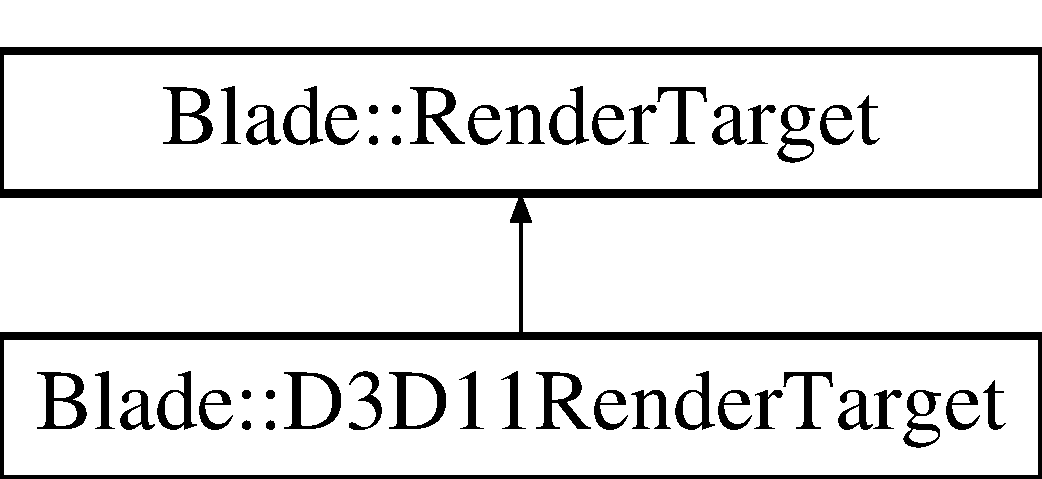
\includegraphics[height=2.000000cm]{class_blade_1_1_render_target}
\end{center}
\end{figure}
\subsection*{Public Member Functions}
\begin{DoxyCompactItemize}
\item 
\mbox{\Hypertarget{class_blade_1_1_render_target_acd9bdc4a28b22738e0963660f682bda7}\label{class_blade_1_1_render_target_acd9bdc4a28b22738e0963660f682bda7}} 
{\bfseries Render\+Target} (const Vec2i \&size)
\item 
\mbox{\Hypertarget{class_blade_1_1_render_target_a62aab69b1a6f7fce87ed6feeeef3ab46}\label{class_blade_1_1_render_target_a62aab69b1a6f7fce87ed6feeeef3ab46}} 
virtual bool {\bfseries Create} (const Vec2i \&size)=0
\item 
\mbox{\Hypertarget{class_blade_1_1_render_target_a32bdd25885d96b7c7621633190bbb545}\label{class_blade_1_1_render_target_a32bdd25885d96b7c7621633190bbb545}} 
virtual bool {\bfseries Bind} (Render\+Target\+Bind\+Type bind\+\_\+type) const =0
\item 
\mbox{\Hypertarget{class_blade_1_1_render_target_a51e464ab696fbf082b7b4d0281e46117}\label{class_blade_1_1_render_target_a51e464ab696fbf082b7b4d0281e46117}} 
virtual bool {\bfseries Unbind} () const =0
\item 
\mbox{\Hypertarget{class_blade_1_1_render_target_af11c64c3d361074ad8c879731b7cf3a8}\label{class_blade_1_1_render_target_af11c64c3d361074ad8c879731b7cf3a8}} 
void {\bfseries Set\+Size} (const Vec2i \&size) noexcept
\item 
\mbox{\Hypertarget{class_blade_1_1_render_target_aa041c7a923f9bba0f0d77ce349333792}\label{class_blade_1_1_render_target_aa041c7a923f9bba0f0d77ce349333792}} 
const Vec2i \& {\bfseries Get\+Size} () const noexcept
\end{DoxyCompactItemize}


The documentation for this class was generated from the following files\+:\begin{DoxyCompactItemize}
\item 
include/render\+\_\+target.\+h\item 
src/render\+\_\+target.\+cpp\end{DoxyCompactItemize}

\hypertarget{class_blade_1_1_resource}{}\section{Blade\+:\+:Resource Class Reference}
\label{class_blade_1_1_resource}\index{Blade\+::\+Resource@{Blade\+::\+Resource}}


\hyperlink{class_blade_1_1_resource}{Resource} class of the engine.  




{\ttfamily \#include $<$resource.\+h$>$}

Inheritance diagram for Blade\+:\+:Resource\+:\begin{figure}[H]
\begin{center}
\leavevmode
\includegraphics[height=1.548387cm]{class_blade_1_1_resource}
\end{center}
\end{figure}
\subsection*{Public Member Functions}
\begin{DoxyCompactItemize}
\item 
\mbox{\Hypertarget{class_blade_1_1_resource_aad67c68d5164726a1029c534fe7d003b}\label{class_blade_1_1_resource_aad67c68d5164726a1029c534fe7d003b}} 
{\bfseries Resource} (unsigned int id)
\item 
unsigned int \hyperlink{class_blade_1_1_resource_a2346c235601b0a703287bff9ad2c3432}{Get\+Id} () const noexcept
\begin{DoxyCompactList}\small\item\em Getter of the resource id. \end{DoxyCompactList}\item 
void \hyperlink{class_blade_1_1_resource_a76912ec0d2dfb35a5fffc7364b8a867d}{Set\+Id} (unsigned int id) noexcept
\begin{DoxyCompactList}\small\item\em Setter for the resource ID. \end{DoxyCompactList}\item 
virtual bool \hyperlink{class_blade_1_1_resource_ad89ab00a3b81df1338a8310ec92c5cff}{Load} (const std\+::wstring \&file\+\_\+name) noexcept=0
\begin{DoxyCompactList}\small\item\em Load a resource form a file. \end{DoxyCompactList}\end{DoxyCompactItemize}


\subsection{Detailed Description}
\hyperlink{class_blade_1_1_resource}{Resource} class of the engine. 

A resource is type agnostic. 

\subsection{Member Function Documentation}
\mbox{\Hypertarget{class_blade_1_1_resource_a2346c235601b0a703287bff9ad2c3432}\label{class_blade_1_1_resource_a2346c235601b0a703287bff9ad2c3432}} 
\index{Blade\+::\+Resource@{Blade\+::\+Resource}!Get\+Id@{Get\+Id}}
\index{Get\+Id@{Get\+Id}!Blade\+::\+Resource@{Blade\+::\+Resource}}
\subsubsection{\texorpdfstring{Get\+Id()}{GetId()}}
{\footnotesize\ttfamily unsigned int Blade\+::\+Resource\+::\+Get\+Id (\begin{DoxyParamCaption}{ }\end{DoxyParamCaption}) const\hspace{0.3cm}{\ttfamily [inline]}, {\ttfamily [noexcept]}}



Getter of the resource id. 

\begin{DoxyReturn}{Returns}
\hyperlink{class_blade_1_1_resource}{Resource} ID 
\end{DoxyReturn}
\mbox{\Hypertarget{class_blade_1_1_resource_ad89ab00a3b81df1338a8310ec92c5cff}\label{class_blade_1_1_resource_ad89ab00a3b81df1338a8310ec92c5cff}} 
\index{Blade\+::\+Resource@{Blade\+::\+Resource}!Load@{Load}}
\index{Load@{Load}!Blade\+::\+Resource@{Blade\+::\+Resource}}
\subsubsection{\texorpdfstring{Load()}{Load()}}
{\footnotesize\ttfamily virtual bool Blade\+::\+Resource\+::\+Load (\begin{DoxyParamCaption}\item[{const std\+::wstring \&}]{file\+\_\+name }\end{DoxyParamCaption})\hspace{0.3cm}{\ttfamily [pure virtual]}, {\ttfamily [noexcept]}}



Load a resource form a file. 


\begin{DoxyParams}{Parameters}
{\em file\+\_\+name} & The path of the file where the resource is stored. \\
\hline
\end{DoxyParams}
\begin{DoxyReturn}{Returns}
T\+R\+UE if the loading has been successful, false otherwise. 
\end{DoxyReturn}


Implemented in \hyperlink{class_blade_1_1_entity_a1e23e9402a5c5a1d266c208c7637c539}{Blade\+::\+Entity}, \hyperlink{class_blade_1_1_mesh_a999b87101e849d8a6618d95c69387ec1}{Blade\+::\+Mesh}, \hyperlink{struct_blade_1_1_emitter_descriptor_ac3bf4ccedee573630235f498a0c47822}{Blade\+::\+Emitter\+Descriptor}, \hyperlink{class_blade_1_1_d3_d11_shader_a713231594415a37d484f115478acf084}{Blade\+::\+D3\+D11\+Shader}, \hyperlink{class_blade_1_1_d3_d11_texture_ae9f6d01709ba9db4085cf6b3d90b3ac7}{Blade\+::\+D3\+D11\+Texture}, and \hyperlink{class_blade_1_1_audio_sample_a27bc4a11067251a2c820f1e3096bb812}{Blade\+::\+Audio\+Sample}.

\mbox{\Hypertarget{class_blade_1_1_resource_a76912ec0d2dfb35a5fffc7364b8a867d}\label{class_blade_1_1_resource_a76912ec0d2dfb35a5fffc7364b8a867d}} 
\index{Blade\+::\+Resource@{Blade\+::\+Resource}!Set\+Id@{Set\+Id}}
\index{Set\+Id@{Set\+Id}!Blade\+::\+Resource@{Blade\+::\+Resource}}
\subsubsection{\texorpdfstring{Set\+Id()}{SetId()}}
{\footnotesize\ttfamily void Blade\+::\+Resource\+::\+Set\+Id (\begin{DoxyParamCaption}\item[{unsigned int}]{id }\end{DoxyParamCaption})\hspace{0.3cm}{\ttfamily [inline]}, {\ttfamily [noexcept]}}



Setter for the resource ID. 


\begin{DoxyParams}{Parameters}
{\em id} & the resource ID \\
\hline
\end{DoxyParams}


The documentation for this class was generated from the following files\+:\begin{DoxyCompactItemize}
\item 
include/resource.\+h\item 
src/resource.\+cpp\end{DoxyCompactItemize}

\hypertarget{class_blade_1_1_resource_manager}{}\section{Blade\+:\+:Resource\+Manager Class Reference}
\label{class_blade_1_1_resource_manager}\index{Blade\+::\+Resource\+Manager@{Blade\+::\+Resource\+Manager}}
\subsection*{Public Member Functions}
\begin{DoxyCompactItemize}
\item 
\mbox{\Hypertarget{class_blade_1_1_resource_manager_ad99695e0e3d6cf66e3645b61dcede9b8}\label{class_blade_1_1_resource_manager_ad99695e0e3d6cf66e3645b61dcede9b8}} 
{\footnotesize template$<$typename T $>$ }\\bool {\bfseries Load} (const std\+::wstring \&file\+Name)
\item 
\mbox{\Hypertarget{class_blade_1_1_resource_manager_a84e678264f844a6b4bca8d46ee16336b}\label{class_blade_1_1_resource_manager_a84e678264f844a6b4bca8d46ee16336b}} 
{\footnotesize template$<$typename T $>$ }\\T $\ast$ {\bfseries Get} (const std\+::wstring \&file\+Name)
\item 
\mbox{\Hypertarget{class_blade_1_1_resource_manager_aa406f90716a7758669b424a290549256}\label{class_blade_1_1_resource_manager_aa406f90716a7758669b424a290549256}} 
void {\bfseries Register\+Resource} (\hyperlink{class_blade_1_1_resource}{Resource} $\ast$resource, const std\+::wstring \&name)
\end{DoxyCompactItemize}


The documentation for this class was generated from the following file\+:\begin{DoxyCompactItemize}
\item 
include/resource\+\_\+manager.\+h\end{DoxyCompactItemize}

\hypertarget{class_blade_1_1_math_utils_1_1_runge_kutta4_integrator}{}\section{Blade\+:\+:Math\+Utils\+:\+:Runge\+Kutta4\+Integrator Class Reference}
\label{class_blade_1_1_math_utils_1_1_runge_kutta4_integrator}\index{Blade\+::\+Math\+Utils\+::\+Runge\+Kutta4\+Integrator@{Blade\+::\+Math\+Utils\+::\+Runge\+Kutta4\+Integrator}}
\subsection*{Static Public Member Functions}
\begin{DoxyCompactItemize}
\item 
\mbox{\Hypertarget{class_blade_1_1_math_utils_1_1_runge_kutta4_integrator_ac3f3e8e7203695a4511b1935837d49f3}\label{class_blade_1_1_math_utils_1_1_runge_kutta4_integrator_ac3f3e8e7203695a4511b1935837d49f3}} 
static void {\bfseries Integrate} (Vec3f \&position, Vec3f \&velocity, const Vec3f \&force, float mass, float time\+Sec, float delta\+Time) noexcept
\end{DoxyCompactItemize}


The documentation for this class was generated from the following files\+:\begin{DoxyCompactItemize}
\item 
include/math\+\_\+utils.\+h\item 
src/math\+\_\+utils.\+cpp\end{DoxyCompactItemize}

\hypertarget{struct_blade_1_1_sample_playlist}{}\section{Blade\+:\+:Sample\+Playlist Struct Reference}
\label{struct_blade_1_1_sample_playlist}\index{Blade\+::\+Sample\+Playlist@{Blade\+::\+Sample\+Playlist}}
\subsection*{Public Attributes}
\begin{DoxyCompactItemize}
\item 
\mbox{\Hypertarget{struct_blade_1_1_sample_playlist_ad67c205beb8523f9019eb9777536f3bb}\label{struct_blade_1_1_sample_playlist_ad67c205beb8523f9019eb9777536f3bb}} 
std\+::list$<$ \hyperlink{class_blade_1_1_audio_sample}{Audio\+Sample} $\ast$ $>$ {\bfseries samples}
\item 
\mbox{\Hypertarget{struct_blade_1_1_sample_playlist_a75e205b1ccd51e8840728b68a5dbc85e}\label{struct_blade_1_1_sample_playlist_a75e205b1ccd51e8840728b68a5dbc85e}} 
std\+::list$<$ \hyperlink{class_blade_1_1_audio_sample}{Audio\+Sample} $\ast$ $>$\+::iterator {\bfseries it}
\item 
\mbox{\Hypertarget{struct_blade_1_1_sample_playlist_acb96f5c75868058ceac436b1033c7d00}\label{struct_blade_1_1_sample_playlist_acb96f5c75868058ceac436b1033c7d00}} 
bool {\bfseries loop}
\item 
\mbox{\Hypertarget{struct_blade_1_1_sample_playlist_a7b32dc1e9b8095aba5cfd5453a353853}\label{struct_blade_1_1_sample_playlist_a7b32dc1e9b8095aba5cfd5453a353853}} 
bool {\bfseries started} \{ false \}
\item 
\mbox{\Hypertarget{struct_blade_1_1_sample_playlist_a8253ce5a7fb4637abc1998e7575b16b2}\label{struct_blade_1_1_sample_playlist_a8253ce5a7fb4637abc1998e7575b16b2}} 
int {\bfseries source\+\_\+idx} \{ -\/1 \}
\end{DoxyCompactItemize}


The documentation for this struct was generated from the following files\+:\begin{DoxyCompactItemize}
\item 
include/audio\+\_\+manager.\+h\item 
src/audio\+\_\+manager.\+cpp\end{DoxyCompactItemize}

\hypertarget{class_blade_1_1_scene}{}\section{Blade\+:\+:Scene Class Reference}
\label{class_blade_1_1_scene}\index{Blade\+::\+Scene@{Blade\+::\+Scene}}
\subsection*{Public Member Functions}
\begin{DoxyCompactItemize}
\item 
\mbox{\Hypertarget{class_blade_1_1_scene_a80a9bba828a6faf60ca9a91301e6e707}\label{class_blade_1_1_scene_a80a9bba828a6faf60ca9a91301e6e707}} 
{\bfseries Scene} (const \hyperlink{class_blade_1_1_scene}{Scene} \&other)=delete
\item 
\mbox{\Hypertarget{class_blade_1_1_scene_ae2d9a202f00b35daf25d8bb7acbb8b16}\label{class_blade_1_1_scene_ae2d9a202f00b35daf25d8bb7acbb8b16}} 
\hyperlink{class_blade_1_1_scene}{Scene} \& {\bfseries operator=} (const \hyperlink{class_blade_1_1_scene}{Scene} \&other)=delete
\item 
\mbox{\Hypertarget{class_blade_1_1_scene_a0bd508e8d4ab8db0b91eb8959056bb93}\label{class_blade_1_1_scene_a0bd508e8d4ab8db0b91eb8959056bb93}} 
virtual bool {\bfseries Initialize} ()=0
\item 
\mbox{\Hypertarget{class_blade_1_1_scene_a0f17cd32cb502502fd5a3a39c72b4856}\label{class_blade_1_1_scene_a0f17cd32cb502502fd5a3a39c72b4856}} 
void {\bfseries Add\+Entity} (\hyperlink{class_blade_1_1_entity}{Entity} $\ast$object) noexcept
\item 
\mbox{\Hypertarget{class_blade_1_1_scene_ae04a504f28ab2c80099863d067cb6914}\label{class_blade_1_1_scene_ae04a504f28ab2c80099863d067cb6914}} 
void {\bfseries Remove\+Entity} (const std\+::string \&name) noexcept
\item 
\mbox{\Hypertarget{class_blade_1_1_scene_a41c8f3a8a59307c42a17163614ba8dd8}\label{class_blade_1_1_scene_a41c8f3a8a59307c42a17163614ba8dd8}} 
void {\bfseries Remove\+Entities} () noexcept
\item 
\mbox{\Hypertarget{class_blade_1_1_scene_abd8993ff5deae13c05bfcdffbe9af6ff}\label{class_blade_1_1_scene_abd8993ff5deae13c05bfcdffbe9af6ff}} 
const std\+::vector$<$ \hyperlink{class_blade_1_1_entity}{Entity} $\ast$ $>$ \& {\bfseries Get\+Entities} () const noexcept
\item 
\mbox{\Hypertarget{class_blade_1_1_scene_a4aa00824c68cf68734f85ac465796385}\label{class_blade_1_1_scene_a4aa00824c68cf68734f85ac465796385}} 
\hyperlink{class_blade_1_1_entity}{Entity} $\ast$ {\bfseries Get\+Entity\+By\+Name} (const std\+::string \&name) noexcept
\item 
\mbox{\Hypertarget{class_blade_1_1_scene_abb80a0590b4d723b5f13ec8c488e513a}\label{class_blade_1_1_scene_abb80a0590b4d723b5f13ec8c488e513a}} 
virtual void {\bfseries On\+Key\+Down} (unsigned char key, int x, int y) noexcept=0
\item 
\mbox{\Hypertarget{class_blade_1_1_scene_abe25ad91527c82b56409be7097afbf49}\label{class_blade_1_1_scene_abe25ad91527c82b56409be7097afbf49}} 
virtual void {\bfseries On\+Key\+Up} (unsigned char key, int x, int y) noexcept=0
\item 
\mbox{\Hypertarget{class_blade_1_1_scene_aa0296f990fc1cacbfc97f657d6cb958f}\label{class_blade_1_1_scene_aa0296f990fc1cacbfc97f657d6cb958f}} 
virtual void {\bfseries On\+Mouse\+Motion} (int x, int y) noexcept=0
\item 
\mbox{\Hypertarget{class_blade_1_1_scene_ab54558db189ce57505ede242ffc303d2}\label{class_blade_1_1_scene_ab54558db189ce57505ede242ffc303d2}} 
virtual void {\bfseries On\+Mouse\+Click} (int button, bool state, int x, int y) noexcept=0
\item 
\mbox{\Hypertarget{class_blade_1_1_scene_a657797f1b08ac81bea28a2f9ed0e9c6f}\label{class_blade_1_1_scene_a657797f1b08ac81bea28a2f9ed0e9c6f}} 
virtual void {\bfseries Update} (float delta\+Time, long time=0) noexcept
\item 
\mbox{\Hypertarget{class_blade_1_1_scene_ad1e610e1b5ea1cc4c6eaeac74e1c365b}\label{class_blade_1_1_scene_ad1e610e1b5ea1cc4c6eaeac74e1c365b}} 
virtual void {\bfseries Draw} () const noexcept=0
\item 
\mbox{\Hypertarget{class_blade_1_1_scene_ac49cdbb30d13096320971ef9389d0a54}\label{class_blade_1_1_scene_ac49cdbb30d13096320971ef9389d0a54}} 
virtual void {\bfseries On\+Message} (const \hyperlink{class_blade_1_1_ref_counted_container}{Message\+Container}$<$ std\+::string $>$ \&msg) const noexcept
\end{DoxyCompactItemize}


The documentation for this class was generated from the following files\+:\begin{DoxyCompactItemize}
\item 
include/scene.\+h\item 
src/scene.\+cpp\end{DoxyCompactItemize}

\hypertarget{class_blade_1_1_scene_manager}{}\section{Blade\+:\+:Scene\+Manager Class Reference}
\label{class_blade_1_1_scene_manager}\index{Blade\+::\+Scene\+Manager@{Blade\+::\+Scene\+Manager}}


\hyperlink{class_blade_1_1_scene}{Scene} manager of the engine.  




{\ttfamily \#include $<$scene\+\_\+manager.\+h$>$}

\subsection*{Public Member Functions}
\begin{DoxyCompactItemize}
\item 
bool \hyperlink{class_blade_1_1_scene_manager_a3bdd62a565c3b39bb0ae0399f16b36d5}{Push\+Scene} (std\+::unique\+\_\+ptr$<$ \hyperlink{class_blade_1_1_scene}{Scene} $>$ scene) noexcept
\begin{DoxyCompactList}\small\item\em Push a new scene in the manager. \end{DoxyCompactList}\item 
\mbox{\Hypertarget{class_blade_1_1_scene_manager_af71cf80bd23a9b708abccd58c110c183}\label{class_blade_1_1_scene_manager_af71cf80bd23a9b708abccd58c110c183}} 
void \hyperlink{class_blade_1_1_scene_manager_af71cf80bd23a9b708abccd58c110c183}{Pop\+Scene} () noexcept
\begin{DoxyCompactList}\small\item\em Pop a scene to the manager. \end{DoxyCompactList}\item 
void \hyperlink{class_blade_1_1_scene_manager_a58a554c9fbce22aa0e09b51d4811f9fe}{On\+Key\+Down} (unsigned char key, int x, int y) noexcept
\begin{DoxyCompactList}\small\item\em Propagate Key\+Down information to the active scene. \end{DoxyCompactList}\item 
void \hyperlink{class_blade_1_1_scene_manager_ad2841ecb96bdfc11134e365ae2f8eb51}{On\+Key\+Up} (unsigned char key, int x, int y) noexcept
\begin{DoxyCompactList}\small\item\em Propagate Key\+Up information to the active scene. \end{DoxyCompactList}\item 
void \hyperlink{class_blade_1_1_scene_manager_a38dfdd6584e00fbf5b5181cc772b8050}{On\+Mouse\+Motion} (int x, int y) noexcept
\begin{DoxyCompactList}\small\item\em Propagate the mouse position to the active scene. \end{DoxyCompactList}\item 
void \hyperlink{class_blade_1_1_scene_manager_a2dc0c80a65f765e2ef4ac4ca69b9231e}{On\+Mouse\+Click} (int button, bool state, int x, int y) noexcept
\begin{DoxyCompactList}\small\item\em Propagate mouse click to the active scene. \end{DoxyCompactList}\item 
void \hyperlink{class_blade_1_1_scene_manager_ae0bc94af4c9686236c90d2a9a6529062}{On\+Message} (const \hyperlink{class_blade_1_1_ref_counted_container}{Message\+Container}$<$ std\+::string $>$ \&msg) noexcept
\begin{DoxyCompactList}\small\item\em Propagate the message from the application to the scene. \end{DoxyCompactList}\item 
void \hyperlink{class_blade_1_1_scene_manager_a68f1c083b875be3634870758ee697792}{Update} (float delta\+\_\+time, long time) noexcept
\begin{DoxyCompactList}\small\item\em Calls update on the current scene. \end{DoxyCompactList}\item 
\mbox{\Hypertarget{class_blade_1_1_scene_manager_a6e393993821909643377f638766a3cf9}\label{class_blade_1_1_scene_manager_a6e393993821909643377f638766a3cf9}} 
void \hyperlink{class_blade_1_1_scene_manager_a6e393993821909643377f638766a3cf9}{Draw} () noexcept
\begin{DoxyCompactList}\small\item\em Draw the current scene. \end{DoxyCompactList}\item 
\mbox{\Hypertarget{class_blade_1_1_scene_manager_a52232b73f5749916a22b6cf01707140e}\label{class_blade_1_1_scene_manager_a52232b73f5749916a22b6cf01707140e}} 
\hyperlink{class_blade_1_1_scene}{Scene} $\ast$ \hyperlink{class_blade_1_1_scene_manager_a52232b73f5749916a22b6cf01707140e}{Get\+Current\+Scene} () const noexcept
\begin{DoxyCompactList}\small\item\em Returns the current scene. \end{DoxyCompactList}\end{DoxyCompactItemize}


\subsection{Detailed Description}
\hyperlink{class_blade_1_1_scene}{Scene} manager of the engine. 

Stores the collection of scenes and implement a F\+SM paradigm. 

\subsection{Member Function Documentation}
\mbox{\Hypertarget{class_blade_1_1_scene_manager_a58a554c9fbce22aa0e09b51d4811f9fe}\label{class_blade_1_1_scene_manager_a58a554c9fbce22aa0e09b51d4811f9fe}} 
\index{Blade\+::\+Scene\+Manager@{Blade\+::\+Scene\+Manager}!On\+Key\+Down@{On\+Key\+Down}}
\index{On\+Key\+Down@{On\+Key\+Down}!Blade\+::\+Scene\+Manager@{Blade\+::\+Scene\+Manager}}
\subsubsection{\texorpdfstring{On\+Key\+Down()}{OnKeyDown()}}
{\footnotesize\ttfamily void Blade\+::\+Scene\+Manager\+::\+On\+Key\+Down (\begin{DoxyParamCaption}\item[{unsigned char}]{key,  }\item[{int}]{x,  }\item[{int}]{y }\end{DoxyParamCaption})\hspace{0.3cm}{\ttfamily [noexcept]}}



Propagate Key\+Down information to the active scene. 


\begin{DoxyParams}{Parameters}
{\em key} & the pressed \\
\hline
{\em x} & The x value \\
\hline
{\em y} & The y value \\
\hline
\end{DoxyParams}
\mbox{\Hypertarget{class_blade_1_1_scene_manager_ad2841ecb96bdfc11134e365ae2f8eb51}\label{class_blade_1_1_scene_manager_ad2841ecb96bdfc11134e365ae2f8eb51}} 
\index{Blade\+::\+Scene\+Manager@{Blade\+::\+Scene\+Manager}!On\+Key\+Up@{On\+Key\+Up}}
\index{On\+Key\+Up@{On\+Key\+Up}!Blade\+::\+Scene\+Manager@{Blade\+::\+Scene\+Manager}}
\subsubsection{\texorpdfstring{On\+Key\+Up()}{OnKeyUp()}}
{\footnotesize\ttfamily void Blade\+::\+Scene\+Manager\+::\+On\+Key\+Up (\begin{DoxyParamCaption}\item[{unsigned char}]{key,  }\item[{int}]{x,  }\item[{int}]{y }\end{DoxyParamCaption})\hspace{0.3cm}{\ttfamily [noexcept]}}



Propagate Key\+Up information to the active scene. 


\begin{DoxyParams}{Parameters}
{\em key} & the pressed \\
\hline
{\em x} & The x value \\
\hline
{\em y} & The y value \\
\hline
\end{DoxyParams}
\mbox{\Hypertarget{class_blade_1_1_scene_manager_ae0bc94af4c9686236c90d2a9a6529062}\label{class_blade_1_1_scene_manager_ae0bc94af4c9686236c90d2a9a6529062}} 
\index{Blade\+::\+Scene\+Manager@{Blade\+::\+Scene\+Manager}!On\+Message@{On\+Message}}
\index{On\+Message@{On\+Message}!Blade\+::\+Scene\+Manager@{Blade\+::\+Scene\+Manager}}
\subsubsection{\texorpdfstring{On\+Message()}{OnMessage()}}
{\footnotesize\ttfamily void Blade\+::\+Scene\+Manager\+::\+On\+Message (\begin{DoxyParamCaption}\item[{const \hyperlink{class_blade_1_1_ref_counted_container}{Message\+Container}$<$ std\+::string $>$ \&}]{msg }\end{DoxyParamCaption})\hspace{0.3cm}{\ttfamily [noexcept]}}



Propagate the message from the application to the scene. 


\begin{DoxyParams}{Parameters}
{\em msg} & The message. \\
\hline
\end{DoxyParams}
\mbox{\Hypertarget{class_blade_1_1_scene_manager_a2dc0c80a65f765e2ef4ac4ca69b9231e}\label{class_blade_1_1_scene_manager_a2dc0c80a65f765e2ef4ac4ca69b9231e}} 
\index{Blade\+::\+Scene\+Manager@{Blade\+::\+Scene\+Manager}!On\+Mouse\+Click@{On\+Mouse\+Click}}
\index{On\+Mouse\+Click@{On\+Mouse\+Click}!Blade\+::\+Scene\+Manager@{Blade\+::\+Scene\+Manager}}
\subsubsection{\texorpdfstring{On\+Mouse\+Click()}{OnMouseClick()}}
{\footnotesize\ttfamily void Blade\+::\+Scene\+Manager\+::\+On\+Mouse\+Click (\begin{DoxyParamCaption}\item[{int}]{button,  }\item[{bool}]{state,  }\item[{int}]{x,  }\item[{int}]{y }\end{DoxyParamCaption})\hspace{0.3cm}{\ttfamily [noexcept]}}



Propagate mouse click to the active scene. 


\begin{DoxyParams}{Parameters}
{\em button} & The button clicked \\
\hline
{\em state} & The state of the button\+: true = clicked \\
\hline
{\em x} & The x value of the mouse position relative to the window. \\
\hline
{\em y} & The y value of the mouse position relative to the window. \\
\hline
\end{DoxyParams}
\mbox{\Hypertarget{class_blade_1_1_scene_manager_a38dfdd6584e00fbf5b5181cc772b8050}\label{class_blade_1_1_scene_manager_a38dfdd6584e00fbf5b5181cc772b8050}} 
\index{Blade\+::\+Scene\+Manager@{Blade\+::\+Scene\+Manager}!On\+Mouse\+Motion@{On\+Mouse\+Motion}}
\index{On\+Mouse\+Motion@{On\+Mouse\+Motion}!Blade\+::\+Scene\+Manager@{Blade\+::\+Scene\+Manager}}
\subsubsection{\texorpdfstring{On\+Mouse\+Motion()}{OnMouseMotion()}}
{\footnotesize\ttfamily void Blade\+::\+Scene\+Manager\+::\+On\+Mouse\+Motion (\begin{DoxyParamCaption}\item[{int}]{x,  }\item[{int}]{y }\end{DoxyParamCaption})\hspace{0.3cm}{\ttfamily [noexcept]}}



Propagate the mouse position to the active scene. 


\begin{DoxyParams}{Parameters}
{\em x} & The x value of the mouse position relative to the window. \\
\hline
{\em y} & The y value of the mouse position relative to the window. \\
\hline
\end{DoxyParams}
\mbox{\Hypertarget{class_blade_1_1_scene_manager_a3bdd62a565c3b39bb0ae0399f16b36d5}\label{class_blade_1_1_scene_manager_a3bdd62a565c3b39bb0ae0399f16b36d5}} 
\index{Blade\+::\+Scene\+Manager@{Blade\+::\+Scene\+Manager}!Push\+Scene@{Push\+Scene}}
\index{Push\+Scene@{Push\+Scene}!Blade\+::\+Scene\+Manager@{Blade\+::\+Scene\+Manager}}
\subsubsection{\texorpdfstring{Push\+Scene()}{PushScene()}}
{\footnotesize\ttfamily bool Blade\+::\+Scene\+Manager\+::\+Push\+Scene (\begin{DoxyParamCaption}\item[{std\+::unique\+\_\+ptr$<$ \hyperlink{class_blade_1_1_scene}{Scene} $>$}]{scene }\end{DoxyParamCaption})\hspace{0.3cm}{\ttfamily [noexcept]}}



Push a new scene in the manager. 


\begin{DoxyParams}{Parameters}
{\em scene} & The new scene to push.\\
\hline
\end{DoxyParams}
The scene in the back is the active one. \mbox{\Hypertarget{class_blade_1_1_scene_manager_a68f1c083b875be3634870758ee697792}\label{class_blade_1_1_scene_manager_a68f1c083b875be3634870758ee697792}} 
\index{Blade\+::\+Scene\+Manager@{Blade\+::\+Scene\+Manager}!Update@{Update}}
\index{Update@{Update}!Blade\+::\+Scene\+Manager@{Blade\+::\+Scene\+Manager}}
\subsubsection{\texorpdfstring{Update()}{Update()}}
{\footnotesize\ttfamily void Blade\+::\+Scene\+Manager\+::\+Update (\begin{DoxyParamCaption}\item[{float}]{delta\+\_\+time,  }\item[{long}]{time }\end{DoxyParamCaption})\hspace{0.3cm}{\ttfamily [noexcept]}}



Calls update on the current scene. 


\begin{DoxyParams}{Parameters}
{\em delta\+\_\+time} & The delta time \\
\hline
{\em time} & The seconds since the application startup \\
\hline
\end{DoxyParams}


The documentation for this class was generated from the following files\+:\begin{DoxyCompactItemize}
\item 
include/scene\+\_\+manager.\+h\item 
src/scene\+\_\+manager.\+cpp\end{DoxyCompactItemize}

\hypertarget{class_blade_1_1_serializable}{}\section{Blade\+:\+:Serializable Class Reference}
\label{class_blade_1_1_serializable}\index{Blade\+::\+Serializable@{Blade\+::\+Serializable}}
Inheritance diagram for Blade\+:\+:Serializable\+:\begin{figure}[H]
\begin{center}
\leavevmode
\includegraphics[height=2.000000cm]{class_blade_1_1_serializable}
\end{center}
\end{figure}
\subsection*{Public Member Functions}
\begin{DoxyCompactItemize}
\item 
\mbox{\Hypertarget{class_blade_1_1_serializable_a0ae79c24827f91f620f9c267f17f1088}\label{class_blade_1_1_serializable_a0ae79c24827f91f620f9c267f17f1088}} 
virtual std\+::vector$<$ Byte $>$ {\bfseries Serialize} () noexcept=0
\end{DoxyCompactItemize}


The documentation for this class was generated from the following file\+:\begin{DoxyCompactItemize}
\item 
include/serializable.\+h\end{DoxyCompactItemize}

\hypertarget{class_blade_1_1_shader}{}\section{Blade\+:\+:Shader Class Reference}
\label{class_blade_1_1_shader}\index{Blade\+::\+Shader@{Blade\+::\+Shader}}
Inheritance diagram for Blade\+:\+:Shader\+:\begin{figure}[H]
\begin{center}
\leavevmode
\includegraphics[height=3.000000cm]{class_blade_1_1_shader}
\end{center}
\end{figure}
\subsection*{Additional Inherited Members}


The documentation for this class was generated from the following file\+:\begin{DoxyCompactItemize}
\item 
include/shader.\+h\end{DoxyCompactItemize}

\hypertarget{class_blade_1_1_shader_program}{}\section{Blade\+:\+:Shader\+Program Class Reference}
\label{class_blade_1_1_shader_program}\index{Blade\+::\+Shader\+Program@{Blade\+::\+Shader\+Program}}
Inheritance diagram for Blade\+:\+:Shader\+Program\+:\begin{figure}[H]
\begin{center}
\leavevmode
\includegraphics[height=2.000000cm]{class_blade_1_1_shader_program}
\end{center}
\end{figure}
\subsection*{Public Member Functions}
\begin{DoxyCompactItemize}
\item 
\mbox{\Hypertarget{class_blade_1_1_shader_program_a8d7453ddbb33f55af0bdc8deeb822560}\label{class_blade_1_1_shader_program_a8d7453ddbb33f55af0bdc8deeb822560}} 
{\bfseries Shader\+Program} (const \hyperlink{class_blade_1_1_shader_program}{Shader\+Program} \&)=default
\item 
\mbox{\Hypertarget{class_blade_1_1_shader_program_a4523ce6c51b414a9a5648eed51b3975c}\label{class_blade_1_1_shader_program_a4523ce6c51b414a9a5648eed51b3975c}} 
\hyperlink{class_blade_1_1_shader_program}{Shader\+Program} \& {\bfseries operator=} (const \hyperlink{class_blade_1_1_shader_program}{Shader\+Program} \&)=default
\item 
\mbox{\Hypertarget{class_blade_1_1_shader_program_af0a3a04d13e11d7ace44076c6346703e}\label{class_blade_1_1_shader_program_af0a3a04d13e11d7ace44076c6346703e}} 
virtual bool {\bfseries Create} (const \hyperlink{struct_blade_1_1_shader_program_desc}{Shader\+Program\+Desc} \&shader\+Program\+Desc) noexcept=0
\item 
\mbox{\Hypertarget{class_blade_1_1_shader_program_a826f4a4372ee7ba04d22e4bc4ee76d98}\label{class_blade_1_1_shader_program_a826f4a4372ee7ba04d22e4bc4ee76d98}} 
virtual void {\bfseries Bind} () const noexcept=0
\end{DoxyCompactItemize}


The documentation for this class was generated from the following files\+:\begin{DoxyCompactItemize}
\item 
include/shader\+\_\+program.\+h\item 
src/shader\+\_\+program.\+cpp\end{DoxyCompactItemize}

\hypertarget{struct_blade_1_1_shader_program_desc}{}\section{Blade\+:\+:Shader\+Program\+Desc Struct Reference}
\label{struct_blade_1_1_shader_program_desc}\index{Blade\+::\+Shader\+Program\+Desc@{Blade\+::\+Shader\+Program\+Desc}}
\subsection*{Public Attributes}
\begin{DoxyCompactItemize}
\item 
\mbox{\Hypertarget{struct_blade_1_1_shader_program_desc_a45ca89cb30d1fa353fd31da28239ec9b}\label{struct_blade_1_1_shader_program_desc_a45ca89cb30d1fa353fd31da28239ec9b}} 
std\+::string {\bfseries name}
\item 
\mbox{\Hypertarget{struct_blade_1_1_shader_program_desc_adab308bc4740327603d25d5e37e8b9fc}\label{struct_blade_1_1_shader_program_desc_adab308bc4740327603d25d5e37e8b9fc}} 
unsigned int {\bfseries input\+Layout\+Mask}
\item 
\mbox{\Hypertarget{struct_blade_1_1_shader_program_desc_aeb9a39fcdf32e7d6fc5a4d4ad8b78cab}\label{struct_blade_1_1_shader_program_desc_aeb9a39fcdf32e7d6fc5a4d4ad8b78cab}} 
std\+::wstring {\bfseries vertex\+Shader}
\item 
\mbox{\Hypertarget{struct_blade_1_1_shader_program_desc_a80ec11b4720427f20c426bd4c9c6d0b0}\label{struct_blade_1_1_shader_program_desc_a80ec11b4720427f20c426bd4c9c6d0b0}} 
std\+::wstring {\bfseries fragment\+Shader}
\item 
\mbox{\Hypertarget{struct_blade_1_1_shader_program_desc_a05b02c94d7d67dd35b889f6deb7a2d48}\label{struct_blade_1_1_shader_program_desc_a05b02c94d7d67dd35b889f6deb7a2d48}} 
std\+::wstring {\bfseries hull\+Shader}
\item 
\mbox{\Hypertarget{struct_blade_1_1_shader_program_desc_a60c1aff8d3a268bd11f747949e0d1442}\label{struct_blade_1_1_shader_program_desc_a60c1aff8d3a268bd11f747949e0d1442}} 
std\+::wstring {\bfseries domain\+Shader}
\item 
\mbox{\Hypertarget{struct_blade_1_1_shader_program_desc_a47e2c4cf3ac1bee75167b3e4b9758b06}\label{struct_blade_1_1_shader_program_desc_a47e2c4cf3ac1bee75167b3e4b9758b06}} 
std\+::wstring {\bfseries geometry\+Shader}
\end{DoxyCompactItemize}


The documentation for this struct was generated from the following file\+:\begin{DoxyCompactItemize}
\item 
include/shader\+\_\+program.\+h\end{DoxyCompactItemize}

\hypertarget{class_blade_1_1_shader_program_manager}{}\section{Blade\+:\+:Shader\+Program\+Manager Class Reference}
\label{class_blade_1_1_shader_program_manager}\index{Blade\+::\+Shader\+Program\+Manager@{Blade\+::\+Shader\+Program\+Manager}}
\subsection*{Public Member Functions}
\begin{DoxyCompactItemize}
\item 
\mbox{\Hypertarget{class_blade_1_1_shader_program_manager_a8273a7106a27e3a75169fba65ac3902e}\label{class_blade_1_1_shader_program_manager_a8273a7106a27e3a75169fba65ac3902e}} 
bool {\bfseries Create} (const \hyperlink{struct_blade_1_1_shader_program_desc}{Shader\+Program\+Desc} \&shader\+Program\+Desc) noexcept
\item 
\mbox{\Hypertarget{class_blade_1_1_shader_program_manager_a5e9744ef91a953b1ca5cc38160568804}\label{class_blade_1_1_shader_program_manager_a5e9744ef91a953b1ca5cc38160568804}} 
\hyperlink{class_blade_1_1_shader_program}{Shader\+Program} $\ast$ {\bfseries Get} (const std\+::string \&prog\+Name) noexcept
\end{DoxyCompactItemize}


The documentation for this class was generated from the following files\+:\begin{DoxyCompactItemize}
\item 
include/shader\+\_\+program\+\_\+manager.\+h\item 
src/shader\+\_\+program\+\_\+manager.\+cpp\end{DoxyCompactItemize}

\hypertarget{class_blade_1_1_simulation_component}{}\section{Blade\+:\+:Simulation\+Component Class Reference}
\label{class_blade_1_1_simulation_component}\index{Blade\+::\+Simulation\+Component@{Blade\+::\+Simulation\+Component}}
Inheritance diagram for Blade\+:\+:Simulation\+Component\+:\begin{figure}[H]
\begin{center}
\leavevmode
\includegraphics[height=3.000000cm]{class_blade_1_1_simulation_component}
\end{center}
\end{figure}
\subsection*{Public Member Functions}
\begin{DoxyCompactItemize}
\item 
\mbox{\Hypertarget{class_blade_1_1_simulation_component_a85884563ad4feeec163b121e4535f9c4}\label{class_blade_1_1_simulation_component_a85884563ad4feeec163b121e4535f9c4}} 
{\bfseries Simulation\+Component} (\hyperlink{class_blade_1_1_entity}{Entity} $\ast$parent, float mass)
\item 
\mbox{\Hypertarget{class_blade_1_1_simulation_component_a834496ad4bd06db90ccfd24a5b4bce14}\label{class_blade_1_1_simulation_component_a834496ad4bd06db90ccfd24a5b4bce14}} 
void {\bfseries Set\+Acceleration} (const Vec3f \&acc) noexcept
\item 
\mbox{\Hypertarget{class_blade_1_1_simulation_component_a337cf3048a476c3dc1919a708c820bc4}\label{class_blade_1_1_simulation_component_a337cf3048a476c3dc1919a708c820bc4}} 
const Vec3f \& {\bfseries Get\+Acceleration} () const noexcept
\item 
\mbox{\Hypertarget{class_blade_1_1_simulation_component_a3ac9bc1ad30644206197dac9e9f7876f}\label{class_blade_1_1_simulation_component_a3ac9bc1ad30644206197dac9e9f7876f}} 
void {\bfseries Add\+Force} (const Vec3f \&force) noexcept
\item 
\mbox{\Hypertarget{class_blade_1_1_simulation_component_a717dd73173f3530b51ec388260dc1717}\label{class_blade_1_1_simulation_component_a717dd73173f3530b51ec388260dc1717}} 
void {\bfseries Set\+Force} (const Vec3f \&force) noexcept
\item 
\mbox{\Hypertarget{class_blade_1_1_simulation_component_aafa95ddddec612002e4899eddafeb699}\label{class_blade_1_1_simulation_component_aafa95ddddec612002e4899eddafeb699}} 
void {\bfseries Set\+Previous\+Force} (const Vec3f \&force) noexcept
\item 
\mbox{\Hypertarget{class_blade_1_1_simulation_component_a7ae47fc4e969dbdb6dd170dd159edad6}\label{class_blade_1_1_simulation_component_a7ae47fc4e969dbdb6dd170dd159edad6}} 
const Vec3f \& {\bfseries Get\+Force} () const noexcept
\item 
\mbox{\Hypertarget{class_blade_1_1_simulation_component_abcd72fd0a20501b038b77eac15efa9fe}\label{class_blade_1_1_simulation_component_abcd72fd0a20501b038b77eac15efa9fe}} 
const Vec3f \& {\bfseries Get\+Previous\+Force} () const noexcept
\item 
\mbox{\Hypertarget{class_blade_1_1_simulation_component_aab500fb10d9a6f51829b76148ed5243a}\label{class_blade_1_1_simulation_component_aab500fb10d9a6f51829b76148ed5243a}} 
void {\bfseries Reset\+Force} () noexcept
\item 
\mbox{\Hypertarget{class_blade_1_1_simulation_component_a716e37f2b196d1710293d97a3df40a9a}\label{class_blade_1_1_simulation_component_a716e37f2b196d1710293d97a3df40a9a}} 
void {\bfseries Set\+Velocity} (const Vec3f \&velocity) noexcept
\item 
\mbox{\Hypertarget{class_blade_1_1_simulation_component_a1b8b06524b9d125048518791ac18fbe8}\label{class_blade_1_1_simulation_component_a1b8b06524b9d125048518791ac18fbe8}} 
void {\bfseries Set\+Previous\+Velocity} (const Vec3f \&velocity) noexcept
\item 
\mbox{\Hypertarget{class_blade_1_1_simulation_component_ae8706b97a0eb390549912727266c0e66}\label{class_blade_1_1_simulation_component_ae8706b97a0eb390549912727266c0e66}} 
const Vec3f \& {\bfseries Get\+Velocity} () const noexcept
\item 
\mbox{\Hypertarget{class_blade_1_1_simulation_component_a6018994ed5b055a6e2bb2721ffb7e6ab}\label{class_blade_1_1_simulation_component_a6018994ed5b055a6e2bb2721ffb7e6ab}} 
const Vec3f \& {\bfseries Get\+Previous\+Velocity} () const noexcept
\item 
\mbox{\Hypertarget{class_blade_1_1_simulation_component_ab3adb46aff59622793756e4f3c2f0e5b}\label{class_blade_1_1_simulation_component_ab3adb46aff59622793756e4f3c2f0e5b}} 
void {\bfseries Set\+Previous\+Position} (const Vec3f \&position) noexcept
\item 
\mbox{\Hypertarget{class_blade_1_1_simulation_component_a4ae4172a5b5d01b049bc5c89f68c825b}\label{class_blade_1_1_simulation_component_a4ae4172a5b5d01b049bc5c89f68c825b}} 
const Vec3f \& {\bfseries Get\+Previous\+Position} () const noexcept
\item 
\mbox{\Hypertarget{class_blade_1_1_simulation_component_ac239be1bec2c4cfe67073c67729e7d69}\label{class_blade_1_1_simulation_component_ac239be1bec2c4cfe67073c67729e7d69}} 
float {\bfseries Get\+Mass} () const noexcept
\item 
\mbox{\Hypertarget{class_blade_1_1_simulation_component_a123d3fcaa2243e410252d1b63385b9f3}\label{class_blade_1_1_simulation_component_a123d3fcaa2243e410252d1b63385b9f3}} 
float {\bfseries Get\+Inverse\+Mass} () const noexcept
\item 
\mbox{\Hypertarget{class_blade_1_1_simulation_component_ab5fb23774aa5b050e8b830e70128335f}\label{class_blade_1_1_simulation_component_ab5fb23774aa5b050e8b830e70128335f}} 
bool {\bfseries Is\+Active} () const noexcept
\item 
\mbox{\Hypertarget{class_blade_1_1_simulation_component_abddcdcc541d9661d086f503a44f28f44}\label{class_blade_1_1_simulation_component_abddcdcc541d9661d086f503a44f28f44}} 
void {\bfseries Set\+Active} (bool active) noexcept
\end{DoxyCompactItemize}


The documentation for this class was generated from the following files\+:\begin{DoxyCompactItemize}
\item 
include/simulation\+\_\+component.\+h\item 
src/simulation\+\_\+component.\+cpp\end{DoxyCompactItemize}

\hypertarget{struct_blade_1_1_simulation_component_state}{}\section{Blade\+:\+:Simulation\+Component\+State Struct Reference}
\label{struct_blade_1_1_simulation_component_state}\index{Blade\+::\+Simulation\+Component\+State@{Blade\+::\+Simulation\+Component\+State}}
\subsection*{Public Attributes}
\begin{DoxyCompactItemize}
\item 
\mbox{\Hypertarget{struct_blade_1_1_simulation_component_state_ac741f0c73cf76b26164b883da5943697}\label{struct_blade_1_1_simulation_component_state_ac741f0c73cf76b26164b883da5943697}} 
Vec3f {\bfseries force}
\item 
\mbox{\Hypertarget{struct_blade_1_1_simulation_component_state_a021569c2494d99c0c0221f42838ca7a2}\label{struct_blade_1_1_simulation_component_state_a021569c2494d99c0c0221f42838ca7a2}} 
Vec3f {\bfseries velocity}
\item 
\mbox{\Hypertarget{struct_blade_1_1_simulation_component_state_aec212c914a15a02a85823cfcdb3c4e9f}\label{struct_blade_1_1_simulation_component_state_aec212c914a15a02a85823cfcdb3c4e9f}} 
float {\bfseries mass}
\item 
\mbox{\Hypertarget{struct_blade_1_1_simulation_component_state_ab164f1b6dcc47f279a4ee32516925238}\label{struct_blade_1_1_simulation_component_state_ab164f1b6dcc47f279a4ee32516925238}} 
\hyperlink{class_blade_1_1_simulation_component}{Simulation\+Component} $\ast$ {\bfseries parent} \{ nullptr \}
\end{DoxyCompactItemize}


The documentation for this struct was generated from the following file\+:\begin{DoxyCompactItemize}
\item 
include/simulation\+\_\+component.\+h\end{DoxyCompactItemize}

\hypertarget{class_blade_1_1_simulation_system}{}\section{Blade\+:\+:Simulation\+System Class Reference}
\label{class_blade_1_1_simulation_system}\index{Blade\+::\+Simulation\+System@{Blade\+::\+Simulation\+System}}


The simulation system of the engine.  




{\ttfamily \#include $<$simulation\+\_\+system.\+h$>$}

Inheritance diagram for Blade\+:\+:Simulation\+System\+:\begin{figure}[H]
\begin{center}
\leavevmode
\includegraphics[height=2.000000cm]{class_blade_1_1_simulation_system}
\end{center}
\end{figure}
\subsection*{Public Member Functions}
\begin{DoxyCompactItemize}
\item 
\mbox{\Hypertarget{class_blade_1_1_simulation_system_a47e9db83aee131450f028cea185a0353}\label{class_blade_1_1_simulation_system_a47e9db83aee131450f028cea185a0353}} 
\hyperlink{class_blade_1_1_simulation_system}{Simulation\+System} \& {\bfseries operator=} (\hyperlink{class_blade_1_1_simulation_system}{Simulation\+System} \&)=delete
\item 
\mbox{\Hypertarget{class_blade_1_1_simulation_system_ad190fdcf46746653d25eba680ff67521}\label{class_blade_1_1_simulation_system_ad190fdcf46746653d25eba680ff67521}} 
{\bfseries Simulation\+System} (\hyperlink{class_blade_1_1_simulation_system}{Simulation\+System} \&)=delete
\item 
bool \hyperlink{class_blade_1_1_simulation_system_a44ca3c7941497162d70f1e9e53b016f9}{Initialize} () noexcept override
\begin{DoxyCompactList}\small\item\em Pure virtual method implemented by the engine\textquotesingle{}s systems to perform their initialization. \end{DoxyCompactList}\item 
void \hyperlink{class_blade_1_1_simulation_system_ade81487a31325272e8489c772530ccf5}{Process} (float delta\+Time=.\+0f, long time=0) noexcept override
\begin{DoxyCompactList}\small\item\em Pure virtual method implemented by the engine\textquotesingle{}s systems to process the registered components. \end{DoxyCompactList}\item 
\mbox{\Hypertarget{class_blade_1_1_simulation_system_a638c4b8971944ab94cfda2c59a651665}\label{class_blade_1_1_simulation_system_a638c4b8971944ab94cfda2c59a651665}} 
void {\bfseries Register\+Component} (\hyperlink{class_blade_1_1_simulation_component}{Simulation\+Component} $\ast$sim\+Comp) noexcept
\item 
\mbox{\Hypertarget{class_blade_1_1_simulation_system_ad1a98c60a727feba8899e57cacfbab70}\label{class_blade_1_1_simulation_system_ad1a98c60a727feba8899e57cacfbab70}} 
void {\bfseries Register\+Component} (\hyperlink{class_blade_1_1_collider_component}{Collider\+Component} $\ast$col\+Comp) noexcept
\item 
\mbox{\Hypertarget{class_blade_1_1_simulation_system_abbe62f3517c05851909ee221d5a48c44}\label{class_blade_1_1_simulation_system_abbe62f3517c05851909ee221d5a48c44}} 
void {\bfseries Unregister\+Component} (\hyperlink{class_blade_1_1_simulation_component}{Simulation\+Component} $\ast$sim\+Comp) noexcept
\item 
\mbox{\Hypertarget{class_blade_1_1_simulation_system_ade3b0573c4addb1a306179fcc50a7454}\label{class_blade_1_1_simulation_system_ade3b0573c4addb1a306179fcc50a7454}} 
void {\bfseries Unregister\+Component} (\hyperlink{class_blade_1_1_collider_component}{Collider\+Component} $\ast$col\+Comp) noexcept
\item 
\mbox{\Hypertarget{class_blade_1_1_simulation_system_a768e9c35386f9c52e2b06ce381ce7050}\label{class_blade_1_1_simulation_system_a768e9c35386f9c52e2b06ce381ce7050}} 
const std\+::vector$<$ \hyperlink{class_blade_1_1_simulation_component}{Simulation\+Component} $\ast$ $>$ \& {\bfseries Get\+Simulation\+Components} () const noexcept
\end{DoxyCompactItemize}
\subsection*{Public Attributes}
\begin{DoxyCompactItemize}
\item 
\mbox{\Hypertarget{class_blade_1_1_simulation_system_a529db90489191ac072e3906326393a3a}\label{class_blade_1_1_simulation_system_a529db90489191ac072e3906326393a3a}} 
float {\bfseries time\+Sec}
\end{DoxyCompactItemize}
\subsection*{Static Public Attributes}
\begin{DoxyCompactItemize}
\item 
\mbox{\Hypertarget{class_blade_1_1_simulation_system_afb86549d4ab57f5a426aa8cf228d76eb}\label{class_blade_1_1_simulation_system_afb86549d4ab57f5a426aa8cf228d76eb}} 
static float {\bfseries frequency} = 2000.\+0f
\item 
\mbox{\Hypertarget{class_blade_1_1_simulation_system_aa7d0bb11aafd59e102723b08271c7d9e}\label{class_blade_1_1_simulation_system_aa7d0bb11aafd59e102723b08271c7d9e}} 
static float {\bfseries elasticity} = 0.\+3f
\item 
\mbox{\Hypertarget{class_blade_1_1_simulation_system_a899426b05cdf0fa83104ea106a2aab04}\label{class_blade_1_1_simulation_system_a899426b05cdf0fa83104ea106a2aab04}} 
static float {\bfseries friction} = 1.\+0f
\item 
\mbox{\Hypertarget{class_blade_1_1_simulation_system_a046b4016dac9015dc1b3cb2c59cdf860}\label{class_blade_1_1_simulation_system_a046b4016dac9015dc1b3cb2c59cdf860}} 
static float {\bfseries dt} = 0.\+0f
\item 
\mbox{\Hypertarget{class_blade_1_1_simulation_system_ad7c3441e3a8a9b97fbdd12ec936b963e}\label{class_blade_1_1_simulation_system_ad7c3441e3a8a9b97fbdd12ec936b963e}} 
static float {\bfseries dt\+Scale} = 1.\+0f
\end{DoxyCompactItemize}


\subsection{Detailed Description}
The simulation system of the engine. 

Performs the simulation routine\+: update, detection, response using threads. 

\subsection{Member Function Documentation}
\mbox{\Hypertarget{class_blade_1_1_simulation_system_a44ca3c7941497162d70f1e9e53b016f9}\label{class_blade_1_1_simulation_system_a44ca3c7941497162d70f1e9e53b016f9}} 
\index{Blade\+::\+Simulation\+System@{Blade\+::\+Simulation\+System}!Initialize@{Initialize}}
\index{Initialize@{Initialize}!Blade\+::\+Simulation\+System@{Blade\+::\+Simulation\+System}}
\subsubsection{\texorpdfstring{Initialize()}{Initialize()}}
{\footnotesize\ttfamily bool Blade\+::\+Simulation\+System\+::\+Initialize (\begin{DoxyParamCaption}{ }\end{DoxyParamCaption})\hspace{0.3cm}{\ttfamily [override]}, {\ttfamily [virtual]}, {\ttfamily [noexcept]}}



Pure virtual method implemented by the engine\textquotesingle{}s systems to perform their initialization. 

\begin{DoxyReturn}{Returns}
T\+R\+UE if initialization is successfull, F\+A\+L\+SE otherwise. 
\end{DoxyReturn}


Implements \hyperlink{class_blade_1_1_system_a63fa00af40dc54d093300eff4785f26f}{Blade\+::\+System}.

\mbox{\Hypertarget{class_blade_1_1_simulation_system_ade81487a31325272e8489c772530ccf5}\label{class_blade_1_1_simulation_system_ade81487a31325272e8489c772530ccf5}} 
\index{Blade\+::\+Simulation\+System@{Blade\+::\+Simulation\+System}!Process@{Process}}
\index{Process@{Process}!Blade\+::\+Simulation\+System@{Blade\+::\+Simulation\+System}}
\subsubsection{\texorpdfstring{Process()}{Process()}}
{\footnotesize\ttfamily void Blade\+::\+Simulation\+System\+::\+Process (\begin{DoxyParamCaption}\item[{float}]{delta\+Time = {\ttfamily .0f},  }\item[{long}]{time = {\ttfamily 0} }\end{DoxyParamCaption})\hspace{0.3cm}{\ttfamily [override]}, {\ttfamily [virtual]}, {\ttfamily [noexcept]}}



Pure virtual method implemented by the engine\textquotesingle{}s systems to process the registered components. 


\begin{DoxyParams}{Parameters}
{\em delta\+Time} & The time elapsed from the previous frame of the application. \\
\hline
\end{DoxyParams}


Implements \hyperlink{class_blade_1_1_system_a80c186f5f9f8fa4fd317b861853fe6a8}{Blade\+::\+System}.



The documentation for this class was generated from the following files\+:\begin{DoxyCompactItemize}
\item 
include/simulation\+\_\+system.\+h\item 
src/simulation\+\_\+system.\+cpp\end{DoxyCompactItemize}

\hypertarget{class_blade_1_1_socket}{}\section{Blade\+:\+:Socket Class Reference}
\label{class_blade_1_1_socket}\index{Blade\+::\+Socket@{Blade\+::\+Socket}}
\subsection*{Public Member Functions}
\begin{DoxyCompactItemize}
\item 
\mbox{\Hypertarget{class_blade_1_1_socket_a0070e8796365ca743b0dbb2bed9c691f}\label{class_blade_1_1_socket_a0070e8796365ca743b0dbb2bed9c691f}} 
{\bfseries Socket} (Socket\+Handle handle)
\item 
\mbox{\Hypertarget{class_blade_1_1_socket_a3c8cc7d01135f4e78298048fe6950151}\label{class_blade_1_1_socket_a3c8cc7d01135f4e78298048fe6950151}} 
{\bfseries Socket} (const \hyperlink{class_blade_1_1_socket}{Socket} \&other)=delete
\item 
\mbox{\Hypertarget{class_blade_1_1_socket_a3966e8e3444f85b1a8fae6c9b42e18f0}\label{class_blade_1_1_socket_a3966e8e3444f85b1a8fae6c9b42e18f0}} 
{\bfseries Socket} (\hyperlink{class_blade_1_1_socket}{Socket} \&\&other) noexcept
\item 
\mbox{\Hypertarget{class_blade_1_1_socket_a3a7d54bb3818ac3145095dc1f3cf7a51}\label{class_blade_1_1_socket_a3a7d54bb3818ac3145095dc1f3cf7a51}} 
bool {\bfseries Connect} (const std\+::string \&host, unsigned short port, \hyperlink{struct_blade_1_1_connection_info}{Connection\+Info} $\ast$connection\+\_\+info=nullptr) const noexcept
\item 
\mbox{\Hypertarget{class_blade_1_1_socket_a801888c94b0ba8cc2ca912a72ee50a1b}\label{class_blade_1_1_socket_a801888c94b0ba8cc2ca912a72ee50a1b}} 
bool {\bfseries Listen} (unsigned short port, int max\+Queue\+Size=8) const noexcept
\item 
\mbox{\Hypertarget{class_blade_1_1_socket_a5806bdcd320ec474de73347f53ccf4f0}\label{class_blade_1_1_socket_a5806bdcd320ec474de73347f53ccf4f0}} 
void {\bfseries Close} () noexcept
\item 
\mbox{\Hypertarget{class_blade_1_1_socket_aafaf8dc48b92aec2f7b9589077838859}\label{class_blade_1_1_socket_aafaf8dc48b92aec2f7b9589077838859}} 
\hyperlink{class_blade_1_1_socket}{Socket} {\bfseries Accept} (\hyperlink{struct_blade_1_1_connection_info}{Connection\+Info} $\ast$connection\+Info=nullptr) const noexcept
\item 
\mbox{\Hypertarget{class_blade_1_1_socket_ac459be555495e99117c4a98a50e2f92b}\label{class_blade_1_1_socket_ac459be555495e99117c4a98a50e2f92b}} 
bool {\bfseries Is\+Valid} () const noexcept
\item 
\mbox{\Hypertarget{class_blade_1_1_socket_a1af1996fc8de7ba17106903560d45efb}\label{class_blade_1_1_socket_a1af1996fc8de7ba17106903560d45efb}} 
Socket\+Handle {\bfseries Get\+Handle} () const noexcept
\item 
\mbox{\Hypertarget{class_blade_1_1_socket_adb437f4e6ee09e6bcaf6b48d536e504e}\label{class_blade_1_1_socket_adb437f4e6ee09e6bcaf6b48d536e504e}} 
void {\bfseries Set\+Handle} (Socket\+Handle handle) noexcept
\item 
\mbox{\Hypertarget{class_blade_1_1_socket_a619058cf7a937e45aa0d4e50971bde24}\label{class_blade_1_1_socket_a619058cf7a937e45aa0d4e50971bde24}} 
bool {\bfseries Send} (const char $\ast$buffer, int size) const noexcept
\item 
\mbox{\Hypertarget{class_blade_1_1_socket_ab6e77d46652d77508f6fdd1c5d3161ba}\label{class_blade_1_1_socket_ab6e77d46652d77508f6fdd1c5d3161ba}} 
int {\bfseries Receive} (char $\ast$buffer, int size) const noexcept
\end{DoxyCompactItemize}


The documentation for this class was generated from the following files\+:\begin{DoxyCompactItemize}
\item 
include/socket.\+h\item 
src/socket.\+cpp\end{DoxyCompactItemize}

\hypertarget{class_blade_1_1_spotlight}{}\section{Blade\+:\+:Spotlight Class Reference}
\label{class_blade_1_1_spotlight}\index{Blade\+::\+Spotlight@{Blade\+::\+Spotlight}}
Inheritance diagram for Blade\+:\+:Spotlight\+:\begin{figure}[H]
\begin{center}
\leavevmode
\includegraphics[height=3.000000cm]{class_blade_1_1_spotlight}
\end{center}
\end{figure}
\subsection*{Public Member Functions}
\begin{DoxyCompactItemize}
\item 
\mbox{\Hypertarget{class_blade_1_1_spotlight_a139961b5eb11b6a48a4c77aef2825b86}\label{class_blade_1_1_spotlight_a139961b5eb11b6a48a4c77aef2825b86}} 
{\bfseries Spotlight} (const std\+::string \&name, const \hyperlink{struct_blade_1_1_spotlight_desc}{Spotlight\+Desc} \&light\+Description)
\end{DoxyCompactItemize}


The documentation for this class was generated from the following files\+:\begin{DoxyCompactItemize}
\item 
include/spotlight.\+h\item 
src/spotlight.\+cpp\end{DoxyCompactItemize}

\hypertarget{class_blade_1_1_spotlight_component}{}\section{Blade\+:\+:Spotlight\+Component Class Reference}
\label{class_blade_1_1_spotlight_component}\index{Blade\+::\+Spotlight\+Component@{Blade\+::\+Spotlight\+Component}}
Inheritance diagram for Blade\+:\+:Spotlight\+Component\+:\begin{figure}[H]
\begin{center}
\leavevmode
\includegraphics[height=4.000000cm]{class_blade_1_1_spotlight_component}
\end{center}
\end{figure}
\subsection*{Public Member Functions}
\begin{DoxyCompactItemize}
\item 
\mbox{\Hypertarget{class_blade_1_1_spotlight_component_aa017da6fecc660760842c6af8cc1e400}\label{class_blade_1_1_spotlight_component_aa017da6fecc660760842c6af8cc1e400}} 
{\bfseries Spotlight\+Component} (const \hyperlink{struct_blade_1_1_spotlight_desc}{Spotlight\+Desc} \&light\+Desc, \hyperlink{class_blade_1_1_entity}{Entity} $\ast$parent)
\item 
\mbox{\Hypertarget{class_blade_1_1_spotlight_component_a295a5023723d88d2ec15c459dc34cfd9}\label{class_blade_1_1_spotlight_component_a295a5023723d88d2ec15c459dc34cfd9}} 
const \hyperlink{struct_blade_1_1_spotlight_desc}{Spotlight\+Desc} \& {\bfseries Get\+Light\+Description} () const noexcept
\item 
\mbox{\Hypertarget{class_blade_1_1_spotlight_component_a8ec9992f153c2356cd498301c8c54563}\label{class_blade_1_1_spotlight_component_a8ec9992f153c2356cd498301c8c54563}} 
\hyperlink{struct_blade_1_1_spotlight_desc}{Spotlight\+Desc} $\ast$ {\bfseries Get\+Light\+Description\+Ptr} () noexcept
\end{DoxyCompactItemize}


The documentation for this class was generated from the following files\+:\begin{DoxyCompactItemize}
\item 
include/spotlight\+\_\+component.\+h\item 
src/spotlight\+\_\+component.\+cpp\end{DoxyCompactItemize}

\hypertarget{struct_blade_1_1_spotlight_desc}{}\section{Blade\+:\+:Spotlight\+Desc Struct Reference}
\label{struct_blade_1_1_spotlight_desc}\index{Blade\+::\+Spotlight\+Desc@{Blade\+::\+Spotlight\+Desc}}


A struct describing a spotlight.  




{\ttfamily \#include $<$light\+\_\+component.\+h$>$}

\subsection*{Public Attributes}
\begin{DoxyCompactItemize}
\item 
\mbox{\Hypertarget{struct_blade_1_1_spotlight_desc_a2041764fd3648c785a1a16368ea85c8b}\label{struct_blade_1_1_spotlight_desc_a2041764fd3648c785a1a16368ea85c8b}} 
Vec4f {\bfseries ambient\+Intensity}
\item 
\mbox{\Hypertarget{struct_blade_1_1_spotlight_desc_a324c3d9fe5bf9f09d7209f8adf77aaeb}\label{struct_blade_1_1_spotlight_desc_a324c3d9fe5bf9f09d7209f8adf77aaeb}} 
Vec4f {\bfseries diffuse\+Intensity}
\item 
\mbox{\Hypertarget{struct_blade_1_1_spotlight_desc_aaefce9673a244c135ddc453c8d0e9143}\label{struct_blade_1_1_spotlight_desc_aaefce9673a244c135ddc453c8d0e9143}} 
Vec4f {\bfseries specular\+Intensity}
\item 
\mbox{\Hypertarget{struct_blade_1_1_spotlight_desc_a5ed2fbaf76bc698f3e59a940e959bdb6}\label{struct_blade_1_1_spotlight_desc_a5ed2fbaf76bc698f3e59a940e959bdb6}} 
Vec3f {\bfseries position}
\item 
\mbox{\Hypertarget{struct_blade_1_1_spotlight_desc_add43527538000bbb1b2283840d2e6e19}\label{struct_blade_1_1_spotlight_desc_add43527538000bbb1b2283840d2e6e19}} 
float {\bfseries constant\+Attenuation}
\item 
\mbox{\Hypertarget{struct_blade_1_1_spotlight_desc_aa186429377fee71f2a59d66724d31185}\label{struct_blade_1_1_spotlight_desc_aa186429377fee71f2a59d66724d31185}} 
float {\bfseries linear\+Attenuation}
\item 
\mbox{\Hypertarget{struct_blade_1_1_spotlight_desc_a4ff16c531daec16d237aa60abc9b231f}\label{struct_blade_1_1_spotlight_desc_a4ff16c531daec16d237aa60abc9b231f}} 
float {\bfseries quadratic\+Attenuation}
\item 
\mbox{\Hypertarget{struct_blade_1_1_spotlight_desc_affe8fca1efda80035a7a6f4a6a45ca66}\label{struct_blade_1_1_spotlight_desc_affe8fca1efda80035a7a6f4a6a45ca66}} 
Vec3f {\bfseries direction}
\item 
\mbox{\Hypertarget{struct_blade_1_1_spotlight_desc_afa8cbf4f2220555d7af2dd4a276aa06f}\label{struct_blade_1_1_spotlight_desc_afa8cbf4f2220555d7af2dd4a276aa06f}} 
float {\bfseries spot\+Cutoff}
\item 
\mbox{\Hypertarget{struct_blade_1_1_spotlight_desc_a31796f472624e67f2256743fff5fd5fc}\label{struct_blade_1_1_spotlight_desc_a31796f472624e67f2256743fff5fd5fc}} 
float {\bfseries spot\+Exponent}
\item 
\mbox{\Hypertarget{struct_blade_1_1_spotlight_desc_a06cbe79bc6fdb6ec22300ce837707bf8}\label{struct_blade_1_1_spotlight_desc_a06cbe79bc6fdb6ec22300ce837707bf8}} 
float {\bfseries pad}
\end{DoxyCompactItemize}


\subsection{Detailed Description}
A struct describing a spotlight. 

This struct is also used to represent a spotlight in shaders. 

The documentation for this struct was generated from the following file\+:\begin{DoxyCompactItemize}
\item 
include/light\+\_\+component.\+h\end{DoxyCompactItemize}

\hypertarget{struct_blade_1_1_math_utils_1_1_state}{}\section{Blade\+:\+:Math\+Utils\+:\+:State Struct Reference}
\label{struct_blade_1_1_math_utils_1_1_state}\index{Blade\+::\+Math\+Utils\+::\+State@{Blade\+::\+Math\+Utils\+::\+State}}
\subsection*{Public Attributes}
\begin{DoxyCompactItemize}
\item 
\mbox{\Hypertarget{struct_blade_1_1_math_utils_1_1_state_a483857fc60ca822f6ca00be698048a50}\label{struct_blade_1_1_math_utils_1_1_state_a483857fc60ca822f6ca00be698048a50}} 
float {\bfseries x} \{ 0.\+0f \}
\item 
\mbox{\Hypertarget{struct_blade_1_1_math_utils_1_1_state_a660adc13b182516c354b40313d758443}\label{struct_blade_1_1_math_utils_1_1_state_a660adc13b182516c354b40313d758443}} 
float {\bfseries v} \{ 0.\+0f \}
\item 
\mbox{\Hypertarget{struct_blade_1_1_math_utils_1_1_state_acafe16ae86b8aa1b71df517c3346f45d}\label{struct_blade_1_1_math_utils_1_1_state_acafe16ae86b8aa1b71df517c3346f45d}} 
float {\bfseries force} \{ 0.\+0f \}
\item 
\mbox{\Hypertarget{struct_blade_1_1_math_utils_1_1_state_a8bfee3175a77d375014ed3609df68aa1}\label{struct_blade_1_1_math_utils_1_1_state_a8bfee3175a77d375014ed3609df68aa1}} 
float {\bfseries mass} \{ 0.\+0f \}
\end{DoxyCompactItemize}


The documentation for this struct was generated from the following file\+:\begin{DoxyCompactItemize}
\item 
include/math\+\_\+utils.\+h\end{DoxyCompactItemize}

\hypertarget{struct_blade_1_1_stream_playlist}{}\section{Blade\+:\+:Stream\+Playlist Struct Reference}
\label{struct_blade_1_1_stream_playlist}\index{Blade\+::\+Stream\+Playlist@{Blade\+::\+Stream\+Playlist}}
\subsection*{Public Attributes}
\begin{DoxyCompactItemize}
\item 
\mbox{\Hypertarget{struct_blade_1_1_stream_playlist_afbc780864cab94c6f1ea7ee6ca5085f8}\label{struct_blade_1_1_stream_playlist_afbc780864cab94c6f1ea7ee6ca5085f8}} 
std\+::list$<$ std\+::string $>$ {\bfseries files}
\item 
\mbox{\Hypertarget{struct_blade_1_1_stream_playlist_a2440c4498a98cc6b47173704e3f498ce}\label{struct_blade_1_1_stream_playlist_a2440c4498a98cc6b47173704e3f498ce}} 
std\+::list$<$ std\+::string $>$\+::iterator {\bfseries it}
\item 
\mbox{\Hypertarget{struct_blade_1_1_stream_playlist_a709c99d0848e94ac4e5b55d0e8a18670}\label{struct_blade_1_1_stream_playlist_a709c99d0848e94ac4e5b55d0e8a18670}} 
bool {\bfseries loop}
\item 
\mbox{\Hypertarget{struct_blade_1_1_stream_playlist_a64f85446eaf714dc93046ea57d9f02ca}\label{struct_blade_1_1_stream_playlist_a64f85446eaf714dc93046ea57d9f02ca}} 
bool {\bfseries started} \{ false \}
\item 
\mbox{\Hypertarget{struct_blade_1_1_stream_playlist_a5a7e3b5a591369d981477ba7e53fc68c}\label{struct_blade_1_1_stream_playlist_a5a7e3b5a591369d981477ba7e53fc68c}} 
int {\bfseries stream\+\_\+idx} \{ -\/1 \}
\end{DoxyCompactItemize}


The documentation for this struct was generated from the following files\+:\begin{DoxyCompactItemize}
\item 
include/audio\+\_\+manager.\+h\item 
src/audio\+\_\+manager.\+cpp\end{DoxyCompactItemize}

\hypertarget{class_blade_1_1_system}{}\section{Blade\+:\+:System Class Reference}
\label{class_blade_1_1_system}\index{Blade\+::\+System@{Blade\+::\+System}}


An interface that represents a system of the engine.  




{\ttfamily \#include $<$system.\+h$>$}

Inheritance diagram for Blade\+:\+:System\+:\begin{figure}[H]
\begin{center}
\leavevmode
\includegraphics[height=1.196581cm]{class_blade_1_1_system}
\end{center}
\end{figure}
\subsection*{Public Member Functions}
\begin{DoxyCompactItemize}
\item 
\mbox{\Hypertarget{class_blade_1_1_system_ae054619742f8d87d127b518afe965020}\label{class_blade_1_1_system_ae054619742f8d87d127b518afe965020}} 
\hyperlink{class_blade_1_1_system_ae054619742f8d87d127b518afe965020}{System} ()=default
\begin{DoxyCompactList}\small\item\em Default constructor of a \hyperlink{class_blade_1_1_system}{System}. \end{DoxyCompactList}\item 
\mbox{\Hypertarget{class_blade_1_1_system_ab6dc82c3981b9da6170595e47b56dffd}\label{class_blade_1_1_system_ab6dc82c3981b9da6170595e47b56dffd}} 
virtual \hyperlink{class_blade_1_1_system_ab6dc82c3981b9da6170595e47b56dffd}{$\sim$\+System} ()
\begin{DoxyCompactList}\small\item\em Default destructor of a \hyperlink{class_blade_1_1_system}{System}. \end{DoxyCompactList}\item 
virtual bool \hyperlink{class_blade_1_1_system_a63fa00af40dc54d093300eff4785f26f}{Initialize} () noexcept=0
\begin{DoxyCompactList}\small\item\em Pure virtual method implemented by the engine\textquotesingle{}s systems to perform their initialization. \end{DoxyCompactList}\item 
virtual void \hyperlink{class_blade_1_1_system_a80c186f5f9f8fa4fd317b861853fe6a8}{Process} (float delta\+Time=.\+0f, long time=0) noexcept=0
\begin{DoxyCompactList}\small\item\em Pure virtual method implemented by the engine\textquotesingle{}s systems to process the registered components. \end{DoxyCompactList}\end{DoxyCompactItemize}


\subsection{Detailed Description}
An interface that represents a system of the engine. 

\subsection{Member Function Documentation}
\mbox{\Hypertarget{class_blade_1_1_system_a63fa00af40dc54d093300eff4785f26f}\label{class_blade_1_1_system_a63fa00af40dc54d093300eff4785f26f}} 
\index{Blade\+::\+System@{Blade\+::\+System}!Initialize@{Initialize}}
\index{Initialize@{Initialize}!Blade\+::\+System@{Blade\+::\+System}}
\subsubsection{\texorpdfstring{Initialize()}{Initialize()}}
{\footnotesize\ttfamily virtual bool Blade\+::\+System\+::\+Initialize (\begin{DoxyParamCaption}{ }\end{DoxyParamCaption})\hspace{0.3cm}{\ttfamily [pure virtual]}, {\ttfamily [noexcept]}}



Pure virtual method implemented by the engine\textquotesingle{}s systems to perform their initialization. 

\begin{DoxyReturn}{Returns}
T\+R\+UE if initialization is successfull, F\+A\+L\+SE otherwise. 
\end{DoxyReturn}


Implemented in \hyperlink{class_blade_1_1_simulation_system_a44ca3c7941497162d70f1e9e53b016f9}{Blade\+::\+Simulation\+System}, \hyperlink{class_blade_1_1_light_system_af87b68ecd946b49576a17e59bfc88934}{Blade\+::\+Light\+System}, \hyperlink{class_blade_1_1_render_system_a476d3d55dcc9f65e8a88096aace6dcfc}{Blade\+::\+Render\+System}, \hyperlink{class_blade_1_1_behaviour_system_ac4d601f2f88faf7deceb78e01ca8d6be}{Blade\+::\+Behaviour\+System}, and \hyperlink{class_blade_1_1_particle_system_ae409003e325c44d82a3dcd1794ffb77d}{Blade\+::\+Particle\+System}.

\mbox{\Hypertarget{class_blade_1_1_system_a80c186f5f9f8fa4fd317b861853fe6a8}\label{class_blade_1_1_system_a80c186f5f9f8fa4fd317b861853fe6a8}} 
\index{Blade\+::\+System@{Blade\+::\+System}!Process@{Process}}
\index{Process@{Process}!Blade\+::\+System@{Blade\+::\+System}}
\subsubsection{\texorpdfstring{Process()}{Process()}}
{\footnotesize\ttfamily virtual void Blade\+::\+System\+::\+Process (\begin{DoxyParamCaption}\item[{float}]{delta\+Time = {\ttfamily .0f},  }\item[{long}]{time = {\ttfamily 0} }\end{DoxyParamCaption})\hspace{0.3cm}{\ttfamily [pure virtual]}, {\ttfamily [noexcept]}}



Pure virtual method implemented by the engine\textquotesingle{}s systems to process the registered components. 


\begin{DoxyParams}{Parameters}
{\em delta\+Time} & The time elapsed from the previous frame of the application. \\
\hline
\end{DoxyParams}


Implemented in \hyperlink{class_blade_1_1_simulation_system_ade81487a31325272e8489c772530ccf5}{Blade\+::\+Simulation\+System}, \hyperlink{class_blade_1_1_light_system_afbad47302dca40e57322a68252cb08e7}{Blade\+::\+Light\+System}, \hyperlink{class_blade_1_1_render_system_a8edd0d0c9d5d54c395a03f98f6b16fb9}{Blade\+::\+Render\+System}, \hyperlink{class_blade_1_1_particle_system_a01e4983673061d797da072324a98d8d4}{Blade\+::\+Particle\+System}, and \hyperlink{class_blade_1_1_behaviour_system_af233e62b0ee7a43a419069d6de557343}{Blade\+::\+Behaviour\+System}.



The documentation for this class was generated from the following files\+:\begin{DoxyCompactItemize}
\item 
include/system.\+h\item 
src/system.\+cpp\end{DoxyCompactItemize}

\hypertarget{class_blade_1_1_texture}{}\section{Blade\+:\+:Texture Class Reference}
\label{class_blade_1_1_texture}\index{Blade\+::\+Texture@{Blade\+::\+Texture}}
Inheritance diagram for Blade\+:\+:Texture\+:\begin{figure}[H]
\begin{center}
\leavevmode
\includegraphics[height=3.000000cm]{class_blade_1_1_texture}
\end{center}
\end{figure}
\subsection*{Public Member Functions}
\begin{DoxyCompactItemize}
\item 
\mbox{\Hypertarget{class_blade_1_1_texture_ab037c00d5520adc0e1f8f3b1baa6777c}\label{class_blade_1_1_texture_ab037c00d5520adc0e1f8f3b1baa6777c}} 
{\bfseries Texture} (Texture\+Type texture\+Type)
\item 
\mbox{\Hypertarget{class_blade_1_1_texture_a2728fb4cd8623945f470db0a3ffb0c1a}\label{class_blade_1_1_texture_a2728fb4cd8623945f470db0a3ffb0c1a}} 
virtual void {\bfseries Bind} () const noexcept=0
\item 
\mbox{\Hypertarget{class_blade_1_1_texture_a39c6d588d41c78cfa0cec07554b7b6bd}\label{class_blade_1_1_texture_a39c6d588d41c78cfa0cec07554b7b6bd}} 
void {\bfseries Set\+Texture\+Type} (Texture\+Type texture\+\_\+type) noexcept
\item 
\mbox{\Hypertarget{class_blade_1_1_texture_ad19fe59d6bfecf475b35b12eab9cc703}\label{class_blade_1_1_texture_ad19fe59d6bfecf475b35b12eab9cc703}} 
Texture\+Type {\bfseries Get\+Texture\+Type} () const noexcept
\end{DoxyCompactItemize}


The documentation for this class was generated from the following file\+:\begin{DoxyCompactItemize}
\item 
include/texture.\+h\end{DoxyCompactItemize}

\hypertarget{class_blade_1_1_thread_pool}{}\section{Blade\+:\+:Thread\+Pool Class Reference}
\label{class_blade_1_1_thread_pool}\index{Blade\+::\+Thread\+Pool@{Blade\+::\+Thread\+Pool}}


\hyperlink{class_blade_1_1_thread_pool}{Thread\+Pool} class of the engine.  




{\ttfamily \#include $<$thread\+\_\+pool.\+h$>$}

\subsection*{Public Member Functions}
\begin{DoxyCompactItemize}
\item 
bool \hyperlink{class_blade_1_1_thread_pool_a47f7b1929e59c4be260f1616a7340ca7}{Initialize} ()
\begin{DoxyCompactList}\small\item\em Initialize the thread pool. \end{DoxyCompactList}\item 
\mbox{\Hypertarget{class_blade_1_1_thread_pool_af4d1c27beaf4747690dae01a00f9037b}\label{class_blade_1_1_thread_pool_af4d1c27beaf4747690dae01a00f9037b}} 
void \hyperlink{class_blade_1_1_thread_pool_af4d1c27beaf4747690dae01a00f9037b}{Wait} ()
\begin{DoxyCompactList}\small\item\em Wait function of the thread pool. \end{DoxyCompactList}\item 
\mbox{\Hypertarget{class_blade_1_1_thread_pool_a5ed5801d197bac182a28e2d430007db0}\label{class_blade_1_1_thread_pool_a5ed5801d197bac182a28e2d430007db0}} 
void \hyperlink{class_blade_1_1_thread_pool_a5ed5801d197bac182a28e2d430007db0}{Terminate} ()
\begin{DoxyCompactList}\small\item\em Shutdown the thread pool. \end{DoxyCompactList}\item 
void \hyperlink{class_blade_1_1_thread_pool_acc1d6c39383a95582641b5b34d44040c}{Add\+Task} (std\+::function$<$ void()$>$ job)
\begin{DoxyCompactList}\small\item\em Add new task to the task queue. \end{DoxyCompactList}\item 
void \hyperlink{class_blade_1_1_thread_pool_acacbc26ec4bf163a12b5005c3d1fd0c5}{Add\+Tasks} (const std\+::vector$<$ std\+::function$<$ void()$>$$>$ \&jobs)
\begin{DoxyCompactList}\small\item\em Add a new collection of task to the task queue. \end{DoxyCompactList}\item 
size\+\_\+t \hyperlink{class_blade_1_1_thread_pool_a30124532ff2e5e72c1d03ae9f6029b91}{Queued\+Task\+Count} () const
\begin{DoxyCompactList}\small\item\em Returns the number of queue task. \end{DoxyCompactList}\item 
size\+\_\+t \hyperlink{class_blade_1_1_thread_pool_a0f046b3e1be7b85ef0a21f94c2380aa8}{Active\+Task\+Count} () const
\begin{DoxyCompactList}\small\item\em Returns the number of the task currently active. \end{DoxyCompactList}\item 
size\+\_\+t \hyperlink{class_blade_1_1_thread_pool_af24597a7aa14bc296735f9f2d7d460df}{Pending\+Task\+Count} () const
\begin{DoxyCompactList}\small\item\em Return the pending task count. \end{DoxyCompactList}\end{DoxyCompactItemize}


\subsection{Detailed Description}
\hyperlink{class_blade_1_1_thread_pool}{Thread\+Pool} class of the engine. 

This class can be use to efficiently execute asynchronous callbacks on the application. It provides methods to manage the worker threads. 

\subsection{Member Function Documentation}
\mbox{\Hypertarget{class_blade_1_1_thread_pool_a0f046b3e1be7b85ef0a21f94c2380aa8}\label{class_blade_1_1_thread_pool_a0f046b3e1be7b85ef0a21f94c2380aa8}} 
\index{Blade\+::\+Thread\+Pool@{Blade\+::\+Thread\+Pool}!Active\+Task\+Count@{Active\+Task\+Count}}
\index{Active\+Task\+Count@{Active\+Task\+Count}!Blade\+::\+Thread\+Pool@{Blade\+::\+Thread\+Pool}}
\subsubsection{\texorpdfstring{Active\+Task\+Count()}{ActiveTaskCount()}}
{\footnotesize\ttfamily size\+\_\+t Blade\+::\+Thread\+Pool\+::\+Active\+Task\+Count (\begin{DoxyParamCaption}{ }\end{DoxyParamCaption}) const}



Returns the number of the task currently active. 

\begin{DoxyReturn}{Returns}
The number of the task in process. 
\end{DoxyReturn}
\mbox{\Hypertarget{class_blade_1_1_thread_pool_acc1d6c39383a95582641b5b34d44040c}\label{class_blade_1_1_thread_pool_acc1d6c39383a95582641b5b34d44040c}} 
\index{Blade\+::\+Thread\+Pool@{Blade\+::\+Thread\+Pool}!Add\+Task@{Add\+Task}}
\index{Add\+Task@{Add\+Task}!Blade\+::\+Thread\+Pool@{Blade\+::\+Thread\+Pool}}
\subsubsection{\texorpdfstring{Add\+Task()}{AddTask()}}
{\footnotesize\ttfamily void Blade\+::\+Thread\+Pool\+::\+Add\+Task (\begin{DoxyParamCaption}\item[{std\+::function$<$ void()$>$}]{job }\end{DoxyParamCaption})}



Add new task to the task queue. 


\begin{DoxyParams}{Parameters}
{\em job} & The new task that need to be added \\
\hline
\end{DoxyParams}
\mbox{\Hypertarget{class_blade_1_1_thread_pool_acacbc26ec4bf163a12b5005c3d1fd0c5}\label{class_blade_1_1_thread_pool_acacbc26ec4bf163a12b5005c3d1fd0c5}} 
\index{Blade\+::\+Thread\+Pool@{Blade\+::\+Thread\+Pool}!Add\+Tasks@{Add\+Tasks}}
\index{Add\+Tasks@{Add\+Tasks}!Blade\+::\+Thread\+Pool@{Blade\+::\+Thread\+Pool}}
\subsubsection{\texorpdfstring{Add\+Tasks()}{AddTasks()}}
{\footnotesize\ttfamily void Blade\+::\+Thread\+Pool\+::\+Add\+Tasks (\begin{DoxyParamCaption}\item[{const std\+::vector$<$ std\+::function$<$ void()$>$$>$ \&}]{jobs }\end{DoxyParamCaption})}



Add a new collection of task to the task queue. 


\begin{DoxyParams}{Parameters}
{\em jobs} & The vector of the task that need to be added \\
\hline
\end{DoxyParams}
\mbox{\Hypertarget{class_blade_1_1_thread_pool_a47f7b1929e59c4be260f1616a7340ca7}\label{class_blade_1_1_thread_pool_a47f7b1929e59c4be260f1616a7340ca7}} 
\index{Blade\+::\+Thread\+Pool@{Blade\+::\+Thread\+Pool}!Initialize@{Initialize}}
\index{Initialize@{Initialize}!Blade\+::\+Thread\+Pool@{Blade\+::\+Thread\+Pool}}
\subsubsection{\texorpdfstring{Initialize()}{Initialize()}}
{\footnotesize\ttfamily bool Blade\+::\+Thread\+Pool\+::\+Initialize (\begin{DoxyParamCaption}{ }\end{DoxyParamCaption})}



Initialize the thread pool. 

Creates the workers. Get the system\textquotesingle{}s supported thread count.

Spawn the worker threads.

The workers will execute an infinite loop function and will wait for a job to enter the job queue. Once a job is in the the queue the threads will wake up to acquire and execute it.\mbox{\Hypertarget{class_blade_1_1_thread_pool_af24597a7aa14bc296735f9f2d7d460df}\label{class_blade_1_1_thread_pool_af24597a7aa14bc296735f9f2d7d460df}} 
\index{Blade\+::\+Thread\+Pool@{Blade\+::\+Thread\+Pool}!Pending\+Task\+Count@{Pending\+Task\+Count}}
\index{Pending\+Task\+Count@{Pending\+Task\+Count}!Blade\+::\+Thread\+Pool@{Blade\+::\+Thread\+Pool}}
\subsubsection{\texorpdfstring{Pending\+Task\+Count()}{PendingTaskCount()}}
{\footnotesize\ttfamily size\+\_\+t Blade\+::\+Thread\+Pool\+::\+Pending\+Task\+Count (\begin{DoxyParamCaption}{ }\end{DoxyParamCaption}) const}



Return the pending task count. 

\begin{DoxyReturn}{Returns}
The number of pending task (active\+Task + tasks in the queue). 
\end{DoxyReturn}
\mbox{\Hypertarget{class_blade_1_1_thread_pool_a30124532ff2e5e72c1d03ae9f6029b91}\label{class_blade_1_1_thread_pool_a30124532ff2e5e72c1d03ae9f6029b91}} 
\index{Blade\+::\+Thread\+Pool@{Blade\+::\+Thread\+Pool}!Queued\+Task\+Count@{Queued\+Task\+Count}}
\index{Queued\+Task\+Count@{Queued\+Task\+Count}!Blade\+::\+Thread\+Pool@{Blade\+::\+Thread\+Pool}}
\subsubsection{\texorpdfstring{Queued\+Task\+Count()}{QueuedTaskCount()}}
{\footnotesize\ttfamily size\+\_\+t Blade\+::\+Thread\+Pool\+::\+Queued\+Task\+Count (\begin{DoxyParamCaption}{ }\end{DoxyParamCaption}) const}



Returns the number of queue task. 

\begin{DoxyReturn}{Returns}
The number of tasks in the queue 
\end{DoxyReturn}


The documentation for this class was generated from the following files\+:\begin{DoxyCompactItemize}
\item 
include/thread\+\_\+pool.\+h\item 
src/thread\+\_\+pool.\+cpp\end{DoxyCompactItemize}

\hypertarget{struct_blade_1_1_thumb_stick}{}\section{Blade\+:\+:Thumb\+Stick Struct Reference}
\label{struct_blade_1_1_thumb_stick}\index{Blade\+::\+Thumb\+Stick@{Blade\+::\+Thumb\+Stick}}


Thumbstick structure to hold X/Y axis information.  




{\ttfamily \#include $<$input\+\_\+state.\+h$>$}

\subsection*{Public Attributes}
\begin{DoxyCompactItemize}
\item 
\mbox{\Hypertarget{struct_blade_1_1_thumb_stick_a794e6ce2acd17cdd5140f5dc771d6943}\label{struct_blade_1_1_thumb_stick_a794e6ce2acd17cdd5140f5dc771d6943}} 
float {\bfseries axisX}
\item 
\mbox{\Hypertarget{struct_blade_1_1_thumb_stick_ae7a0995b39eabc63d6fd5797279581ca}\label{struct_blade_1_1_thumb_stick_ae7a0995b39eabc63d6fd5797279581ca}} 
float {\bfseries axisY}
\end{DoxyCompactItemize}


\subsection{Detailed Description}
Thumbstick structure to hold X/Y axis information. 

Uses S\+T\+I\+C\+K\+\_\+\+T\+H\+R\+E\+S\+H\+O\+LD to normalize to floating point values in \mbox{[}0..1\mbox{]} range 

The documentation for this struct was generated from the following file\+:\begin{DoxyCompactItemize}
\item 
include/input\+\_\+state.\+h\end{DoxyCompactItemize}

\hypertarget{class_blade_1_1_timer}{}\section{Blade\+:\+:Timer Class Reference}
\label{class_blade_1_1_timer}\index{Blade\+::\+Timer@{Blade\+::\+Timer}}
\subsection*{Public Member Functions}
\begin{DoxyCompactItemize}
\item 
\mbox{\Hypertarget{class_blade_1_1_timer_a8f8bdd37bd6c4c6fe0badc8b3de5151c}\label{class_blade_1_1_timer_a8f8bdd37bd6c4c6fe0badc8b3de5151c}} 
void {\bfseries Reset} () noexcept
\item 
\mbox{\Hypertarget{class_blade_1_1_timer_aaca827063f16e238be127ad0cc8b022c}\label{class_blade_1_1_timer_aaca827063f16e238be127ad0cc8b022c}} 
void {\bfseries Start} () noexcept
\item 
\mbox{\Hypertarget{class_blade_1_1_timer_a9049289e8c49255bd46e5d070e8f92e0}\label{class_blade_1_1_timer_a9049289e8c49255bd46e5d070e8f92e0}} 
void {\bfseries Stop} () noexcept
\item 
\mbox{\Hypertarget{class_blade_1_1_timer_ae5e5bf6cdb995dbeb15cb94d87026809}\label{class_blade_1_1_timer_ae5e5bf6cdb995dbeb15cb94d87026809}} 
bool {\bfseries Is\+Running} () const noexcept
\item 
\mbox{\Hypertarget{class_blade_1_1_timer_a83e1a3a261b33dff4e361c5eb8a7f4d8}\label{class_blade_1_1_timer_a83e1a3a261b33dff4e361c5eb8a7f4d8}} 
long long {\bfseries Get\+Msec} () const noexcept
\item 
\mbox{\Hypertarget{class_blade_1_1_timer_abd1d2fce63f777d7c5a8557b87533cbd}\label{class_blade_1_1_timer_abd1d2fce63f777d7c5a8557b87533cbd}} 
double {\bfseries Get\+Sec} () const noexcept
\item 
\mbox{\Hypertarget{class_blade_1_1_timer_af099ed32b18b31459e4597df10ad2c7f}\label{class_blade_1_1_timer_af099ed32b18b31459e4597df10ad2c7f}} 
double {\bfseries Get\+Delta} () const noexcept
\end{DoxyCompactItemize}


The documentation for this class was generated from the following file\+:\begin{DoxyCompactItemize}
\item 
include/timer.\+h\end{DoxyCompactItemize}

\hypertarget{class_blade_1_1_v_b_o}{}\section{Blade\+:\+:V\+BO Class Reference}
\label{class_blade_1_1_v_b_o}\index{Blade\+::\+V\+BO@{Blade\+::\+V\+BO}}
Inheritance diagram for Blade\+:\+:V\+BO\+:\begin{figure}[H]
\begin{center}
\leavevmode
\includegraphics[height=2.000000cm]{class_blade_1_1_v_b_o}
\end{center}
\end{figure}
\subsection*{Public Member Functions}
\begin{DoxyCompactItemize}
\item 
\mbox{\Hypertarget{class_blade_1_1_v_b_o_ac0e379610db3ed043ff9baa0b0cecf7d}\label{class_blade_1_1_v_b_o_ac0e379610db3ed043ff9baa0b0cecf7d}} 
void {\bfseries Set\+Vertex\+Count} (const unsigned int vertex\+Count) noexcept
\item 
\mbox{\Hypertarget{class_blade_1_1_v_b_o_a9837ec110c38df56c8ebe496da164bd1}\label{class_blade_1_1_v_b_o_a9837ec110c38df56c8ebe496da164bd1}} 
unsigned int {\bfseries Get\+Vertex\+Count} () const noexcept
\item 
\mbox{\Hypertarget{class_blade_1_1_v_b_o_af865b2c7aaa2c32752b7b18ac0cd4c6c}\label{class_blade_1_1_v_b_o_af865b2c7aaa2c32752b7b18ac0cd4c6c}} 
void {\bfseries Set\+Primitive\+Topology} (Primitive\+Topology primitive\+Topology) noexcept
\item 
\mbox{\Hypertarget{class_blade_1_1_v_b_o_a7367c80f68b485f3a58de16c9ae12103}\label{class_blade_1_1_v_b_o_a7367c80f68b485f3a58de16c9ae12103}} 
Primitive\+Topology {\bfseries Get\+Primitive\+Topology} () const noexcept
\item 
\mbox{\Hypertarget{class_blade_1_1_v_b_o_a4705ad8bee6a1dcf52b4d7944c89fc44}\label{class_blade_1_1_v_b_o_a4705ad8bee6a1dcf52b4d7944c89fc44}} 
virtual bool {\bfseries Create} (const std\+::vector$<$ \hyperlink{struct_blade_1_1_vertex}{Vertex} $>$ \&vertices, Primitive\+Topology primitive\+Topology) noexcept=0
\item 
\mbox{\Hypertarget{class_blade_1_1_v_b_o_ae532231f37b6bdef3293c162a33ed089}\label{class_blade_1_1_v_b_o_ae532231f37b6bdef3293c162a33ed089}} 
virtual void {\bfseries Bind} () const noexcept=0
\item 
\mbox{\Hypertarget{class_blade_1_1_v_b_o_ab7965801e07d1e4b3c746cdce1251c42}\label{class_blade_1_1_v_b_o_ab7965801e07d1e4b3c746cdce1251c42}} 
virtual void {\bfseries Draw} () const noexcept=0
\end{DoxyCompactItemize}


The documentation for this class was generated from the following files\+:\begin{DoxyCompactItemize}
\item 
include/V\+B\+O.\+h\item 
src/V\+B\+O.\+cpp\end{DoxyCompactItemize}

\hypertarget{struct_blade_1_1_vertex}{}\section{Blade\+:\+:Vertex Struct Reference}
\label{struct_blade_1_1_vertex}\index{Blade\+::\+Vertex@{Blade\+::\+Vertex}}
\subsection*{Public Member Functions}
\begin{DoxyCompactItemize}
\item 
\mbox{\Hypertarget{struct_blade_1_1_vertex_a124be4a59e2e11a4c052c14c83dfa5b4}\label{struct_blade_1_1_vertex_a124be4a59e2e11a4c052c14c83dfa5b4}} 
{\bfseries Vertex} (const Vec3f \&p, const Vec3f \&n, const Vec3f \&tan, const Vec2f \&tcoord, const Vec4f \&col)
\end{DoxyCompactItemize}
\subsection*{Public Attributes}
\begin{DoxyCompactItemize}
\item 
\mbox{\Hypertarget{struct_blade_1_1_vertex_a5f8ed1916e86395b313e9697f8c2a200}\label{struct_blade_1_1_vertex_a5f8ed1916e86395b313e9697f8c2a200}} 
Vec3f {\bfseries position}
\item 
\mbox{\Hypertarget{struct_blade_1_1_vertex_a79806efa010e65dbc3fe9212b912a4b1}\label{struct_blade_1_1_vertex_a79806efa010e65dbc3fe9212b912a4b1}} 
Vec3f {\bfseries normal}
\item 
\mbox{\Hypertarget{struct_blade_1_1_vertex_a2de2facee67859a8e1a43efb9c4d4655}\label{struct_blade_1_1_vertex_a2de2facee67859a8e1a43efb9c4d4655}} 
Vec3f {\bfseries tangent}
\item 
\mbox{\Hypertarget{struct_blade_1_1_vertex_adaedc7401e707088d87e726d9365ae3b}\label{struct_blade_1_1_vertex_adaedc7401e707088d87e726d9365ae3b}} 
Vec2f {\bfseries texcoord}
\item 
\mbox{\Hypertarget{struct_blade_1_1_vertex_a8288412f692f86c78b762498b32a03ef}\label{struct_blade_1_1_vertex_a8288412f692f86c78b762498b32a03ef}} 
Vec4f {\bfseries color}
\end{DoxyCompactItemize}


The documentation for this struct was generated from the following file\+:\begin{DoxyCompactItemize}
\item 
include/vertex.\+h\end{DoxyCompactItemize}

\hypertarget{class_blade_1_1_win32_window}{}\section{Blade\+:\+:Win32\+Window Class Reference}
\label{class_blade_1_1_win32_window}\index{Blade\+::\+Win32\+Window@{Blade\+::\+Win32\+Window}}
Inheritance diagram for Blade\+:\+:Win32\+Window\+:\begin{figure}[H]
\begin{center}
\leavevmode
\includegraphics[height=3.000000cm]{class_blade_1_1_win32_window}
\end{center}
\end{figure}
\subsection*{Public Member Functions}
\begin{DoxyCompactItemize}
\item 
\mbox{\Hypertarget{class_blade_1_1_win32_window_ab08aba0471e6365bfbb71a908c34998d}\label{class_blade_1_1_win32_window_ab08aba0471e6365bfbb71a908c34998d}} 
{\bfseries Win32\+Window} (const std\+::wstring \&title, const Vec2i \&size, const Vec2i \&position, const unsigned int window\+Id, const bool focused, const bool minimized, const bool resizeable, const bool show\+\_\+cursor, const \hyperlink{struct_blade_1_1_window_function_callbacks}{Window\+Function\+Callbacks} \&callbacks)
\item 
\mbox{\Hypertarget{class_blade_1_1_win32_window_a7ce1da677c82bf335c119a96e46422f0}\label{class_blade_1_1_win32_window_a7ce1da677c82bf335c119a96e46422f0}} 
virtual L\+R\+E\+S\+U\+LT C\+A\+L\+L\+B\+A\+CK {\bfseries Win\+Proc} (H\+W\+ND handle, U\+I\+NT msg, W\+P\+A\+R\+AM wparam, L\+P\+A\+R\+AM lparam)
\item 
\mbox{\Hypertarget{class_blade_1_1_win32_window_a7ddf910292d50586c092ddd7e13e57a4}\label{class_blade_1_1_win32_window_a7ddf910292d50586c092ddd7e13e57a4}} 
{\bfseries Win32\+Window} (const \hyperlink{class_blade_1_1_win32_window}{Win32\+Window} \&)=delete
\item 
\mbox{\Hypertarget{class_blade_1_1_win32_window_aecb1108767d664b8df88963c59360f8b}\label{class_blade_1_1_win32_window_aecb1108767d664b8df88963c59360f8b}} 
\hyperlink{class_blade_1_1_win32_window}{Win32\+Window} \& {\bfseries operator=} (const \hyperlink{class_blade_1_1_win32_window}{Win32\+Window} \&)=delete
\item 
\mbox{\Hypertarget{class_blade_1_1_win32_window_a1efeabc0ff6f4c1fb88107e19163bd9e}\label{class_blade_1_1_win32_window_a1efeabc0ff6f4c1fb88107e19163bd9e}} 
H\+W\+ND {\bfseries Get\+Handle} () const
\item 
\mbox{\Hypertarget{class_blade_1_1_win32_window_a92134dabd174c3242780d505b2fba402}\label{class_blade_1_1_win32_window_a92134dabd174c3242780d505b2fba402}} 
void {\bfseries Set\+Handle} (H\+W\+ND hwnd)
\item 
\mbox{\Hypertarget{class_blade_1_1_win32_window_aa5d969cde3be14cf7ca9df83965343a4}\label{class_blade_1_1_win32_window_aa5d969cde3be14cf7ca9df83965343a4}} 
H\+W\+ND {\bfseries Get\+Parent} () const
\item 
\mbox{\Hypertarget{class_blade_1_1_win32_window_aa5321cb11349a3485778384d1fe6d472}\label{class_blade_1_1_win32_window_aa5321cb11349a3485778384d1fe6d472}} 
void {\bfseries Set\+Parent} (H\+W\+ND hwnd)
\item 
\mbox{\Hypertarget{class_blade_1_1_win32_window_ae183e854dcbc45c34fe91404ff5ec5ee}\label{class_blade_1_1_win32_window_ae183e854dcbc45c34fe91404ff5ec5ee}} 
H\+M\+E\+NU {\bfseries Get\+Menu} () const
\item 
\mbox{\Hypertarget{class_blade_1_1_win32_window_afa510c25b39e554fe90309c318428e1d}\label{class_blade_1_1_win32_window_afa510c25b39e554fe90309c318428e1d}} 
void {\bfseries Set\+Menu} (H\+M\+E\+NU hmenu)
\item 
\mbox{\Hypertarget{class_blade_1_1_win32_window_a5af0fbd5f5a71c689df231fbd9dba8ee}\label{class_blade_1_1_win32_window_a5af0fbd5f5a71c689df231fbd9dba8ee}} 
unsigned int {\bfseries Get\+Flags} () const
\item 
\mbox{\Hypertarget{class_blade_1_1_win32_window_af93444b729b4534864687471148afa44}\label{class_blade_1_1_win32_window_af93444b729b4534864687471148afa44}} 
void {\bfseries Set\+Flags} (unsigned int flags)
\item 
\mbox{\Hypertarget{class_blade_1_1_win32_window_a85c00cd3300aba9bd5e1711ccb49983f}\label{class_blade_1_1_win32_window_a85c00cd3300aba9bd5e1711ccb49983f}} 
unsigned int {\bfseries Get\+Flags\+Ex} () const
\item 
\mbox{\Hypertarget{class_blade_1_1_win32_window_a714b073cabbd9436aaceaa0d02482746}\label{class_blade_1_1_win32_window_a714b073cabbd9436aaceaa0d02482746}} 
void {\bfseries Set\+Flags\+Ex} (unsigned int flags\+\_\+ex)
\end{DoxyCompactItemize}


The documentation for this class was generated from the following files\+:\begin{DoxyCompactItemize}
\item 
include/win32\+\_\+window.\+h\item 
src/win32\+\_\+window.\+cpp\end{DoxyCompactItemize}

\hypertarget{class_blade_1_1_window}{}\section{Blade\+:\+:Window Class Reference}
\label{class_blade_1_1_window}\index{Blade\+::\+Window@{Blade\+::\+Window}}
Inheritance diagram for Blade\+:\+:Window\+:\begin{figure}[H]
\begin{center}
\leavevmode
\includegraphics[height=3.000000cm]{class_blade_1_1_window}
\end{center}
\end{figure}
\subsection*{Public Member Functions}
\begin{DoxyCompactItemize}
\item 
\mbox{\Hypertarget{class_blade_1_1_window_a368b4508f6adc041e409d124daf9b401}\label{class_blade_1_1_window_a368b4508f6adc041e409d124daf9b401}} 
{\bfseries Window} (const std\+::wstring \&title, const Vec2i \&size, const Vec2i \&position, const unsigned int window\+Id, const bool focused, const bool minimized, const bool resizeable, const bool show\+Cursor, const \hyperlink{struct_blade_1_1_window_function_callbacks}{Window\+Function\+Callbacks} \&callbacks)
\item 
\mbox{\Hypertarget{class_blade_1_1_window_a5fbc0563ad70c90dea8c89394370b59f}\label{class_blade_1_1_window_a5fbc0563ad70c90dea8c89394370b59f}} 
{\bfseries Window} (const \hyperlink{class_blade_1_1_window}{Window} \&win)=delete
\item 
\mbox{\Hypertarget{class_blade_1_1_window_a4f02bdb5ddedf61aa803640e96e6e061}\label{class_blade_1_1_window_a4f02bdb5ddedf61aa803640e96e6e061}} 
\hyperlink{class_blade_1_1_window}{Window} \& {\bfseries operator=} (const \hyperlink{class_blade_1_1_window}{Window} \&win)=delete
\item 
\mbox{\Hypertarget{class_blade_1_1_window_a9e93304e7d1c502777b8e52589f763b9}\label{class_blade_1_1_window_a9e93304e7d1c502777b8e52589f763b9}} 
const std\+::wstring \& {\bfseries Get\+Title} () const noexcept
\item 
\mbox{\Hypertarget{class_blade_1_1_window_a4d41b1bd3327d7016f21d76fc7a447f7}\label{class_blade_1_1_window_a4d41b1bd3327d7016f21d76fc7a447f7}} 
void {\bfseries Set\+Size} (const Vec2i \&size) noexcept
\item 
\mbox{\Hypertarget{class_blade_1_1_window_adcce507fbead95a8e64bd1c7c7875178}\label{class_blade_1_1_window_adcce507fbead95a8e64bd1c7c7875178}} 
const Vec2i \& {\bfseries Get\+Size} () const noexcept
\item 
\mbox{\Hypertarget{class_blade_1_1_window_a88878f731417504f8838bfd89a34ce6a}\label{class_blade_1_1_window_a88878f731417504f8838bfd89a34ce6a}} 
unsigned int {\bfseries Get\+Id} () const noexcept
\item 
\mbox{\Hypertarget{class_blade_1_1_window_a2abe948b1766670f72d6cfdf9c21162d}\label{class_blade_1_1_window_a2abe948b1766670f72d6cfdf9c21162d}} 
const Vec2i \& {\bfseries Get\+Mouse\+Position} () const noexcept
\item 
\mbox{\Hypertarget{class_blade_1_1_window_abc83af5bb7a8b8f598c7650caa1aadd9}\label{class_blade_1_1_window_abc83af5bb7a8b8f598c7650caa1aadd9}} 
void {\bfseries Set\+Mouse\+Position} (const Vec2i \&mouse\+Pos) noexcept
\item 
\mbox{\Hypertarget{class_blade_1_1_window_a3a6c08f143395f1da5214d59e9550460}\label{class_blade_1_1_window_a3a6c08f143395f1da5214d59e9550460}} 
void {\bfseries Set\+Focus} (const bool focus) noexcept
\item 
\mbox{\Hypertarget{class_blade_1_1_window_ad3448e470641403f385fed1dae07055b}\label{class_blade_1_1_window_ad3448e470641403f385fed1dae07055b}} 
bool {\bfseries Is\+Focused} () const noexcept
\item 
\mbox{\Hypertarget{class_blade_1_1_window_af1816611fbcbbe9baaf6180f338872dd}\label{class_blade_1_1_window_af1816611fbcbbe9baaf6180f338872dd}} 
void {\bfseries Set\+Minimized} (const bool minimized) noexcept
\item 
\mbox{\Hypertarget{class_blade_1_1_window_a889ce6ba38f9bf1b2cb3aca2af76f624}\label{class_blade_1_1_window_a889ce6ba38f9bf1b2cb3aca2af76f624}} 
bool {\bfseries Is\+Minimized} () const noexcept
\item 
\mbox{\Hypertarget{class_blade_1_1_window_ab2d34e1cedd4034dc4a51edfa6f45c59}\label{class_blade_1_1_window_ab2d34e1cedd4034dc4a51edfa6f45c59}} 
void {\bfseries Set\+Resizable} (const bool resizeable) noexcept
\item 
\mbox{\Hypertarget{class_blade_1_1_window_a2bc511b93dd44358fa4aeec4b17d83d6}\label{class_blade_1_1_window_a2bc511b93dd44358fa4aeec4b17d83d6}} 
bool {\bfseries Is\+Resizeable} () const noexcept
\item 
\mbox{\Hypertarget{class_blade_1_1_window_aebf2f6b23c4b5cf21183d26e9af9858c}\label{class_blade_1_1_window_aebf2f6b23c4b5cf21183d26e9af9858c}} 
void {\bfseries Set\+Changed\+Size} (const bool state) noexcept
\item 
\mbox{\Hypertarget{class_blade_1_1_window_a4efcd4d18de320aff5c1bd696cbbc17f}\label{class_blade_1_1_window_a4efcd4d18de320aff5c1bd696cbbc17f}} 
bool {\bfseries Changed\+Size} () const noexcept
\item 
\mbox{\Hypertarget{class_blade_1_1_window_ab62432e65a7b372161d69906f515176e}\label{class_blade_1_1_window_ab62432e65a7b372161d69906f515176e}} 
void {\bfseries Set\+Redisplay} (const bool redisplay) noexcept
\item 
\mbox{\Hypertarget{class_blade_1_1_window_ac19596587b92bd24693e7359b3571b0a}\label{class_blade_1_1_window_ac19596587b92bd24693e7359b3571b0a}} 
void {\bfseries Set\+Show\+Cursor} (bool show) noexcept
\item 
\mbox{\Hypertarget{class_blade_1_1_window_a99eee4dce8754d7d650fad81ae761d73}\label{class_blade_1_1_window_a99eee4dce8754d7d650fad81ae761d73}} 
bool {\bfseries Show\+Cursor} () const noexcept
\item 
\mbox{\Hypertarget{class_blade_1_1_window_adc6470559d83f8572790fa32685ed972}\label{class_blade_1_1_window_adc6470559d83f8572790fa32685ed972}} 
void {\bfseries Set\+Window\+Callbacks} (const \hyperlink{struct_blade_1_1_window_function_callbacks}{Window\+Function\+Callbacks} \&callbacks) noexcept
\item 
\mbox{\Hypertarget{class_blade_1_1_window_a4ad67c9409c02f0d1779b2fc137d62e0}\label{class_blade_1_1_window_a4ad67c9409c02f0d1779b2fc137d62e0}} 
const \hyperlink{struct_blade_1_1_window_function_callbacks}{Window\+Function\+Callbacks} \& {\bfseries Get\+Callbacks} () const noexcept
\item 
\mbox{\Hypertarget{class_blade_1_1_window_a57f599a1e1ac34de3d535ae27fd6ab7a}\label{class_blade_1_1_window_a57f599a1e1ac34de3d535ae27fd6ab7a}} 
virtual void {\bfseries Swap\+Buffers} (unsigned sync\+Interval=0) const noexcept=0
\end{DoxyCompactItemize}


The documentation for this class was generated from the following files\+:\begin{DoxyCompactItemize}
\item 
include/window.\+h\item 
src/window.\+cpp\end{DoxyCompactItemize}

\hypertarget{struct_blade_1_1_window_function_callbacks}{}\section{Blade\+:\+:Window\+Function\+Callbacks Struct Reference}
\label{struct_blade_1_1_window_function_callbacks}\index{Blade\+::\+Window\+Function\+Callbacks@{Blade\+::\+Window\+Function\+Callbacks}}
\subsection*{Public Attributes}
\begin{DoxyCompactItemize}
\item 
\mbox{\Hypertarget{struct_blade_1_1_window_function_callbacks_ac1da22413d79a807ba1debf54a5ff4ea}\label{struct_blade_1_1_window_function_callbacks_ac1da22413d79a807ba1debf54a5ff4ea}} 
Add\+Remove\+Input\+Device\+Func {\bfseries device\+\_\+change\+\_\+func} \{ nullptr \}
\item 
\mbox{\Hypertarget{struct_blade_1_1_window_function_callbacks_a4bdaa6db7470412efe293a0a007e2c03}\label{struct_blade_1_1_window_function_callbacks_a4bdaa6db7470412efe293a0a007e2c03}} 
Reshape\+Func {\bfseries reshape\+\_\+func} \{ nullptr \}
\item 
\mbox{\Hypertarget{struct_blade_1_1_window_function_callbacks_ab923f11086a860f8e8e9cbe2d18c9758}\label{struct_blade_1_1_window_function_callbacks_ab923f11086a860f8e8e9cbe2d18c9758}} 
Keyboard\+Func {\bfseries keyboard\+\_\+func} \{ nullptr \}
\item 
\mbox{\Hypertarget{struct_blade_1_1_window_function_callbacks_a2fc9cc83625c5480f2bb67b0497ed363}\label{struct_blade_1_1_window_function_callbacks_a2fc9cc83625c5480f2bb67b0497ed363}} 
Keyboard\+Up\+Func {\bfseries keyboard\+\_\+up\+\_\+func} \{ nullptr \}
\item 
\mbox{\Hypertarget{struct_blade_1_1_window_function_callbacks_a0173f2a0dd34a6cf89888703bb73708a}\label{struct_blade_1_1_window_function_callbacks_a0173f2a0dd34a6cf89888703bb73708a}} 
Special\+Func {\bfseries special\+\_\+func} \{ nullptr \}
\item 
\mbox{\Hypertarget{struct_blade_1_1_window_function_callbacks_ad9cd050ea1afd21dd23d6bedf35dca91}\label{struct_blade_1_1_window_function_callbacks_ad9cd050ea1afd21dd23d6bedf35dca91}} 
Special\+Up\+Func {\bfseries special\+\_\+up\+\_\+func} \{ nullptr \}
\item 
\mbox{\Hypertarget{struct_blade_1_1_window_function_callbacks_ad2b825d9507b478ea0400cb34aad8395}\label{struct_blade_1_1_window_function_callbacks_ad2b825d9507b478ea0400cb34aad8395}} 
Mouse\+Func {\bfseries mouse\+\_\+func} \{ nullptr \}
\item 
\mbox{\Hypertarget{struct_blade_1_1_window_function_callbacks_aa52fead06f63b701bfbce90de2403ec9}\label{struct_blade_1_1_window_function_callbacks_aa52fead06f63b701bfbce90de2403ec9}} 
Motion\+Func {\bfseries motion\+\_\+func} \{ nullptr \}
\item 
\mbox{\Hypertarget{struct_blade_1_1_window_function_callbacks_aa471c65ce470b6c273e4868908cb8b48}\label{struct_blade_1_1_window_function_callbacks_aa471c65ce470b6c273e4868908cb8b48}} 
Passive\+Motion\+Func {\bfseries passive\+\_\+motion\+\_\+func} \{ nullptr \}
\end{DoxyCompactItemize}


The documentation for this struct was generated from the following file\+:\begin{DoxyCompactItemize}
\item 
include/windowing\+\_\+types.\+h\end{DoxyCompactItemize}

\hypertarget{class_blade_1_1_windowing_service}{}\section{Blade\+:\+:Windowing\+Service Class Reference}
\label{class_blade_1_1_windowing_service}\index{Blade\+::\+Windowing\+Service@{Blade\+::\+Windowing\+Service}}
\subsection*{Public Member Functions}
\begin{DoxyCompactItemize}
\item 
\mbox{\Hypertarget{class_blade_1_1_windowing_service_a321963043ad61bacadf6b566642341d7}\label{class_blade_1_1_windowing_service_a321963043ad61bacadf6b566642341d7}} 
{\bfseries Windowing\+Service} (const \hyperlink{class_blade_1_1_windowing_service}{Windowing\+Service} \&service)=delete
\item 
\mbox{\Hypertarget{class_blade_1_1_windowing_service_a43e16945b6c244c5b08313a3d62d78aa}\label{class_blade_1_1_windowing_service_a43e16945b6c244c5b08313a3d62d78aa}} 
\hyperlink{class_blade_1_1_windowing_service}{Windowing\+Service} \& {\bfseries operator=} (const \hyperlink{class_blade_1_1_windowing_service}{Windowing\+Service} \&service)=delete
\end{DoxyCompactItemize}
\subsection*{Static Public Member Functions}
\begin{DoxyCompactItemize}
\item 
\mbox{\Hypertarget{class_blade_1_1_windowing_service_a0aebfbe56c654a96c59673dce01ef0bd}\label{class_blade_1_1_windowing_service_a0aebfbe56c654a96c59673dce01ef0bd}} 
static void {\bfseries Add\+Window} (\hyperlink{class_blade_1_1_window}{Window} $\ast$window)
\item 
\mbox{\Hypertarget{class_blade_1_1_windowing_service_a5b4f744bc32f511819ac2e619f1f44b6}\label{class_blade_1_1_windowing_service_a5b4f744bc32f511819ac2e619f1f44b6}} 
static void {\bfseries Create} (const std\+::wstring \&title, const Vec2i \&size, const Vec2i \&position, const bool focused, const bool minimized, const bool resizeable, const bool show\+Cursor, const bool enable\+M\+S\+AA, const int M\+S\+A\+A\+Sample\+Count, const \hyperlink{struct_blade_1_1_window_function_callbacks}{Window\+Function\+Callbacks} \&callbacks)
\item 
\mbox{\Hypertarget{class_blade_1_1_windowing_service_aed58ecc984625483ab4689f8f3cbc66d}\label{class_blade_1_1_windowing_service_aed58ecc984625483ab4689f8f3cbc66d}} 
static void {\bfseries Destroy\+Window} (unsigned int win\+\_\+id)
\item 
\mbox{\Hypertarget{class_blade_1_1_windowing_service_ac989c0b2fe33243c693f754dd29bfa90}\label{class_blade_1_1_windowing_service_ac989c0b2fe33243c693f754dd29bfa90}} 
static \hyperlink{class_blade_1_1_window}{Window} $\ast$ {\bfseries Get\+Window} (unsigned int win\+\_\+id) noexcept
\item 
\mbox{\Hypertarget{class_blade_1_1_windowing_service_ae8df3158d80f6a637288c9c33bd07082}\label{class_blade_1_1_windowing_service_ae8df3158d80f6a637288c9c33bd07082}} 
static \hyperlink{class_blade_1_1_window}{Window} $\ast$ {\bfseries Get\+Window} (const std\+::wstring \&title) noexcept
\item 
\mbox{\Hypertarget{class_blade_1_1_windowing_service_ae4efa373fd41150f975bed1d20a6996b}\label{class_blade_1_1_windowing_service_ae4efa373fd41150f975bed1d20a6996b}} 
static size\+\_\+t {\bfseries Get\+Window\+Count} () noexcept
\item 
\mbox{\Hypertarget{class_blade_1_1_windowing_service_aa56c7383e513d9269d697e18742e687f}\label{class_blade_1_1_windowing_service_aa56c7383e513d9269d697e18742e687f}} 
static void {\bfseries Swap\+Buffers} (int sync\+Interval) noexcept
\end{DoxyCompactItemize}


The documentation for this class was generated from the following files\+:\begin{DoxyCompactItemize}
\item 
include/windowing\+\_\+service.\+h\item 
src/windowing\+\_\+service.\+cpp\end{DoxyCompactItemize}

\hypertarget{class_blade_1_1_x_input_device}{}\section{Blade\+:\+:X\+Input\+Device Class Reference}
\label{class_blade_1_1_x_input_device}\index{Blade\+::\+X\+Input\+Device@{Blade\+::\+X\+Input\+Device}}


X\+Input Device class.  




{\ttfamily \#include $<$xinput\+\_\+device.\+h$>$}

Inheritance diagram for Blade\+:\+:X\+Input\+Device\+:\begin{figure}[H]
\begin{center}
\leavevmode
\includegraphics[height=2.000000cm]{class_blade_1_1_x_input_device}
\end{center}
\end{figure}
\subsection*{Public Member Functions}
\begin{DoxyCompactItemize}
\item 
\hyperlink{class_blade_1_1_x_input_device_a6867d41263a24e24767fe7cb02930b0d}{X\+Input\+Device} (int device\+\_\+id, Device\+Type dev\+Type)
\begin{DoxyCompactList}\small\item\em The \hyperlink{class_blade_1_1_x_input_device}{X\+Input\+Device} constructor. \end{DoxyCompactList}\item 
void \hyperlink{class_blade_1_1_x_input_device_a32a94ba12dd032a93a56b766073c7159}{Update} (float delta\+Time) override
\begin{DoxyCompactList}\small\item\em Update the \hyperlink{class_blade_1_1_x_input_device}{X\+Input\+Device} state. \end{DoxyCompactList}\item 
bool \hyperlink{class_blade_1_1_x_input_device_a9119d7193d51c1003ee6bb8074518ef4}{Set\+Vibration} (float left\+Motor, float right\+Motor) const override
\begin{DoxyCompactList}\small\item\em Set the vibration of the controller. \end{DoxyCompactList}\item 
bool \hyperlink{class_blade_1_1_x_input_device_a4eb3b23fabf556140c0ab14dd44a7009}{Is\+Connected} () const override
\begin{DoxyCompactList}\small\item\em Check the X\+Input joypad is connected. \end{DoxyCompactList}\end{DoxyCompactItemize}
\subsection*{Protected Member Functions}
\begin{DoxyCompactItemize}
\item 
bool \hyperlink{class_blade_1_1_x_input_device_af446c4579260d23b0af0a7f4bdfda441}{Initialize} () override
\begin{DoxyCompactList}\small\item\em Initialize the \hyperlink{class_blade_1_1_x_input_device}{X\+Input\+Device}. \end{DoxyCompactList}\end{DoxyCompactItemize}
\subsection*{Additional Inherited Members}


\subsection{Detailed Description}
X\+Input Device class. 

\subsection{Constructor \& Destructor Documentation}
\mbox{\Hypertarget{class_blade_1_1_x_input_device_a6867d41263a24e24767fe7cb02930b0d}\label{class_blade_1_1_x_input_device_a6867d41263a24e24767fe7cb02930b0d}} 
\index{Blade\+::\+X\+Input\+Device@{Blade\+::\+X\+Input\+Device}!X\+Input\+Device@{X\+Input\+Device}}
\index{X\+Input\+Device@{X\+Input\+Device}!Blade\+::\+X\+Input\+Device@{Blade\+::\+X\+Input\+Device}}
\subsubsection{\texorpdfstring{X\+Input\+Device()}{XInputDevice()}}
{\footnotesize\ttfamily Blade\+::\+X\+Input\+Device\+::\+X\+Input\+Device (\begin{DoxyParamCaption}\item[{int}]{device\+\_\+id,  }\item[{Device\+Type}]{dev\+Type }\end{DoxyParamCaption})}



The \hyperlink{class_blade_1_1_x_input_device}{X\+Input\+Device} constructor. 


\begin{DoxyParams}{Parameters}
{\em device\+\_\+id} & The device ID \\
\hline
{\em dev\+Type} & The type of the device. \\
\hline
\end{DoxyParams}


\subsection{Member Function Documentation}
\mbox{\Hypertarget{class_blade_1_1_x_input_device_af446c4579260d23b0af0a7f4bdfda441}\label{class_blade_1_1_x_input_device_af446c4579260d23b0af0a7f4bdfda441}} 
\index{Blade\+::\+X\+Input\+Device@{Blade\+::\+X\+Input\+Device}!Initialize@{Initialize}}
\index{Initialize@{Initialize}!Blade\+::\+X\+Input\+Device@{Blade\+::\+X\+Input\+Device}}
\subsubsection{\texorpdfstring{Initialize()}{Initialize()}}
{\footnotesize\ttfamily bool Blade\+::\+X\+Input\+Device\+::\+Initialize (\begin{DoxyParamCaption}{ }\end{DoxyParamCaption})\hspace{0.3cm}{\ttfamily [override]}, {\ttfamily [protected]}, {\ttfamily [virtual]}}



Initialize the \hyperlink{class_blade_1_1_x_input_device}{X\+Input\+Device}. 

\begin{DoxyReturn}{Returns}
T\+R\+UE if the initialization succeed, false otherwise. 
\end{DoxyReturn}


Implements \hyperlink{class_blade_1_1_input_device_a701823a23160c1e4e169716647d6570b}{Blade\+::\+Input\+Device}.

\mbox{\Hypertarget{class_blade_1_1_x_input_device_a4eb3b23fabf556140c0ab14dd44a7009}\label{class_blade_1_1_x_input_device_a4eb3b23fabf556140c0ab14dd44a7009}} 
\index{Blade\+::\+X\+Input\+Device@{Blade\+::\+X\+Input\+Device}!Is\+Connected@{Is\+Connected}}
\index{Is\+Connected@{Is\+Connected}!Blade\+::\+X\+Input\+Device@{Blade\+::\+X\+Input\+Device}}
\subsubsection{\texorpdfstring{Is\+Connected()}{IsConnected()}}
{\footnotesize\ttfamily bool Blade\+::\+X\+Input\+Device\+::\+Is\+Connected (\begin{DoxyParamCaption}{ }\end{DoxyParamCaption}) const\hspace{0.3cm}{\ttfamily [override]}, {\ttfamily [virtual]}}



Check the X\+Input joypad is connected. 

\begin{DoxyReturn}{Returns}
T\+R\+UE if the X\+Input joypad is connected, F\+A\+L\+SE otherwise. 
\end{DoxyReturn}


Implements \hyperlink{class_blade_1_1_input_device_aa9cc6d93af07d3fb28db79f663752c4c}{Blade\+::\+Input\+Device}.

\mbox{\Hypertarget{class_blade_1_1_x_input_device_a9119d7193d51c1003ee6bb8074518ef4}\label{class_blade_1_1_x_input_device_a9119d7193d51c1003ee6bb8074518ef4}} 
\index{Blade\+::\+X\+Input\+Device@{Blade\+::\+X\+Input\+Device}!Set\+Vibration@{Set\+Vibration}}
\index{Set\+Vibration@{Set\+Vibration}!Blade\+::\+X\+Input\+Device@{Blade\+::\+X\+Input\+Device}}
\subsubsection{\texorpdfstring{Set\+Vibration()}{SetVibration()}}
{\footnotesize\ttfamily bool Blade\+::\+X\+Input\+Device\+::\+Set\+Vibration (\begin{DoxyParamCaption}\item[{float}]{left\+Motor,  }\item[{float}]{right\+Motor }\end{DoxyParamCaption}) const\hspace{0.3cm}{\ttfamily [override]}, {\ttfamily [virtual]}}



Set the vibration of the controller. 


\begin{DoxyParams}{Parameters}
{\em left\+Motor} & Amount of the left motor vibration. \\
\hline
{\em right\+Motor} & Amount of the right motor vibration. \\
\hline
\end{DoxyParams}
\begin{DoxyReturn}{Returns}
T\+R\+UE if vibration supported, F\+A\+L\+SE otherwise. 
\end{DoxyReturn}


Implements \hyperlink{class_blade_1_1_input_device_a49858a83478b83d04f95d746cc6a4b75}{Blade\+::\+Input\+Device}.

\mbox{\Hypertarget{class_blade_1_1_x_input_device_a32a94ba12dd032a93a56b766073c7159}\label{class_blade_1_1_x_input_device_a32a94ba12dd032a93a56b766073c7159}} 
\index{Blade\+::\+X\+Input\+Device@{Blade\+::\+X\+Input\+Device}!Update@{Update}}
\index{Update@{Update}!Blade\+::\+X\+Input\+Device@{Blade\+::\+X\+Input\+Device}}
\subsubsection{\texorpdfstring{Update()}{Update()}}
{\footnotesize\ttfamily void Blade\+::\+X\+Input\+Device\+::\+Update (\begin{DoxyParamCaption}\item[{float}]{delta\+Time }\end{DoxyParamCaption})\hspace{0.3cm}{\ttfamily [override]}, {\ttfamily [virtual]}}



Update the \hyperlink{class_blade_1_1_x_input_device}{X\+Input\+Device} state. 


\begin{DoxyParams}{Parameters}
{\em delta\+Time} & The delta time. \\
\hline
\end{DoxyParams}


Implements \hyperlink{class_blade_1_1_input_device_a6c0b653604f7c2a4840116c9e893b3e5}{Blade\+::\+Input\+Device}.



The documentation for this class was generated from the following files\+:\begin{DoxyCompactItemize}
\item 
include/xinput\+\_\+device.\+h\item 
src/xinput\+\_\+device.\+cpp\end{DoxyCompactItemize}

%--- End generated contents ---

% Index
\backmatter
\newpage
\phantomsection
\clearemptydoublepage
\addcontentsline{toc}{chapter}{Index}
\printindex

\end{document}
